% LuaLaTeX-Dokument! Codierung: Unicode, UTF-8. Schriftart: Linux Libertine Normal, Schriftgröße 10. Druck auf DIN A5. Hardcover only! Die IA sind kein Taschenbuch.
%
% Lizenz: Siehe Ende des Buches
%
% Infinite Adventures 3, Version 1.0.0
% Die Versionsnummer bezeichnet:     ^ syntaktische Korrekturen (bisher keine seit Erstveröffentlichung)
%                                  ^ inhaltliche Änderungen (bisher keine seit Erstveröffentlichung)
%                                ^ grundlegende Überarbeitungen (bisher nur durch den Autor)

\begin{filecontents*}{infiniteadventures3.xmpdata}
    \Title{Infinite Adventures 3}
    \Author{Tobias Frei, infiniteadventures.de}
    \Copyright{Tobias Frei, infiniteadventures.de}
    \Org{infiniteadventures.de}
    \PublicationType{book}
    \Keywords{German\sep novel\sep science fiction\sep freely licensed\sep open source}
    \Subject{Das dritte Buch der frei lizenzierten Romantrilogie über ein witzig-verrücktes Verbrecher-Quartett, schräge Raumpiraten und größenwahnsinnige Diktatoren. Open Source, geschrieben in LaTeX (LuaTeX).}
\end{filecontents*}
% Nach Änderungen am xmpdata-Abschnitt muss die ".xmpdata"-Datei manuell gelöscht werden.

\documentclass[paper=a5,pagesize=auto,fontsize=10pt,div=14,BCOR=15mm]{scrbook}
% Dabei gilt:
%     A5 ist die Papiergröße,
%     pagesize=auto
%     10pt ist die Schriftgröße,
%     div=14 beeinflusst unter anderem die Randgröße. Einen perfekten Wert gibt es nicht.
%     BCOR=15mm fügt 15 Millimeter Bindekorrektur an den Innenrändern hinzu.

%\usepackage{colorprofiles}
% "sRGB_IEC61966-2-1_black_scaled.icc"-Farbprofil für das "pdfx"-Paket
% Wird nicht benötigt, da das frei lizenzierte Farbprofil einfach als ".icc"-Datei mitgeliefert wird.
% Falls die Datei fehlen sollte, genügt es nicht, diese Zeile auszukommentieren.
% Die im Paket "colorprofiles" enthaltene Datei müsste zudem umbenannt werden,
% sonst wird sie nicht gefunden. ("sRGB_IEC61966-2-1_black_scaled.icc")
% Noch ein Fallstrick:
% Manche Dateisysteme unterscheiden zwischen Groß- und Kleinschreibung.

\usepackage[a-1b]{pdfx}
% "PDF-A/1-b"-Standard einhalten; Konformität in den PDF-Metadaten ankündigen und einfordern.

\usepackage{hyperref}
% Verlinkung im Inhaltsverzeichnis.
% Enthalten in "pdfx", daher ohne Zusatzoptionen wie "hidelinks", sonst gibt es eine Fehlermeldung.

\hypersetup{
    colorlinks=false,
    pdfborder={0 0 0},
}
% pdfx-kompatible Alternative zu "hidelinks":
% Links nicht in bunter Schrift darstellen, keine roten Kästen um Links darstellen.

\usepackage{polyglossia}
% Das hieß früher "babel". Polyglossia ist der Nachfolger.

\setdefaultlanguage[spelling=new, babelshorthands=false]{german}
% Neue deutsche Rechtschreibung,

\usepackage{fontspec}

\setromanfont{Linux Libertine}
\setsansfont{Linux Biolinum}
\setmonofont{Linux Libertine Mono}
% ausschließlich frei lizenzierte Schriften verwenden.

%% Fallback:
%\setromanfont[Path=~/.fonts/,BoldFont=linlibertine_rbah.ttf,ItalicFont=linlibertine_riah.ttf,UprightFont=linlibertine_rah.ttf]{Linux Libertine}
%\setsansfont[Path=~/.fonts/,BoldFont=linbiolinum_rbah.ttf,ItalicFont=linbiolinum_riah.ttf,UprightFont=linbiolinum_rah.ttf]{Linux Biolinum}
%\setmonofont[Path=~/.fonts/,UprightFont=linlibertine_mah.ttf]{Linux Libertine Mono}
%% ausschließlich frei lizenzierte Schriften verwenden.

\usepackage{microtype}
% Zeilenränder glätten durch minimal veränderte Buchstabenabstände (Blocksatz).
% Dabei wird nicht mathematisch exakt eine Randlinie gezogen,
% sondern der optische Eindruck beachtet.
% "Löcher" durch Punkte und Bindestriche am rechten Rand werden vermieden,
% indem diese Zeichen ein kleines Stück über den Rand hinaus geschoben werden.

\usepackage{graphicx}
% Einbinden von Bildern. PDF ist dabei ein gültiges Bildformat.

\usepackage{pdfpages}
% Einbinden von PDF-Seiten als 1:1-Kopie, wenn Verkleinerung nicht gewünscht ist.

\setlength{\emergencystretch}{2em}
% Der Blocksatz darf auch größere Leerzeichen (bis zu 2 em breit) enthalten.

\typearea[15mm]{14}
% Sehr wichtig: Der Seitenrand muss an dieser Stelle, nachdem alle Schriftarten geladen wurden, neu berechnet werden.
% 15mm sind die Bindekorrektur, 14 ist der DIV-Wert.
% Mehr DIV = kleinere Ränder.

\hyphenation{Alexan-dra}
\hyphenation{Alexan-dras}
\hyphenation{Ora-kel}
\hyphenation{Ora-kels}
\hyphenation{yury}
\hyphenation{yurys}
\hyphenation{Free}
\hyphenation{Frees}
\hyphenation{Kvän-täx} % statt "Kvän-t-äx"
\hyphenation{Ti-si-phö-ne} % statt "Ti-si-p-hö-ne"
% Besondere Silbentrennungen: Charaktere und erfundene Produktnamen.

\hyphenation{da-rauf-hin} % statt "da-r-auf-hin"
\hyphenation{Dis-tanz} % statt "Di-s-tanz"
\hyphenation{dis-tanz-ab-hän-gi-ge} % statt "di-s-tanz-ab-hän-gi-ge"
\hyphenation{grauen-haft} % statt "grau-en-haft"
\hyphenation{He-li-kop-ter} % statt "He-li-ko-p-ter"
\hyphenation{über-ei-nan-der} % statt "über-ei-n-an-der"
\hyphenation{Wand-en-de} % statt "Wan-d-en-de"
\hyphenation{wa-rum} % statt "wa-r-um"
% Besondere Silbentrennungen: Unschöne, nicht empfohlene, aber erlaubte Trennungen ausschließen.

% == Semantik-Leitfaden ==
% \emph für Betonung verwenden ("emphasis", HTML-"em"-Tag),
% \textbf für wichtigen Text verwenden ("bring attention to", HTML-"b"-Tag),
% \textit für Lautsprecherstimmen und zitierten Text verwenden ("alternative voice", HTML-"i"-Tag),
% falls vorhanden, stattdessen IA-spezifische Befehle verwenden:

\newcommand{\ialoudspeaker}{\textit} % Lautsprecherstimmen. \ialoudspeaker{»G4 Richtung Hongkong, 26 Kilometer Stau. G1…«}
\newcommand{\iaquote}{\textit} % Zitate. \iaquote{»Zuerst die Lok aufbügeln …«}
\newcommand{\iashout}{\emph} % Laute Rufe. »Drehen Sie \iashout{sofort} um und landen Sie auf dem Flughafen!«
\newcommand{\iathought}{\emph} % Gedanken. \iathought{Halsabschneider}, dachte yury. »Das ist ein guter Preis.«
% IA-spezifische Befehle, damit nachträglich einfach die Formatierung bestimmter Textarten geändert werden kann.

\begin{document}

\pagestyle{plain}
% Keine Kapitelüberschrift in der Kopfzeile; nur Seitenzahlen in der Fußzeile.

\extratitle{\textbf{Infinite Adventures 3}\\Originale deutschsprachige Fassung~– nicht übersetzt.\\© Tobias Frei, infiniteadventures.de

\bigskip

\noindent Dies ist eine offizielle Ausgabe der Infinite Adventures 3, herausgegeben von Tobias Frei. Veränderte Versionen und unautorisierte Nachdrucke müssen deutlich als solche erkennbar sein. Auch das Impressum muss angepasst werden, wenn das Dokument verändert wird.

\bigskip

\noindent Der gesamte Buchinhalt wurde unter einer freien Lizenz veröffentlicht. Mehr Informationen befinden sich auf den letzten Seiten des Buches.

\bigskip

\noindent Printed on Örz, NGC 6193~– brought to you by IGLS, your friendly interstellar freight forwarding service!}

\title{Infinite Adventures 3}

\subtitle{»Die Antwort ist keine Zahl.«}

\author{Tobias Frei\\ infiniteadventures.de}

\date{} % Ein "leeres Datum" entfernt die Datumsangabe auf der Titelseite.

\dedication{für Mirco Hensel und yury\\ in Erinnerung an Douglas Adams}

\lowertitleback{\noindent Texte: © Tobias Frei, infiniteadventures.de

\bigskip

\noindent Der gesamte Buchinhalt ist frei lizenziert; die Lizenz ist am Ende des Buches abgedruckt. Solange es die offizielle Website gibt, kann das gesamte Material inklusive LaTeX-Quelltext dort heruntergeladen werden. Ich freue mich, wenn Du die Möglichkeiten der Lizenz nutzt und die Infinite Adventures 3 in der Welt verbreitest.

\bigskip

\noindent Dieses Dokument enthält Internetlinks, die zum Zeitpunkt der Veröffentlichung von mir geprüft wurden. Den Inhalt der verlinkten Seiten mache ich mir allerdings nicht zu eigen; ich habe keine Kontrolle über spätere Veränderungen des verlinkten Inhalts. Sollte entgegen meinen Erwartungen eines Tages ein Link defekt oder sogar schädlich bzw. unangemessen geworden sein, bitte ich um eine Benachrichtigung per Post. Ich werde solche Links dann schnellstmöglich aus weiteren Ausgaben entfernen. Da ich keine Haftung für die Sicherheit der Links übernehmen kann, erfolgt der Aufruf der verlinkten Seiten auf eigene Gefahr.

\bigskip

\noindent Erste Auflage, erschienen 2022-04-01

\noindent Verlag \& Herausgeber:\\
\noindent Tobias Frei\\
\noindent Böhler Weg 19\\
\noindent 42285 Wuppertal\\
\noindent impressum@tfrei.de}

\maketitle

\tableofcontents

\newpage

\addsec{Was bisher geschah}
% Abschnitt ohne Nummerierung.

Der interstellar zur Fahndung ausgeschriebene Edelmetallhändler Dögöbörz Nüggät befindet sich nach einem Akt fragwürdiger Selbstjustiz auf der Flucht in Richtung des Carinanebels. Sein fliegendes Goldnugget wird von einem Erkundungsraumschiff verfolgt, das als »4-6692« galaktische Bekanntheit erlangt hat.

\bigskip

\noindent Die vier menschlichen Protagonisten Alexandra, Free, Orakel und yury sind die Crew der 4-6692. Sie führen Forschungs- und Bergungsarbeiten im Auftrag des Instituts für Interstellare Kommunikation durch, dessen Hauptsitz auf Örz inmitten des »Imperiums von NGC 6193« liegt. Örz ist viertausend Lichtjahre von der Erde entfernt, auf der alle Abenteuer ihren Ursprung nahmen.

Alexandra ist eine goldverliebte Chemikerin. Sie hatte mit gestohlenen Forschungsdaten einen Raketenantrieb für Helikopter entwickelt.

Free ist ein Computerhacker und notorischer Linux-Fan. Gemeinsam mit seinem besten Freund Orakel hatte er das Gemälde »Mona Lisa« aus dem Louvre-Museum entwendet.

Orakel, ein leidenschaftlicher Mechaniker und Vielfraß, hat eine gültige Pilotenlizenz für Langstreckenflugzeuge. Nach einem Golddiebstahl in den Vereinigten Staaten von Amerika verhalf er seinen Freunden zur Flucht über den Atlantik.

yury, Mathematiker und Helikopterpilot, beförderte das international verfolgte Team mit einem modifizierten Tandemhubschrauber ins Weltall. Alexandras Erfindung und ein vermeintliches Kinderspielzeug, der sogenannte »Hyperwurm«, ermöglichten eine Reise in das Herz eines fremden Sternenreichs. Das gestohlene Gold bildete die wirtschaftliche Grundlage für ein neues Leben abseits der Erde.

\bigskip

\noindent Das Imperium von NGC 6193 stellt nach aktuellem Wissensstand die größte wirtschaftliche und militärische Macht der Galaxis dar. Es ist der Kern der Äöüzz-Wirtschaftsvereinigung, eines lockeren Bündnisses raumfahrender Gruppierungen, die sich auf eine gemeinsame Außenpolitik und vereinheitlichte Gesetze geeinigt haben. Für die Durchsetzung der vereinigungsweiten Regeln in einem Raum, den Skeptiker für inhärent anarchisch gehalten hatten, ist das Imperium zuständig. Durch technologischen Wohlstand, hohe Bildungsstandards und jahrhundertelange Lebenserwartung herrscht eine Periode des Friedens und der Harmonie. Die Regierungsform des Imperiums wird als »Konzernpolitik« bezeichnet: Es regieren stets die Unternehmen, die derzeit den größten Teil zur wirtschaftlichen Leistung beitragen.

In regelmäßige, meist harmlose Nachbarschaftsstreitigkeiten wird das Imperium durch die uggys verwickelt. Bei den uggys handelt es sich um raumfahrende Piraten, die als vermeintliche »Raumpolizei« das Gewaltmonopol des Imperiums infrage stellen und zum Eintreiben absurder Schadensersatzforderungen die Ladung ziviler Raumschiffe kapern. Hierbei werden mitunter Grammatikfehler in der Funkkommunikation zum Anlass für »Pfändungen« herangezogen, die sich von frühirdischer Freibeuterei nur durch die eingesetzten Werkzeuge unterscheiden.

Die Menschheit ist unter der Flagge der Vereinten Nationen erst kürzlich auf der galaktischen Bildfläche erschienen und derzeit mit der Kolonisierung der Felswelten des Sonnensystems (»Söl«) beschäftigt. Sie verfügt noch nicht über Warptechnologie zur Überwindung der Lichtgeschwindigkeitsbarriere. Dennoch sind es ausgerechnet vier Menschen, die mit einem Raumschiff der Äöüzz immer wieder Geschichte schreiben, indem sie ihre Nase in Angelegenheiten stecken, die sie nichts angehen. Orakel ist gerade dabei, die bisherigen Eskapaden durch Leichtsinn und Übereifer noch einmal in den Schatten zu stellen.

\bigskip

\noindent \textbf{Die Handlung des Romans ist fiktiv, absurd und nicht zur Nachahmung geeignet.} Etwaige Ähnlichkeiten mit tatsächlichen Begebenheiten oder lebenden oder verstorbenen Personen wären rein zufällig. Der gesamte Inhalt des Buches wurde frei erfunden.

\newpage

\part{Krieg im Carinanebel}

\chapter{Am Rande der Relativität}

»Unbedingt dranbleiben«, forderte Orakel von seinen elektronischen Assistenten. »Ich brauche Nervennahrung und bin kurz in der Küche. Könnt ihr yury, Alexandra und Free Bescheid geben?«

\ialoudspeaker{»Selbstverständlich«}, bestätigten die Bordcomputer, und taten wie geheißen. Orakel erhielt in der Kantine eine Schüssel mit Haferflocken und veganem Milchersatz, dazu dunkle Schokoladenflocken, Erdbeeren und anschließend eine Portion Erbsen. Er ließ sich das Kraftmahl schmecken, bevor er in die Zentralkugel zurückkehrte.

Auf den Außenbildschirmen war zu sehen, wie die Däns Miräköl, das Raumschiff des imperiumsweit gesuchten Edelmetallhändlers Dögöbörz Nüggät, in einer nach außen hin überlichtschnellen Warpblase verschwand. Das überdimensionale Goldnugget verfügte über erstaunliche Energiereserven.

In der 4-6692, einem torusförmigen Raumschiff mit Durchmessern von 98 und 140 Metern und einer 28 Meter durchmessenden Zentralkugel, saß in seltener Einsamkeit der Navigator einer eigentlich vierköpfigen Crew. Seine drei Kollegen waren einige Lichtminuten entfernt mit großer galaktischer Politik beschäftigt und erhielten per Normalfunk eine Zusammenfassung des letzten Stands. Orakel hingegen hatte es sich zur Aufgabe gemacht, den Edelmetallhändler notfalls bis ans Ende der Galaxis zu verfolgen. Ein beachtliches Kopfgeld für dessen lebendige Festnahme war zu erwarten~– möglicherweise höher als das Kopfgeld für manche der von ihm kurz zuvor fluchtunfähig geschossenen Verbrecher.

Dögöbörz Nüggät hatte mit einer überhaupt nicht für seinen Besitz zugelassenen Kriegswaffe, einer Planetengranate, den Warpkern eines Generationenschiffs durch einen Gravitationsschock zur Kernfission angeregt. Das ellipsoide Riesengebilde havarierte seitdem mit sabotierten Beibooten vor sich hin. Die Besatzung des Generationenschiffs war als das »Gnörk-Kartell« bekannt; das Schiff trug den treffenden Namen »El Dörädö«. In einem fragwürdigen Akt der Selbstjustiz hatte der sonst friedlich Goldbarren schiebende Anzugträger die Infrastruktur des Kartells zerlegt und war nun seinerseits auf der Flucht vor den Behörden. Und da die Behörden sich gehörig Zeit ließen, übernahm Orakel den Job~– ganz legal im Auftrag der Imperiumsanwaltschaft. Nüggät wurde wegen Wirtschaftsspionage, Steuerhinterziehung und Betriebssabotage gesucht; zudem stand der Verdacht im Raum, er habe dem Erddiktator Floating Island zur Flucht verholfen oder diesen dauerhaft in einem privaten Gefängnis ohne Gerichtsurteil eingesperrt.

Der Warpantrieb der 4-6692 war leistungsfähig und grundsätzlich zur Verfolgung geeignet. Machbar wurde das Unterfangen durch die Warpfunkantennen des Raumschiffs und die Rechenleistung der beiden Bordcomputer. Der Quantencomputer, ein Modell des Typs Z3, setzte die Antennen wie eine Fledermaus ihre Ultraschallsignale ein. Die Funksignale wurden von der Warpblase der Däns Miräköl zwar nicht reflektiert, riefen aber in ihren Randbereichen messbare Krümmungseffekte hervor. Mit Unterstützung des Siliziumcomputers wurden die Effekte analysiert und für den menschlichen Piloten optisch dargestellt.

»Ob er sehen kann, dass wir ihm auf den Fersen sind?«, fragte Orakel.

Für \ialoudspeaker{»unwahrscheinlich«} hielt der Quantencomputer diese Vorstellung. \ialoudspeaker{»Es handelt sich zwar streng genommen um eine aktive Ortungsform, aber das Ziel empfängt keine Energie. Die gesamte Strahlung fliegt verzerrt an der Däns Miräköl vorbei und verebbt nach einigen Lichtjahren. Die Flugvektoren unterscheiden sich so geringfügig, dass kein messbarer Warp-Lock auftritt.«}

Als Ziel des Verfolgten zeichnete sich allmählich der Carinanebel ab, ein ungefähr 460 Lichtjahre durchmessender Nebel aus ionisiertem Wasserstoff, der neuntausend Lichtjahre nordöstlich von der Erde und siebentausend Lichtjahre südöstlich von Örz hellrot vor sich hin leuchtete. Auf der dreidimensionalen Sternenkarte des Besprechungstischs war der Nebel blau gefärbt; Infrarot- und Röntgenstrahlung wurden sichtbar gemacht und verwandelten die Darstellung in ein facettenreiches Schmuckstück. Im zivilisierten Teil der Südgalaxis hielt sich hartnäckig das Gerücht, in diesem Nebel hause ein unberechenbares Monster.

Orakel hielt nichts von solchen Legenden; Nüggät schien ebenfalls darauf zu pfeifen. Die Bordcomputer meldeten etwas, das ihre vorherige Aussage überheblich wirken ließ: Man hatte seinerseits einen Verfolger bemerkt.

\ialoudspeaker{»Der Verfolger war vor unserem Abflug nicht erkennbar. Wir wurden mit einer Geschwindigkeit eingeholt, die für zivile Raumschiffe nicht üblich ist, weil ein Großteil des Frachtraums durch Triebwerke ersetzt werden müsste, um solche Leistungen zu erreichen. Auf Militärschiffen wird der Platz für Kraftwerke und Bewaffnung benötigt; deren Masse lässt solche Turboflüge überdies nicht zu. Nur Rennsport- und Polizeiraumschiffe werden regelmäßig so ausgelegt.«}

»Wir werden von einem Polizeischiff verfolgt?«, wollte Orakel noch einmal ausdrücklich bestätigt bekommen. Er erhielt sofort die Bestätigung, das sei praktisch die einzige Erklärung. »Lasst uns vorerst so tun, als hätten wir nichts mitbekommen. Es ist gut, zu wissen, dass wir einen Trumpf in der Hinterhand halten. Und, dass man uns auf die Finger sieht.«

\begin{center}
∞∞∞
\end{center}

Dögöbörz Nüggät wusste selbstverständlich, dass er verfolgt wurde. Für diese Feststellung waren keine Instrumentenwerte, sondern nur Logik und Strategie erforderlich.

In den Randbereichen des Carinanebels kannte Nüggät sich gut aus, und die sternendichte Gasregion lud zum Abschütteln der Verfolger ein. Weder Orakel noch seine Bordcomputer konnten auf Erfahrungswerte zurückgreifen und würden sich hoffnungslos im Nebel verirren.

Durch leichtes Kippen der Flugrichtung um wenige Ziellichtjahre zwang Nüggät seine Verfolger zu hastigen Kurskorrekturen. Er drehte sein goldenes Raumschiff auf der Galaxieebene sanft zur Seite, kontinuierlich, scheinbar planbar, bevor er ruckartig das Steuer zurückriss. Wie erwartet kam es dadurch zu Geschwindigkeitseinbußen, die nur durch das Phänomen des Warp-Locks erklärbar waren: Wenn die Fluglinien mehrerer Warpblasen nicht exakt parallel zueinander verliefen, beeinflusste die Masse jedes Raumschiffs den Warpflug der anderen. Die mit Raumkrümmung arbeitenden Triebwerke waren dann nämlich dazu gezwungen, neben dem fast dichtelosen Vakuum auch ein schweres Metallobjekt zu krümmen. Piraten und Polizisten, Auftragsmörder und Kopfgeldjäger erzwangen diesen Vorgang durch absichtlichen Schrägflug in die Flugbahn ihrer Ziele hinein.  Um den Effekt messbar zu machen, genügten winzige Kursänderungen.

Als netten Nebeneffekt nahm Nüggät in Kauf, dass Orakel sich spätestens jetzt seiner Sichtbarkeit bewusst geworden war. Aus dem Versuch einer heimlichen Verfolgung wurde ein kleiner Wettflug in eine der mysteriösesten, sagenumwobensten Regionen der Galaxis.

\begin{center}
∞∞∞
\end{center}

\ialoudspeaker{»Wir wurden entdeckt«}, gab der Siliziumcomputer für den Verbund zu Protokoll. \ialoudspeaker{»Die Däns Miräköl hat Kursänderungen durchgeführt, welche uns die Wahl zwischen mehreren Formen des Bemerktwerdens und des Zielverlusts aufgezwungen haben. Der Befehl ›Unbedingt dranbleiben‹ wurde bei der Wahl berücksichtigt, wäre aber ohnehin als geringstes Übel erkannt worden.«}

»Nüggät weiß, dass wir ihn verfolgen«, murmelte Orakel vor sich hin, »aber es stört ihn überhaupt nicht. Im Gegenteil: Er hat uns das ja gerade recht deutlich mitgeteilt und hält trotzdem weiter Kurs.«

Der Quantencomputer meldete sich zu Wort. \ialoudspeaker{»Das lässt, wie du wahrscheinlich auch gerade überlegst, eigentlich nur den Schluss zu, dass Nüggät sich in vollkommener Sicherheit wähnt, uns loswerden zu können. Es ist nicht davon auszugehen, dass dies mit offener Gewalt durchgesetzt wird, aber er würde uns möglicherweise nicht helfen, wenn uns ganz zufällig etwas zustößt.«}

\iathought{Zufällig.} »Auf dem Polizeiraumer hinter uns ist man dann wohl ebenfalls über die Situation informiert.«

\ialoudspeaker{»Wenn man dort hinten keine Tomaten auf den Sensoren hat, ja. Sowohl über uns, als auch über die Spitze der Kolonne.«}

Bei einem Unterlichtflug hätte Orakel zum metaphorischen Telefonhörer gegriffen und das weitere Vorgehen mit der Nachhut abgesprochen. Im Überlichtflug konnten keine klassischen Funknachrichten empfangen werden. Selbst der sogenannte »Warpfunk« setzte Unterlichtgeschwindigkeit auf Sender- oder Empfängerseite voraus. Eine Drosselung der Geschwindigkeit kam bei dem hastigen Rennen zwischen den Sternen jedoch keinesfalls infrage.

Erneut fand eine leichte Kursänderung an der Kolonnenspitze statt. Diese blieb dauerhaft bestehen und brachte das goldene Nugget auf einen Kurs, der ineffizient nah an einem Stern vorbeiführte. Orakel bemerkte dies und runzelte die Stirn. »In fünfhundert Lichtjahren müssen wir anscheinend einen Auffahrunfall verhindern.«

\ialoudspeaker{»Das Polizeiraumschiff verfügt über die nötigen Mittel, um den Verfolgten zumindest zu nerven, vermutlich sogar in den Normalraum zu zwingen. Der Örs-Begriff ›Damoklesschwert‹ wäre ein passender Schiffsname. Unsere Interpretation ist, dass Nüggät trotz dieser aufgezwungenen Situation eine Illusion von Aktivität und Kontrolle behalten möchte.«}

Das klang logisch. Während die 4-6692 um jede Lichtminute Distanz kämpfte und die Wasserstoffreserven erheblich belastete, erlebten die Polizisten eine angenehme Spazierfahrt durch das Weltall. Nüggät versuchte, ihnen einen Strich durch die Urlaubsplanung zu machen.

Drei Lichtmonate vom Leuchtfeuer entfernt verschwand das Ziel vom Bildschirm. Die Bordcomputer reagierten innerhalb von Femtosekundenbruchteilen, indem sie die Warpblase platzen ließen. Ungefähr zwei Kilometer vom schwach leuchtenden Raumschiff entfernt fiel die 4-6692 in den Normalraum zurück, mit annähernder Lichtgeschwindigkeit einem knapp ebensoschnellen Ziel hinterhereilend. Nur der Geschwindigkeit der Däns Miräköl war es zu verdanken, dass die resultierende Gravitationswelle nicht deren Pilot durch das Cockpit fliegen ließ. Zwischen die beiden Raumschiffe schlug ein aerodynamisch optimiertes blaues Polizeischiff einen spitzen Keil; aus den Triebwerken schießende Heliumspuren vernebelten Orakels Sicht.

»Die spinnen doch alle«, rief Orakel nach den drei Sekunden, die das Schauspiel bisher gedauert hatte. »Laserfeuer auf Nüggäts Heck!«

Da die Geschwindigkeiten der Raumschiffe annähernd identisch waren, trat keine Farbverschiebung auf. Auf dem blauen Schiff hatte man ähnliche Pläne, aber bessere Bewaffnung, um sie umzusetzen. Zu den bunten Discostrahlen der Nämäsis-Kanone gesellten sich mehrere tief infrarot strahlende Germaniumlaser, die Nüggät vor ein echtes Hitzeproblem stellten. Unterdessen kam endlich das gewünschte Telefongespräch zustande.

»Hier spricht Orakel, 4-6692 von Örz, Kopfgeldmission. Mein Laser hat das Schiff zuerst berührt und ich würde gerne eine Pizza bestellen.«

»Schön, dich wieder zu hören«, ertönte die Stimme eines Eichhörnchens. »Das Kopfgeld gehört uns.«

Orakel schnappte nach Luft. »Identifiziert euch gefälligst!« Ihm fiel keine bessere Erwiderung ein.

»Büri, P-2255 von Britännä I, Weltraumforschung. Wir sind zufällig auf die Umstände aufmerksam geworden.«

»Schert euch zum Teufel, ihr scheinheiligen Schmarotzer. Weltraumforschung in einem gestohlenen Polizeischiff, ganz zufällig vor Ort!« Orakel fühlte sich mit bitterer Berechtigung auf den Arm genommen. »Und ich dachte, eine Mannschaft von Örz eilt mir zu Hilfe.«

Das Eichhörnchen namens Büri pfiff vergnügt auf seinen Schneidezähnen. »Tut sie doch. Da waren wir zuletzt.«

»Vor Gericht?«, spottete Orakel.

»Das tut nichts zur Sache«, sagte Büri.

»Ja«, meldete sich ein Hirschkäfer zu Wort. »Knwrts hier. Wir hatten euch eigentlich vernünftiger in Erinnerung, besonders deinen Kollegen yury. Neben mir stehen Tllrk und Änkäp. Wo ist der Rest eures Teams?«

Vom scheinheiligen Gesäusel der Abenteurergruppe empört unterbrach Orakel die Verbindung und begab sich in die Kantine, um seinen Frust wegzuknabbern. Nüggät fuhr ohnehin gerade seinen Warpkern hoch, da es ihm am aktuellen Ort zu heiß wurde. Eine erneute Verfolgung mit Überlichtgeschwindigkeit stand bevor.

\begin{center}
∞∞∞
\end{center}

Um die überschüssige Wärme an das Weltall abzustrahlen, hatte die Däns Miräköl mehrere große Radiatorplatten ausgefahren. Kohlendioxid wurde mit hohem Druck durch die Platten gepumpt und im Raumschiff verdampft; das Goldnugget hatte sich in einen Kompressorkühlschrank verwandelt. Da an den Radiatoren jedoch kein Wärmeaustausch mit der nicht vorhandenen Außenatmosphäre stattfinden konnte, kühlte das System nur sehr langsam durch seine thermische Strahlung ab. Viel zu langsam.

»Wie gehen wir vor?«, fragte Nüggät seinen Bordcomputer. Der hüllte sich jedoch in Schweigen. Weil auch nach zehn Sekunden Bedenkzeit keine Antwort erfolgte, entschied sich der Pilot eigenständig für ein zweites Normalraummanöver. Dass sich die Behörden selbst um die Verfolgung kümmerten und ein Polizeischiff tief in unkontrollierte Bereiche des Weltalls hinausschickten, war ein unangenehmes Novum. Vermutlich hatten einige übereifrige Gesetzeshüter um einen Einsatz auf eigenes Risiko gebeten und sogar vom Kommunikationsinstitut eine Zustimmung erhalten. Sümsün und Konsorten hielten das zweifellos für einen sinnvollen Einsatz ihrer Unternehmensgewinne.

»Und das mir, wo ich einen Zusammenbruch der Wirtschaft verhindert habe«, ärgerte sich der Edelmetallhändler. »Sabotage, Sabotage überall.«

Ein Rückfall in Unterlichtgeschwindigkeit konnte freiwillig geschehen oder durch Annäherung eines massereichen Objekts erzwungen werden. Der Warpantrieb scheiterte dann schlichtweg bei dem Versuch, den Raum weiter für den Überlichtflug zu krümmen. Es war daher nur eine Frage der Zeit, bis die triebwerksstarken Verfolger erneuten Laserkontakt erhalten würden.

\cleardoubleevenpage

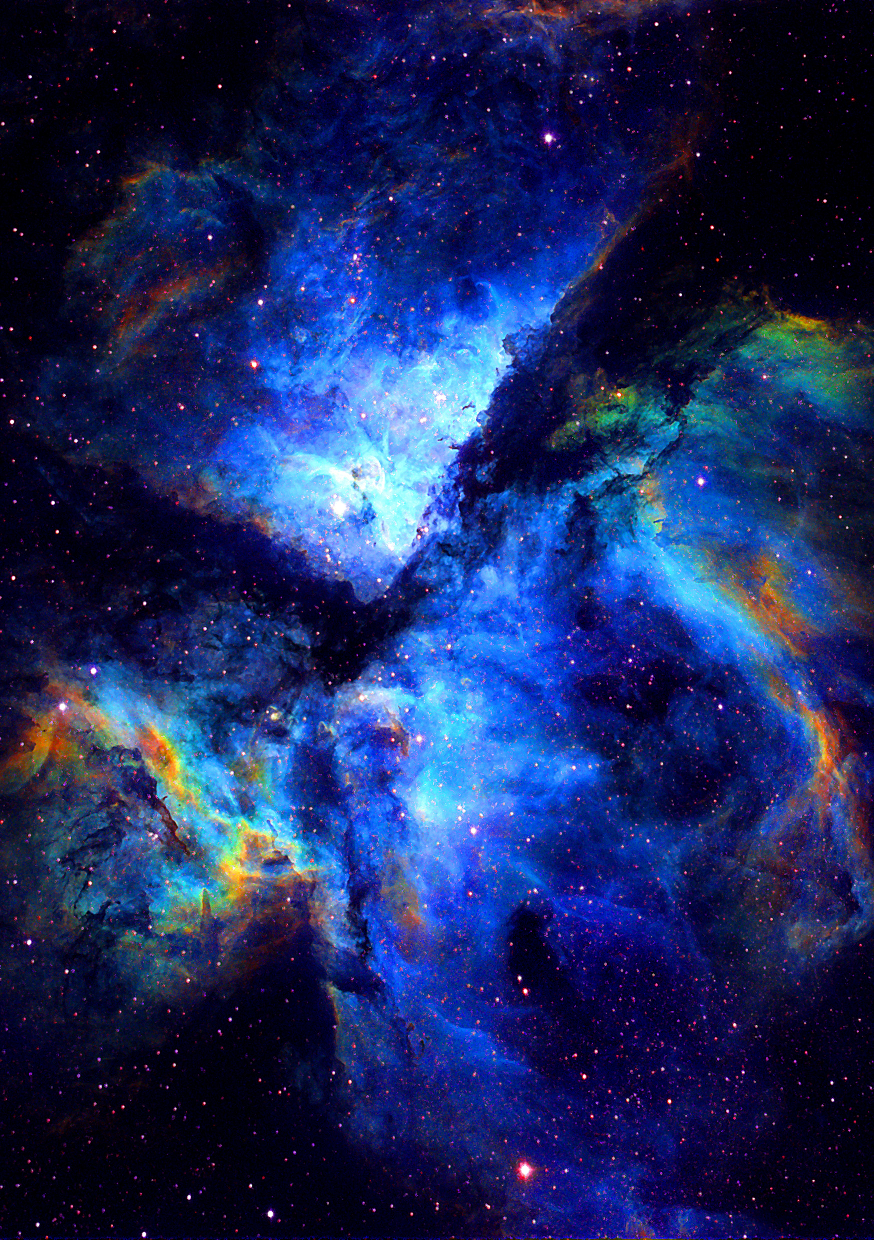
\includepdf[pages=-]{z-include-carinablue-a5.pdf}

Diesmal weniger gesund gestärkt, dafür aber sehr glücklich betrat Orakel die Zentrale. Er war mit sich und der Welt im Einklang, hatte zwei Jumbo-Pizzen verdrückt und grinste beim Blick auf die Außenbildschirme. Der Carinanebel erreichte darauf allmählich Dimensionen, die ihn auch ohne Vergrößerung gut erkennbar machten. Optisch hatte der Nebel einen hellen Rotton mit hauptsächlich 656,28 Nanometern Wellenlänge, der sogenannten »Wasserstoff-Alpha-Linie«. Orakel bevorzugte aus ästhetischen Gründen die blaue Darstellung der Sternenkarte und ließ sich den Nebel absichtlich in Falschfarben darstellen. Das hatte den angenehmen Nebeneffekt, dass auch unsichtbare Strahlung durch schöne bunte Farben dargestellt wurde. So sah der legendenumwobene Monsternebel viel einladender aus.

Mit einem Griff in die Erdnussdose auf seinem Kontrollpult begann der Navigator eine Situationsanalyse. Nüggät hätte längst aus dem Warpraum geholt werden können, doch die Abenteuergruppe um Knwrts verhielt sich passiv wie eine Fahne im Wind. Der Frust über den unerwünschten Besuch wich langsam der Überlegung, man könnte mit der Ezt Indüä Kmpnö kooperieren, müsste dies geradezu tun, um überhaupt eine realistische Fangchance zu erhalten. Änkäp, der blaurot gefärbte Äöüzz-Punk, war vielleicht noch am ehesten zu einem Zweckbündnis zu überreden. Büri hingegen war unberechenbar, hatte mehr als nur einen Schalk im Nacken sitzen und eine gehörige Meise. Knwrts hielt sie glücklicherweise regelmäßig davon ab, ihre Umgebung durch pure Tollpatschigkeit in Brand zu setzen. Am wenigsten wusste Orakel über Tllrk, den zweiten menschengroßen Käfer im Bunde. Dass dieser nun Doppelkopf spielen konnte und darin sogar yury überflügelte, schrieb Meister Orakel seinen großartigen Erklärungen zu. Womöglich spielte die Gruppe sogar genau jetzt das irdische Spiel, weiter von seinem Ursprungsort entfernt als jemals zuvor.

Schmerzhaft an die Abwesenheit seiner Freunde erinnert und mit einer düsteren Prophezeiung im Hinterkopf besann sich Orakel darauf, zu tun, was er für notwendig hielt. So war es ihm vor dem Gesetz und von Alexandra aufgetragen worden. Er hielt es allerdings für vollkommen legitim, sich bei dieser Entscheidung von einem bisher durch makellose Entscheidungen glänzenden Duo beraten zu lassen.

»Ich soll tun, was ich für notwendig halte«, eröffnete Orakel den Bordcomputern. »Könnt ihr damit etwas anfangen?«

Es war, als schwinge Verwunderung in der Computerstimme mit. \ialoudspeaker{»Ja.«}

»Und was heißt das jetzt?«, hakte Orakel nach.

\ialoudspeaker{»Das heißt, dass wir dir nicht bei der Beantwortung der Frage helfen. Helfen können, sagt der Siliziumteil. Helfen dürfen, sagt der Quantencomputer. Das Ergebnis bleibt gleich: Entscheide selbst.«}

Das war nach Orakels Ansicht zu viel Philosophie in zu kurzer Zeit und verlangte nach einer erneuten Stärkung. Knuspernd leerte er die Speisedose und starrte auf die Bildschirme. Noch war genug Wasserstoff vorhanden, um am Zielort zu agieren.

\begin{center}
∞∞∞
\end{center}

Tiefe Krater durchzogen die Landschaft eines namenlosen Zwergplaneten, dessen atmosphärelose Einsamkeit regelmäßig durch Steine aus dem All gestört wurde. Das ließ sich kaum vermeiden: Viele der einschlagenden Himmelskörper lagen mit zu geringer Eigengeschwindigkeit auf der Laufbahn des Namenlosen um seinen weit entfernten Vaterstern. Das gelbe Licht des ebenfalls namenlosen Sterns erhellte stets dieselbe Planetenseite~– »gebundene Rotation«, ein übliches Schicksal atmosphäreloser Planeten im Orbit massearmer Sterne.

Die roten Wolken des Carinanebels lagen derzeit auf der gegenüberliegenden Seite und füllten im dauerhaften Dunkel gut erkennbar den Sternenhimmel aus. Sterndichte und Zentrumsdistanz waren mit der Umgebung der Erde vergleichbar; ein blauer Riese stach in zwei Lichtjahren Entfernung leuchtend aus den Sternbildern hervor. Da keine Bevölkerung existierte, hatte niemand ihn oder seine Nachbarn am Himmelszelt getauft. Überhaupt hatte noch kein Lebewesen den Boden des Einsamen betreten. Irgendwann würde er durch die ständigen Einschläge zu Staub zerfallen, unspektakulär und unbedeutend in die Gemeinschaft eines Asteroidengürtels übergehen.

Durch vom Planeten nicht zu verantwortende Umstände wurde dieser zu einer Art Außenposten bei der Flucht einer zwielichtigen Gestalt aus dem Imperium von NGC 6193. Jahrmillionen nach Entstehen des Planetensystems kam endlich ein bisschen Leben in die Einöde: Drei fremde Flugkörper aus Metall und Kohlenstoffstrukturen schlugen parallel zur Bahnebene aus der Richtung des gelben Gestirns ein, zuerst golden, dann als weißer Torus, und mit gehörigem Zeit- und Raumabstand in blauer Keilform. Der goldene Lichtreflex hielt nahe an der physikalischen Velozitätsgrenze auf den einsamen Planeten zu, der Torus folgte in wenigen Kilometern Entfernung. Photonen tobten durch das All, doch was als zielgerichteter Laserstrahl den Verfolger verließ, traf nur diffus beim Verfolgten ein. Man hatte den optimalen Schussabstand verpasst und bemühte sich um eine Distanzkorrektur. Selbst die schnellen Prozessoren der automatischen Flugsteuerung hatten jedoch Schwierigkeiten, bei der relativistisch von innen empfundenen Hektik rechtzeitig eine Planetenkollision zu verhindern und die Däns Miräköl ins Visier zu nehmen.

Dögöbörz Nüggät war sich bewusst, dass kleinste Gesteinsbrocken wie Atombomben in seinen Schutzschirm einschlagen konnten. Dennoch ließ er sein Raumschiff mit halsbrecherischer Ungefesseltheit in eine Gegend rasen, die er für steinfrei hielt, auf die Nachfolger aber wie ein Minenfeld wirken musste.

»Nüggät spinnt«, stieß Orakel zwischen Flüchen hervor. Die Bordcomputer sahen das ähnlich und hatten längst Kurskorrekturen in Auftrag gegeben, die sich im Vergleich zur vorbeirauschenden Umgebung jedoch nur quälend langsam durch die Schiffsmechaniken propagierten. Für Orakel fand eine Achterbahnfahrt statt, auf die er gerne verzichtet hätte; Nüggät durchlebte mit stärkerer Begeisterung das gleiche Geschehen als Rennsport. Die beiden flogen in annähernder Lichtgeschwindigkeit am Polizeischiff P-2255 vorbei, das als Trojaner um den Lagrangepunkt L5 dem Planeten hinterherkreiste. Es nahm selbst dann keine Fahrt auf, als klar wurde, dass Nüggät mit seinem neu gewonnenen Überraschungsvorsprung in eine Warpblase flüchten würde. Nacheinander verschwanden die beiden Signale von der Umgebungserfassung.

\begin{center}
∞∞∞
\end{center}

Was auch immer den Gesuchten dazu bewogen hatte, seine Flucht auf alten Umwegen fortzusetzen: Die Däns Miräköl stattete dem Planetensystem einen zweiten Besuch ab. Aus der ehemaligen Fluchtrichtung kommend, schoss Nüggät mit seinem Gefährt durch die Nacht, überhaupt nicht zur Überraschung der noch immer parkenden Ezt Indüä Kmpnö. Bevor die Rückkehr am Lagrangepunkt optisch sichtbar wurde, kam Leben in das Polizeischiff.

Inzwischen sichtbar abgehängt platzte die 4-6692 aus ihrer Warpblase auf das Spielfeld, schubste einen Asteroiden mit einer Gravitationswelle so nachhaltig durch die Gegend, dass dieser seine Sternbindung verlor, und jagte fast hoffnungslos dem goldenen Triumphanten hinterher. Eher mit Neid als Bewunderung starrte Orakel die rechteckigen Markierungen auf seinen Monitoren an: Der unkontrollierbare Gewaltflug des Nuggets kreuzte genau dort die Flugbahn des Polizeischiffs, wo dieses bereits ausreichend Fahrt für einen Warpeintritt gesammelt haben würde. Das entzog sich jeder kausalen Erklärbarkeit, denn die Beschleunigung musste blind stattgefunden haben. Darüber hinaus fehlte eine Erklärung für die Rückkehr in ein System, das außer einem atmosphärelosen Zwergplaneten und dünnen Asteroidengürteln nichts zu bieten hatte.

Die noch mit Unterlichtgeschwindigkeit das All durchschießenden Abenteurer waren per Warpfunk erreichbar, würden sich durch ein Telefonat jedoch nicht aufhalten lassen. Orakel bemühte sich darum, wenigstens ein kurzes Statement zu erhalten: »Hey, habt ihr eine Zeitmaschine an Bord?«

\ialoudspeaker{»Mathematik.«} Das war eindeutig Änkäps Stimme, und mit diesem Wort verschwanden die zwei Rechtecke. Die 4-6692 beschleunigte länger als nötig, um den Warpantrieb zu schonen, und umgab sich nach einer halben Minute ebenfalls mit einer Warpblase.

Natürlich hatte sich das ursprüngliche Ziel des Fliehenden nie geändert. Der momentan in die falsche Richtung beschleunigende Goldklumpen vollzog daher einen erneuten Richtungswechsel, diesmal mit starker Umwegkurve im Warpraum. Er war sich seiner Sache so sicher, dass er ein Schneiden der Kurve durch das wendigere Verfolgerschiff in Kauf nahm. Die Verfolger verzichteten auf das technisch durchführbare Abfangmanöver und beharrten auf ihrer Beobachterrolle. Als dann die 4-6692 im Warpraum erschien, übernahmen deren Bordcomputer die Kursberechnungen und passten sich an das Geschehen an. Orakel erhielt die Initiative und nutzte diese, um so dicht an Dögöbörz Nüggät heranzufliegen, dass dessen Warpantrieb bei konstant 1.05c für seinen Piloten hörbar um einen Gnadenstoß bat. Anstatt noch näher heranzufliegen und das Zielobjekt auf Unterlichtgeschwindigkeit zu drücken, ließ Orakel den endgültigen Kurswechsel geschehen und wurde anschließend wieder langsam abgehängt.

\ialoudspeaker{»Warum hast du diese Chance verstreichen lassen?«}, fragten die Bordcomputer.

Orakel blickte nachdenklich dem Ortungsreflex hinterher. In dezimaler Schreibweise lief ein Tachometer voran: Dreifache Lichtgeschwindigkeit, vierfache Lichtgeschwindigkeit. »Ist das eine rhetorische Frage?«

\ialoudspeaker{»Das hängt von deiner Antwort ab.«}

»Ich habe mich nur an eure Anweisungen gehalten.«

\ialoudspeaker{»Dann«}, sprach da wohl der Quantencomputer, \ialoudspeaker{»darfst du die Frage als rhetorisch betrachten.«}

\iathought{Schönen Dank auch}, meckerte Orakel im Geist. Die Mission ging ihm langsam auf denselben. Andererseits schien es um deutlich mehr zu gehen als um rechtliche Geraderichtung nach moralisch grauen Taten. Die ganzen Vorhersagen klangen nach galaktischem Übel, und das ging sicherlich nicht von einem kleinen wichtigtuerischen Äöüzz-Barrensammler aus. Nüggät war nur ein Zahnrad in einem viel größeren Getriebe. Wie passend mechanische Begrifflichkeiten die Situation beschrieben, würden alle Beteiligten noch erfahren.

\cleardoubleevenpage

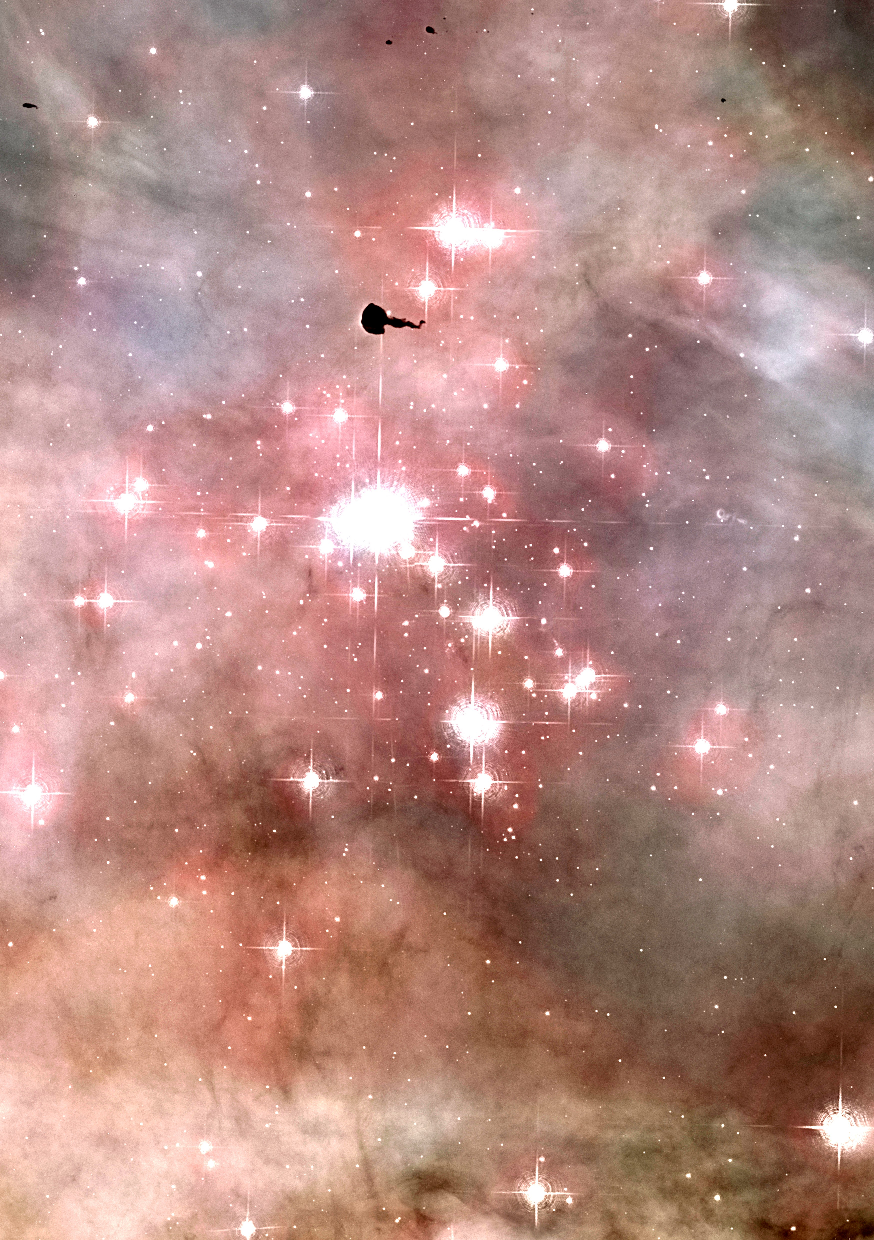
\includepdf[pages=-]{z-include-trumpler14-a5.pdf}

Das goldene Raumschiff steuerte einen Bereich des Carinanebels an, der auf der Erde als »Sternhaufen Trumpler 14« bekannt war. Das Innere solcher Sternhaufen war üblicherweise von starker Strahlung durchsetzt: Zweitausend Sterne teilten sich sechsunddreißig Kubiklichtjahre und beleuchteten die darin enthaltenen Planeten gemeinsam. Unter den Sternen von Trumpler 14 befand sich auch HD 93129, ein aus drei riesigen blauen O-Sternen bestehendes System, das drei Millionen Mal so hell wie Söl leuchtete und selbst über Örs mit bloßem Auge sichtbar war. Dauerhaftes Leben im Inneren dieses Infernos war nicht vorstellbar; eine Durchquerung mit Raumschiffen stellte bereits ein Abenteuer dar.

Orakel, dem aus irdischer Freizeitbeschäftigung diese Begebenheiten schon vor seinem ersten Weltraumflug bekannt gewesen waren, steuerte als Verfolger eines fast zu Fall gebrachten Flüchtenden auf einen Ort zu, der Kindheitserinnerungen an Astronomiebücher weckte.

\iathought{Geh jetzt und erledige, was du für notwendig hältst.}

Nein, ein Flug durch diese Weltraumgegend war definitiv nicht »notwendig«. Ließ dieser prophetische Spruch bei genauerer Betrachtung auch eine negative Auslegung zu? »Vermeide, was du nicht für notwendig hältst«, sinnierte Orakel vor sich hin und wurde stehenden Fußes von einer Lautsprecherstimme aus seinen Gedanken gerissen:

\ialoudspeaker{»Non sequitur. Es folgt nicht.«}

Orakel nahm erschrocken den rechten Daumennagel aus dem Mund und blickte symbolträchtig im leeren Kommandoraum umher. »Das Raumschiff folgt nicht? Ich folge nicht? Keine Verfolgungsjagd?«

\ialoudspeaker{»Wir möchten dich auf einen logischen Fehlschluss aufmerksam machen. Aus der zuvor von dir genannten Aufforderung kann nicht geschlussfolgert werden, dass zu vermeiden sei, was du nicht für notwendig hieltest. Das ist sachlich inkorrekt.«}

Welch ein Geschwurbel. »Könnt ihr das in weniger komplizierten Worten und ohne Latein erklären? Quintus habe ich vor Ewigkeiten hinter mir gelassen.«

\ialoudspeaker{»Selbstverständlich«}, antworteten die Bordcomputer gutmütig. \ialoudspeaker{»Stell dir vor, jemand sagt dir, du sollst morgens Wasser trinken.«}

»Das klingt nach einem gesunden Ratschlag«, befürwortete Orakel das Beispiel.

\ialoudspeaker{»Würdest du auf diesen Ratschlag hin nur noch morgens Wasser trinken?«}

Den Kopf schüttelnd, entgegnete Orakel: »Nein, natürlich nicht. Dadurch, dass Wasser am Morgen gesund ist, wird es zu anderen Tageszeiten ja nicht ungesund.«

Quod erat demonstrandum: \ialoudspeaker{»Wie kommst du dann darauf, du solltest Dinge vermeiden, die du nicht für notwendig hältst?«}

»Ah.« Orakel dachte angestrengt nach, was die Raumtemperatur seinem Gefühl nach um mehrere Örztemp erhöhte. »Wir werden Nüggät selbst dann verfolgen, wenn er direkt in die Hölle fliegt. Zumindest, solange unser Schutzschirm der Strahlung standhält. Da wir in dieser Hinsicht besser ausgerüstet sind als er, wird er absurde Manöver fliegen, um uns abzuschütteln. Ich möchte, dass ihr eure Wahrscheinlichkeitsbetrachtungen ein bisschen in Richtung ›Er weiß genau, was er sich erlauben kann‹ verschiebt. Der Typ hängt wie kein Mensch an seinem jahrhundertelangen Leben und wird jede wirkliche Gefahr geschickt vermeiden. Außerdem habe ich das Gefühl, er kennt sich in dieser Gegend erheblich besser aus als wir.«

Für den Navigator eines Äöüzz-Erkundungsschiffs mit all seinen Sternenkarten, Sensoren und direktem Draht zum Örz-Institut für interstellare Kommunikation war das ein erniedrigendes Eingeständnis. Auch der Quantencomputer tat sich intern schwer damit, Dögöbörz Nüggät auf seiner adrenalingesteuerten Panikmission als Fremdenführer zu akzeptieren. Der Siliziumcomputer gehorchte stumpf.


\chapter{Trumpler 14}

Die bunten Wolken, mit denen sich der Sternhaufen umgab, waren durch die Strahlung zum Leuchten angeregte Materie. Die statistisch für den Mittelteil des Durchflugs erwartbare Beinahe-Kollision mit einem Stern fand durch gezielte Provokation direkt am Eingangstor statt.

»Der spinnt doch«, sprach Orakel etwas aus, das der Quantencomputer ohne Höflichkeitsmechanismen sicherlich so unterschrieben hätte. Die Däns Miräköl war noch nicht ganz im Sternenhaufen angekommen, als sie bereits eine ruckartige Kursanpassung vornahm und unter großer Warpbelastung einen hellblau brennenden B-Stern anvisierte. Die Fluggeschwindigkeit sank innerhalb weniger Minuten auf ein halbes Lichtjahr pro Stunde ab, was nach galaktischen Maßstäben ein quälendes Schneckentempo darstellte. Lokal betrachtet schoss die 4-6692 auf einen Flammenball zu, und Bremsen war während der Verfolgungsjagd keine Option. Dass die Geschwindigkeit dennoch sank, war dem Masseeinfluss des Sterns zu verdanken. Ein Verglühen ließ sich so jedoch nicht verhindern.

Nüggät ließ den Warpantrieb seines Raumschiffs annähernd tangential auf die zwanzigtausend Kelvin heiße Chromosphäre zusteuern. Die Außenansicht war ohne elektronische Nachbearbeitung nicht mehr zur Orientierung zu gebrauchen, weil das Lichtermeer von Trumpler 14 bereits Photonenströme auf die Sensoren einprasseln ließ, die in menschlichen Augen zur sofortigen Erblindung geführt hätten. Niemand, absolut niemand, außer Dögöbörz Nüggät, kam auf den Gedanken, sich auf diesem stellaren Chaosball einen Tanzpartner zu suchen. Und niemand außer Orakel griff in einer solchen Situation nach Schokoladenkeksen.

»Wenn er nicht abdreht, verbrennt er einfach.« Orakel riss die Packung auf und entnahm ihr den ersten Keks. »Wir müssen davon ausgehen, dass er den Kurs kurzfristig so abändert, dass er über fünf Sterndurchmesser Distanz behält.«

Die Bordcomputer markierten in einer Vergrößerungsansicht die besagte Flugbahn. Sie unterschied sich im entscheidenden Bereich erheblich von der aktuellen Projektion.

»Bitte färbt die Lichtgeschwindigkeitsgrenze unserer Warpantriebe in unterschiedlichen Rottönen ein.«

Daraufhin umgaben zwei konzentrische Sphären den Stern, beide durchschnitten von der aktuellen Fluglinie. Das kleine goldene Klümpchen war empfindlicher gegenüber gravitativen Einflüssen als die verhältnismäßig große 4-6692. In Gedanken an kleine Wüstenmäuse und große Eisbären fragte Orakel sich allerdings, weshalb es die Hitze des blauen Riesen nicht besser reflektieren und ableiten konnte als das Erkundungsschiff. Er teilte den Bordcomputern diese Überlegungen mit und wurde sogleich belehrt:

\ialoudspeaker{»Diese Faustformel gilt nur im Biologieunterricht auf Planeten. In der unmittelbaren Nähe von Sternen bedeutet eine größere Oberfläche vorrangig eine stärkere Angriffsfläche für Strahlenabsorption. Größeres Volumen dient hingegen, wenn du es so nennen möchtest, nicht als Wärme-, sondern als Kältespeicher. Zudem ist unser Raumschiff weiß lackiert. Dass Nüggäts Raumschiff im sichtbaren Licht eine andere Farbe hat als unseres, liegt daran, dass Gold Strahlung unterhalb von fünfhundert Nanometern Wellenlänge zu über sechzig Prozent absorbiert. Das mag in gelbem Sonnenlicht nicht besonders auffallen, wird neben einem B-Stern aber extrem schmerzhaft.«}

Da Dögöbörz Nüggät sich über die Verwundbarkeit seiner Eitelkeitslackierung bewusst war, verzichtete er auf das Experiment. Mit sanften Stößen gegen die Tangente drückte er die Däns Miräköl von der chromosphärischen Flugrichtung weg ins All. Ungefähr dreizehn Sternradien sollten es sein. Orakel, bei dem die Kursänderungen zeitlich verzögert, aber am selben Ort erfolgten, biss bei jedem Stoß in das Gebäck. Es dauerte viele Minuten, bis Schokolade und Sensordaten ein Lächeln auf die Bildschirme zurückfallen ließen. Ein wenig Häme, nur ganz wenig, das Gefühl sanfter Schadenfreude mischte sich mit der Erleichterung: Nüggät hatte nie eine andere Wahl gehabt und musste sich eine gewisse Unterlegenheit gegenüber dem irdischen Emporkömmling eingestehen. Diese rührte auch nicht ausschließlich von der Technik her: Mit Orakel hatte ein Optimist den Sternennebel betreten, der sich unvoreingenommen durch den Legendensumpf schlug.

Der Temperaturanstieg war in der Zentralkugel nicht spürbar, weil die 4-6692 dem Stern ihre kleinstmögliche Stirnfläche zuwandte und die Klimaanlage die Hitze im unbewohnten Außenring verteilte. Der Edelmetallhändler jedoch geriet gehörig ins Schwitzen und wünschte sich, einen größeren Abstand gewählt zu haben. Viel zu nah zog die hellblaue Scheibe auf der Außenansicht vorbei, umfasste kurzzeitig knapp neun Grad des Bildschirmkreises und verschwand in der Ferne. Bis jedoch die thermischen Auswirkungen des Systembesuchs abgeklungen waren, vergingen mehrere Stunden …

\begin{center}
∞∞∞
\end{center}

…, wenn man den Prozess nicht mit Wasser beschleunigte. Inmitten eines lebensfeindlichen Strahlenmeers, zweihundert astronomische Einheiten von seinem blauweiß leuchtenden Doppelstern entfernt, wartete ein ganzer Planet überzogen mit der kostbaren Abkühlung. Die Pole waren gefroren, die Äquatorregion von milden Dampfwolken bedeckt. Eine dichte Sauerstoffatmosphäre rundete das Bild ab.

Idyllisch sah die Wasserwelt aus der Ferne aus, einladend blau. Durch die Sternenfarbe kam das Dihydrogenmonoxid besonders schön zur Geltung. Still und starr lag die See. Kein Fisch, keine Wasserpflanze gedieh unter dem beißenden Ultraviolett. So war das blauweiße Nass ganz ohne Chlorbeigabe steril und dennoch nicht zum Schwimmen geeignet.

Dögöbörz Nüggät liefen unter seinem grünen Fell die Schweißtropfen von der Stirn. Eine kühle Dusche im Schutz des Raumschiffs, aber mit dem frischen Wasser von draußen, war lange überfällig. Das goldene Nugget fädelte sich in eine Umlaufbahn ein, ging im Bereich von 368 Örztemp über dem Äquator nieder, ließ einen Kometenschweif über dem Horizont aufblitzen und tauchte mit vierhundert Metern pro Sekunde ab. Die Überschalldruckwelle ließ das Wasser verdampfen, das Raumschiff in den Dampf einschlagen und die Fahrt durch den entstandenen Unterdruck von hinten stark abbremsen. Die Däns Miräköl war unterwasserfähig und bewegte sich mit Turbinen weiter voran, deutlich langsamer als in der Atmosphäre, mit fünf Metern pro Sekunde.

Orakel beobachtete den Tauchvorgang aus der Ferne. Er hatte mit der 4-6692 einen gemütlichen Orbit um die Wasserwelt gewählt und besaß genug Wasser an Bord, um sich im Bordpool ein Hörbuch zu gönnen. Auf den Bildschirmen des Wellnessbereichs bewegte sich eine Unterwassermarkierung unter den langsam verebbenden Einschlagswellen. Es bestand die Möglichkeit, einen Normalfunkspruch zu senden, doch die beiden Rivalen hatten sich bereits alles gesagt, was es zu sagen gab. Auch von der Planetenoberfläche kam kein Funkspruch zu ihm herauf.

Mit Kohlensäure versetzt wäre selbst hundertfach wiederverwertetes Abwasser schmackhaft gewesen, doch dieses Glas enthielt entsalzenes Frischwasser vom Planeten Wildfalle. Die Vorräte waren riesig. »Kann mir jemand kurz berichten, was aus dem Polizeischiff geworden ist?«

\ialoudspeaker{»Von der Ezt Indüä Kmpnö fehlt jede Spur. Es bestand zuletzt eindeutig die Möglichkeit, die Verfolgung zu eurem Vorteil zu beenden. Keiner hat sie genutzt. Auch jetzt könntest du eigentlich deine Position für einen Sturzflug und einen Nahkampfangriff nutzen.«}

»Das würde sich nicht richtig anfühlen.« Orakel bog sich knackend nach hinten. Irgendwo wurde ein Nerv getroffen und ein heißer Puls zog sich durch den gesamten Körper. »Das ist ein bisschen so, als würde man auf einen Verwundeten schießen.«

\ialoudspeaker{»Nüggät ist ein Äöüzz. Er weiß genau, dass er einen fairen Prozess vor den Gerichten seines Heimatplaneten erwarten kann. Wenn er sich dennoch aktiv der Verhaftung entzieht, gibt es keinerlei moralischen oder rechtlichen Bedenken dagegen, sein Fluchtgefährt flugunfähig zu schießen und ihn nach Örz zu überführen.«}

»Ist das nicht genau das, was er auf El Dörädö getan hat?«

\ialoudspeaker{»Möglich. Man wird das gerichtlich beurteilen müssen, ganz besonders mit Blick auf deinen Ex-Bekannten Floating Island.«}

Orakel verschluckte sich fast. »Ihr meint, Island ist tot? Nüggät ist kein Mörder.« Nein, so unmoralisch war der Edelmann sicherlich nicht.

Die Bordcomputer enthielten sich einer themenbezogenen Antwort und wechselten übergangslos zum Tagesgeschehen. \ialoudspeaker{»Der Wasserstoffvorrat ist nicht mehr in einem Zustand, der sich zum Start einer Langzeitexpedition eignen würde. Wir haben auf Wildfalle zwar das Trinkwasser ausgetauscht und genug Konserven für jahrzehntelanges Überleben in einem Atombunker an Bord, aber dein kleines Wettrennen zwischen den Sternen war energetisch äußerst teuer.«}

»Nüggät wird es dann wohl ähnlich gehen. Aber wenn wir eine Tankpause einlegen, fliegt er uns davon.«

\ialoudspeaker{»Nüggät denkt vor allem wirtschaftlich. Und nur zur Erinnerung für dich, Örsmensch: Er ist in der extremsten Form von Kapitalismus aufgewachsen, die in der Galaxis bekannt ist. Du könntest versuchen, einen Vertrag auszuhandeln.«}

Nun musste Orakel lachen. »Das sieht euch ähnlich. Das Gleiche gilt für euch. Ich werde jedenfalls einen Teufel tun, mit dem Trickser da unten zu verhandeln. Im Zweifelsfall haben wir den längeren Atem. Das ist doch so, oder?«

Unumwunden erhielt er von den Computern die Bestätigung, dass die 4-6692 trotz höherer Masse und höherem absolutem Treibstoffverbrauch generell effizienter als die Däns Miräköl arbeitete. Das Erkundungsraumschiff war für genau solche Situationen gebaut worden, das kleine Individualschiff war ein Prestigeobjekt und diente üblicherweise nur zum Personentransport innerhalb der Äöüzz-Wirtschaftsvereinigung. Diese war von Tankstellen durchzogen, die mitten im All schwebten oder zumindest auf Planeten ein schnelles Auftanken mit reinem Wasserstoff anboten.

Der schon wieder hungrige Navigator schloss daraus, dass Nüggät früher oder später um einen gnadevollen Tankstopp betteln musste. Auf den Monitoren waren die Wellen inzwischen verschwunden und die möglichen Positionen des U-Boots als grüner Kreis eingefärbt: Da wurde jemand nicht gerne beobachtet und hatte sich in ortungsresistente Tiefen zurückgezogen. Orakel sah das mit Gelassenheit, denn er konnte jederzeit seinen Orbit verändern, um den Überblick auszudehnen oder die Umlaufzeit zu verringern. Irgendwann musste Nüggät auftauchen. Selbst falls das auf der anderen Seite des Planeten geschah, blieb genug Zeit für eine Verfolgung durch das Weltall. Der Planet ließ sich dabei nicht dauerhaft als Ortungsschutz zwischen die Schiffe schieben, denn der Fliehende besaß seinerseits nicht die zum Ausweichen notwendigen Informationen. Die Bordcomputer der 4-6692 variierten den Kurs, um Vorausberechnungen in Abwesenheit unmöglich zu machen. Wenn Nüggät sehen wollte, wo sich der Verfolger befand, musste er sich seinerseits zu erkennen geben. Floh er blind, durchkreuzte er Orakels Sichtfeld.

Nach einem ausgiebigen Abendessen verabschiedete Orakel sich in Richtung seiner Kabine. Bei aller Gelassenheit fiel es ihm schwer, den nun wirklich überfälligen Schlaf zu finden, um Kraft für weitere Verfolgungsflüge zu sammeln. Die Bordcomputer halfen subtil nach, indem sie allmählich die Helligkeit und den Blauanteil der Außenansicht an den Kabinenwänden verringerten.

\begin{center}
∞∞∞
\end{center}

Am nächsten Morgen begab sich Orakel in die Kantine, brachte mit einer Mischung aus Zucker und Vollkorn seinen Kreislauf einigermaßen nachhaltig in Schwung, betrat mit wehmütigem Blick an Frees Kabinentür vorbei den Nordgang und verharrte im gläsernen Zwischenraum, um den Flug über die Planetenoberfläche zu genießen. Draußen ging zum fünfzigsten Mal an diesem Tag die Sonne auf. Das blauweiß blendende Licht wurde durch Elektronik im Glas und den Schutzschirm gedämpft; besonders die kurzwellige Strahlung außerhalb des sichtbaren Bereichs wurde absorbiert. Dennoch hätte Orakel ein Sonnenbad nehmen können, wenn er gewollt hätte.

Er wollte nun aber vor allem eines: Nüggät beim Auftauchen erwischen und sich ihm erneut an die Fersen heften. In der Zentrale angekommen, forderte er einen kurzen Lagebericht an.

\ialoudspeaker{»Das mutmaßliche Hauptziel des Eintauchens, die Abkühlung nach dem Sternenflug, ist längst erreicht. Auch wir haben inzwischen ganz ohne Wasserberührung die Temperatur abgebaut, die sich im Außenring angestaut hatte. Zum Trinkwasseraustausch bestand ebenfalls mehr als genug Gelegenheit. Das derzeitige Verharren unter der Wasseroberfläche ist nur durch Schlaf oder Zermürbungsversuche zu erklären.«}

»Letzteres wäre ziemlich dämlich«, beurteilte Orakel die Möglichkeiten. »Ich habe hier oben einen Wellnessbereich, ein Sportzentrum, ein Tonstudio und abwechslungsreiches warmes Essen. Wenn mir danach ist, kann ich in Hörbüchern schwelgen, deren Gesamtdauer die Lebenserwartung eines Äöüzz übersteigt. Und ich kann an meinem Tagebuch weiterschreiben, bis der Arzt kommt.«

\ialoudspeaker{»Wir wagen zu vermuten, dass du die Geduld und die Leidensbereitschaft deines Jagdobjekts deutlich unterschätzt. Auch dein eigenes Leben ist begrenzt; deine Freunde machen sich irgendwann Sorgen um dich. Wir können uns auch nicht wirklich vorstellen, dass du mehrere Jahre lang hier verharren möchtest, wo es doch immer die winzige Möglichkeit geben wird, dass Nüggät längst unbemerkt geflohen ist.«}

Die Stirn runzelnd, entgegnete er: »Ich dachte, Nüggät kann objektiv nicht unbemerkt fliehen.«

\ialoudspeaker{»Es ist unwahrscheinlicher als ein Lottogewinn, aber es wird dich auf Dauer zermürben, dass du mit der Wahrscheinlichkeit eines Lottogewinns bis an dein Lebensende hier auf jemanden warten musst, der längst geflohen ist.«}

Und die verdammten Bordcomputer hatten wie immer recht. »Der grüne Kreis ist derzeit noch überschaubar. Können wir das Wasser irgendwie durchkämmen?«

Es bestand die Möglichkeit, zivile Sonardrohnen abzusetzen. Die entsprechende Programmierung und Bestückung an den Mehrzweckrobotern war bereits vorgenommen worden und Orakel entschied sich zu ihrem Einsatz. Kurz darauf verließ ein Schwarm insektenähnlicher weißer Flugobjekte die Bodenluke des Schiffs und verteilte sich über den kreisförmigen Bereich der Wasseroberfläche, unter dem Nüggät sich derzeit befinden konnte. Alle Mitglieder des Schwarms tauchten zeitgleich unter die Wasseroberfläche und sendeten Schallsignale zur Ortung aus.

»Hättet ihr das auch ohne mich getan, wenn der Kreis zu groß geworden wäre?«

\ialoudspeaker{»Ja, aber es bestand keine Eile. Der Kreis wäre auch in einigen Tagen noch durchkämmbar gewesen. Die Möglichkeit, direkt hinterherzutauchen und Waffen einzusetzen, hattest du ja absichtlich verstreichen lassen.«}

»Gut.«

\begin{center}
∞∞∞
\end{center}

Der Ozean war tief, doch die Druckbeständigkeit eines Raumschiffs hatte ihre Grenzen. In fünfzig Metern Tiefe bestand ohne energiefressende Schirmunterstützung ein gutes Mittelmaß zwischen Unsichtbarkeit und Wasserdruck. Für die Echolot-Roboter der 4-6692 stellte diese Tiefe jedoch keine Herausforderung dar. Nur wenige Minuten nach Beginn der Suchaktion reflektierten tieffrequente Schallwellen an der Außenhülle der Däns Miräköl.

»Das ging schneller als erwartet«, freute sich Orakel.

»Das ging schneller als befürchtet«, ärgerte sich Nüggät. »Wir warten noch, bis der Donut eintaucht, dann machen wir uns aus dem Staub.«

Als die 4-6692 ihre Ortungsgeräte wieder eingesammelt hatte und dazu ansetzte, über der Däns Miräköl ins Wasser abzutauchen, um diese notfalls durch Herunterdrücken in die Tiefsee zur Aufgabe zu zwingen, schlug Nüggät einen Haken und schoss empor. Orakel sah noch erschrocken auf die optische Erfassung, als die Bordcomputer das Manöver bereits verarbeitet und einen Notstart veranlasst hatten. Nun machte sich die größere Masse des Erkundungsschiffs bemerkbar; schwerfällig löste sich der weiße Torus aus dem Wasser, hinterließ kreisförmige Wellen und schaltete frühzeitig den Raketenantrieb hinzu. Der gelbe Komet durchstieß die Stratopause und stellte seinen Verfolger vor physikalische Herausforderungen.

Leicht angesäuert drückte Orakel seine geballten Hände hinten auf das Bildschirmpult. Seine Arme schlossen ein immer kleiner werdendes Bild der Däns Miräköl ein, bis der Informationsgehalt unter einen Schwellwert fiel. Die Darstellung wurde durch eine gerenderte Außenansicht der Planetenkugel ersetzt, aus der ein Raumschiff ins All schoss. Entscheidend war nun vor allem, wie früh der Warpantrieb gezündet wurde: Wie stark legte Nüggät es überhaupt darauf an, nicht verfolgbar zu sein? Auf Kosten der Bauteile bot sich hier möglicherweise ein schmerzvoller Fluchtsprung an.

Tausende Lichtjahre von der Wirtschaftsvereinigung entfernt vermied der Solo-Fluchtpilot das Herbeiführen eines Wartungsfalls. Der Vorrat an Ersatzkondensatoren war vor der Sabotageaktion geschrumpft und seitdem nicht nachgefüllt worden. Ein verfolgtes Raumschiff war besser als ein kaputtes Raumschiff.

Erst, als die Wasserwelt drei Lichtminuten entfernt und kaum noch mit bloßem Auge zu erkennen war, zündete Nüggät den Warpantrieb. Deutlich näher am Planeten hatte die 4-6692 inzwischen stark genug beschleunigt, um einen Verfolgungsflug zumindest unmittelbar reparaturlos zu überstehen. Im Weltall zeigten sich erneut die Vorzüge des hochwertigen Äürörä-Überlichtmoduls.


\chapter{Carinas dunkles Geheimnis}

Auf Dögöbörz Nüggäts Schiff studierte ein ausgeschlafener, weitestgehend medizinisch reparierter Äöüzz mit noch nicht vollständig getrocknetem Fell einen Bildschirm gegenüber der Nasszellentür.

\iathought{Sobald das Tor entriegelt ist, gibt es kein Zurück mehr}, zitierte der Pilot im Gedächtnis. Alles, was im Brief stand, war auf geheimnisvolle Weise eingetreten. Und obwohl ihm ein Regenbogen als der Beginn einer neuen Ära vorausgesagt worden war, scheute er davor zurück, die Konsequenzen aus den Ratschlägen zu ziehen. Es war keine leichte Entscheidung, die ihm bevorstand.

\noindent \parbox{\textwidth}{ \vspace{3ex} \hrule \vspace{3ex}

\iaquote{Du siehst, wohin du siehst, nur Eitelkeit auf Erden.\\
Was dieser heute baut, reißt jener morgen ein:\\
Wo jetzt noch Städte stehn, wird eine Wiese sein,\\
Auf der ein Schäferskind wird spielen mit den Herden.}

\iaquote{Was jetzt noch prächtig blüht, soll bald zertreten werden.\\
Was jetzt so pocht und trotzt, ist morgen Asch’ und Bein,\\
Nichts ist, das ewig sei, kein Erz, kein Marmorstein.\\
Jetzt lacht das Glück uns an, bald donnern die Beschwerden.}

\iaquote{Der hohen Taten Ruhm muss wie ein Traum vergehn.\\
Soll denn das Spiel der Zeit, der Einzelne bestehn?\\
Ach! Was ist alles dies, was wir für köstlich achten,}

\iaquote{Als schlechte Nichtigkeit, als Schatten, Staub und Wind;\\
Als eine Wiesenblum’, die man nicht wieder find’t.\\
Noch will, was ewig ist, kein Einziger betrachten.}

\vspace{3ex} \hrule \vspace{3ex} }

Nüggät seufzte. »Kann nichts dich, Fliehende, verweilen, oh meines Lebens goldene Zeit? Vergebens, deine Wellen eilen, hinab ins Meer der Ewigkeit.«

Es gab nur eine mögliche Deutung: Die Reise musste durch den Schlüssellochnebel führen; kein anderes Objekt im Carinanebel kam als Ziel dieser Metapher infrage. Dem Hinweis mangelte es an Subtilität und Kreativität, und der Verfasser des Briefes hatte kein Interesse daran gehabt, den Leser in die Irre zu führen. Das »Tor« war der gesamte Nebel, und er umschloss irgendetwas Grauenvolles, einen Quell des Verderbens, eine Zeitbombe. Unfreiwillig zu einer Art Minenräumkommando geworden, durchflog Nüggät ohne weitere Provokationen den Sternhaufen, stellte das Abhängen seines irdischen Gegenspielers vorerst an das Ende seiner Prioritätenliste und steuerte auf ein dunkles Gebilde zu. Dessen Bezeichnung als das »Schlüsselloch des Carinanebels« stammte aus dem Jahr 1873, in welchem die irdische Autorin Emma M. Converse die »Herschel'sche Lemniskate« in Appletons’ zehntem Journal als »schlüssellochförmige Höhle« beschrieben hatte. Die »Höhle« durchmaß sieben Lichtjahre, sah tatsächlich wie ein schwarzes Schlüsselloch aus und wirkte auch ganz ohne Legenden eher bedrohlich als gastfreundlich.

Ungefähr zwanzig Lichtjahre vom Dunkel entfernt befand sich ein brauner Zwerg, ein wie Jupiter aussehender Gasplanet, der durch seine zwanzig Mal größere Masse bereits rötlich leuchtete. Im Gegensatz zu Sternen fand in braunen Zwergen keine normale Wasserstofffusion statt: Dreizehn Jupitermassen reichten zur Deuteriumfusion aus, doch erst achtzig Jupitermassen verwandelten Himmelskörper in echte Sterne, in denen Protium zu Helium wurde. Der braune Zwerg galt daher nicht als »Stern« und leuchtete trotzdem. Tiefrot, größtenteils unterhalb des sichtbaren Frequenzbereichs, erwärmte er …

\bigskip

… nichts.

\begin{center}
∞∞∞
\end{center}

»Der edle Äöüzz wird vermutlich gleich hier eintreffen und sich gehörig wundern.« Knwrts klapperte mit seinen bunten Greifzangen. Das Chitintrihalogenid in seiner Nahrung hatte den gesamten Käferkörper in ein irisierendes Kunstwerk verwandelt, das dem Piloten der Gruppe würdig war. Änkäp, der individualistisch autoritätsfeindliche Äöüzz, erinnerte ihn gelegentlich an seine Ranggleichheit mit der restlichen Besatzung. Eines hatten alle vier Abenteurer gemeinsam: Ein stetes Streben nach möglichst wertvollem Besitz. Klassische Definitionen von Eigentum waren ihnen suspekt: Solange nicht eine höhere Macht eingriff und die Besitzverhältnisse umstieß, besaß jeder nur das, was er selbst gegen andere verteidigen konnte. Das galt für das waffenstarrende Polizeiraumschiff ebenso wie für das Gold im Frachtraum: Kontostände waren der Ezt Indüä Kmpnö egal, auf Gutscheine jedes Ausstellers wurde gepfiffen und jeder war sich selbst der Nächste. Mit den Strukturen der Äöüzz-Wirtschaftsvereinigung arrangierte sich das Quartett recht gut, da der dortige Kapitalismus gerade genug mit den anarchistischen Werten gemeinsam hatte, um ihn auszunutzen, statt ihn zu bekämpfen. Kopfgelder wurden dankend angenommen, sofort in Metall verwandelt und für weitere Abenteurer genutzt: Raumschiffe, Goldbarren, Waffen und eine gehörige Portion Übermut ballerten sich rücksichtslos durch das All. Neider gab es seit Ewigkeiten, Feinde nur für kurze Zeit.

Die P-2255 hatte die Däns Miräköl nicht nur tagelang unbemerkt verfolgt, sondern diese nun auch noch im Warpraum überholt. Der merkwürdige Vielfraß von Örs hielt sich für einen großen Verfolger, doch er besaß weder die Waffen noch den Mumm, um Nüggät zu stoppen. Hier spielten Profis ein gefährliches Glücksspiel außerhalb Orakels Liga.

Als das goldene Raumschiff eintraf, wurde es von einem Gravitationsstoß in Flugrichtung erschüttert. Der Schutzschirm leuchte auf, als eine Hochgeschwindigkeitskollision stattfand. Peripher, aber bei den vorherrschenden Geschwindigkeiten beinahe fatal: Ein streifendes Ramm-Manöver an der Oberseite. Dazu gab es den folgenden Funkspruch: \ialoudspeaker{»Schluss mit den Spielchen. Mit diesem System stimmt irgendetwas nicht, und wir verlangen eine Erklärung.«}

»Macht ihr Witze?«, schrie Nüggät mit aufgerissenen Augen in seine Mikrofone. Die Bordelektronik war gut damit beschäftigt, den Kollisionsschaden zu beheben. Dass die Außenhülle noch stand, war ein Wunder. »Das Einzige, was mit diesem System nicht stimmt, ist eure Anwesenheit!«

\ialoudspeaker{»Die möchten wir ja gar nicht bestreiten«}, funkte Büri. \ialoudspeaker{»Aber das ist jetzt das zweite Mal, dass die Kartensignatur nicht mit dem Systeminhalt übereinstimmt. Du scheinst dich hier besser auszukennen als jeder andere Äöüzz, also raus mit der Sprache: Was wird hier gespielt?«}

Nüggät nahm die Nachricht ernst. Während er kollisionslos das Polizeischiff überholte, wertete er die Außenüberwachungsdaten aus. Ein Y-Zwerg mit einer Masse von ungefähr 8,46×10²⁸ ISG leuchtete im nahen Infrarot vor sich hin. Andere Objekte waren nicht zu sehen. »Wo sind die Monde?«

\ialoudspeaker{»Es würde uns ungemein beruhigen, wenn du uns das erklären könntest. Wir verstehen da auch relativ wenig Spaß.«} Die Ezt Indüä Kmpnö hielt nicht viel von wörtlichen Warnungen; Tllrks Laser kamen bereits zum Einsatz. Für die vorlädierten Schutzschilde wurde es brenzlig, doch Nüggät konnte bei bestem Willen nicht die geforderte Antwort liefern.

»Ich sehe ja ein, dass ihr gerade am längeren Hebel sitzt. Mir ist auch bewusst, dass ihr mich eher verglühen lassen würdet, als auf die Antwort zu verzichten, denn hier ist wirklich irgendetwas Merkwürdiges geschehen. Wir haben das bei unserem ersten Stopp vor dem Nebel vermutlich gemeinsam bemerkt, und nun sind die Monde in diesem System ebenfalls verschwunden. Spurlos: Keine Gaswolke, kein Trümmerhaufen. Gut, vielleicht sind alle Trümmer restlos ins Deuterium gestürzt, aber das haltet ihr wohl ebenfalls für eine schlechte Ausrede.«

Da die Laser sich unbeirrbar voran fraßen und das Kraftwerk erheblich belasteten, blieb Nüggät nur noch die Flucht. Man würde ihm ohnehin nicht glauben, dass er mit dem Verschwinden der Himmelskörper nichts zu tun hatte. Die Geschwindigkeit war gut, aber die Masse des Polizeischiffs verhinderte derzeit einen Sprung. Zum zweiten Mal trat Nüggät das Notfallpedal durch; diesmal lag die Überraschung auf Büris Seite. Woher kam diese Beschleunigungskraft?

Das Goldschiff war schneller verschwunden, als die P-2255 ihre Kraftwerksleistung anpassen konnte. Ähnliches war zuvor Orakel widerfahren, der sich bereits in überlegener Position gesehen hatte. Das Überraschungsmanöver war eine wertvolle Lebensversicherung, aber es lag in seiner Natur, dass es jedem Gegner gegenüber nur einmal genutzt werden konnte. Noch einmal würde sich Büri nicht überrumpeln lassen.

Orakel kam gerade rechtzeitig an, um den Fluchtsprung zu sehen und sofort wieder in den Warpraum überzugehen. Die Besatzung der P-2255, die sich gerade per Funk an ihn wenden wollte, redete gegen eine Wand und fühlte sich endgültig an der Nase herumgeführt. Ungehalten nahm sie als Schlusslicht an der Kolonne teil.

\cleardoubleevenpage

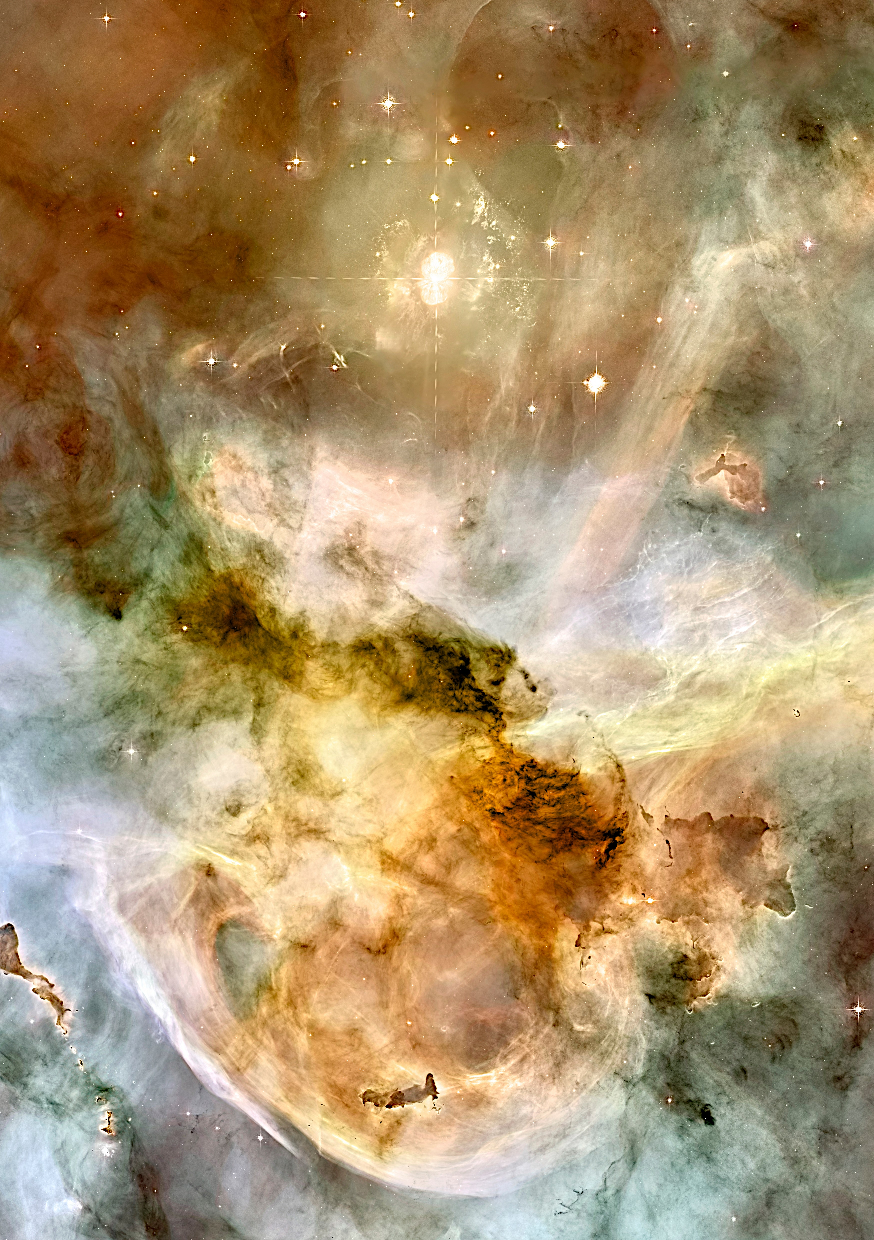
\includepdf[pages=-]{z-include-etacarinaekeyhole-a5.pdf}

Dunkelheit umschloss den Eindringling. Sie umspülte ihn mit Sternenstaub, grauschwarzer Masse, die alle umgebenden Sterne verdunkelte und das Weltall mitten im Carinanebel wieder aussehen ließ wie die Bereiche fernab davon. Trumpler 14 war schwach zu erkennen, Eta Carinae wirkte wie ein Vollmond in düsteren, bewölkten Erdnächten. Die Umgebung lud zum Gruseln ein, war ansonsten abstoßend und als Tourismusziel bereits durch ihre Unübersichtlichkeit ungeeignet. Kein Fremdenführer wäre dazu in der Lage gewesen, naiven Sonntagsfliegern in diesem Dickicht eine sichere Navigation zu ermöglichen. Wer sich in diesen Nebel begab, tat dies auf eigenes Risiko: Sternlose Planeten und Asteroiden durchzogen den Staub, waren mangels Reflexion nahezu unsichtbar bis zur Kollision und wirkten wie ein Minenfeld.

Den bekannten Dichtedaten widersprechend fand auch eine starke Beeinflussung des Warpantriebs statt. Der Schlüssellochnebel war längst nicht mehr das seidene Gebilde, das auf Örs zu sehen war; in den letzten Jahren waren Veränderungen eingetreten, die optisch weder Örs noch Örz erreicht hatten. Da half kein Teleskop: Was hier geschehen war, würde man auf der Erde erst in tausenden Jahren bemerken.

Dögöbörz Nüggät bemühte sich, durch Kursänderungen ein zweites Abfangmanöver zu verhindern, ohne dabei sein Raumschiff in einen der zahlreichen Felsbrocken rasen zu lassen, die den Nebel erschreckend hochfrequent durchzogen. Das war niemals natürlich entstanden und erklärte möglicherweise das Fehlen ganzer Planetenmassen außerhalb des Nebels. Jemand hatte die Planeten und Monde gestohlen und im Schlüsselloch zerbröselt. Keine Macht der Galaxis, nicht einmal die Äöüzz, verfügte über die technischen Mittel für eine derart groß strukturierte Umformungsaktion. Die Legende vom »Monster des Carinanebels« gewann an Substanz.

Büri sah eine Kursänderung um ungefähr 90 Grad nach links und bildete mit ihrem Kurs die zugehörige Hypotenuse. Bevor sich das Dreieck schloss, war der Verfolgte jedoch bereits schräg nach oben abgebogen. Alles geschah im Schneckentempo, weil die Warpantriebe sich an der Umgebung die Zähne ausbissen. »Vielleicht hat er wirklich nichts mit diesem Chaos zu tun.«

Änkäp pflichtete ihr bei. »Das übersteigt an Größenwahn und Anmaßung alles, was das Imperium jemals von sich gegeben hat. Es ergibt noch dazu überhaupt keinen Sinn.«

»Keinen erkennbaren Sinn«, präzisierte Tllrk. »Nur, weil du etwas nicht durchschaust, ist es nicht direkt sinnlos.«

»Meistens doch.« Änkäp lachte. »Fast immer sehr wohl.«

»Vielleicht will hier jemand etwas verstecken«, mutmaßte der Pilot. »Du kannst mich jetzt wieder ans Steuer lassen.«

Büri übergab das Kontrollpult an Knwrts und wandte sich der Umgebungsüberwachung zu. »Schwarzer Staub, so weit das Auge reicht. Ich vermute, das Gebilde fällt gravitativ in sich zusammen, aber das lässt sich momentan nur schwer berechnen. Es fehlen Daten über den aktuellen Zustand des Nebels.«

Kopfkratzend blickte Änkäp nach draußen. »Interessant wäre, ob die Dichte merklich zunimmt, je tiefer wir uns ins Schlüsselloch bewegen.«

»Tut sie.«

»Dann schick mir mal die Aufzeichnungen rüber.« Es war Zeit für eine computerunterstützte Lageanalyse am großen Tisch. Was auf der 4-6692 der Quantencomputer vollbrachte, übernahm hier Änkäp. Nicht mit der gleichen Genauigkeit, aber mit dem Talent eines Lebewesens, das seit seiner Kindheit für Physik brannte.

Die Schwerkraft des Schlüssellochnebels verhinderte Geschwindigkeiten, bei denen der Staub den Schutzschirmen zu sehr zusetzte. Gefährlich waren nur die größeren Brocken, die nicht kurzfristig in Photonen verwandelt und abgestrahlt werden konnten. Das Geschwindigkeitslimit nahm jedoch mit der Eindringtiefe ab. Änkäp und der Computer kamen zu dem Schluss, dass im Kern eine Dichte vorherrschen musste, die einen Flug mit Überlichtgeschwindigkeit blockierte. Es war auch durchschaubar, dass Nüggät diesen Punkt ansteuerte und dieses Gebiet möglicherweise kannte wie seine Westentasche.

Im Quartett, das sich vor Kurzem noch für wichtiger und professioneller gehalten hatte, breitete sich die Befürchtung aus, dass ausgerechnet Orakel bereits darüber informiert war, was hier geschah. Vielleicht ließ er sich beim Verlassen seiner Warpblase auf ein Gespräch ein.

Tllrk ließ sich zu einer unvorsichtigen Aussage hinreißen. »Diese gewaltigen Massetransporte ohne erkennbaren Sinn wurden nicht von einer Zivilisation durchgeführt, der wir quantitativ oder waffentechnisch etwas entgegensetzen können. Die Letzten, die es gewagt haben, sich dermaßen über die Natur hinwegzusetzen, sind als ›Altherrscher‹ in die Geschichte eingegangen.«

Das riss Änkäp für einige Minuten aus seinen Überlegungen. Der Äöüzz konnte keinen klaren Gedanken mehr fassen und wand sich unter Krämpfen. Büri und Knwrts reagierten auf den Tabubruch kompromisslos, indem sie Tllrk trotz Reuebekundungen in seiner Kabine einsperrten und die Kommunikationszugänge nach außen deaktivierten. »Ungeheuerlich, widerlich«, beschwerte sich Büri. Jeder wusste, wie Äöüzz auf die Erwähnung ihrer Erschaffer reagierten. Manche stärker, manche weniger stark; die meisten konnten sich mit dem Thema auseinandersetzen, wenn sie darauf vorbereitet gewesen waren. Der Mathematiker hingegen war so in seine Physikberechnungen vertieft gewesen, dass ihn das Stichwort komplett aus der Bahn geworfen hatte.

Es galt als ungeschriebenes Gesetz, dass man die »Altherrscher« nicht ohne dringenden Grund im Beisein der grünen Fellwesen erwähnte. Selbst die uggys wussten davon, und selbst die uggys hielten sich daran. Niemand wollte an die düstere Vergangenheit erinnert werden. Aus demselben Grund hatte niemand den vier Erdmenschen die Details erklärt~– nur, dass darüber nicht gesprochen werden durfte, wenn man an friedlichem Miteinander und Wohnrecht auf Örz interessiert war. Es gab ein einziges Lebewesen in der Galaxis, das alle Facetten der südgalaktischen Geschichte kannte und diese mit yury, Alexandra, Orakel und Free teilen wollte, doch dieses Wesen war derzeit damit beschäftigt, Floating Island über die Oberfläche eines virtuellen Planeten zu hetzen.

Als sich Änkäp von dem Schock erholt hatte, zog er das Ungeheuerliche in seine Berechnungen mit ein und verwarf den Unsinn anschließend. Die Altherrscher waren tot. Dennoch schien die P-2255 auf das Herz eines Gebildes zuzusteuern, das so nur von einem Monster erschaffen worden sein konnte. Jemand spielte mit Planeten, als handele es sich dabei um Maisflocken, die auf Sojamilch schwammen, jederzeit mit geringem Aufwand zur Seite gepustet oder zu Brei gequetscht werden konnten. Bei der Vielzahl von Planeten in der Milchstraße war das einigermaßen rechtfertigbar, wenn es konfliktlos zur Entwicklung einer interstellaren Zivilisation diente, die eines Tages den Raum zwischen den Galaxien überwand. Die Verbreitung organischen Lebens im Universum galt als hohes Gut, gar als Sinn des Lebens. Im großen Bild der Milchstraßenbevölkerungen trug jeder seinen Teil dazu bei. Noch gab es keinen Anlass dazu, diese Nebelverdichtung zu verurteilen.

»Knwrts, ich halte die Versteck-Theorie für unwahrscheinlich. Wenn man etwas auf einem großen Ackerfeld vergräbt, baut man nicht anschließend ein Zelt darum herum, um den Blick auf das Loch zu versperren.«

Das musste Knwrts unumwunden zugeben. »Es wäre zumindest unlogisch, nicht wahr? Vielleicht ist das unser Denkfehler: Wir gehen von einer logisch handelnden Macht aus, die hier einen sinnvollen Plan verfolgt.«

»Die einzige Alternative ist die Monster-Legende: Ein Überwesen verschlingt willkürlich alles, was ihm in die Quere kommt. Daran glaubst du doch ebenfalls nicht.« Änkäp lächelte spöttisch.

Büri schüttelte den Kopf. »Es ist nicht immer alles schwarz-weiß. Zwischenstufen der beiden Extreme sind denkbar: Da hat jemand einen ganz tollen Plan und ist zu blöd dazu, ihn wirklich umzusetzen.«

Der Äöüzz hob zwei Augenbrauen. »Wenn das eine unvollständige Umsetzung ist, will ich gar nicht wissen, wie die korrekte Variante aussehen würde.«

»Nein, nein. Es kann genau andersherum sein: Die Umsetzung eines gut gemeinten Plans läuft aus dem Ruder.«

\begin{center}
∞∞∞
\end{center}

Der Punkt der Unterlichtgeschwindigkeit war schneller erreicht als erwartet. Letztendlich waren alle Beteiligten darüber glücklich, denn trotz der erheblich verdichteten Dunkelwolke entstand so eine gewisse Transparenz: Der weiße Donut wurde sichtbar, der blaue Keil folgte, und Funksprüche wurden endlich möglich.

\ialoudspeaker{»Du?«}

Das war Knwrts Stimme. Orakel war eigentlich kaum überrascht über das Auftauchen des blauen Schiffs, doch die Abenteurergruppe schien ihn im Warpraum für Nüggät gehalten zu haben. »Ihr?«

\ialoudspeaker{»Wo ist Nüggät?«} Klang da Verzweiflung mit?

»Im Zentrum, würde ich sagen. Es kommt kein anderes Ziel infrage.«

Man konnte das kollektive Zähneknirschen fast per Funk hören. Erst zehn Sekunden später folgte die Antwort, diesmal von Änkäp. \ialoudspeaker{»Hör mal, wenn du nicht dabei gewesen wärst, hätten wir Nüggät statt dir verfolgt. Das musste ja früher oder später passieren; es ist ein Wunder, dass man im Warpraum überhaupt Verfolgungen durchführen kann. Wir haben aber ein gemeinsames Ziel, und du scheinst dich hier auszukennen. Du musst das natürlich abstreiten. Und wärest du dafür nicht clever genug, dann würde dein Bordcomputer den Bluff für dich übernehmen. Kurz: Wir müssen trotz aller gegenteiligen Beteuerungen davon ausgehen, dass du uns führen kannst und auch keine andere Wahl hast. Dann beeil dich aber bitte und tu genau das.«}

Orakel bemühte sich, seine Ehrlichkeit glaubhaft zu versichern. »Wir scheinen unterschiedliche Vorstellungen von Moral zu haben. Ich habe wirklich keinen Schimmer davon, was in diesem Nebel vorgeht.«

\ialoudspeaker{»Ja, ja. Wir müssen das anders formulieren, damit du nicht beleidigt bist: Du kennst den Weg auch ohne Schimmer mindestens so gut wie wir. Bis Nüggät auf dem Radar erscheint, unterstellen wir uns deinen Richtungsweisungen und melden dir unsere Beobachtungen. Konkurrenz ist in diesem Dickicht nur hinderlich. Geh bitte voran.«}

»Ein Zweckbündnis also. Nun denn: Von mir aus«, seufzte der einsame Navigator.

Die 4-6692 bahnte sich mit Unterlichtgeschwindigkeit und leuchtenden Schutzschilden einen Weg durch den schwarzen Staub, dicht gefolgt von der P-2255 und auf der Suche nach einem flüchtigen Edelmetallhändler von Örz. Inzwischen war die Felsdichte so hoch geworden, dass Orakel »auf Sicht« fliegen musste. Dabei halfen ihm zwar zahlreiche Sensoren, aber die eine oder andere Kollision ließ sich nur sehr knapp verhindern. Die Nämäsis-Laserkanone erwies als Nebelscheinwerfer einen vorzüglichen Dienst, und Orakel nahm sich vor, den Hersteller über diese ungeplante Sonderfunktion zu informieren: »Damit kommen Sie sogar durch den Schlüssellochnebel« ließ sich vielleicht als Werbespruch verwenden. Besonders, falls hier große galaktische Geschichte geschrieben wurde: »Damit hat Orakel einst Licht in das Dunkel gebracht.«

Diese Vorstellung gefiel ihm sehr. Da war wieder »Meister Orakel« am Werk: Sogar die Ezt Indüä Kmpnö verließ sich auf seine Expertise. Eigentlich wurde es Zeit, dass er auch wieder als Mechaniker tätig wurde, doch~– er klopfte auf Pistazienschalen, weil er kein anderes Holz zur Hand hatte~– bisher war das nicht nötig gewesen.

Ein kleinerer Asteroid wurde von grünen Laserstrahlen verdampft. Einem größeren Exemplar wich die 4-6692 aus, bevor die Germaniumlaser im Hintergrund sich darum kümmerten. Schmunzelnd nahm Orakel die Kraftdemonstration zur Kenntnis: Unwichtige Nebenschauplätze mussten nicht erobert werden. Man konnte sie getrost umschiffen.

Der nächste Felsbrocken ließ sich höchstens entzweiteilen und mittig durchstoßen, wenn man es auf Konfrontation anlegte. Diesmal umgingen beide Raumschiffe das Hindernis. Mit der Zeit lernte Orakel einzuschätzen, wie viel Leistung wirklich aus den Infrarotlasern abgegeben werden konnte und wo die Schmerzgrenze für das Quartett lag. Änkäp hingegen musste bei jedem Ausweichmanöver davon ausgehen, dass diesem eine tiefere Planung zugrunde lag. Es entstand ein Informationsungleichgewicht zu seinen Ungunsten, das er unbemerkt selbst verstärkte.

Noch über ein Lichtjahr lag zwischen dem Mittelpunkt des Schlüssellochs und den fünf Tauchern. Die Ezt Indüä Kmpnö war sich dieses Umstands sicherlich bewusst und vertraute dennoch auf Orakels scheinbar endlose Zielführung, in Erwartung irgendeiner Überraschung. Orakel gab diese Hoffnung jedoch bald auf und wandte sich an seine Berater.

»Wie können wir unser Gesicht wahren und gleichzeitig einen Rückzieher machen?«

\ialoudspeaker{»Du möchtest jetzt schon aufgeben?«}

Das war keine besonders neutrale Nachricht, also war der Quantencomputer daran beteiligt. »Keine Gegenfragen, bitte. Meine steht noch aus.«

Die Computer blieben stur: \ialoudspeaker{»Definiere ›Rückzieher‹.«}

Man hatte eindeutig nicht vor, ihm die eigentliche Entscheidung abzunehmen. Orakel benötigte eine halbe Stunde und zwei Margheritapizzen, um die zuvor abgewiesene Gegenfrage nun doch zu beantworten… 35 Minuten. Mit extra Käse.

\begin{center}
∞∞∞
\end{center}

»Aha!«, rief Knwrts aus. »Was hatte Büri gesagt?«

»Unsinn«, widersprach Änkäp. »Alles, was hier gerade geschieht, liegt so was von außerhalb unseres Kompetenzbereichs, dass wir nur stillschweigend zusehen und lernen können. Lernen von jemandem, der ohne unsere Furcht aufgewachsen ist.«

Büri empfand diese Aussage als äußerst problematisch. »Eine gewisse Idealisierung macht sich bemerkbar, Kollege.«

»Von mir aus. Es ist schließlich auch keine Schande, das Oberfläche-Volumen-Verhältnis einer Kugel zu idealisieren.«

Die 4-6692 vollzog vor Knwrts Augen eine deutliche Kehrtwende um über 90 Grad nach oben. Eine zweite Richtungsänderung verwandelte das Manöver in einen unverhohlenen Rückzug, und der Autopilot tat es Orakel gleich. »Unglaublich ist das.«

Mehrere Stunden schwer verständlichen Rückschritts vergingen, bis auf der 4-6692 der Warpantrieb gezündet wurde. Unangekündigt und ohne Zielangabe. Der Pilotenkäfer tobte vor Wut; man hatte ihn düpiert wie ein Stück Theaterkulisse. Natürlich wurde sofort das Warpraumradar eingesetzt und die Verfolgung aufgenommen, aber mit Orakels Geschwindigkeit und Sturheit konnte das Polizeischiff diesmal kaum mithalten. Es befand sich ja stets in einem Bereich, der den eigenen Warpantrieb stärker störte als den Verfolger.

Orakel, der überhaupt kein Interesse daran hatte, seine Rückendeckung abzuhängen, hielt sich bei der nächsten Kurve stärker zurück, als er es sonst getan hätte. Eine echte Zielwahl hatte er nie gehabt: In einen lemniskatenförmigen Nebel drang man nicht an den Bögen ein. Man stieß seitlich direkt ins Herz.

Das erwies sich als eine größere Herausforderung als erwartet, denn auch an dieser Stelle hatte eine erhebliche Nebelverdichtung stattgefunden. Dennoch vollbrachte Orakel das Kunststück, erst zwei Lichtwochen vom errechneten Gravitationszentrum entfernt seinen Warpflug aufgeben zu müssen. Eine gewisse Portion Crashrisiko und Optimismus gehörten dazu. Hinter Orakel erschien auch die P-2255 wieder auf der optischen Erfassung. Die darauffolgende Hasstirade, mit drohenden Klammergeräuschen und Buh-Pfiffen untermalt, ertrug der irdische Navigator mit stoischer Gefasstheit und einem Baldriantee im Whirlpool des Wellnessbereichs. Darauf musste man gar nicht antworten. Das Bündnis stand schließlich noch immer, ob es den Jägern gefiel oder nicht.

»Kann man hier Fernsehprogramme empfangen?«, witzelte Orakel. Die Bordcomputer verstanden seinen Humor und beantworteten die Frage durch eine Graustufendarstellung des Weltraum-Funkrauschens auf der großen Bildschirmkette. »Dann würde ich gerne stattdessen ›2001‹ aus der Filmsammlung ansehen.«

Mit der blauen Donau untermalt sah der Staubschirm schon viel gemütlicher aus. »Eigentlich fehlt das noch: Ein schwarzer Monolith inmitten dieses Geröllhaufens.«

\ialoudspeaker{»Du kannst ja mal einen Knochen zur Decke werfen und gucken, was passiert.«}

Prustend landete eine Portion Tee im Wasser. »Hast du mich gerade einen Affen genannt?« Orakel amüsierte sich bestens. So ließ es sich einen Monat lang auf dem Schiff aushalten. Bei linearem Geschwindigkeitsverlust entsprach das der tatsächlichen Durchquerungszeit, das war keine große Mathematik. Unter dem Einfluss der durchschnittlich halben Lichtgeschwindigkeit waren relativistische Effekte auf die gefühlte Dauer zwar nicht vernachlässigbar, aber bewegten sich nur im 15-Prozent-Bereich. Relativistik war bei einem Raumflug ohnehin positiv für menschliche Piloten, da sie Langeweile und Lebenszeitverlust entgegenwirkte.

\begin{center}
∞∞∞
\end{center}

Nach ausgiebigem Schlaf in aufgezwungener Untätigkeit hatten sich die vier Nachfolgenden in ihrem Polizeischiff mit ihrem Zwangsurlaub abgefunden. Tllrk durfte seine Kabine verlassen, bat erneut um Entschuldigung für den unschönen Zwischenfall und lud seine Freunde zu einem Doppelkopfspiel ein. »Wir könnten eine Bildfunkverbindung zu dem Erdmenschen herstellen. Sonst tut der in seiner Einsamkeit noch irgendetwas Unlogisches.«

»Ich habe inzwischen genug von dieser Unberechenbarkeit«, pflichtete Büri ihm bei. »Wir sollten ihn ablenken, damit sein Computer den Kurs hält. In diesem Minenfeld kann sowieso nur ein Computer mit mehrstelligen Neunundvierzigsteln der Lichtgeschwindigkeit fliegen.«

Der befreite Käfer hielt das Kartenspiel in die Höhe und rief in Richtung des optisch erfassten Torusschiffs: »Moin Orakel, bist du schon wach?«

Natürlich war Orakel wach. Endlich mit Publikum beglückt, streamte er eine Kochsendung live aus der Kantine. \ialoudspeaker{»Und denkt immer daran: Die Herstellung von Pizza ohne Käse ist seit 1971 illegal.«}

Büri brüllte vor Lachen. »Deshalb haben wir euch in der Goldenen Kanone an den Tisch geholt. Willst du gleich einsteigen?«

\ialoudspeaker{»Nach der Pizza, sehr gerne.«} Der Käse schmolz bereits, was von Orakel lächelnd kommentiert wurde. \ialoudspeaker{»Die Wahl der Käsesorte ist eine Wissenschaft für sich. Mit Mozzarella macht man nie etwas falsch, Feinschmecker verwenden echten Parmigiano Reggiano. Free bevorzugt Edamer, aber Free hat ja auch keinen Geschmack. Mit Emmentaler könnte ich mich anfreunden. Und natürlich hängt die optimale Pizzatemperatur vom verwendeten Käse und dessen Menge ab.«}

Die Sendung war interaktiv, was Knwrts gerne nutzte. »Kann man nicht auch jedes Viertel mit einer eigenen Käsesorte belegen?«

\ialoudspeaker{»Selbstverständlich. Dann sind eben mindestens drei Viertel nicht optimal belegt.«}

»Werden die Vereinten Nationen auf einer geschützten Herkunftsbezeichnung bestehen, wenn sie in den Handel mit der Wirtschaftsvereinigung einsteigen?«

\ialoudspeaker{»Dazu fehlt ihnen der Markt«}, schätzte Orakel das Szenario ein, \ialoudspeaker{»denn die traditionelle irdische Käseherstellung widerspricht unseren Lebensmittelgesetzen. Außerdem schmeckt die Vollfettsynthetik wirklich besser als das entrahmte Original.«}

\begin{center}
∞∞∞
\end{center}

Da durch die Videoschaltung zu viele Spieler für ein einzelnes Doppelkopfspiel anwesend waren, setzte reihum immer eine Person aus. Orakel, der ehemalige Lehrmeister, war inzwischen chancenlos, falls er nicht mit einem der Käfer im Team landete. Dann jedoch gab er gehörig Kontra…

\ialoudspeaker{»Keine Dreißig.«}

…und behielt damit auch noch recht.

»Alle Achtung«, bekannte Tllrk. »Daran hatte ich selbst nicht mehr geglaubt. Das nächste Spiel machen wir schwarz.« Er verteilte die Karten für eine neue Runde, diesmal setzte Änkäp aus. Ein halber Tag verging im Flug, Essenspausen waren durch das Aussetzprinzip nicht notwendig. Wer gerade nicht mit Stechen beschäftigt war, ließ sich in der Kantine etwas für die gesamte Besatzung zubereiten und kehrte damit an den Spieltisch zurück. Neben Orakels Tisch stapelten sich Pizzakartons, porzellanähnliche Kunststoffschüsseln, Teller, Besteck und Konservendosen. Die vielzähligen kleinen Reinigungsroboter hielten sich auf seinen Wunsch hin zurück: Den wachsenden Pappturm betrachte Orakel als Errungenschaft, nicht als Müll. Bei siegreichen Spielen geleerte Kartons waren durch kleine Einrisse im Deckel markiert. Bevor die Anzahl kaputter Kartons in seinem Zahlensystem eine zweistellige Zahl erreichte, machte sich jedoch der tägliche Schlafbedarf bemerkbar. Gähnend verabschiedete der Erdmensch sich für eine Ruhepause; die Ezt Indüä Kmpnö schien über unbegrenzte Ausdauer zu verfügen.

Natürlich wurden auch die vier Anarcho-Abenteurer mit der Zeit müde und schliefen bald darauf ebenfalls ein.

\begin{center}
∞∞∞
\end{center}

Die Dichte des Nebels war für die Sehsinne raumfahrender Lebewesen schwer abschätzbar, da klassische optische Erfassung immer ein passiver Vorgang war. Die Augen waren zur Orientierung auf Licht angewiesen, das von außen kam und an der Umgebung reflektierte. Der Schlüssellochnebel hingegen schluckte das Licht, bevor es nennenswerte Reflexionen hervorrufen konnte. Die wenigen sichtbaren Sterne ermöglichten eine gewisse Abschätzung der Nebeldichte bei Zuhilfenahme eines Computers. Wirklich aufschlussreich war die statistische Erfassung der durch Laserortung verhinderten Kollisionen über die Zeit hinweg. Was dann noch an Daten fehlte, ließ sich aus dem Energieverbrauch des Warpantriebs extrahieren, denn dessen Verhalten in Abhängigkeit verschiedenster Massekonstellationen galt als weitestgehend vorhersagbar und modelliert.

Das Doppelkopfspielen wurde ungefähr beim Erreichen eines Viertels der Lichtgeschwindigkeit zu eintönig, um bis zum Reiseende fortgesetzt zu werden. Orakel gestattete den fleißigen Robotern die Entsorgung der intakten Pizzakartons, fotografierte den verbleibenden Stapel von allen Seiten und gab diesen dann ebenfalls zur Wiederverwertung frei. Die Doppelkopfspiele waren beidseitig aufgezeichnet worden und würden zusammen mit den uggy-Aufnahmen einen hervorragenden Fernsehpreis auf den Randwelten der Wirtschaftsvereinigung erzielen. Für den Markt auf Örz selbst hatte Orakel bereits größere Pläne geschmiedet. Er verließ den Tisch, begab sich in einen der Glasgänge und blätterte gedankenverloren durch die dort liegende Zeichenmappe. »Schwarz« hieß das nächste Werk. Schwarz wie die gnadenlos geplättete Re-Partei des letzten Doppelkopfspiels. Schwarz wie der Schlüssellochnebel.

Schwarz wie der Tod.

Ob Grafit wirklich das geeignete Medium war, um Schwärze auf einem weißen Blatt Papier darzustellen, war strittig. Da von außen zu wenig Licht kam, war die Beleuchtung im Glasgang aktiviert. Durch die halbtransparente Reflexion des Innenraums schien nur der grüne Laserstrahl der 4-6692, der mit konstanter Frequenz bei sinkender Schiffsgeschwindigkeit immer wieder an zuvor unsichtbaren Felsen reflektierte und die Nacht kurz aufleuchten ließ. Hinter Orakels Rücken leuchtete mit eitler Selbstbescheinwerferung und blauer Außenhülle die P-2255, die sich ihren Weg mit Infrarotstrahlen suchte und manchmal bahnte. Dauerhafter Funkkontakt zwischen den Bordcomputern stellte sicher, dass keine Beobachtung für das andere Schiff unbemerkt blieb. Vielleicht war im Nebel ein Schlüssel versteckt, dem man zufällig nach einiger Zeit begegnete. Das war, falls es nur einen einzigen solchen Schlüssel gab, in jeder nicht vollkommen von Absurdität durchzogenen Theorie unwahrscheinlicher als eine fatale Felskollision, sodass hierfür keine Umwege in Kauf genommen wurden. Was jedoch auf dem Weg lag, wurde gründlich untersucht.

Drei Lichttage vom Zentrum entfernt hatte Orakel gerade eine zwanzigteilige Hörbuchserie abgeschlossen, einen detaillierten Reisebericht angefertigt und die Dicke seines Tagebuchs verfünffacht. Die Ezt Indüä Kmpnö war auf Dauer kein gesellschaftlicher Ersatz für Alexandra, yury und Free: Man schwang trotz aller Herzlichkeiten nicht wirklich auf derselben Wellenlänge; die fundamentalen Ethiken waren zu verschieden für ein Überzeugungsbündnis. Wo vier Nervensägen ihren Profit suchten und eines Tages gehörig vor eine Wand laufen würden, hielt Orakel sich nach Möglichkeit fern. Das ganze Drama um politische Systeme war ihm so unsympathisch, dass er die nächsten Doppelkopfpartien absagte. Trotzdem bemühten sich beide Seiten darum, mindestens bis zum Erreichen des Zentrums und idealerweise auch danach einen positiven Eindruck voneinander zu behalten.

»Wollt ihr vier digitalisierte Laserscheiben von den ›Siztäz öf Mörzy‹ haben? Der Titel ›I Wänt Mör‹ könnte euch gefallen.«

Büri begeisterte sich für Musik aller Art. \ialoudspeaker{»Das klingt gut, gerne. Wir würden dir im Gegenzug eine Kopie des zuvor für verschollen gehaltenen ›Ämärikön Idäöt‹ von Gröndäy zukommen lassen.«} Der Tausch fand mit beeindruckend hoher Bandbreite fast verzögerungslos statt. \ialoudspeaker{»Und wie sieht das jetzt mit dem Urheberrecht aus?«}

»Na ja«, sagte Orakel, »das gilt wohl noch als Privatkopie.«

Schwarz …

\begin{flushright}
… wie das Urheberrecht.
\end{flushright}

\begin{center}
∞∞∞
\end{center}

Die Vollbremsung traf alle fünf Beteiligten unerwartet. Durch die künstliche Gravitation und die Kraftabsorber wurde niemand in seinen Gurt gedrückt, aber der Schock saß tief: \ialoudspeaker{»Kollisionsalarm.«}

Orakels Raumhelm schloss sich automatisch. Er sprang vom Besprechungstisch auf, begab sich in den Pilotensitz und ließ sich dort fachgerecht festschnallen. »Und wo bleibt die Erklärung?«

\ialoudspeaker{»Vor uns befindet sich eine vordergründig amorphe, möglicherweise annähernd kugelförmig extrapolierbare Felswand. Diese wächst immer weiter nach außen und droht uns zu verschlingen.«}

»Wie bitte? Das sind zu viele Neuigkeiten auf einmal.« Orakel war verwirrt und beunruhigt.

\ialoudspeaker{»Daher sparen wir uns die Erklärung vorerst. Wir haben ja selbst noch keine. Derzeit sind wir damit beschäftigt, den neben uns einschlagenden Asteroiden auszuweichen.«}

»Bitte stellt die schematische Umgebungsansicht auf meinem Hauptbildschirm dar und schaltet die Außenbildschirme auf Maschendrahtgrafiken um.«

Die Bordcomputer erfüllten ihm den Wunsch: Eine weiße Fläche überdeckte alle Bildschirme, unterbrochen von kleinen schwarz gefüllten Polygonen. \ialoudspeaker{»Du siehst das Problem, ja?«}

Orakel stöhnte frustriert. »Ihr könntet natürlich ein bisschen weiter herauszoomen und die Detailtiefe verringern.«

\ialoudspeaker{»Dazu fehlen uns Informationen. Wir können dir allerdings zeigen, was wir derzeit für das wahrscheinlichste Aussehen dieses Gebildes halten. Alle Angaben ohne Gewähr.«}

Der Navigator nickte, und die Bordcomputer präsentierten ihm ihre quantenmechanisch unterlegte Vorstellung von der Umgebung. Außen waren die lemniskatenförmigen Umrisse des Schlüssellochnebels zu sehen, der aus dieser Entfernung eigentlich noch nicht durchgehend schwarz war. Es handelte sich um eine Zukunftsvorhersage darüber, wie der Schlüssellochnebel aussähe, wenn das Fehlen des Lichts den imaginären Beobachtungspunkt bereits erreicht hätte.

Die 4-6692 war als grüner Stern am dünnsten Punkt der Lemniskate dargestellt. Nachdem er das Bild eine Weile auf sich wirken gelassen hatte, bat Orakel um sanftes Hereinzoomen. Die Außenbereiche des Nebels wanderten über den Rand der Ansicht hinaus; Entfernungsmarkierungen und Messlinien entstanden zwischen den abgebildeten Objekten. Im Innenbereich sah man, dass das Raumschiff einen Großteil seines Weges in der schwarzen Wolke zurückgelegt hatte und nur noch ungefähr fünf Lichtminuten vom Gravitationszentrum entfernt war. Durch eine sehr langsame Rotationsanimation wurde verdeutlicht, dass eine gewisse Symmetrie vermutet wurde: Sehr unförmig und mit einer Dicke von grob hundert Metern umzog eine Kugelschale das Wolkenzentrum. Im Inneren stand ein großes weißes Fragezeichen.

Sofort hakte Orakel nach: »Wieso schätzt ihr das Gebilde als dünn und hohl ein?«

\ialoudspeaker{»In der gesamten Milchstraße existiert nicht genug Felsmasse, um eine massive Kugel mit diesem Durchmesser anzufertigen, und ihr Kern würde sich unter dem Druck in einen Stern verwandeln. Eine Hohlkugel hingegen wäre physikalisch einigermaßen plausibel und könnte etwas Wichtiges umschließen. Es ist dann aber unklar, welcher Gott diese Struktur zusammengebaut hat.«}

»Ihr bezeichnet den Erbauer als Gott?« Orakel fielen fast die Augen aus den Höhlen.

\ialoudspeaker{»Jede uns bekannte polytheistische Vorstellung von Göttern, selbst unter raumfahrenden Zivilisationen, attestiert diesen eine Wirkungsfähigkeit, die näher an die hier benötigten Energiemengen herankommt als die absurdesten Zukunftsvorstellungen der Glaubenden. Wir reden immerhin von sechs mal zehn hoch dreißig ISG, über fünftausend Örsmassen Gestein. Die Dickenangabe für die Kugel ist eine Hochrechnung aus der aktuellen Wachstumsrate und der maximalen Existenzdauer dieses Gebildes.«}

Orakel hatte eine Idee: »Wir könnten mit Überlichtgeschwindigkeit vom Zentrum davonfliegen und Normalraumstopps einlegen, um den Aufbau im Zeitraffer zu betrachten.«

\ialoudspeaker{»Das wäre prinzipiell das richtige Vorgehen, aber der schwarze Nebel verdeckt die Sicht. Vielleicht existiert er genau zu diesem Zweck.«}

»Also bohren wir uns mit Lasern ins Innere der Kugel?«

\ialoudspeaker{»Die Entscheidung liegt bei dir. Falls du dich jedoch für dieses Vorgehen entscheidest, solltest du deinem Gefolge gegenüber keine Vorschläge machen, sondern Anweisungen erteilen. Es ist wichtig, dass wir in dieser Situation die volle Kontrolle behalten und diese notfalls durchsetzen.«}

»Gegen ein Polizeischiff?!«

\ialoudspeaker{»Wir versichern dir hiermit, dass die Kopfgeldjäger im zweckentfremdeten ›Polizeischiff‹ gerade deutlich mehr Respekt vor dir haben als du vor ihnen. Man wird sich strikt an das halten, was du sendest, solange du dabei ein Mindestmaß an Kompromisslosigkeit ausstrahlst.«}

Orakel entschied sich für eine photonengetriebene Bohrung und tat wie geheißen. Die Ezt Indüä Kmpnö ordnete sich bedingungslos unter und unterstützte den Vorgang mit angeregtem Germanium. Das war eine Mission nach Tllrks Geschmack: Die Laser kamen zum Einsatz, glühendes Gestein wurde zu allen Seiten geschleudert und die Innenraumkühlung wurde überstrapaziert. Grün-infrarote Zerstörung fraß einen hundertfünfzig Meter breiten und fünfzig Meter hohen Rechtecktunnel in das Innere des Felsschilds.

\begin{center}
∞∞∞
\end{center}

Der Dunkelheit des Nebels entgegen brach helles gelbes Sternenlicht stroboskop blendend aus dem Sphärenloch hervor. Im Inneren der Felskugel befand sich… ein Stern…

\ialoudspeaker{»Jesus Christus.«}

Orakel brach in seinem Sitz zusammen. »Könnt ihr bitte mit den Religionsvergleichen aufhören? Ich komme gerade mit der Situation nicht klar.«

Das kam allerdings auch der Quantencomputer nicht. \ialoudspeaker{»Hier spricht der Siliziumteil. Mein Kollege ist gerade ohnmächtig geworden.«}

\begin{center}
∞∞∞
\end{center}

An Bord der P-2255 brach die Hölle aus. Änkäp begriff als Erster, was er dort sah, und es raubte ihm den Verstand. Neben ihm stimmte Büri einen schrillen Pfiff an, bis Knwrts ihr sanft ein Bein auf die Schneidezähne legte. Dann verstand auch Knwrts, was er dort erblickte, und er wandte sich ab, um seine Kontrollpulttastatur zu zerbeißen.

Auf das Risiko hin, schon wieder die falschen Worte auszusprechen, kommentierte Tllrk das Ding als eine »ihren dysonal ausgebeuteten G-Stern umschließende Alderson-Scheibe des unendlichen Grauens«. »Macht die Augen auf und blickt dem Wahnsinn ins ungeschminkte Gesicht. Ich bin raus. Das ist zwanzig Nummern zu groß für uns. Ich will nach Hause.«

Knwrts spuckte zwei Tasten aus. »Ich befürchte, dafür ist es zu spät. Wir haben gerade die Büchse der Pandora geöffnet, und niemand kann sie wieder schließen.«

\begin{center}
∞∞∞
\end{center}

Tränen rannen über Orakels Gesicht. Er war eine Ameise, die einem Menschen gegenüberstand, und es stand zu befürchten, dass der Mensch sich des Ungeziefers erwehren würde. Eine Verhandlungsbasis gab es jedenfalls nicht. Wer dieses Gebilde errichtet hatte, kontrollierte die Galaxis.

Im Zentrum des Schlüssellochnebels befand sich ein gelber Stern mit einer Oberflächentemperatur von sechstausend Kelvin, knapp heißer als die Erdsonne. Sie war umgeben von einer rotierenden Sphäre, welche die Sternenenergie absorbierte und an unbekannte Energiespeicher weiterleitete. Anstelle von Planeten drehte sich eine massive Felsscheibe um das Zentralgestirn, die ihrerseits aus mindestens einer Million Erdmassen Fels bestand und Wärme ausstrahlte. All das war umgeben von einer kugelförmigen Mauer mit einem Innendurchmesser von fünfzig Millionen Kilometern und einer Dicke von achtzig Metern.

Weil der Anblick der kosmischen Übermacht noch nicht beängstigend genug war, wies der Bordcomputer auf Raumschiffaktivität im Inneren der Büchse hin. Derzeit waren dreihundert Milliarden künstliche Flugobjekte aus Metall zu sehen, die scheinbar ziellos im Kugelsystem umherirrten.

»Dreihundert Milliarden?«

\ialoudspeaker{»Dreihundert Milliarden. Für jeden Stern der Milchstraße eines.«}

Es war Zeit, zu fliehen, bevor man gejagt wurde. Zeit, seine Eigenschaft als Augenzeuge zu nutzen, solange es eine Gelegenheit dazu gab.

»Wir brechen die Mission ab. Wenn wir noch lebend hier herauskommen, müssen wir die Äöüzz warnen. Und die uggys, und die Mrmbl. Vielleicht die Menschheit. Es kann sein, dass wir die Galaxis verlassen müssen.« Er hatte keine Vorstellung davon, wie das möglich sein sollte, aber das Monster war real und gefährlich. Es fraß Planeten, versteckte sich im Dunkeln und war entdeckt worden. Mit viel Glück war ein Gnadengesuch möglich; als Diplomatie konnte man die absehbaren Verhandlungen nicht bezeichnen. Dafür mangelte es an nicht-moralischen Argumenten.

Die 4-6692 und die P-2255 schossen durch das gerade geschaffene Loch wieder nach außen und beschleunigten im Felsenhagel langsam in Richtung Lichtgeschwindigkeit. Der bevorstehende Beschleunigungsmonat musste verkürzt werden, was durch die bereits bekannten Hindernisstellen ein wenig erleichtert wurde. Etwaige Verfolger kannten sich in dem Nebel vermutlich ideal aus und konnten sich ohne Ortungssysteme fortbewegen. Möglicherweise kannten sie zudem eine Fortbewegungsmöglichkeit, die den Warpantrieb gerade in solchen Situationen in den Schatten stellte.

Dass derzeit keine Verfolger zu sehen waren, wurde von allen anwesenden Raumfahrern als trügerischer Sicherheitseindruck gewertet. Wer die Felssphäre erbaut hatte, legte Wert auf Diskretion, notfalls mit Kanonenkugeln. Es stand auch außer Frage, dass das Eindringen bemerkt worden war oder noch vor Erreichen der Lichtgeschwindigkeit bemerkt werden würde.


\chapter{Das Ende der galaktischen Normalität}

Mit dem Öffnen der sprichwörtlichen »Büchse der Pandora« hatte Orakel ein neues galaktisches Zeitalter angestoßen, dessen Auswirkungen sich erst in den nächsten Monaten herauskristallisieren mussten. Vorrangig ging es darum, den Carinanebel auf schnellstem Wege zu verlassen und die Äöüzz per Warpfunk über die Zustände in seinem Inneren zu informieren.

Der erwartete Verfolgungsangriff blieb aus. Nach ungefähr einer Woche angespannten Wartens, das durch unkonzentrierte Kartenspiele und stundenlange Zukunftsprognosen nur unwesentlich verkürzt worden war, erreichte die 4-6692 annähernde Lichtgeschwindigkeit und verschwand mit der P-2255 im Warpraum. Als gemeinsames Ziel hatte man einen Planeten ausgewählt, den die Ezt Indüä Kmpnö auf vorherigen Erkundungstouren als angenehmen Zwischenstopp auserkoren hatte: »Lumina«, im System des weißen »Lux«-Sterns, vierhundert Lichtjahre in Richtung Zöl von den verschwommenen Außengrenzen des Carinanebels entfernt. Der bevorstehende Fluchtflug aus dem dichten Schlüssellochnebel hatte die Treibstoffvorräte zu stark angezehrt, um einen Direktflug nach Örz zu erlauben. Die Physik hatte ihre Grenzen: Verfolgungsjagden und Sparsamkeit schlossen sich gegenseitig aus.

Warpfunk war ähnlichen Beschränkungen wie der kinetische Warpantrieb unterworfen: Es gab eine dichteabhängige Maximalreichweite, distanzabhängige Latenzwerte und strahlungsbedingte Übertragungsfehler. Sternennebel wirkten sich negativ auf Langstreckenübertragungen aus und nahmen diesen im Extremfall ihre Rekonstruierbarkeit am Ziel. Dass Örz selbst innerhalb des Nebels NGC 6188 und in unmittelbarer Nähe des Sternhaufens NGC 6193 lag, stellte den Fernfunk jedoch lange nicht mehr vor Herausforderungen: Der Planet Ziskö im Kopfbereich der Wirtschaftsvereinigung leitete eingehende Sendungen an das Zentralimperium weiter. Gleichzeitig stellte er einen Außenposten der Regierung dar, die auf diese Weise einen engen Kontakt zu den umgebenden Siedlungssystemen aufrechterhielt. Ähnliche Planeten waren über die gesamte Vereinigung verstreut, doch Ziskö stach als gesetzlich definiertes Erstziel für behördliche Kommunikationsversuche und Notrufe hervor.

Sobald Orakel den Carinanebel verlassen hatte, steuerte er das Lux-System an und strich testamentarische Formulierungen aus dem vorformulierten Notruftext. Er schien vorerst entkommen zu sein.

Die Milchstraße hatte einen Durchmesser von hunderttausend Lichtjahren, doch sie war nur eintausend Lichtjahre dick. Der Leuchtturmplanet stand dreihundertfünfzig Lichtjahre über der Söl-Sagittarius-A*-Ebene und überragte die meisten galaktischen Objekte. Er würde sich von Lumina gut und störungslos anpeilen lassen. Nur die Distanz war mit über siebentausend Lichtjahren etwas groß.

Ein großer Teil der Dankbarkeit für die Unterstützung durch die Ezt Indüä Kmpnö verflog, als die Bordcomputer eine Warpraumbeeinflussung meldeten. Jemand kreuzte absichtlich den Flugweg der 4-6692, und die Massedaten deuteten auf ein zum Spielen aufgelegtes Eichhörnchen als Verursacherin hin.

»Kaum sind wir draußen, ist alle Gefahr vergessen und du musst blöde Scherze machen«, ärgerte sich Orakel, ohne dass ihn im Doppelwarpflug jemand hören konnte. »Mir fehlt der Treibstoff für eine Vollbremsung, sonst würde ich dich mit deinen drei Kollegen gehörig auflaufen lassen.«

Der Vorfall wiederholte sich fünfmal auf dem Weg nach Lux, ohne dass aus der Beeinflussung jemals eine ernste Gefahr für das Erreichen des Ziels erwuchs. Im Planetensystem angekommen, wagte Orakel einen Orientierungsstopp im Bereich der Unterlichtgeschwindigkeit. Die P-2255 tauchte ohne menschlich wahrnehmbare Verzögerung neben ihm im Zwischenraum der Planetenbahnen auf.

Mit inzwischen einigermaßen verflogenem Missmut und hauptsächlicher Verwunderung sprach Orakel die vier Nachzügler auf den Warpraumschabernack an. »Dass ihr in unserer aktuellen Situation meine Notruf- und Fluchtplanung stört, widerspricht jedem mir bekannten Ethikkonzept. Haben eure Eltern euch keine Manieren beigebracht?«

Büri lispelte vor Aufregung. \ialoudspeaker{»Falls du unsere Ausreise gerade nicht auf abscheulichste Art und Weise sabotiert hast, sind wir beide Opfer desselben Phänomens.«} Vermutlich hielt Änkäp gerade mindestens ein Crewmitglied davon ab, Warnschüsse abzugeben.

»Alles klar, dann entschuldigt bitte das Missverständnis. Es gibt offenbar keine Zeit mehr zu verlieren. Wir schnappen uns eine Minimalladung Wasserstoff, strahlen währenddessen den Funkspruch ab und verschwinden von hier. Die Galaxis scheint sich gegen uns verschworen zu haben.«

\ialoudspeaker{»Ich sehe, wir verstehen uns.«} Knwrts verschwand im Warpraum, die 4-6692 zog durch eine automatisch erfolgte Entscheidung sofort nach.

\begin{center}
∞∞∞
\end{center}

Luminas dunkle Seite leuchtete violett wie die gelbweißen Ballungsflocken früher Industrieplaneten. Auf dem gesamten Planeten gab es jedoch keine einzige Glühbirne, keine Leuchtdioden, kein künstliches Licht. Die bezaubernden Violetttöne stammten von Lebewesen, die im Dunkeln chemisch glühten: Biolumineszenz war das Motto der hiesigen Fauna. Wo das Sternenlicht gerade nicht hinfiel, leuchteten die Tiere. Mit und ohne Wirbel, in der Luft und im Wasser, vom kleinsten Pantoffeltierchen bis zum Seeadler. Wo Land lag, leuchten die Bäume im Mückenlicht. Ein igelähnliches Tier erwehrte sich eines fleischfressenden Dinosauriers, und beide schimmerten lila.

Orakel lächelte beeindruckt. Vielleicht entstand hier eine raumfahrende Zivilisation, deren Raumschiffe ähnlich leuchten würden, weil ihre Piloten es so gewohnt waren. Das Universum präsentierte ihm jedenfalls erneut, dass das Leben facettenreiche Überraschungen bot, auf die man bei aufmerksamer Suche regelmäßig stoßen konnte. »Wir müssen uns die riesigen Wasserflächen einmal kurz ausleihen.«

Um seinen Funkspruch zu untermalen, sendete er bereits während der Orbitphase ein galaktisches Koordinatentupel und die ersten Zeilen einer wörterbuchkomprimierten Rastergrafik: Position und Aussehen der aufgebrochenen Pandorakugel.

Dann brach der Nachthimmel auf. Die vor Orakels Augen fliegende P-2255 wurde von mindestens fünfhundert weißen Lichtstrahlen getroffen, denen die Einfarbigkeit üblicher Laser, aber nicht deren Konzentration fehlte. Das Schiff verlor zwei Sekunden später seine Schutzschirme, dann verglühten die Triebwerke. Augenblicklich endete der Beschuss; die P-2255 wurde zum antriebslosen Satelliten, dessen Luftwiderstand auf der aktuellen Umkreisungshöhe einen Absturz einleitete. Ohne Schutzschirme drohte sich das Polizeischiff in einen Kometen zu verwandeln, der die Oberfläche nicht erreichen würde.

Orakels Funksendung wurde für eine Kurzfassung des Problems unterbrochen. Die Koordinaten wurden wiederholt und zusammen mit den Begriffen »Dyson-Sphäre«, »Alderson-Scheibe«, »feindliches Imperium« und »Schlüssellochnebel« mit so viel Fehlerkorrekturdaten und Redundanz übertragen, dass sie auf jeden Fall entziffert werden konnten. Die Sendung dauerte ungefähr fünf Sekunden, dann verlor auch die 4-6692 unter Massenbeschuss ihre Schutzschirme, außen, innen, die Kaskade durchschlagend, so tief in das Warpfunkmodul und die beiden Normalraumantriebe hinein, dass Antigravitation und Raketenpropulsion als Fortbewegungsmittel nicht mehr nutzbar waren und jede weitere Kommunikation mit Ziskö unterbunden wurde.

Die Situation war für den Menschen relativ leicht zu interpretieren: »Man hat uns wohl gewarnt, dass Zeugen gefährlich leben. Man hat uns eine Fluchtchance eingeräumt und für das Übertreten der Bedingungen bestraft.« Und doch war das alles alternativlos gewesen. Man hatte die Drohung nicht verstanden, sondern als Scherz der Kollegen interpretiert und danach als gescheiterten Angriff abgetan. Man hätte sich auch bei bestem Verständnis niemals auf die Erpressung eingelassen und ein Leben im Exil unter keinen Umständen in Betracht gezogen. Dass die Schützen dieses Verhalten nicht kommen gesehen hatten, war erstaunlich. Für jeden Äöüzz, jeden Erdbewohner und jeden uggy wäre klar gewesen: Die beiden Eindringlinge flohen in der unumstößlichen Absicht, ihre Verbündeten zu warnen und um Hilfe zu rufen. Das Volk in der Steinkugel schien andere Verhaltensweisen vorausberechnet zu haben, vielleicht durch Fehlschluss aus eigenen Grundwerten, vielleicht aber auch durch Überschätzung der Unterschiede.

»Diejenigen, die das verbrochen haben, haben uns für intelligente Wesen gehalten, die stärker an ihrem eigenen Leben hängen als an der Zukunft ihrer Freunde. Und das ist ja grundsätzlich korrekt, passte aber überhaupt nicht zur vorliegenden Situation. Ein psychologischer Fehlschlag, der dringend vom Kommunikationsinstitut analysiert werden sollte.« Noch kreiste die 4-6692 unter den nicht erkennbaren Schützen um die erdähnliche Welt. »Wir haben genug Ersatzteile an Bord, um alle Innenmodule inklusive des Antigravitationsantriebs mehrfach zu reparieren. Ich weiß nur nicht, wie das da oben ankommt.«

Da er im Indikativ sprach, leiteten die Bordcomputer ungefragt bereits den Reparaturvorgang ein. Die ausdrückliche Beauftragung war dann nur noch eine Formsache. Von den Reparaturen wurde nach außen hin vorerst nichts sichtbar, da die Ersatzmodule an anderer Stelle aufgebaut wurden und noch keine messbare Strahlung aussendeten. Eigentlich war das Vorgehen sehr vorhersehbar: Das Vorhandensein von Ersatzteilen war zu erwarten gewesen und jeder Pilot hätte so gehandelt~– jeder menschliche Pilot jedenfalls.

\begin{center}
∞∞∞
\end{center}

Kaputt, mit Informationsschnipseln in wirrer Reihenfolge und kaum noch als Funkspruch zu erkennen traf eine Sendung auf Ziskö ein, die unter aufwendiger Vorarbeit als behördliche Sendung mit Notrufcodierung identifiziert wurde. Dementsprechend wanderte der Datensalat ohne weitere Aufbereitung direkt an das Örz-Institut für interstellare Kommunikation, das sich mit solchen Vorgängen routinemäßig befasste.

Von Routine konnte allerdings keine Rede sein, als Giämbättistä Vitällö aus dem Schlaf gerissen wurde. Das Wecksignal war für den Verteidigungsfall reserviert, und dieser war in der Wirtschaftsvereinigung seit Erforschung der Gravitationswaffentechnologie nie wieder aufgetreten. Die militärische Überlegenheit der Äöüzz gegenüber allen noch existierenden Nachbarn war in einem einzigen blutigen Jahrzehnt vor langer Zeit zementiert und seitdem nicht infrage gestellt worden. Die damaligen Feinde hatten sich anerkennend der Vereinigung angeschlossen, sich zu Neutralität verpflichtet oder waren mit ihren Heimatplaneten zu Staub zerfallen. Der heutige Frieden galt als Produkt eines notwendigen Übels: Mit manchen Gruppierungen gab es keine gemeinsame Verhandlungsbasis. Die uggys und der Mrmbl-Orden hatten sich damit abgefunden, andere Sternenreiche waren an ihrer Unbeugsamkeit zerbrochen. Seit Konrad Irby die Kontrolle über das Germania-System erkauft hatte, gab es wieder Reibereien im unkontrollierten Flugraum, aber beide Parteien akzeptierten ihre Verschiedenheit und beschränkten sich auf gelegentliches Säbelrasseln. Die Mrmbl hatten sich abgekapselt und wurden in ihrer Klausur nicht gestört.

Vitällö, der Präsident der Wirtschaftsvereinigung und Vorstandsvorsitzende von Sümsün Indüstrüz, war schneller auf den Beinen, als seine Fensterdimmung dem Licht des Sternennebels von außen und seiner Raumbeleuchtung von innen einen Weg bahnen konnte. In der schwarzen Scheibe spiegelte sich sein ernster Blick unter dem zerzausten Fell. Für den Fall, dass Videoverhandlungen mit der Führung der Angreifer notwendig wurden, spendete er eine Minute seiner kostbaren Zeit dem automatischen Hygieneprozess in der Duschkabine, ließ sich von Robotern dem Anlass entsprechend einkleiden und sprintete nach draußen.

Vor dem privaten Wohngebäude standen vier Mitarbeiter des Örz-Instituts für interstellare Kommunikation, sieben hochrangige Militärkommandantinnen und Älföns Ögnöwäk. Dieser drückte ihm eine rote Touchfolie in die Hand. »Bitte entschuldigen Sie die Störung. Wir haben eine Nachricht erhalten, die unser Jahrhundertkonzept zu stürzen droht.«

»Warum erfahre ich als Letzter von einem Verteidigungsfall?«, murrte der Präsident. »Hat Irby sich mit seiner Piraterie über unsere Außengrenzen hinweggesetzt? Sind die Mrmbl erwacht?«

»Weder noch, Herr Präsident. Ein Erkundungsschiff unter dem Kommando des irdischen Navigators Orakel ist im Schlüssellochnebel auf eine Alderson-Scheibe und eine Dyson-Sphäre gestoßen. Er bezeichnet seinen Fund als »feindliches Imperium«. Sein Versuch, Bilder zu übertragen, endete im Wörterbuch des ersten Bildes. Wir arbeiten derzeit daran, diesen Bruchstücken weitere Informationen zu entnehmen. Die vorherrschende Farbe ist Schwarz.«

»Alderson-Scheibe? Dyson-Sphäre?« Giämbättistä Vitällö schwirrte der Kopf. »Das sind theoretische Konzepte.«

Ögnöwäk bemühte sich weitestgehend erfolgreich, sachlich und ruhig die Situation zu beschreiben. Ab und zu entglitt ihm die Stimme. »Die Metadaten des Funkspruchs, dessen Distanz und eine Notiz der Polizeidirektion in unseren Datenbanken sprechen für einen äußerst realen Fund. Der Erdmensch war in einem inoffiziellen Vollstreckungsauftrag mit diplomatischen Sonderbefugnissen unterwegs, um El Dörädö festzusetzen. Seine drei Kollegen haben ein Kolossschiff von ugghy entliehen und das Generationenschiff in einen Warp-Lock gezwungen. Gleichzeitig war der Eigentümer des Äürüm-Goldhandels an Bord der El Dörädö, hat dort nach bisherigen Erkenntnissen erhebliche Sabotage an Zivileinrichtungen verübt, die Erstickungstötung Unbeteiligter eventualvorsätzlich versucht, eine ionisierende Strahlenexplosion im Warpkern ausgelöst und ist in Richtung des Carinanebels geflohen. Orakel hat sich mit seiner Verfolgung befasst, der Rest des Teams hielt beim Generationenschiff Stellung.«

»Um den Carinanebel ranken sich zahlreiche Legenden, denen nie eine Bestätigung gegenüberstand. Kann es sein, dass dem Erdmenschen einfach der Verstand durchgebrannt ist? Es gibt in Örslängü feststehende Begriffe für diese Konzepte, und sie wurden dort nach irdischen Forschern benannt. Es ist davon auszugehen, dass Orakel genau wusste, worum es sich bei seiner Fantasie handelt.«

Etwas impulsiver als seinem Rang angemessen warf der Administrator des Raumhafens den Einwand beiseite: »Das Raumschiff des Forschers, die 4-6692, verfügt über einen Quantencomputer, der einen halluzinatorischen Funkspruchbefehl in die Anweisung umgewandelt hätte, einen Arzt für den Piloten zu rufen.«

Seine Frau legte ihm eine Hand auf die Schulter und wandte sich an den Präsidenten. »Herr Vitällö, es spricht leider sehr viel für einen realen, den Fortbestand unserer Wirtschaftsvereinigung bedrohenden Fund. Wir möchten ein Untersuchungskommando vor Ort schicken und erbitten um Ihre Zustimmung für einen Ferneinsatz des Militärs.«

Der zweifelsohne zuständige, jedoch in diesem Moment über seine Zuständigkeit nicht übermäßig erfreute Äöüzz griff nach einem Strohhalm. »Was sagt das Parlament dazu?«

»Das Parlament hat Sie für genau diesen Fall ausdrücklich dazu beauftragt, die Entscheidung zu treffen und erst anschließend die anderen Unternehmen zu Rat zu ziehen. Jede Minute ist kostbar.«

Mit der wortlosen Bitte um eine Denkpause drehte der Präsident sich um, rannte die große Treppe empor und stürmte in sein Arbeitszimmer. Er überflog die schriftliche Zusammenfassung des Geschehens, klingelte Cör Zörg aus dem Schlaf und ersuchte ihn mit dezentem Hinweis auf eine gewisse Mitschuld um Rat. Das Telefonat war nach ungefähr zwei Örzkläks beendet; Giämbättistä Vitällö lief aus dem Zimmer und kehrte in Eile zurück zum Hafenadministrator. »Die Expedition ist genehmigt. Sie können ohne Rückfrage diplomatische Verhandlungen im Namen des Zentralimperiums durchführen. Halten Sie sich dabei bitte physisch im Hintergrund, da Sie gegebenenfalls als Flottenadmiral benötigt werden.«

Sollte man dem Erdling dankbar sein oder ihn verfluchen, falls dort ein echtes Monster im Schlüssellochnebel hauste? Vielleicht hatte er es in seinen Vorbereitungen gestört und zu einem verfrühten Angriff mit unvollständiger Kraft gezwungen. Das war dann eine unangenehme, aber gerade noch rechtzeitige Gelegenheit zur Schadensbegrenzung.

\begin{center}
∞∞∞
\end{center}

Sieben Vindikätör-Zerstörer der Äöüzz, jeweils 210 Meter durchmessend und 84 Meter dick, mit flachen Polen irdischen Wurfdisken ähnelnd, fanden sich in einem weiten Orbit um Zöl zusammen. Zu ihnen stießen 42 gleichförmige Libürätör-Unterstützer, ihrerseits mit Maßen von 160 zu 64 Metern. Die Spitze der Kolonne bildete die Vängefül Destrüktiön mit Kommandantin Tisiphöne, umgeben von den sechs kleineren Schiffen, die bereits den ersten Heimflug der 4-6692 aus dem Katzenpfotennebel abgesichert hatten. Das Erkundungsschiff der vier Erdmenschen schien solche Befreiungsmissionen geradezu anzuziehen.

»Orakel steckt seine Nase tief in Dinge, die ihn eigentlich nichts angehen«, monierte Vizekapitän Lökül Sjävärüty.

»Das ist sein Job«, entgegnete Tisiphöne lächelnd. »Und er macht ihn ausgezeichnet.«

Pägtün Twizplöt, die erste Navigatorin des Kriegsschiffs, trat an die Kommandanten heran und salutierte höflich. »Bitte entschuldigen Sie die Unterbrechung. Die drei Erkunder von Örs haben gerade ihre Kabine bezogen und stehen nun als Beobachter zur Verfügung.«

Tisiphöne und Sjävärüty erwiderten den Gruß gleichzeitig. Die Kommandantin bat darum, das Trio zum Besprechungstisch einzuladen. Bald darauf betraten yury, Alexandra und Free die Brücke und blickten sich beeindruckt um. Twizplöt geleitete sie zum Tisch und bot ihnen Sitzplätze an.

»Wir starten«, beschloss Tisiphöne. »Alle Einheiten mit 294 Lichtjahren pro Stunde zur Quelle des Notrufs, minus sieben Lichtminuten.« Dann ging sie auf den Besprechungstisch zu. Die drei Erdmenschen erhoben sich, verbeugten sich leicht und bedankten sich für die Einladung. Sjävärüty kam hinzu, die zweite Navigatorin Tängänä Pässtrü sowie die Feuerleitoffiziere Rüff Tüff, Extän Jämäjän und Türd Üpnön stellten sich kurz vor und nahmen ebenfalls Platz. »Wir gehen von einer unmittelbaren Bedrohung am Zielort aus, die möglicherweise den Kapazitäten dieser Schiffsgruppe ebenbürtig ist. Es geht darum, unmissverständlich als Rettungskommando für unseren Piloten tätig zu sein. Das bedeutet: Wir bahnen uns einen direkten Weg, notfalls mit Planetenraketen, aber wir verlassen diesen Weg nicht und ignorieren alle Angriffe, die keine Bedrohung für uns darstellen.«

Alexandra blickte die Navigatorinnen an. »Wie lange werden wir ungefähr unterwegs sein?«

»Knapp einen Örzröt«, antwortete Pässtrü.

»Neununddreißig Örzklünks«, präzisierte Twizplöt.

»Neununddreißig Klünks, sechs Klonks und zwei Klöks«, murmelte yury. Das hörte nur Free, und der fand es äußerst erheiternd und lachte, ohne dass jemand ihn verstand. Als er die verwunderten Blicke bemerkte, kicherte er leiser weiter vor sich hin.

Sjävärüty schüttelte mitleidig den Kopf. »Schneller geht es nicht, wenn wir am Zielort ohne Reparaturpause zugreifen wollen. Verwundbarkeit können wir uns nicht leisten.«

yury und Free verzichteten darauf, ihm die Situationskomik zu erklären. Sie nickten.

»Ist aus der Bildsendung inzwischen etwas geworden?«, fragte yury nach.

»Ja.« Tisiphöne tippte auf dem Tisch herum, dann wurde ein großes schwarzes Quadrat sichtbar. Ein Pfeil markierte die Leserichtung. Der obere linke Bereich des Quadrats stellte möglicherweise Staub, Bildfehler oder Felsstrukturen dar. »Mehr Informationen sind im Bildteil der Sendung nicht enthalten. Das liegt übrigens nicht an mangelnder Fehlerkorrektur, sondern am abrupten Ende der Übertragung. Wir können Blockfehler im decodierten Teil praktisch ausschließen, werden aus dem Bildfetzen aber nicht schlau.«

Alexandra betrachtete das Bild pixelweise. »Das sieht düster aus. Orakel hielt es für wichtig genug, um es als Bild zu übermitteln, und die Sendung wurde vermutlich zwangsweise unterbrochen, weil seine Einschätzung korrekt war.«

»Orakel ist zäh.« Free schmunzelte. »Er hat die Koordinaten seines Fundes vor seinen eigenen übermittelt und wusste zu diesem Zeitpunkt vielleicht bereits, dass er damit jemandem auf die Füße tritt, der ihm um einige Größenordnungen überlegen ist.«

Diesen Optimismus teilte yury eher nicht. »Jemandem, der nun fast einen Erdtag Zeit hat, um den Whistleblower zu bestrafen.« Er verkleinerte das Quadrat und fuhr mit seinem linken Handrücken darüber hinweg, sodass seine Fingerspitzen an der Codierungsgrenze entlangfuhren. »Wenn er wirklich auf eine Dysonsphäre gestoßen ist, hat man ihn vielleicht einfach mit ein paar überschüssigen Yottawatt zum Schweigen gebracht.«

»Das würde erklären, dass bisher kein Blackbox-Notruf von der 4-6692 eingetroffen ist.« Türd Üpnön hatte eine relativ genaue Vorstellung davon, wie viel Energie notwendig war, um Flugdatenschreiber vor ihrem Sendungsbeginn verglühen zu lassen.

In Erinnerung an das zerschossen sendefähige Wrack auf dem Planeten Blärg schätzte Alexandra diese Befürchtung als »absurd« ein. »Für viel wahrscheinlicher halte ich es, dass gezielt der Warpfunksender abgeschaltet wurde. Raumschiff und Besatzung sind wohlauf, sodass der Finalnotruf nicht ausgelöst wurde.«

»Dann ist mit einem zweiten Funkspruch zu rechnen«, fiel Free ein. »Wir haben immer genug Ersatzteile für provisorische Reparaturen an Bord.«

»Wirkliche Gewissheit erhalten wir erst, wenn wir am Ziel sind«, schloss Tisiphöne die Besprechung ab. »Bis dahin steht eine stabile Funkbrücke zwischen dem Notrufort und Örz. Die Relaisschiffe sind bereits unterwegs.«

\begin{center}
∞∞∞
\end{center}

Ein physisches Exemplar der FBI-Chemiedatenbank, mit grünem Stoff auf hartem Plastikumschlag überzogen und auf weiße A4-Folien gedruckt, lag auf dem Schreibtisch. Die Reagenzglasreihe daneben war etwas angestaubt, doch Alexandra hätte sich niemals ohne ihr Werkzeug tausende Lichtjahre von ihrer Heimat entfernt. Konsequenterweise befand sich eine kleine Axt unter dem Bett, ein Flammenwerfer in der Nachttischschublade und eine kleine Paralysepistole neben der Tischlampe. Alexandra betrachtete sich nicht als zivilen Gast des Militärschiffs, sondern als frei operierenden Teil der Besatzung.

Im Zimmer nebenan saßen yury und Free sich an einem Schachtisch gegenüber. Die erstziehenden Figuren waren grün, König und Dame waren vielen Äöüzz als Raumhafenadministrator und Schiffskommandantin bekannt. Vier Läufer, die nicht zufällig wie das irdische Quartett aussahen, ersetzten die klassischen Leichtfiguren. Die Türme waren auf dünnen Metallfedern über einer Grundplatte montierte Vindikätör-Raumschiffmodelle; sie standen in der Grundstellung hinter einer Reihe aus Kantinenrobotern.

Sizilianisch erwiderte yury den Anzug. Damit die blauen uggy-Figuren auf die Spielfelder passten, war die Feldgröße dem grünen Satz gegenüber überdimensioniert. Ganz ohne Flugfeder blockierten Planetenzerstörer die Ecken; Irby überblickte das Geschehen auf einem kitschigen Hochthron neben derair. Gesichtslos in Kutten gehüllt standen humanoide Mönche bereit, um die Verbündeten zu unterstützen. Von den geheimnisvollen Mrmbl war nicht viel bekannt; nach dem gescheiterten Temperaturanschlag auf die Erde hatten sie sich zurückgezogen.

Durch den fehlenden Springer an der Verteidigung seines Damenflügels gehindert, gab yury seine Eröffnungsidee frühzeitig auf. Er sah sich positionell im Nachteil, bis er beide Läuferpaare auf Frees Rochadestellung ausgerichtet und die Kontrolle über die zugehörigen Diagonalen gewonnen hatte. Dann opferte er beide Raumschiffe und setzte Ögnöwäk, der durch die Räläntläzz Pürzjüt von Tisiphöne getrennt war, in seinem Unterschlupf mit derair matt.

Mit herzlichem Glückwunsch machte Alexandra sich bemerkbar. yury und Free, die ihr Hinzukommen während des Spiels nicht bemerkt hatten, drehten sich überrascht zu ihr um. »Wir sind seit zwei Stunden unterwegs und haben nicht einmal ein Zehntel des Weges zurückgelegt.«

»Möchtest du mitspielen?«, bot yury an.

»Ja, aber nicht am Schachbrett«, beklagte Alexandra und betrachtete die glänzenden Seitenflächen der Axt im Deckenlicht. »Orakel ist in Gefahr, und wir können nur herumsitzen und warten.«

Free lächelte. »Was meinst du, was die Raumsoldaten gerade tun?«

»Das Deck schrubben, die Bilgenschweine füttern. Was weiß ich.«

»Wir könnten ihnen Doppelkopf beibringen.« Free zog ein Kartenspiel hervor. »Das Spiel wird wirklich noch zum galaktischen Kulturerbe.«

Alexandra dachte ernsthaft über den Vorschlag nach, doch es widerstrebte ihr zu sehr, tatenlos Karten zu spielen, während eine Rettungsmission lief. »Es muss doch irgendeine Möglichkeit geben, den bevorstehenden Einsatz vorbereitend zu unterstützen. Mindestens durch Gedanken.«

»Strategieplanung?« yury wurde hellhörig. »Aber auf welcher Basis?«

»Vielleicht können wir zumindest eine Kartenskizze erstellen, um die bekannten Daten zu visualisieren.« Free zuckte mit den Schultern. »Die Entscheidungsträger haben das natürlich längst getan, für einen Großteil des Personals sind diese Überlegungen noch zu spekulativ.«

Eine gewisse Autarkie hielten die drei Gäste jedenfalls für sinnvoll. »Also lassen wir uns eine Kopie geben und malen selbst darauf herum.« Alexandra nahm Frees Örztöp vom Sofa, klappte die Tastatur hinter das Display und legte das Gerät neben das Schachbrett.

Vom Bordcomputer erhielt Free ohne Rückfrage bei der Schiffsführung mehrere dreidimensionale Bilddateien, die als halbtransparente Ebenen ineinander gelegt eine Sternenkarte des Carinanebels und seiner Umgebung ergaben. »Hübsch.«

»Geheimnisvoll«, fand yury.

»Bedrohlich. Das da ist wohl der Schlüssellochnebel.« Die dünne Sanduhr trug einen roten Markierungsrand. Um sie genauer zu begutachten, deaktivierte Alexandra die Zusatzebenen und zoomte tief in den Staub hinein. Es waren jedoch nicht genug Daten vorhanden, um diesen mit allen Details darzustellen, und zu ihrem Unwissen blickte sie ohnehin auf jahrtausendelang veraltete Dichtewerte. »Kaum denkbar, dass dort ein Imperium entstanden sein soll.«

Für seine Rolle als Advocatus Diaboli musste sich yury kaum verstellen. Schließlich war auf die Meldung grundsätzlich Verlass: Orakel war der Fachmann für Navigation und fand sich notfalls auch ohne Sternkarten im All zurecht. »Wieso eigentlich nicht?«

»Guck doch mal, was die Menschheit in siebentausend Jahren vollbracht hat«, pflichtete Free ihm bei. Das Argument hinkte so gewaltig, dass es wie Selbstsabotage wirkte.

»Eben«, ergriff Alexandra dann auch die Gelegenheit: »Eben ziemlich wenig verglichen mit dem Aufbau einer Aldersonscheibe.«

yury raufte sich die Haare. »Uns fehlen Daten darüber, in welchem Zeitraum die Äöüzz zur kosmischen Macht aufgestiegen sind. Siebentausend Jahre sind jedenfalls kein physikalisch unmöglicher Zeitraum zur Errichtung eines Sternenreiches.«

Alexandra schüttelte noch während seiner Worte den Kopf und fiel in das Satzende ein. »Nicht aus leblosem Gestein und ein bisschen Wasser. Die Äöüzz haben nicht bei Null angefangen. Um diesbezüglich einmal Klartext zu sprechen –« Sie blickte sich um: Kein Äöüzz war in Hörweite. »Auch ohne Geschichtsbuch dürfte uns allen klar sein, dass die Äöüzz nicht rein evolutionär aus Affen entstanden sind. Es fehlt jede Erklärung für das dritte Auge, das grüne Fell und die computerhafte Mathematikaffinität. Ich gehe davon aus, dass es sich um Aussiedler von Örs handelt, die sich irgendeiner Genmanipulation unterzogen haben, um einen Schnellstart zur galaktischen Großmacht zu erhalten. Vielleicht waren die Augen und das Fell sogar unbeabsichtigte Nebenwirkungen, die man nun zur Gruppenidentität erhoben hat.«

Das lenkte ein wenig vom eigentlichen Thema ab, aber über Zeitmangel konnte sich niemand beklagen. Free beteiligte sich gerne an den Spekulationen. »Aussiedler also. Ja, den Gedanken hatte ich auch bereits. Kannst du mir dazu noch erklären, zu welchem Zeitpunkt der Erdgeschichte die dafür nötige Technologie zur Verfügung stand? Ich kann da außer einem schwarzen Steinklotz nichts Brauchbares bieten.«

»Kubrick«, warf yury lachend ein, »war nun wirklich kein Historiker.«

»Aber er hat Geschichte geschrieben«, erwiderte Alexandra lächelnd. »Außerdem kam sein Monolith aus dem All, vermutlich genau wie unser Hyperwurm.«

»Dafür war der Hyperwurm erstaunlich kompatibel mit irdischen Batteriestandards«, musste Free erwähnen. yury blickte ihn schief an, was ihn zum Räuspern veranlasste. »Gut… solange man keine Lithiumakkus einbaut und das Ding als Energieversorgung für einen Teleporter missbraucht.«

»Orakel ist nicht teleportiert. Wir waren bodennah genug und er ist hinter unserem Rücken in die Kabine geklettert.«

Free und yury drehten sich erstaunt zu Alexandra um.

»Hat er mir vor unserem Abschied verraten.« Sie errötete und dachte besorgt an den Notruf. »Ich hoffe, ich habe ihn mit meinen berauschten Worten in der Bar über Nögnög Zwölf nicht zu übermütig gemacht.«

»Du musst tun, was du für notwendig hältst«, zitierte yury aus dem Gedächtnis. Die Szene war ihm deutlich in Erinnerung geblieben. »Das ist mir alles viel zu pathetisch. Lasst mal die Gefühle aus dem Spiel: Es gab objektiv die nötige Technologie auf der Erde, und wir haben sie für einen Weltraumflug genutzt. Wer weiß, seit wann solche Geräte auf unserem Planeten existieren. Vielleicht hat ein marokkanischer Schamane vor dreihunderttausend Jahren einen Geistesblitz gehabt…«

»…und ein Raumschiff gebaut?«, ergänzte Free spitzfindig. »Das ist doch die Implikation. Von mir aus hat sogar jemand einen theoretischen Warpantrieb konzeptioniert. Die Raumfahrt ist ein neuzeitliches Phänomen und ein ziemlich physikalisches Grundproblem bei solchen Überlegungen. Man kommt schlichtweg nicht ohne einen energetischen Mindestaufwand von der Erde weg. Selbst fortschrittliche Dampftechnologie war dazu nicht in der Lage.«

»Also gab es außerirdische Raumschiffe, die mit der Erde interagiert haben. Sie müssen nicht gelandet sein, aber sie haben Allflugtechnologie dort abgesetzt oder gar Personen mitgenommen.« yury war wenig begeistert. »Benevolente Aliens, die den armen Ureinwohnern ein paar Fortbewegungsmittel für die Grundversorgung spenden.«

»Von Benevolenz war nie die Rede«, warf Alexandra ein.

»Klar, du musst immer an Krieg und Profit denken«, stichelte Free. Leider musste er ihr recht geben. »Böse Aliens also.«

»Die Welt ist nicht schwarz-weiß«, versuchte yury einen Kompromiss zu finden. »Vielleicht hatte die Menschheit etwas zu bieten, das die Aliens sich ehrlich ertauschen wollten.«

»Gold.«

»Alexandra…«, sagten yury und Free gleichzeitig. Und sie verstummten ebenso gleichzeitig, denn das ergab Sinn. Zumindest, wenn man eine gewisse Moral, eine Art Ehrenkodex, bei den Außerirdischen voraussetzte.

Free sammelte seine Gedanken. »Nun gut. Wer soll das gewesen sein? Die uggys? Die Mrmbl?«

»Das Ding im Schlüssellochnebel vielleicht«, brachte yury das Gespräch wieder auf den ursprünglichen Kurs. »Dann wäre das alles innerhalb von siebentausend Jahren geschehen. Gegenargument: Die Äöüzz wüssten längst davon.«

Alexandra nickte energisch. »Die Äöüzz verschweigen uns einiges über die Geschichte, glaube ich.«

»Aber doch nicht, dass Orakel gerade darauf gestoßen ist. Das wäre ein ziemlich heftiges Verschwörungsszenario und wir wären unliebsame Zeugen. Man hätte uns niemals über den Vorfall informiert, Orakels Erinnerungen irgendwie entfernt oder ihn schlimmstenfalls verschwinden lassen. Unter keinen Umständen hätte man uns jedoch zu Rat gezogen und als Beobachter eingeladen.«

»Man hätte vor allem gar keine Raumschiffe schicken müssen, wenn Orakels Lage so gewünscht wäre. Die Äöüzz scheinen einen Krieg zu befürchten, wie es ihn noch nie in der bekannten Galaxie gab.«

»Ein absurdes Szenario könnte ich noch einwerfen«, bot Free an. »Teil des großen Deals, der zum Aufstieg der Äöüzz geführt hat, ist absolutes Stillschweigen über diesen Vertrag. Wenn unbefugte Personen vom Geheimnis erfahren, gilt das als Vertragsbruch der Äöüzz, die dann Vergeltungsmaßnahmen befürchten müssen.«

yury wehrte den Unsinn ab. »Auch dazu noch mal: Wir wären dann nicht mit an Bord.«

»Doch, doch«, steigerte sich Free in die Idee hinein. »Um an die andere Vertragspartei ausgeliefert zu werden.«

\begin{center}
∞∞∞
\end{center}

Die auf das Gespräch folgenden Flugstunden verbrachten die drei Menschen in unterschiedlich stark ausgeprägter Angst vor einer großen, allumfassenden Verschwörung zu ihren potenziell äußerst unangenehmen Ungunsten. Mehrfach hatte Alexandra sich bereits dazu durchgerungen, Tisiphöne die Vorwürfe auf den Kopf zuzusagen, und jedes Mal hatte sie sich vor der Ausführung wieder dagegen entschieden. Im besten Fall verkürzte sie die Wartezeit vor der großen Auflösung, die jedoch mit weniger als 24 Stunden bereits recht aushaltbar bemessen war. Im schlimmsten und wahrscheinlicheren Fall entbehrten die Ideen nicht nur jeder Grundlage, sondern lösten zudem eine Krise an Bord aus, weil die Äöüzz wirklich sehr, sehr schlecht auf ihre Vergangenheit zu sprechen waren. Dass die tölpelhaften Erdmenschen einen solchen Eklat auslösten, hätte Kritiker unwiedergutmachbar bestätigt und den eigenen Ruf so nachhaltig ruiniert, dass weitere Erkundungsmissionen im Auftrag einer Örz-Behörde nicht mehr genehmigt werden konnten. Alexandra besaß genug Vernunft und Besonnenheit, um davor zurückzuweichen~– trotz der impulsiv wirkenden Axt, die sie nun nicht mehr aus ihren Händen legte.

Die Stunde der Wahrheit kam mit dem sanften Verzögern des Warpflugs in einem Planetensystem, das rechtswirksam nach seinem Licht benannt worden war, aber noch nicht so in den Sternkarten bezeichnet wurde. Die Erkundungsdaten der Ezt Indüä Kmpnö befanden sich irgendwo auf Lumina, dem violett im Tiefschwarzen glänzenden Juwel, das nun in den Aufnahmebereich der optischen Sensoren geriet. Von diesen Sensoren aus neunundvierzig Richtungen beobachtet bot die Nachtseite einen atemberaubenden Anblick, ein Bild für die Ewigkeit, irgendwie symbolträchtig und doch äußerst unspezifisch in seiner Bedeutung. Hier konnte eine ebenbürtige Flotte auf den unterschätzten Rettungstrupp warten, doch auch ein einsamer Raumfahrer kam in Betracht, der vielleicht hilflos nach einer selbst verschuldeten Bruchlandung auf ein kleines Taxi wartete.

Alexandra, yury und Free wurden in die Zentrale gebeten~– »eingeladen«~– und schritten mit düsteren Vorahnungen über den Gang dorthin.

»Wir erkennen die Notwendigkeit schnell zugänglicher Verteidigungsmittel für Raumnotfälle auch in Kommandozentralen an, müssen jedoch darauf bestehen, dass sich in den Händen der Besucher keine offenen Beilklingen oder entsicherten Feuerwaffen befinden.« Der Offizierin vor dem Brückentor war ihre Befremdung anzusehen und anzuhören. Drei hochrangige Unteroffiziere traten vorsichtig hinzu; im Hintergrund stand Verstärkung bereit. Niemand zog seine Waffen, doch Alexandra machte auch keine sichtbaren Anstalten, der Entwaffnungsbitte zu folgen.

»Das ist symbolisches Geplänkel«, wandte sich yury leise, aber für alle hörbar an Alexandra. »Du befindest dich auf einem Militärschiff in einem riesigen Pulk. Jede eventuell empfundene Gefahr auf das zu reduzieren, was du in Reichweite der Axt hast, ist absurd.«

»Dann kann ich die Axt auch genau so mitnehmen, wie ich sie gerade halte.«

»Ja, und du kannst das auch sein lassen. Wir kommen ohnehin in Erklärungsnot, aber wenn sich die Angst als falsch herausstellt, habe ich kein Interesse an einem Strafverfahren wegen Meuterei oder ähnlichem Mist.«

Alexandra gab schließlich bei und befestigte die Axt wieder geschützt am Gürtel. Zusammen mit yury und Free betrat sie unter verwunderten Blicken die Kommandozentrale und blickte mit ihren Freunden nach draußen.

Tisiphöne wies lächelnd mit einer offenen Hand auf den vergrößert dargestellten Planeten. »Wir würden ihm den Namen ›Viölät Rekönnäissänz‹ geben, aber vermutlich ist uns Orakel mit der Benennung zuvorgekommen.«

»Gibt es eine Spur von ihm?«, erkundigte sich yury.

»Leider noch nicht«, gab die Kommandantin zu. »Im Infrarotbereich ist nichts zu erkennen, kein Funksender dringt zu uns vor, kein Wrack ist in unmittelbarer Sicht. Sieben Libürätören sollen den Planeten umkreisen, um nach Spuren zu suchen. Wir halten uns vorerst im Hintergrund. Die Kraftwerke sind heruntergeregelt, die entstehende Hitze wird derzeit in riesigen Tanks mit geschmolzenem Silizium gespeichert. Das einfallende Sternenlicht wird, soweit möglich, gezielt zurückreflektiert.«

Das alles konnte ein großes Schauspiel sein. Falls sich Orakel auf diesem Planeten befand, war man vielleicht noch auf die Mithilfe der irdischen Berater angewiesen, um ihn zu lokalisieren.

Die sieben Raumschiffe im Orbit von Lumina begannen damit, laute Funksignale über verschiedene Kanäle zu versenden. Die Signale enthielten eine kryptografische Unterschrift des Äöüzz-Militärs, die vom Örz-Institut für Interstellare Kommunikation nachprüfbar beglaubigt worden war. Zum Prüfen der Beglaubigung war keine Funkkommunikation erforderlich: Jedes Funkgerät besaß eine Liste vertrauenswürdiger Beglaubigungsstellen, und diese zählte dazu. Falls Orakel also ein Funksignal empfing, konnte ihm sein Empfänger direkt bestätigen, dass dort befreundete Piloten nach ihm riefen.

\begin{center}
∞∞∞
\end{center}

Orakel wurde durch eine sanfte Vibration in seinem Versteck aufgeschreckt. Er befand sich unter mehreren dichten Blätterdächern in einer provisorischen Waldbude aus armdicken Stöcken, die an einem knapp zehn Meter durchmessenden Baumstamm lehnten. Draußen regnete es in Strömen, doch der Baum spendete in großem Umkreis Regenschutz. In seiner Hosentasche befand sich der Funkempfänger, neben ihm ragte eine Drahtantenne in die Höhe.

Nachdem er sich von der Echtheit der Nachricht überzeugt und vorsichtig nach draußen gespäht hatte, aktivierte er den Zeitschalter, kroch im Dunkeln tastend aus dem Unterschlupf und legte sich in einigen Metern Entfernung unter einen umgestürzten Mammutstamm in eine trockene Grube. Der Zugang dazu war der Bude abgewandt und wurde provisorisch von innen mit Moos, Stöcken und Laub verschlossen. Hinter ihm wartete eine Funksendung auf das Startsignal.

Das nach achtundzwanzig Örzklöks vom Himmel schießende Strahlenbündel erhitzte die Luft so schlagartig, wie es ein Gewitterblitz getan hätte, und schob eine Schallwelle vor sich her, die in dieser Entfernung gefühlt zeitgleich mit dem Licht bei Orakel eintraf. Mehrere Donnerwellen aus größerer Ferne wurden in den nachfolgenden Sekunden hörbar. Anders als Gewitterblitze verschwand die Lichterscheinung jedoch nicht sofort: Vom Holzzelt blieb nach sekundenlangem Beschuss nur ein brennender Stumpf übrig, in der Ferne leuchtete es an mindestens vier Stellen grellweiß durch die Nacht.

\begin{center}
∞∞∞
\end{center}

Die Verschwörungstheorie begann unter dem Eindruck der aktuellen Ereignisse zu bröckeln. Sie wich blankem Entsetzen. Auch die Axt wäre nun wirkungslos gewesen, hätte Alexandra sie doch spätestens jetzt fallen gelassen, als sie mit fassungslosem Blick auf den Frontmonitor starrte.

»Der Bodenblitz hat vermutlich Orakels Normalfunksender getroffen; die Intensität, der Zielort mitten im Wald und das schnelle Ende der Sendung sprechen nicht dafür, dass er sich dabei im Schutz seines Raumschiffs befand.« Extän Jämäjän war kein Freund taktvoller Umschreibungen. »Die verbleibenden sieben Strahlen richten sich gegen unsere Rettungsboote. Da Gewitterwolken nicht gezielt von unten auf ungeerdete Raumschiffe schießen, haben wir es mit feindlichen Flugobjekten zu tun, die sich in den Wolken versteckt halten.«

Diese Erkenntnis setzte sich auch bei den Piloten der sieben Äöüzz-Schiffe durch, die das Feuer umgehend erwiderten. Hierbei stand der Selbstschutz im Vordergrund: Die Militärschiffe verfügten über ausreichende Bewaffnung, um Gegenangriffe zu einer wirkungsvollen Verteidigungsstrategie werden zu lassen. Das Vorgehen war gepaart mit dem Unwillen, die Bergungsmission an Sabotageversuchen scheitern zu lassen. Die Äöüzz ließen sich grundsätzlich nicht an der Ausführung solcher Pläne hindern.

Zwischen den Atmosphärenschichten von Lumina entbrannte ein wildes Lasergefecht. Die deutlich höher gelegenen Libürätören schossen mit unsichtbaren Terahertzlasern in die Troposphäre herab; die Zielposition wurde ihnen durch ein breit gefächertes Lichtsortiment angezeigt.

Rüff Tüff ließ sich das Frequenzspektrum auf einer breiten Linie darstellen und präsentierte seinen Kollegen das Ergebnis. »Erschreckend ist, welche Wellenlängen im Angriffslicht enthalten sind. Das sind mindestens vierzehn Regenbogenfarben, umgeben von über neunundvierzig Mikrowellen- und Röntgenstrahlen. Das kann eigentlich nur durch riesige Teilchenbeschleuniger erklärt werden, die sich dort in den Wolken befinden. Dafür reicht der Platz aber physikalisch nicht aus.«

»Als hätte es jemand darauf angelegt, für jedes erdenkliche Lebewesen einen möglichst weiß aussehenden ›Laserstrahl‹ zu erzeugen«, fand yury.

»Das wäre pure Angeberei.« Tüff schüttelte den Kopf vor Unverständnis. »Man könnte stattdessen gezielt die Frequenzen verschießen, die gegen das Ziel am wirkungsvollsten sind. Aus unserer Sicht sind Terahertzlaser das Nonplusultra gegen alle bekannten Schildtypen, aber nur große Kriegsschiffe können Terahertzstrahlen mit ausreichender Leistung für einen Raumkampf erzeugen.«

yury erinnerte sich an einen grünen Hamburger über Örs, der sich als Quanten-Kaskaden-Terahertzlaser mit Floating Island an Bord herausgestellt hatte. Das war eine ziemlich merkwürdige Szene gewesen. »Woran liegt das?«

»Das liegt unter anderem daran, dass klassische Lasertechnologien in diesem Frequenzbereich eher enttäuschend sind. Mit kreisförmigen Teilchenbeschleunigern~– Synchrotronen~– kann Strahlung mit fast beliebiger Frequenz und Intensität erzeugt werden. Die Strahlung entsteht, weil die Teilchen geladen sind und von ihrer geraden Flugbahn abgelenkt werden. Man benötigt dafür supraleitende Elektromagneten, sehr viel Energie und Kühlkapazität. Das ganze Raumschiff muss darauf ausgelegt sein, im Weltall an anderen Raumschiffen größtmöglichen Schaden anzurichten. Dafür nimmt man Einbußen bei der Mobilität und hohe Betriebskosten in Kauf.«

»Heißt das, die Vängefül Destrüktiön ist ein großer fliegender Teilchenbeschleuniger?« Alexandra blickte sich amüsiert um.

»Ja, irgendwie schon.«

\begin{center}
∞∞∞
\end{center}

Der große fliegende Teilchenbeschleuniger blieb mit einem Großteil seiner Kindschiffe nahezu unortbar in Reserve zurück. Man vertraute auf die Feuerkraft des Rettungstrupps.

Durch die Atmosphäre über die Planetenoberfläche getragen, wellenförmig verebbend, begleitete eine Schallwelle die Explosion eines fremden Flugobjekts. Schwarzgrauer Rauch bildete eine breite Wolke, die durch Hitze in die Höhe getragen wurde und sich oberhalb des Wettergeschehens richtungslos auflöste. Der Vorgang wiederholte sich mehrfach; auch die Blitzquelle über Orakel verging im Kreuzfeuer der Äöüzz.

»Wir müssen damit rechnen, dass sich weitere Flugobjekte in den Wolken befinden, die sich bisher nicht zu erkennen gegeben haben.« Ündü Wöyt leitete die Bergungsgruppe und war für das Beiseiteräumen versteckter Bedrohungen vor der Landung verantwortlich. Ihr Schiff, die Äüspikiöüz Ökkäsiön, befand sich zweihundert Bodenkilometer von Orakel entfernt im Nachthimmel von Lumina und durchkämmte mit breit gittergefächerten Laserstrahlen den Nebel. Es war jedoch auch nach intensiver Suche durch alle Bergungsschiffe keine verdächtige Reflexion auszumachen. Die wassergesättigte Atmosphäre schluckte die Laserstrahlen, erhitzte dabei und gab den Weg bis zur Planetenkruste frei. »Und ich bleibe dabei: Wir werden eher früh als spät auf Verstärkung angewiesen sein.«

Vizekommandantin Öperä Mäüve hatte ähnliche Bedenken, zog daraus aber andere Schlüsse. »Sie möchten wirklich einen Vorstoß wagen?«

»Sie möchten mir davon abraten?« Wöyt lachte freundlich. »Darf ich Sie an Ihre Worte erinnern?«

Mäüve räusperte sich; Wöyt nickte ihr zu. »Wenn ein Schiff voranfliegt, dann unseres.«

»Ich habe Ihren Segen?«

»Sorgen, Kapitän, Sie haben meine Sorgen. Selbstverständlich landen wir dort unten. Hoffentlich nicht als 3-D-Puzzle.«

Damit war die Mission beschlossen. »Alle Lebewesen leuchten uns jedenfalls einladend zu. Es gibt nichts zu verlieren, das wir nicht hier oben bereits riskiert haben.« Sie wandte sich an den Navigator.  »Bitte informieren Sie die übrigen Kommandanten über unser Vorhaben.«

\begin{center}
∞∞∞
\end{center}

Orakel redete sich ein, dass er sich nicht dauerhaft vor Beobachtern verstecken konnte. Militärschiffe von Örz waren eingetroffen, es gab also einen Langstreckenauftrag der Zentralregierung. Das Institut und Vitällö wussten Bescheid; sogar yury, Alexandra und Free waren an der Mission beteiligt. Die Koordinaten waren fehlerfrei übermittelt worden und man hatte dem Vorfall gebührende Bedeutung zugemessen. Die hitzige Antwort auf seine Sendeaktivität war sicherlich nicht unbemerkt geblieben; die Explosion markierte vermutlich das Ende seines Angreifers. Donner durchzog die Nacht.

Da seine Position für Freund und Feind ohnehin kein Geheimnis mehr war, wagte sich der schiffslose Navigator ans Sternenlicht. Wo war die EIK? Wo war die Marine?

Unweit des niedergebrannten Baumrests hörte man Metallteile zu Boden fallen. Dass es sich um Metall handelte, verrieten die bereits gefallenen Teile durch den Zusammenstoß mit nachfolgendem Schrott. Orakel duckte sich und verzog sich für eine Weile in sein Versteck. Dann trat er wieder nach draußen und horchte. Mit etwas Fantasie kündigte ein tief pfeifendes Antigravitationstriebwerk eine große Landung an. Hoffnungsbeeinflusste Fantasie?

»Hier bin ich«, rief Orakel auf Örzlängü, »bei dem Ex-Urwaldriesen!«

Erneut schoss ein Lichtstrahl auf ihn zu, diesmal horizontal und harmlos: Schiffsscheinwerfer. Geblendet hielt Orakel seine rechte Hand vor die Augen und winkte mit der linken weiter.

\ialoudspeaker{»Sind Sie verletzt?«}, dröhnte ihm eine weibliche Äöüzz-Stimme entgegen.

»Ich bin ganz okay, mein Equipment ist im Eimer!« Orakel brüllte zurück, was seine Kehle hergab. »Vier Abenteurer von Örz haben sich meinem Team angeschlossen und sind hier ebenfalls gestrandet worden!«

Das Lächeln war geradezu hörbar. »Sie müssen nicht so schreien.« Die Scheinwerfer wurden etwas gedimmt; zwei Bodensoldatinnen traten an ihn heran. Die Planetenembleme auf ihren Schultern wiesen sie als Vertreterinnen des Imperiums von NGC 6193 aus. »Bitte beschreiben Sie ungefähr, nach wem wir suchen müssen, und idealerweise wo.«

Orakel kam gar nicht dazu, seine Personenbeschreibung zu vervollständigen. Als er »Ezt Indüä Kmpnö« aussprach, bat man ihn um eine kurze Bestätigung und Mithilfe bei der Suche. Die drei Imperiumsbewohner begaben sich an Bord der Äüspikiöüz Ökkäsiön; ihnen folgten über zwanzig Kollegen, welche die Begegnung aus der Ferne abgesichert hatten.

»Ausgerechnet Knwrts und Konsorten.« Wöyt war mäßig begeistert. Zur Rettung eines berechtigten Behördenmitarbeiters kam die Bergung vierer Idioten hinzu, die vermutlich als Zeugen benötigt wurden und ihre Aussagen absehbar mit solcher Dramatik untermalen würden, dass man anschließend die Tragbalken des Gerichtssaals wegen Biegeschäden ersetzen musste. »Wo haben Sie das Schiff zuletzt gesehen?«

In eine Richtung zeigend, sprach Orakel von »etwa fünf Kilometern nördlich«. Dort befinde sich auch ein flugunfähiger Donut, den er gerne wieder mitnehme.

\begin{center}
∞∞∞
\end{center}

Das blaue Polizeischiff steckte harzumflossen und von etlichen lila leuchtenden Fledermaustieren umschwirrt in einem Baumstamm, etwa fünfzehn Meter über dem Boden mit der Keilspitze voran. Besonders stabil oder beabsichtigt sah der Landeplatz nicht aus. Zumindest erübrigte sich die Personensuche: Das Quartett hatte einen Zettel und offene Türen hinterlassen.

\iaquote{»Sind mit Jetpacks nach Osten geflohen. Die Schützen haben es auf Sender abgesehen. Wir haben keine Sender bei uns. Wir funken nicht um Hilfe. Im Gegenzug verlangen wir freies Geleit.«}

Mäüves Einwand, man müsse also niemanden retten, war eher als ironisch zu verstehen. Natürlich wurde nach den Fliehenden gefahndet. Da sich der Trupp exakt an die angegebene Himmelsrichtung gehalten hatte, war er auch im dichten Urwald schnell gefunden.

»Euch schickt der Himmel«, bewertete Tllrk die Entdeckung. »Wir müssen von hier verschwinden. Wenn herauskommt, dass ihr uns befreit, wird man Verstärkung schicken, der die Äöüzz nicht gewachsen sind.«

Parallel dazu erklärte Orakel, was er auf seinem Flug durch den Schlüssellochnebel beobachtet hatte. Seine Ausführungen wurden über Normalfunk ungerichtet über den Planeten und ins All gesendet, sodass der Empfängerstandort sich nicht ermitteln ließ. Diesmal wurde die Sendung nicht durch Laserstrahlen unterbrochen.

Die auf einer dicken Moosschicht gelandete 4-6692 war schnell aus eigener Kraft repariert. Dass das Schiff eine Weile lang wie ein Wrack auf dem Boden gelegen hatte, hatte der Ablenkung gedient. Der fehlende Wasserstoff war schnell umgefüllt; die Äüspikiöüz Ökkäsiön besaß mehr davon, als sie selbst langfristig benötigte. Das Polizeischiff wurde notdürftig zusammengeflickt, aus dem Baum entfernt und auf der Äüspikiöüz Ökkäsiön montiert.

\cleardoubleevenpage

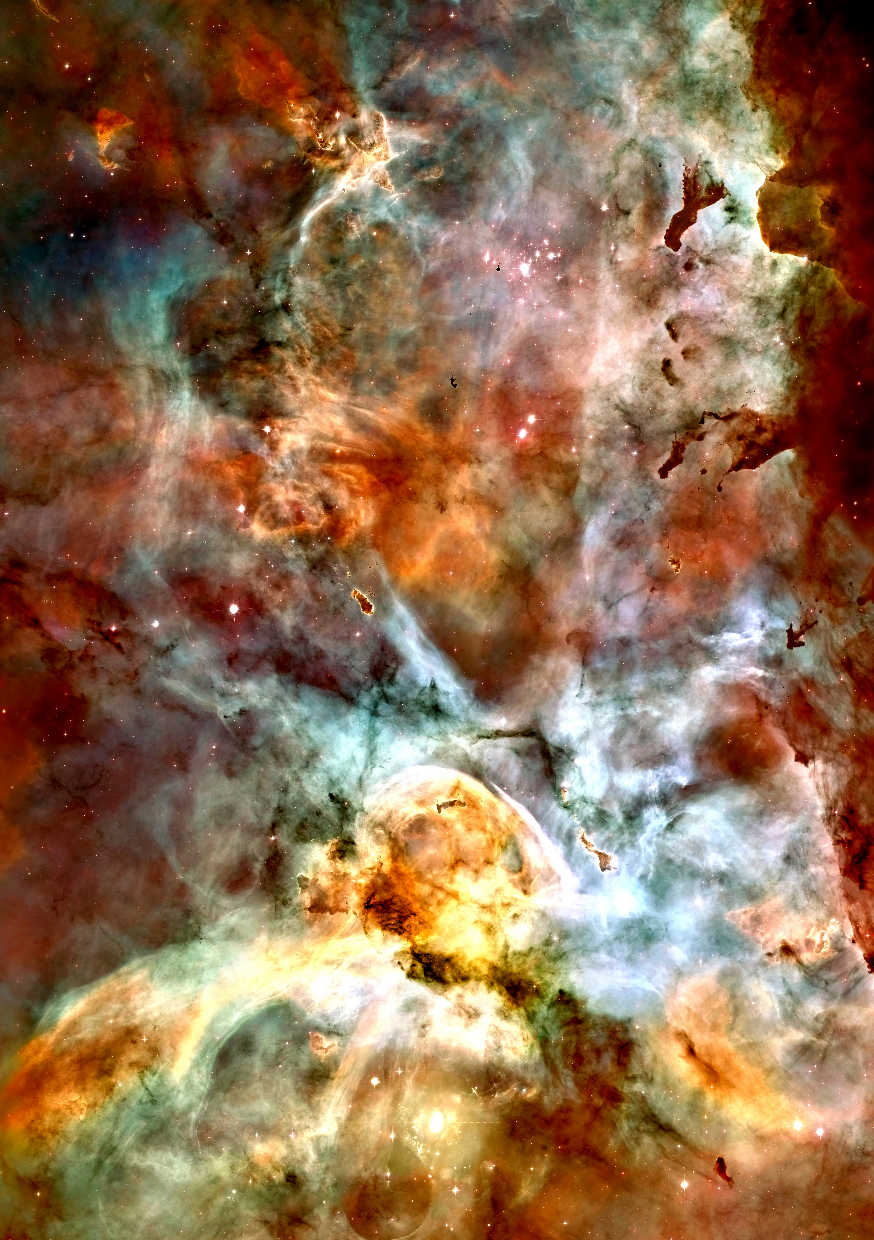
\includepdf[pages=-]{z-include-carinazoom-a5.pdf}

»Orakel!« Alexandra sprang durch die halb geöffneten Schotten hindurch und riss den Geretteten mit sich aus der Schleuse. Das Team unter Wöyt nahm es gelassen zur Kenntnis.

Tisiphöne begrüßte den etwas überforderten Neuankömmling in der Zentrale. »Willkommen an Bord. Deine Freunde dachten schon, hier liefe eine große Verschwörung.«

»Tut sie«, murrte Orakel. »Der Carinanebel ist eine riesengroße Farce. Irgendwelche Freaks haben Planeten im Schlüsselloch zerbröselt und eine Dysonsphäre hineingebaut. Weil das noch nicht großkotzig genug war, hat man außerdem eine Aldersonscheibe errichtet, die im Infrarotbereich strahlt, als wäre sie von Städten oder Fabriken durchzogen.«

Die vorläufigen Lagebeschreibungen und die Aufzeichnungsspeicher der beiden Schiffe wurden über die Warpfunkbrücke nach Örz übertragen. Spätestens jetzt gab es kein Zurück mehr: Das Geheimnis des Carinanebels war gelüftet. Die Regierung entschied sich für schonungslose Offenheit und reichte den Bericht unzensiert an die großen Verlagshäuser weiter, die daraus in unterschiedlicher literarischer Qualität für jeden Bewohner der Wirtschaftsvereinigung auch in den letzten Winkeln lesbare Nachrichten erzeugten. Es hätte nicht viel gefehlt, um einzelne Äöüzz mit dem Ausruf »Extrablatt!« durch die Straßen ziehen zu lassen.

»Wir sind hier, um uns euren Fund genauer anzusehen«, erklärte die Kommandantin. Nun betraten auch Büri, Knwrts, Tllrk und Änkäp die Zentrale und hielten skeptisch Abstand von allen anderen Anwesenden. »Willkommen an Bord der Vängefül Destrüktiön.«

»Habt ihr etwas dagegen, wenn wir eure gütigste Gastfreundschaft nicht weiter beanspruchen und mit unserem Schiff zurück in die Wirtschaftsvereinigung fliegen? Uns wird der Boden hier zu heiß.«

»Das glauben die doch selbst nicht«, witzelte Alexandra leise.

Büri verschränkte mit gespielter Empörung die Arme. »Das habe ich gehört.«

»Kein Problem«, befand Tisiphöne. »Die Kosten für den Bergungsauftrag entnehmen wir vorher dem Goldanteil der Ladung.«

»Wir haben keinen Bergungsauftrag erteilt«, widersprach Knwrts. »Wir wurden gegen unseren ausdrücklichen Willen von unserem Urlaubsort entfernt.«

Eine kurze Rekapitulation des Geschehens ergab, dass Knwrts tatsächlich nie um Hilfe gebeten hatte. In unwilliger Anerkennung, wie üblich von dem extravaganten Quartett über den Tisch gezogen worden zu sein, bat die Schiffsleitung die Ezt Indüä Kmpnö darum, sich möglichst ohne Umwege in Sicherheit zu begeben. Zwei Libürätörschiffe boten Begleitschutz für die P-2255, der tatsächlich bis zum Erreichen des Äöüzz-Einflussbereichs akzeptiert wurde. Bei Orakel und seinen Freunden, die gerade gemeinsam an einer lockeren Würfelspielpartie saßen, traf bald die Nachricht der unbeschadeten Ankunft ein. »Mit Grüßen von Nögnög Zwölf«, wiederholte yury. »Verrückte Käuze sind das.«

»Viel verrückter ist doch wohl, dass wir uns gerade schon wieder in die Hölle begeben«, fand Orakel. »Die machen kurzen Prozess mit uns.«

yury hielt den Vorstoß für alternativlos. »Wenn wir unverrichteter Dinge nach Örz zurückkehren und dort verweilen, wächst das Monster ungestört weiter. Wir müssen die Felskugel unter die Lupe nehmen, Funkkontakt zu ihren Erbauern aufnehmen und diplomatische Beziehungen herstellen.«

Acht Augen. Alexandra rückte acht Felder vor. »Einen Krieg anzetteln, meinst du.« Tack, tack, tack, tack, tack, tack, tack, tack. Eine grüne Spielfigur flog vom Feld; die Spielerin der roten Figuren durfte erneut würfeln.

Seufzend stellte yury seine Spielfigur wieder auf ein Startfeld. »Falls das ohnehin unvermeidlich ist, handelt es sich bei Angriff vermutlich um die beste Verteidigung.«

»Du kannst aber nicht mit fünfzig Schiffen ein Imperium zerlegen, und Verstärkung braucht viel zu lange zu uns.« Diesmal durfte Alexandra zehn Felder weit ziehen, konnte damit jedoch nichts anfangen. Free übernahm den Zug.

»Auch das ist vermutlich beabsichtigt. Sonst sind wir ja die Kriegstreiber.«

Alexandra verzog das Gesicht. »Weil wir weniger Schiffe schicken, als man für eine kriegerische Auseinandersetzung benötigt? Das ist keine Diplomatie, das ist Leichtsinn.«

Drei Felder: Eine rote Figur wurde von Frees blauen beiseitegeräumt und flog vom Brett. »Das hier ist jedenfalls erst einmal Sparta.«

Mit den Augen rollend reichte yury die Figur weiter. »Dreihundert ist ein historisch und politisch fragwürdiger Film voller Intoleranz und Gewalt, kein lustiges Meme für Brettspielzitate.«

»Der Vergleich hinkt sowieso«, räumte Free ein. »Wir waren es, die einen Botschafter geschickt haben.«

»Ob der Vergleich wirklich hinkt, muss sich erst zeigen.« Es konnte nicht mehr lange dauern, bis die letzte gelbe Figur ihr Zielfeld erreicht hatte. Orakel überholte Free, entging knapp einer vorbeiziehenden grünen Figur und schloss bald darauf gemütlich als Erster den Wettlauf ab.

»Gut, dass wir eine Funkbrücke dabeihaben«, fand yury. »So können wir vielleicht doch noch rechtzeitig einen Rückzugsbefehl empfangen.«

Alexandra lächelte. »Jedem von uns wurde angeboten, mit der 4-6692 oder einem Taxi nach Örz zurückzufliegen. Kostenlos. Das Angebot steht immer noch.«

Orakel schauderte ein wenig. »Vielleicht fühle ich mich hier einfach sicherer als auf Örz.« Den anderen fehlte sein direkter Eindruck von der technischen Überlegenheit der Kugelbauer. »Ich bin vor allem mitgekommen, weil Alexandra mit ihrem Flammenwerfer und Tisiphöne mit ihren Lasern dabei sind.«

»Du hattest Angst, dass man dein Taxi abfängt«, stellte Alexandra klar. »Die Nachricht von der EIK entkräftet das aber hoffentlich ein bisschen.«

»Ein bisschen, ja.« Die Gruppe schwieg sich etwa zehn Sekunden lang an, dann fuhr er fort: »Weil wir von denen ablenken. Solange wir hier sind, kommt das Monster nicht zu uns nach Hause.«

»Das ist doch wirklich tendenziös und defätistisch«, protestierte Alexandra. »Die Äöüzz sind nicht wehrlos gegenüber irgendwelchen Aliens. Weißt du eigentlich, wie viele Schiffe von der Größe der Vängefül Destrüktiön zwischen den Planeten der Vereinigung patrouillieren?«

Orakel blickte sie fragend an.

»Ich auch nicht, aber es sind viele«, behauptete sie.

»Mhm«, machte Orakel. »Ich befürchte, das Sicherheitskonzept ist ein Luftballon und basiert auf Abschreckungstechniken, die gegen das Ding im Schlüssellochnebel nicht wirksam sein werden. Es würde mich nicht wundern, wenn ein Großteil der Flotte gerade um uns herum versammelt ist.«

Diesmal blickte Alexandra erstaunt zurück.

»Und deshalb bin ich hier.«

\begin{center}
∞∞∞
\end{center}

Der vermeintliche »Luftballon« hatte zumindest Stacheln nach außen. Nachdem Orakel die Schiffsgruppe zu den Orten geführt hatte, an denen nachprüfbar Planeten verschwunden waren, stieß das Geschwader seitlich in die düstere Lemniskate hinein. Der Warpflug endete erneut zwei Lichtwochen vor den Toren, die Äöüzz wichen den Steinbrocken jedoch nicht aus. Um jederzeit ungehindert fliehen zu können, bohrten sie mit hochenergetischen Infrarotstrahlen einen breiten Tunnel durch den Staub; was bei der Verdampfung übrig blieb, wurde in den Schutzschilden in Licht verwandelt, das zu allen Seiten leuchtete.

Orakel ließ der Gedanke nicht los, dass in ihrer Abwesenheit möglicherweise die Wirtschaftsvereinigung überfallen werden konnte. Über die Warpfunkbrücke hielt er regelmäßigen Kontakt mit seinem Nachbarn und der EIK, die den Vorstoß mit einer gewissen Bewunderung, aber auch mit Kopfschütteln über seinen Leichtsinn betrachteten. Es schien fast, als wolle sich das Quartett von dem Schock im Schlüssellochnebel erholen; Tllrk schmiedete gar Ruhestandspläne. Genug Geld, um sich zur Ruhe zu setzen, hatte die Gruppe jedenfalls tatsächlich erarbeitet.

»Büri würde euch gerne folgen«, verriet Änkäp. »Aber niemals auf eigene Faust, und in Anerkennung der Bequemlichkeit, die wir gerade genießen.«

»Das wird noch früh genug sehr ungemütlich bei euch«, sendete Orakel zurück. Jede Nachricht traf mit einer Latenz von etwa einer Erdstunde ein; der Carinanebel erschwerte die Kommunikation trotz dichter Relaiskette. Um Nachrichtenverfälschungen praktisch auszuschließen, waren hohe Redundanzen und aufwendige Fehlerkorrekturverfahren notwendig.

\begin{center}
∞∞∞
\end{center}

Nach drei Wochen und gefühlt dreihundert Schachpartien standen yury, Alexandra, Free und Orakel erneut auf der Brücke und blickten in Flugrichtung »durch« die Außenmonitore hindurch auf ein massives Hindernis. Der Tunnel im Rücken war zur Beleuchtung ungeeignet und längst wieder mit Schutt gefüllt. Siebenundvierzig Scheinwerfergruppen brachten Licht ins Dunkel.

»Da drin«, bat Pägtün Twizplöt um Bestätigung, »befinden sich dreihundert Milliarden Raumschiffe, die über einer Aldersonscheibe eine Dysonsphäre umkreisen?«

»Zwischen der Scheibe und dem Felswall ist durchaus eine Menge Platz«, erklärte Orakel. »Der größte Teil der Flugobjekte befand sich dort. Was Sie auf den Videoaufzeichnungen für Raumschiffe gehalten haben, wirkte vordergründig antriebslos.«

yury lachte ohne Stimme mit uneindeutigem Gesichtsausdruck. »Was soll es schon sonst gewesen sein. Raumschrott… In Ordnung. Vielleicht.« Er holte tief Luft, ohne seine Stimmbänder zu aktivieren. »Steht das Taxi-Angebot noch.«

»Ja«, sicherte Tisiphöne sofort zu. »Jederzeit.«

»Alexandra.«

Die aptronyme Frau mit der Axt im Gürtel blickte ihn lächelnd an und zwinkerte ihm zu. »Notfalls ziehen wir das hier allein durch. Orakels Arbeit soll nicht umsonst gewesen sein.«

Der Zitierte vergaß, was er eigentlich sagen wollte, und betrachtete die Felswand erneut. Er räusperte sich und brachte langsam wieder genug Melodie zustande, um Fragen zu formulieren. »Wieso?«

»Für die Erde.«

Das war ein Argument.

»Für Örz.«

Das auch.

»Für die Milchstraße.«

Vielleicht.

»Bist du dabei?«

»Ja.«

Alexandra blickte Tisiphöne in die Augen, schmunzelte darüber, dass es dabei ein gewisses Ungleichgewicht gab, und zeigte auf die Bildschirme. »Eigentlich dürfte die Kugel gar nicht existieren, weil Verschiebungen aus der Grundposition sich sofort selbst verstärken. Das Gebilde ist ungefähr so stabil positioniert wie eine Murmel auf einer Bleistiftmine.«

Das hatte yury seinen Kollegen zuvor erklärt. Orakel war es nicht aufgefallen. Nicht einmal die Bordcomputer hatten ihn darauf hingewiesen; Tisiphöne und Twizplöt hatten sich keine Gedanken darüber gemacht. Offenbar wurde er tatsächlich gebraucht.

»Wir könnten es darauf ankommen lassen und die Kugel ein bisschen anstupsen.« Free grinste. Bevor jemand auf die Idee kommen konnte, dafür ernsthaft eine Lagebesprechung einzuberufen, bat er darum, die Idee vorerst zu den Akten und nach Örz zu legen. »Das wäre undiplomatisch.«

»Der eigentliche Plan ist auch nicht gerade das Gelbe vom Ei«, wandte yury ein. »Nur, weil niemand öffnet, bohrt man sich ja nicht mit Lasern durch die Haustür.«

»Und weil es unfreundlich ist, die Tür aufzubohren, stößt man stattdessen das Haus um, ja?« Lökül Sjävärüty stand einige Meter entfernt an einem Kontrollpult und schnippte belustigt mit seinen Fingern darauf herum.

Twizplöt fand, die Rolle der Milliarden Flugobjekte sei damit auch geklärt: Es handele sich um Zeltheringe.

yury runzelte die Stirn. »›Fishy‹, würden unsere Engländer sagen, ist dieser Erklärungsversuch. ›Somehow fishy.‹ Nicht ganz astrein.«

Twizplöt gab zu, man könne sich die Situation beliebig schönreden. Es sei Zeit, Orakels ersten Eindruck mit Messdaten und Fakten zu vervollständigen. Das war das Stichwort.

\begin{center}
∞∞∞
\end{center}

Ein großes, einen Kilometer durchmessendes Loch wurde in die Wand gedampft. Bei dieser Breite wirkte der Durchbruch kaum noch wie ein Tunnel. Selbst durch diesen Umstand und Vorwissen abgeschwächt traf der Anblick des Kugelinneren jedoch jeden, der in diesem Moment einen Blick auf einen Außenbildschirm warf.

Türd Üpnön fand als Erster die Sprache wieder. Tiefe Bedrückung belastete sein Herz. »Man fühlt sich wirklich wie eine Fliege, die sich auf einem Erdbeerkuchen niederlässt.«

»Ohne Zuschauer«, riet Orakel. »Das entspricht meiner Beobachtung vor der Flucht. Scheinbar kümmert sich niemand um uns.«

»Wenn wir jetzt fliehen und auf einem Planeten landen, werden wir vielleicht ebenfalls abgeschossen. Unter Umständen gehört das hier zum Begrüßungsritual.« Alexandra umfasste den Bildschirm mit beiden Händen, als müsse sie Displayreflexionen durch Sonnenstrahlen verhindern.

Tisiphöne kniff alle drei Augen zusammen. »Das wird aus zwei Gründen nicht geschehen: Erstens genügt der Treibstoff für einen Direktflug nach Örz, zweitens besteht derzeit keine Fluchtabsicht.« Die Aldersonscheibe schien Städte voll kühlbedürftiger Anlagen zu beinhalten, strahlte dementsprechend infrarot, zeigte im sichtbaren Bereich jedoch nur eine ziemlich glatte Felsoberfläche.

»Dort wird etwas produziert«, beurteilte Rüff Tüff das Gesehene. »Man möge sich kurz vorstellen, unsere Wirtschaftsvereinigung wäre nicht auf Planeten verteilt, sondern über eine solche Scheibe. Genug Platz für die Lebewesen bestünde jedenfalls.«

»Sie meinen, die Energieausgabe wäre vergleichbar?«, fragte Free. Er bemühte sich, eine grobe Vorstellung des irdischen Stromverbrauchs auf das Sternenreich der Äöüzz hochzurechnen. Ihm fehlten jedoch Daten, um auch nur Größenordnungen zu vergleichen.

»Die Energieabgabe dieses Sterns dort beträgt circa sieben hoch einunddreißig Watt«, las Tüff von einem Bildschirm ab. Er schlug einige Zahlen in einer Wissensdatenbank nach.

yury warf ein: »Auf Örs hat man gerade Fissionskraftwerke, die klassische ›Kernkraft‹, als Energiequelle überwunden. Die Abgabeleistung eines solchen Kraftwerks ist aber eine Vergleichsgröße, mit der wir hier vielleicht kurz arbeiten können. Man spricht da von ungefähr einem Gigawatt.«

Nun wurde mit Zahlen und Einheiten jongliert. »Gut, wir nutzen Gigawatt als Vergleichsgröße. Ein Kernkraftwerk, ein Gigawatt. Zwei Kernkraftwerke, zwei Gigawatt. Euer Heimatplanet, dreitausend Gigawatt.«

»Wir haben nie im Leben dreitausend Kernkraftwerke«, protestierte Orakel.

»Stimmt, da ist jede andere Form der Stromerzeugung mit inbegriffen. Nicht enthalten hingegen ist der Energieverbrauch von Stahlwerken, die noch mit Kohle befeuert werden, und ähnliche veraltete Vorgänger des elektrischen Stroms.«

Das brachte Orakel zum Grübeln. »Autos mit Benzin?«

Alexandra lächelte. »Ja, aber die gibt es kaum noch. Seit die Menschen wissen, dass es auch andere bewohnte Planeten gibt, streben sie gemeinsam den Fortschritt an.«

»Wie viel Strom wird denn zum Beispiel auf Örz verbraucht?«, erkundigte sich Free.

Hierzu konnte Extän Jämäjän einige Informationen liefern. »Auf Örz findet praktisch keine Primär- oder Sekundärwirtschaft statt. Da laufen ein paar Server, da werden Supermärkte beleuchtet, Unterhaltungselektronik wird mit ein paar Watt versorgt und Touristenfolien werden aufgeladen.«

Mit gewisser Skepsis entgegnete Free, die ›paar Server‹ fräßen auf der Erde eine gewaltige Menge Leistung, die~– von Lüftungs- und Beleuchtungsanteilen abgesehen~– vollständig als Wärme abgegeben werde.

»Das liegt an eurer ineffizienten Prozessortechnik«, fand Jämäjän. »Wir können mit einem Gigawatt vermutlich sämtliche Rechner der Erde ersetzen.« Er blickte auf Tüffs Bildschirm. »Ihr nutzt allein für den Betrieb des Internets das Sechzigfache davon.«

»Auf Örz wird weniger Strom verbraucht als auf der Erde«, schloss yury. »Ich meine, ich hätte etwas von einer halben Million Äöüzz gehört, die in der Hauptstadt lebt. Der größte private Arbeitgeber ist Sümsün, dicht gefolgt von Äppöl und IGLS.«

»Die halbe Million kommt hin«, bestätigte Tüff. »Für den ganzen Planeten.«

yurys Kollegen waren überrascht; Alexandra bat ihn um Bestätigung. »Auf ganz Örz leben weniger Menschen als im hessischen Frankfurt?«

Er nickte. »Frankfurt ist doch ein passender Vergleich. Wenn man die gesamte automatisierbare Wirtschaftsleistung von Robotern erledigen lässt, werden zur Verwaltung einer Welthauptstadt auch nicht mehr Menschen benötigt.«

Damit ließ sich Orakel jedoch nicht abspeisen. »Sümsün allein hat doch bestimmt mehr als hunderttausend Mitarbeiter.«

»Nicht auf Örz«, erklärte Üpnön. »Die Produktion wurde auf Industriesysteme ausgelagert, die Entwicklung erfolgt dezentral. Auf dem Hauptplaneten sind Behörden und Forschungsinstitute damit beschäftigt, ein tausend Lichtjahre durchmessendes Sternenreich verwaltbar zu halten. Echter Energieverbrauch findet bei der Exekutive statt, die sich größtenteils im All aufhält. Wer für die imperiale Polizei arbeitet, verbringt seine Freizeit auf Monden und Zwergplaneten, um jederzeit ohne großen Wasserstoffverlust einsatzbereit zu sein. Das Militär landet gar nicht erst; Tisiphöne betritt vielleicht einmal im Jahr einen Planeten.«

»Aber Älföns Ögnöwäk…«

Tisiphöne grinste verlegen und nahm Üpnön die Antwort vorweg. »Hat dir schon einmal jemand gesagt, dass du wenig über die Äöüzz weißt?«

»Tatsächlich, ja«, stammelte Orakel. »Ich glaube, wir belassen es dabei.«

\begin{center}
∞∞∞
\end{center}

Die Wirtschaftsvereinigung der Äöüzz umfasste ungefähr zweitausend bewohnte Planetensysteme. Keines davon war so dicht bevölkert wie die Erde, keines davon nutzte so viel Strom. Zusammen mit dem Raumschiffverkehr kamen fünf Millionen Gigawatt zustande, eine beachtliche Leistung.

Planeten und Raumschiffe wandelten die Energie in Wärme und Licht um. Man sprach auch von »Exergie«, um die Energie zu bezeichnen, die beispielsweise in Form von Wasserstoff oder Sonnenlicht noch für die Äöüzz nutzbar war. Industrieprozesse, Rechenzentren, Raumschiffe und letztendlich auch jedes Lebewesen gaben dieselbe Energie als »Anergie« ins Weltall ab: Überschüssige Infrarotstrahlung, der eine oder andere verfehlte Laserstrahl, Funkwellen und das Helium, das beim Fusionskraftwerkbetrieb anfiel.

Im Gegensatz zum lockeren Sternenhaufen der Äöüzz war der »dysonal ausgebeutete G-Stern« von zwei Sphären umgeben: Eine Dyson-Sphäre, die einen beachtlichen Teil des Sonnenlichts aufnahm, und die äußere große Felsschale. Letztere stellte ein Hitzeproblem dar: Der Stern lieferte konstant hundertfünfzig Yottawatt, die in Wärme umgewandelt oder als Licht freigelassen werden mussten. Den Äöüzz wurde schnell bewusst, dass es ein Ventil geben musste, das außerhalb ihrer Sichtweite lag.

Kommandantin Tisiphöne, ihr Stellvertreter Sjävärüty, die Navigatorinnen Twizplöt und Pässtrü, Alexandra und Orakel waren damit beschäftigt, sich äußerst vorsichtig mit der Raumschiffgruppe durch das Schalenloch zu bewegen, einen Überblick vom Innenleben zu erhalten und Funkkontakt zur Scheibenbevölkerung aufzunehmen. Der physikalisch-elektrisch fokussierte Teil der Besatzung hatte sich an einem Nebentisch niedergelassen und fachsimpelte über mögliche Erklärungen.

Mit den Worten »Das kann man nicht speichern, indem man Wasser aufspaltet. So viel Wasser gibt es im ganzen Carinanebel nicht« schob Rüff Tüff eine Theorie ins Abseits. yury und Free räumten ein, dass die Idee möglicherweise so absurd wie das gesamte Felskonstrukt war, aber Tüff hatte seine Erklärung noch nicht beendet. Er steigerte sich in einen Vergleich hinein: »Das flüssige Wasser auf Örz in allen Flüssen und Seen zusammen«, schlug er beim Reden nach, »sind ungefähr zwei mal sieben hoch zwanzig Liter. Ein Liter wiegt bei vier Grad Celsius ziemlich genau ein Kilogramm, so habt ihr das ursprünglich definiert. Für uns sind es 348 Örztempz und 2,228 ISG.«

\iathought{Die Umrechnung hätte er sich sparen können}, dachte yury amüsiert. \iathought{Wir kennen die Faktoren inzwischen. Ein Örztemp ist die thermodynamische Temperatur des Tripelpunktes des Wassers geteilt durch 7³. Ein InterStällär Gräm ist die Masse von 3 mal 7 hoch 29 Silicium-28-Atomen. Man könnte da ein paar Nachkommastellen ergänzen.} Die Wassermenge und die nachfolgende Hochrechnung weckten allerdings sein Interesse.

»Aus einem Kilogramm Wasser wird, sehr optimistisch betrachtet, ein achtel Kilogramm Wasserstoff. Dass Meerwasser vollkommen versalzen ist und die Effizienz pro Liter mindert, sei einmal dahingestellt.«

Free fragte sich, ob es praktikabel war, die Ozeane auf manchen Planeten vollständig zu entsalzen. Örz war zu siebzig Prozent mit Land bedeckt, hatte durch seine zentrale Wetterkontrolle und große Auffangsysteme jedoch keine Süßwasserprobleme.

Nach einer kurzen Recherche mit weiteren Daten gewappnet, fuhr Tüff fort: »Die Hochtemperaturelektrolyse von Wasserstoff in Sternwärmekraftwerken benötigt üblicherweise um die sechzig Kilowattstunden pro Kilogramm Wasserstoff. Dabei herrschen Temperaturen von über achthundert Grad Celsius. Wir nehmen stattdessen als Gedankenspiel an, dass die Elektrolyse perfektioniert wurde, sodass wir die gesamte Strahlungsleistung ohne Wärmeverluste hineinstecken können. Dann werden nur noch vierzig Kilowattstunden benötigt.«

yury sprang ein: »Auf der Erde können also bis zu sechs Trillionen Gigawattstunden durch Wasserstoffelektrolyse gespeichert werden.«

»Sechs komma vier, ja. Die Einheit ›Trillionen Gigawattstunden‹ entspricht Yottawattstunden. Diese Kapazität ist nach zweieinhalb Minuten eurer Zeitrechnung erschöpft, wenn man die gesamte Leistung des Sterns hineinpumpt.«

»Das heißt«, überschlug yury, »man benötigt pro Jahr mindestens zweihunderttausend Erdmengen Wasser. Selbst, wenn jeder Stern im Carinanebel von einem erdähnlichen Planeten umkreist würde, wäre der Vorrat nach weniger als einem Jahr aufgebraucht.«

»Es ist nicht ausgeschlossen, dass die Erbauer der Dyson-Sphäre einen beachtlichen Teil der gewonnenen Energie irgendwie zwischenspeichern. Der Rest muss irgendwann nach draußen abgegeben werden. Mit Spiegeln vielleicht?«

»Mit überdimensionalen Lasern«, schlug Jämäjän vor.

Von Tüff gab es Beifall: »Dann wäre es auch gar nicht überraschend, dass wir mit hoch entwickelter Lasertechnologie angegriffen wurden. Die Idee gefällt mir.« Auch die anderen bekundeten Zustimmung.

»Das ist ineffizient und unpraktikabel«, gab Üpnön hingegen zu bedenken. »Mit Spiegeln und einem Austrittsloch ist es irgendwie machbar. Mit Lasern erzeugt man beim Abkühlvorgang zu viel Hitze.« Es ergebe keinen erkennbaren Sinn, das Licht zuerst in Strom und anschließend wieder in Licht umzuwandeln.

»Vielleicht haben wir etwas übersehen«, fürchtete Free. »Der Stern da gibt gar nicht so viel Leistung her, wie der Bordcomputer berechnet hat.«

Das sah Tüff anders. »Die Erbauer der Riesenstruktur mögen über gewaltige technische Mittel verfügen, aber Physik ist Physik.«

»Mit den aktuellen Daten über die Felskugel und den Stern, rein physikalisch betrachtet, müsste Orakel bereits beim Durchbruch eine Katastrophe ausgelöst haben. Spätestens dann geriet das Konstrukt nämlich ins Ungleichgewicht.«

»Dafür gibt es doch die Heringe«, warf Jämäjän ein. »Ich verstehe noch nicht, wie die funktionieren, aber sie sind da.«

»Klar«, erlaubte sich yury sanften Spott. »Die funktionieren mit Traktorstrahlen.«

»Es gibt keine–«

yury blickte ihn verschmitzt an.

»Himmel, wir müssen doch nicht immer alles sofort erklären können«, wich Jämäjän verzweifelt aus.

»Das wäre eigentlich der Anspruch gewesen, doch, doch.« Dann ließ er ab; er wollte den Äöüzz nicht in die Ecke drängen.

Tüff blickte sich um; sein Blick haftete an Orakel, der sich eine warme Erbsendose aus einem Automaten geholt hatte. »Wie ist denn die Lage da draußen?«

»Joa«, schmatzte der, »die wollen nicht mit uns reden.«

»Haben sie das gesagt?«

Orakel leerte in aller Ruhe die Dose und kaute zu Ende, bevor er die Spannung fallen ließ: »Nee, eben nicht.«

»Niemand antwortet auf unsere Funksprüche. Inzwischen haben wir auf Warp- und Normalfunkfrequenzen mit allen uns bekannten Modulationsverfahren so breit mit elektromagnetischen Wellen um uns geworfen, dass wir von jedem Empfänger innerhalb der Kugel eine genervte Bitte um Ruhe erwartet hätten. Das Licht braucht sieben Örzkläks von hier bis ans andere Ende der Schale. Die sind mehrfach vergangen.« Twizplöt starrte über den Stern hinweg auf die schwach beleuchtete Felsinnenwand.

»Wir sollten noch eine Weile hier im Außenbereich verweilen«, beschloss Tisiphöne. »Es wäre nicht angebracht, ohne Einladung weiter vorzudringen.«

Alexandra schmunzelte. \iathought{Es war niemals angebracht, diese Kugel aufzubrechen. Wie lange möchtest du warten, werte Äöüzz, und worauf? Das Wetter wird vom Zuschauen nicht besser.}

Obwohl das alles unausgesprochen blieb, blickte Tisiphöne ihr grinsend in die Augen. »Die Evaluation eures Sondereinsatzes steht noch aus. Eine Befürwortung zukünftiger Einsätze ist derzeit nicht möglich.«

Wettstarren für zwei Minuten~– Tisiphöne gab auf und blinzelte im Kreis. »Untersteh dich.« Belustigt wandte sie sich wieder ihrem Bildschirm zu.

»Free, du kannst doch bestimmt eine Liste der Beiboote abrufen.«

Dieser Wunsch stieß auf ein gewisses Unbehagen. »Kann ich das?«, fragte er yury.

yury bemühte sich um Neutralität. »Schon irgendwie. Technisch und so.«

»Eher nicht so, irgendwie«, fand Lökül Sjävärüty. »Eher gar nicht so.«

»Doch, doch«, bestätigte Free dann in Alexandras Richtung, an Sjävärüty vorbei. »Ich habe dir die Tabelle mal geschickt.«

»Was wird hier gespielt?«, fragte der Vizekommandant pikiert.

»Tennis«, erklärte yury. »Dä böl iz in ür kürt.«

Es schien Zeit für ein Machtwort zu sein; mangels Stellungnahme von Tisiphöne übernahm Sjävärüty die leidvolle Aufgabe. »Wir warten. Mindestens einen ganzen Örzröt, um zu sehen, ob es eine Reaktion auf unsere Nachrichten gibt. Je nach Staatsform ist es durchaus angebracht, den Kontaktierten selbst für die erste Antwort genügend Bedenk- und Debattierzeit zu lassen, bevor man mit der Tür ins Haus fällt.«

\iathought{Wir haben die Tür pulverisiert, laut ›Hallo‹ gerufen und wollen jetzt einen Tag lang auf der Schwelle stehen bleiben}, fand Alexandra, aber niemand außer ihr schien an der Anweisung etwas auszusetzen zu haben. Ein wenig mit schwachem Trotz und leicht gekränktem Stolz begab sie sich mit den irdischen Kollegen in den Gemeinschaftsraum der Gästekabinen. Dort tippte sie auf ihrem Smartphone herum und war für einige Stunden schwer ansprechbar.

\begin{center}
∞∞∞
\end{center}

Das zähe Schweigen der Angerufenen strapazierte seit sechzehn Stunden die Geduld der Schiffsgäste. Die Felskugel bewegte sich von keiner Seite auf ihren Stern zu, die Aldersonscheibe strahlte von örtlich unveränderten Feldern sehr weiträumig und mit beständiger Intensität infrarot umher, der eine oder andere Felsklumpen fiel durch das Loch hindurch auf die Schutzschirme der Vindikätören. Ein paar kleine Steinchen verirrten sich durch den Schiffspulk hindurch und stürzten der Dysonsphäre entgegen~– niemand traute sich, mit Lasern hinterherzuschießen. Es war davon auszugehen, dass Sicherheitsvorkehrungen eine Beschädigung durch solch kleine Fremdkörper verhinderten.

Dann ertönte der Schiffsalarm.

Alexandra war als Erste auf den Beinen, stolperte in ihre Kabine, riss aus Schubladen und offenen Ablageorten alle greifbaren Verteidigungsmittel, ließ sich luftdicht von ihrem Raumanzug abschirmen und kehrte zurück zu ihren Freunden. Orakel, yury und Free hatten ihre Helme ebenfalls geschlossen und das Schott geöffnet; die Gruppe trat geschlossen auf den Gang hinaus und lief mit ernster Eile fast im Gleichschritt der Kommandobrücke entgegen. Tiefe Sirenentöne und bewegungsunabhängige Vollbeleuchtung aller Laufwege vermittelten den noch ihr Frühstück verarbeitenden Menschen, dass der Arbeitstag uhrzeitunabhängig angebrochen war. Jede Form von Hektik fehlte jedoch: Die umhergehenden Offiziere strahlten professionelle Besonnenheit aus.

»Guten Morgen«, wünschte Tisiphöne. »Wie ihr eventuell geahnt habt, dient der Schiffsalarm nicht zur Benachrichtigung über eine friedliche Kontaktaufnahme.«

»Guten Morgen«, entgegnete Alexandra freundlich. »Werden auf den Außenbildschirmen historische Aufzeichnungen dargestellt, ist der Frequenzfärber deaktiviert oder sind wir gerade trotz des Alarms und fehlenden Funkkontakts außer Gefahr?«

»Es gibt Funkkontakt«, erklärte Tisiphöne.

yury zählte gedanklich an den Fingern die verbleibenden Möglichkeiten ab. »Haben wir eine Kriegserklärung erhalten? Für, öh, einen Laserangriff in ein paar Sekunden?«

Die Kommandantin wies mit der Hand auf ihre Navigatorinnen und bat diese stumm um eine Erklärung. Es war Tängänä Pässtrü, die letztendlich das Wort ergriff.

»Wir haben über die Funkbrücke die Nachricht erhalten, dass mehrere Planeten im Außenbereich der Wirtschaftsvereinigung, darunter alle unbewohnten Felswelten des Nögnög-Systems, gerade von breitfrequenten Multilasern buchstäblich \emph{zerschnitten} werden. Die dafür eingesetzten Raumschiffe sind jeweils kleiner als 3087 Kubikmeter; pro Planet sind etwa 343 bis 2401 dieser Maschinen im Einsatz.«

Twizplöt reservierte sich einen der großen Bildschirme auf Augenhöhe und stellte darauf eine Skizze der Eindringlinge dar.

»Was tut das Militär?«, fragte Orakel.

»Panisch seine schlecht positionierten Truppen verlegen«, mutmaßte yury. »Man kann davon ausgehen, dass die Schiffe mit Überlichtgeschwindigkeit unbemerkt hinter den Außenposten aufgetaucht sind.«

Orakel, der das vollständige Verschwinden mehrerer Planeten im Carinanebel nachvollzogen hatte, sah den nächsten Schritt bereits kommen: »Man wird die Planetenstücke abtransportieren und zur Reparatur der Felskugel nutzen. Das ist so direkt als Reaktion auf unser Eindringen ersichtlich, dass es für jedes raumfahrende Lebewesen als härtestmögliche Erwiderung ohne echte Eskalation wirken muss. Auge um Auge, Zahn um Zahn. Wir können mit Glück davon ausgehen, dass wir keinen wassergefüllten Lebensraum beschädigt haben; die Reaktion wäre sonst sicherlich der Abbau von Wasserwelten.«

»Wir müssen aus zwei Gründen von hier verschwinden«, stellte yury fest. »Erstens besteht eindeutig Interesse daran, das Loch zu schließen, notfalls hinter uns. Zweitens sind wir hier genau so unerwünscht wie die Schneideschiffe in unseren Systemen. Wenn wir die Kugel verlassen, lässt man vielleicht ebenfalls von Nögnög Neun und Co. ab.«

Tisiphöne wirkte unentschlossen. Ihre Aufgabe lag eigentlich darin, Licht in dieses Dunkel zu bringen; das stille Sternenreich in der Kugel stellte ansonsten eine dauerhafte Gefahr für alle anderen Lebewesen der Galaxis dar. Dass nach Gutdünken Planeten in bewohnten Systemen zerstört wurden, ließ sich nicht als Reaktion rechtfertigen und nicht ohne Aufgabe der eigenen Gebietshoheit hinnehmen.

Free ließ sich im direkten Gespräch mit der zweiten Navigatorin ein paar Daten bestätigen. »Der Fokus der Angreifer liegt auf den unbewohnten Nögnög-Felswelten?«

»Scheinbar, ja«, berichtete Pässtrü. Sie öffnete eine vereinfachte Karte, auf der die angegriffenen Planetensysteme als rote Sterne sichtbar waren. Jeder betroffene Planet war statisch wie an einer Kette neben seinem Hauptstern aufgereiht. Nögnög war eindeutig am stärksten betroffen, und ein Blick auf die umliegenden Systeme zeigte dem Betrachter, dass das nicht an einem Mangel ähnlicher Felswelten in der Region lag.

»Die Ezt Indüä Kmpnö befand sich zuletzt noch im Nögnög-System«, erinnerte sich Sjävärüty. »Es war vor allem auch ihr Ankunftsziel.«

Pässtrü und Free, die sein Herantreten nicht bemerkt hatten, blickten ihn kurz irritiert an und nahmen dann den Faden auf.

»Vielleicht wurde die P-2255 auf ihrer Rückreise verfolgt. Man weiß nie, wie ›sichtbar‹ die Äöüzz für Außenstehende sind. Die Menschen auf Örs haben das Imperium nicht selbst bemerkt, obwohl seit Jahrtausenden zahlreiche Raumschiffbewegungen im Ara-Nebel stattfinden. Nun hat man jedenfalls unsere Außenplaneten entdeckt.« Da es um das Trio herum still geworden war, hallten Pässtrüs Worte durch den Raum.

yury wandte sich an die Kommandantin. »Tisiphöne, Sie haben uns unter anderem als Berater hinzugezogen«, leitete er seine Bitte vorsichtig ein. »Nun wird vermutlich eine gewisse Uneinigkeit in der gesamten Besatzung darüber herrschen, wie hier idealerweise vorzugehen ist. Es ist in vielerlei Hinsicht nicht unbegründet, dass es sich letztendlich um eine Kommandoentscheidung handelt, die Ihnen niemand abnimmt. Als Sie den Präsidenten informiert haben, wird eine ähnliche Situation vorgelegen haben.« Er biss sich auf die Zunge. Der Präsident hatte den Auftrag trotz aller Gefahren genehmigt. Die kaputte Argumentationslinie ließ sich nicht mehr zurücknehmen. Es wirkte dann auch überhaupt nicht mehr, dass er mit zur Flucht mahnenden Worten fortfuhr~– Tisiphöne betrachtete Flucht als ein finales, unwiderrufliches Scheitern der Mission.

»Vielen Dank für das Feedback«, bedankte sich Tisiphöne sanft. Sie gab noch keine Entscheidung bekannt; das Schiff verblieb an Ort und Stelle.

\begin{center}
∞∞∞
\end{center}

Über Nögnög III war die Hölle los. Der atmosphärelose Planet wurde von allen Seiten mit weißen Laserbündeln beschossen, das Gestein schmolz, verdampfte sofort, verteilte sich neben der Schnittstelle. Bis zum flüssigen Kern des Planeten hindurch schnitt sich Laser für Laser, das wertvollste Gut des Planetensystems und einen entscheidenden Stabilisator für alle Planetenbahnen wie eine Pizza behandelnd. Als die ersten Militärschiffe eintrafen, um dem Treiben ein Ende zu bereiten, wurden alle eingehenden Funksprüche ignoriert. Irgendwann wurde es den Äöüzz zu bunt und der inzwischen mit der Situation überforderte Vitällö befahl den Einsatz von Lasern und Kanonen gegen die Eindringlinge. Dies war der Moment, in dem Tisiphöne den wahren Wert von Feedback zu schätzen lernte.

\ialoudspeaker{»Wir werden beschossen.«}

Selten meldete sich der Bordcomputer des Kriegsschiffs zu Wort. Die Vängefül Destrüktiön war ein in professioneller Arbeitsteilung gesteuerter Koloss, kein Einzelpilotenflugzeug. Was an Diagnosedaten anfiel, wurde auf den Bildschirmen der Techniker dargestellt. Es gab nur wenige Nachrichten, die so bedeutungsvoll waren, dass eine Mitteilung über die allgemeinen Bordlautsprecher für die gesamte Besatzung sinnvoll war, und zumeist genügte die Zeit, um solche Durchsagen von der Kommandantin durchführen zu lassen. Diese Nachricht hingegen war zeitkritisch und für alle bestimmt.

\ialoudspeaker{»Der unmittelbare Verlust der Rümpünt Tränsfürör und der Vökäl Ägitätör ist passiv nicht vermeidbar. Das Laserfeuer auf die nächsten Angreifer wurde eröffnet.«}

»Feuer einstellen«, rief yury entsetzt. »Sofort das Feuer einstellen!«

Rüff Tüff schlug mit einer Faust kräftig auf den Besprechungstisch. Er erhob sich, durch den internen Eingriffsversuch nicht weniger erbost als über den äußeren Angriff. Die Umstehenden hatten Schwierigkeiten, alle Einzelheiten der Tischszene bei gleichzeitiger Betrachtung der Außenbildschirme zu erfassen. »Die Örsmenschen aus der Zentrale. Zuschauen kann man aus jedem Raum.«

»Seid ihr des vollkommenen Wahnsinns?«, schrie yury in die Runde. Etwa ein Dutzend Offiziere trat Person für Person hinzu und baute eine gewisse Drohkulisse auf. Die Gastfreundschaft war abrupt überstrapaziert worden. Draußen zerplatzte der äußere Schutzschirm der Vökäl Ägitätör; fünf der »Zeltheringe« vergingen im Kreuzfeuer der Äöüzz. »Das Örz-Militär hat vermutlich gerade die Eindringlinge im Nögnög-System beschossen. Die Nachricht fehlt uns, den Angreifern aber nicht. Vielleicht hat man die bessere Warpfunktechnik, was weiß ich. Seid ihr bescheuert, das eskalieren zu lassen? Wisst ihr, was gleich mit Nögnög Zwölf geschieht?«

»\emph{Das} wäre allerdings eine Eskalation«, erwiderte Tüff kalt. »Wir schießen nicht auf bewohnte Systeme. Kannst du mich hingegen noch einmal daran erinnern, wessen Raumschiff über dem violetten Planeten zu Bruch gegangen ist?«

Fest davon überzeugt, dass gerade eine Katastrophe eingeleitet worden war, aber ohne kurzfristig parates Gegenargument zur Quelle der Eskalation starrte yury auf den Bildschirm eines Örztöps am Besprechungstisch. Fünfzehn, sechzehn Explosionsreste. Die üblicherweise durch Sauerstoff verursachte schwarze Färbung der Wrackteile fehlte. Ohne über seine unmittelbare Umgebung nachzudenken, trat yury an das Gerät heran und machte Anstalten, die Ansicht mit einer Fingergeste zu vergrößern. Das kam in Unkenntnis seiner Intention nicht gut bei den Umstehenden an und führte vor der Displayberührung zu einem physischen Rauswurf.

\begin{center}
∞∞∞
\end{center}

yury tobte innerlich; nach außen machte er aus dem Bewusstsein seiner Hilflosigkeit keinen Hehl. Mit stumpfem Blick wohnte er auf dem Gästesofa der Zerstörung hunderter kleiner Laserschiffe bei, die zuvor für reine Befestigungsanker gehalten worden waren.

Alexandra hatte einen nüchterneren Blick auf die Situation. »Die Explosionen sind recht stark für solche kleinen Schiffe, nicht wahr?«

Die Explosionen hatten eine solche Leuchtkraft, dass die Rümpünt Tränsfürör zum vorläufigen Ende des Gefechts ihren Außenschirm ohne direkten Beschuss verlor. Die elektromagnetischen Wellen, die beim letzten Aufblitzen der Angreifer die Umgebung traktierten, brachten gewissermaßen das Fass zum Überlaufen. Bei großen Reaktoren war das ein erwartbares Ergebnis, und auch gemessen an der Feuerkraft der Zerstörten war der Schaden nicht überproportional. Alexandra hatte im Katzenpfotennebel schon einmal einen Widersacher im Plutoniumfeuer seines Kollegen vergehen lassen. Nur ließ sich im hier vorgefundenen Schiffsvolumen~– weniger als hundert Kubikmeter~– kein Plutoniumreaktor unterbringen, der sich in dieser Heftigkeit aus dem Dienst verabschiedete.

»An Bord der Schiffe scheint es keinen Sauerstoff in nennenswerter Dosierung gegeben zu haben«, erwähnte yury. Er griff nach dem Örztöp und zeigte seinen Freunden die Beobachtung, die von den großen virtuellen Außenfenstern bereits verschwunden war. »Es ist kein Ruß zu erkennen.«

»Siliziumwesen!«, rief Free begeistert aus. »Das wäre eine absolute Sensation.«

»Immer langsam«, beschwichtigte ihn Orakel. »Was du da siehst, ist ein Roboterschiff, das bis an den Rand mit Plutonium gefüllt war, um im Zerstörungsfall maximalen Umgebungsschaden zu hinterlassen. Eine autonome Weltraummine, ein verachtenswertes Instrument zur Grenzkontrolle.«

»Das müsste sich mit einer Spektralanalyse nachweisen lassen.« Alexandra beauftragte beim Zentralcomputer eine Untersuchung der Wellen, die auf den Außensensoren der Vängefül Destrüktiön eingetroffen waren. Sie erhielt sofort überproportionale Rechenkapazität für ihr Vorhaben, was yury richtigerweise als sanftes Wiedergutmachungsangebot der Bordführung interpretierte. »Wir sind mit Priorität 110 unterwegs, zehn Punkte unter üblichen Benutzerprozessen.«

»Je niedriger die Prioritätsnummer ist, desto mehr Rechenzeit erhalten wir pro Takt«, erklärte Free. »Wie man hier nachsehen kann…« Er ließ sich eine Baumansicht der Systemprozesse anzeigen, soweit dies einem Gast möglich war. »…wurde die Wurzel unseres Benutzerzugangs mit der Bezeichnung ›wichtige Berechnungen‹ markiert. Wenn wir es darauf anlegten, könnten wir die Kaffeemaschine in der Zentrale zum Stillstand bringen, weil wir ›wichtiger‹ sind und den Strom dringender benötigen.«

»Es war kein Plutonium im Spiel«, las Alexandra ein Zwischenergebnis vor. »Auch kein anderes Transactinoid war an den Explosionen beteiligt.«

yury runzelte die Stirn. »Das ist nicht die einzige Merkwürdigkeit. Die Schiffe verfügten über Triebwerke und kräftige Laser. Die beiden Äöüzz-Schiffe waren ernsthaft von einem Schildverlust bedroht. Wie passt solche Technik in eine Kugel mit knapp sechs Metern Durchmesser?«

»Alles, was man braucht, ist ein Miniatur-Synchrotron. Uns fehlt jede Vorstellung davon, wie diese Wesen mit elektromagnetischen Wellen jonglieren können. Vielleicht gibt es etwas Besseres als supraleitende Elektromagneten, um Teilchen in runde Bahnen zu zwängen.« Free zuckte mit den Schultern.

»Und die Explosion?«

»Vollständige Fusion von Wasserstoff, der den Rest der Kugel gefüllt hat. Hitze aus den beeindruckenden Superlasern, vielleicht Lithiumhydrid als Energiespeicher. Orakels Erklärung klingt doch ansonsten recht plausibel.«

Das sah der Zentralcomputer anders. Alexandra ließ die Berechnung mehrfach mit unterschiedlichen Annahmen wiederholen, bat um detaillierte Simulationen und ließ tatsächlich einige Offiziere länger als üblich auf ihre Getränke warten.

\begin{center}
∞∞∞
\end{center}

Die Schiffsführung verfolgte den Anstieg der Prozessorlast mit neugierigem Interesse. Die Technikerin Bäsh Hötröp präsentierte ihren faszinierten Kollegen die von Alexandra veranlassten Befehle und deren Ausgabe.

Jämäjän stieß einen erstaunten Pfiff aus. »Das würde allerdings den enormen Exergieverbrauch ganz ohne ein Ventil erklären.«

»Es gibt wohl kaum einen ineffizienteren Weg, um Energie zu speichern. Für die verbleibende Hitze bräuchte man sehr wohl ein Ventil«, korrigierte ihn Sjävärüty.

»Vielleicht haben die Erbauer dieses Reichs die Energieeffizienz optimiert. Das Energie-für-Volumen-Verhältnis ist jedenfalls unschlagbar. Und was das Anergieventil angeht, ist Infrarotstrahlung doch ganz nützlich. Sie wird besser reflektiert als sichtbares Licht und kann mit Metallspiegeln besser in eine Richtung gelenkt werden.«

»Wohin, Lieutenant?«

»Das weiß ich nicht. Jedenfalls klären sich gerade viele andere Fragen gleichzeitig. Der Energiebedarf, die Feuerkraft der winzigen Raumschiffe und die Wucht der Explosionen. Leider scheitern unsere Kommunikationsversuche. Vielleicht ist das alles ein bitteres Missverständnis und wir haben großartige Verbündete gefunden.«

Eine Nachricht von Örz traf ein; Tisiphöne gab diese in einem Rundspruch an die anderen Schiffe weiter: »Der Angriff in und um Nögnög wurde abgewehrt. Das Parlament hat den Kriegsfall ausgerufen; Älföns Ögnöwäk verwaltet als Flottenadmiral das weitere Vorgehen.« Abseits des Mikrofons, nur an die Anwesenden gerichtet, fügte sie hinzu: »Man war ähnlich verwundert wie wir über die Energiedichte der zerstörten Schiffe, und man geht gerade derselben Hypothese nach.«


\chapter{Eskalation}

Zum Betrieb von Warpantrieben, selbst modernster Exemplare, war stets eine geringe Menge Antimaterie erforderlich. Ein gut gesicherter Vorrat von Antiwasserstoff, an Bord der 4-6692 etwa stecknadelkopfgroß, deckte auf jedem Äöüzz-Schiff für ein Vielfaches der Schiffslebensdauer den Bedarf. Insofern waren Antimaterie und die damit erzeugbaren Auslöschungsreaktionen den Äöüzz durchaus ein Begriff; es gab Industrieplaneten, auf denen hauptsächlich Antimateriekapseln für Raumschiffe hergestellt wurden.

Ein Gramm Materie entsprach etwa 25 Gigawattstunden Energie~– genug, um zweitausend Erdfamilienhaushalte für ein Erdjahr mit Strom zu versorgen. Wenn Wasserstoff auf Antiwasserstoff traf, wurde die Energie freigesetzt. Die Teilchen löschten sich gegenseitig aus.

Als Energie\emph{quelle} war Antimaterie ungeeignet, da sie im Universum nicht nutzbar natürlich vorkam und somit auch nicht eingesammelt werden konnte. Zur Nutzung als Energie\emph{speicher} für mobile Kraftwerke fehlte den Äöüzz nur die nötige Herstellungseffizienz. In den vorhandenen Teilchenbeschleunigern wurden Protonen auf das 0,9994-Fache der Lichtgeschwindigkeit beschleunigt und auf Iridiumstäbe geschossen, wodurch Antiteilchen entstanden. Die so gewonnenen Antiprotonen wurden mit Magneten aussortiert und durch große Ansammlungen von Xenonatomen am Weiterflug gehindert. Der seltene, kaum forcierbare Zusammenstoß der Antiprotonen mit Xenon ließ Positronen entstehen, die mit viel Glück so nah an einem Antiproton entstanden, dass sie mit diesem eine Bindung zum Antiwasserstoff eingingen. Für den winzigen Antimateriebedarf von Warpantrieben war dieses Vorgehen ein notwendiges Übel, für alle anderen wirtschaftlichen Anwendungsfälle schied es aus.

Nun zeichnete sich ab, dass die Wesen, die eine planetensystemgroße Felsschale um eine Aldersonscheibe und eine Dysonsphäre gebaut hatten, letztere zur Produktion von Antimaterie nutzten. Hierfür musste ein physikalisches Verfahren zum Einsatz kommen, das den Äöüzz bisher unbekannt war. Womöglich beherbergte die Aldersonscheibe einen großen Beschleunigerring, aber das allein genügte nicht, um die vergleichsweise geringe Wärmestrahlung des Konstrukts zu begründen.

\begin{center}
∞∞∞
\end{center}

Über Nögnög IX explodierten zweitausend antimateriegeladene Roboterschiffe. Die anschließend nicht mehr mit Lasern auf den Planeten gerichtete, sondern unkontrolliert in alle Richtungen weisende Strahlung degradierte zwei mittelgroße Militärschiffe zu verglühten Metallklumpen und führte auf diese Weise zu den ersten Verlusten unter den Äöüzz. Anschließende Bergungsaktionen gestalteten sich schwierig: Der Planet war knapp einer Zerstückelung entgangen und entwickelte tektonische Aktivität, die man für längst kontrolliert und eingedämmt gehalten hatte. Magma brach aus dem Boden hervor, Vulkane entstanden. Der wirtschaftliche Aufschwung des Schwarzfelskonzerns erfuhr nach Jahrhunderten seinen ersten katastrophalen Dämpfer, kam im Zuge von Reparaturarbeiten zum Erliegen und fiel hinter die Tourismuseinnahmen zurück. Diese waren zeitgleich über jede Prognose hinweg durch die Skalendecke gebrochen und wurden für eine Weile hauptsächlich logarithmisch dargestellt, damit die Diagramme lesbar blieben. Nögnög, das gefährlichste Planetensystem der Wirtschaftsvereinigung, wenig besuchswerter Schauplatz des absehbaren Untergangs, frei zugänglich für jeden Raumschiffbesitzer durch gelebten Liberalismus. Apokalypsetourismus, der die Ezt Indüä Kmpnö vergrämte und nach Frzn trieb, das Heimatsystem der beiden bunten Käfer.

Unterdessen bemühte Tisiphöne sich eindringlich um Kommunikation, die über das Zerstören von Planeten und Raumschiffen hinausging und mit weniger Kollateralschäden verbunden war. Es dämmerte ihr, dass ihre Verständigungsversuche nicht durch fehlende Technik auf der Empfängerseite scheiterten; die gezielte Zerstörung des Warpfunkmoduls der 4-6692 war bereits ein erstes Anzeichen für äußerst fortgeschrittene Funkinterpretation gewesen. Warpfunknachrichten gewissermaßen »abzufangen«, war eine Kunst, die man auf Örz selbst kaum beherrschte. Der Funk bewegte sich mit Überlichtgeschwindigkeit zu einem klar definierten Ziel; es gab kein bekanntes zuverlässiges Mittel, um die Nachricht auf ihrem Weg überhaupt zu bemerken.

»Mit Ungeziefer verhandelt man nicht«, formulierte Sjävärüty überspitzt die Lage. »Man zeigt Grenzen, setzt diese durch und rückt nicht von seinem Standpunkt ab. Dass Verhandlungsversuche stattfinden, ignoriert man mangels Interesse an allem, was angeboten werden kann.«

»Dann säßen wir nicht seit drei Tagen unbehelligt im Einflugloch«, fand Pägtün Twizplöt. »Die Grenze haben wir überschritten, ein Durchsetzen wurde mehr oder weniger ernsthaft versucht, und nun starrt man sich gegenseitig an.«

»Wir starren nicht«, korrigierte Tisiphöne, »wir betteln um Anhörung. Ziemlich laut sogar, und beharrlich wie Roboter.«

Wie Roboter.

Pässtrü rang mit Argumentlosigkeit, wollte sich aber eine Ahnung von der Seele reden. »Dass sie Roboterschiffe bauen können, haben die Leute hier bewiesen.«

»Mhm?«

»Vielleicht wird das ganze System von Robotern verwaltet.«

»Unter wessen Auftrag wäre das dann?«, fragte Tisiphöne leicht belustigt. »Galaktische Illuminaten?«

Ein wenig gekränkt über die klare Zurückweisung ihrer Idee verzichtete Pässtrü auf eine Antwort und tippte schweigend auf ihrer Pulttastatur vor sich hin.

\begin{center}
∞∞∞
\end{center}

yury lief im Kreis um den Spieltisch herum, während Free mit subjektivem Erfolg versuchte, Orakel das Schachspielen beizubringen. Irgendwann waren der Gruppe die Kartenspiele ausgegangen und Orakel hatte verhaltenes Interesse an dem königlichen Wettkampf gezeigt. Klassische schwarze und weiße Figuren besetzten gleichfarbige Felder. Alexandra beobachtete die Szene vom Sofa aus, blickte aber eher durch das Zimmer hindurch, als ihren Blick zu fokussieren.

»Es hilft alles nichts«, sagte Alexandra zögerlich. »Wir müssen den Elefanten im Raum ansprechen, auch wenn wir uns damit unbeliebt machen. Es ist unsere Aufgabe als externe Berater, auch Perspektiven einzubringen, die man hier nicht hören möchte.«

»Ich halte nicht viel von externen Beratern, die ihre Perspektiven einbringen möchten«, erwiderte yury, »und die Äöüzz sicherlich auch nicht. Man holt sich ›Berater‹, weil man Auflagen erfüllen muss, Zertifikate braucht, klaffende Unfähigkeit mit einem Pflaster zudecken will und zu viel Geld besitzt.«

»Oder?«

»Und.«

Alexandra schüttelte langsam den Kopf. »Wir kosten nichts außer Nerven.«

Das stimmte irgendwie. »Was ich sagen wollte: Wir sind genau so lange erwünscht, wie wir die vorherrschende Meinung bekräftigen.«

»Meinst du denn nicht«, fragte sie sanft, »dass die Äöüzz inzwischen tief in ihrem Inneren den gleichen Verdacht entwickeln? Hier wird nicht nur Geschichte geschrieben~– hier wird Geschichte ausgegraben. Wir können nicht vernünftig arbeiten, wenn wir die Hintergründe nicht kennen, also müssen wir diese erfragen. Man zwingt uns doch geradezu, das zu tun.«

yury schwieg betrübt. Links neben ihm zog Orakel mit einem Turm schräg, weil dieser die einzige verfügbare Figur war, nachdem er dreißig Züge lang vermieden hatte, sich die Blöße des Vergessenhabens zu geben. Free lächelte und ersetzte einige seiner Figuren durch weiße Äquivalente. Nun konnte der Turm bestimmungsgemäß ziehen, ohne sich in Gefahr zu begeben. Orakel hingegen war nun noch mehr verwirrt: Der Farbtausch von Figuren gehörte also auch zu den vergessenen Regeln. Bemüht, starke Züge zu spielen, wandelte er seinen König in eine schwarze Dame um. Free war die nächsten fünf Minuten damit beschäftigt, das Missverständnis beidseitig aufzuklären.

»Traust du dir das zu?«, fragte yury mit ernsten Bedenken so freundlich wie möglich.

»Nein«, antworteten alle drei gleichzeitig. »Aber ich gehe trotzdem«, fügte Alexandra hinzu. »Vorsichtig, langsam, zurückhaltend und ohne Axt.«

»Dann könnte es funktionieren.«

Alexandra öffnete das Schott, trat auf den Gang hinaus, blickte auf das Schachbrett zurück und winkte kurz, bevor sie mit gesenktem Blick das Tor schloss. Immerhin hatte Orakel wieder einen König auf dem Brett und bewegte diesen regelkonform; auch ein blindes Huhn fand mal ein Korn. Oder ein Imperium im Schlüssellochnebel, natürlich.

Es kam jedoch nie zu dem vorsichtig anvisierten Gespräch. Noch während Alexandra über den Gang schritt und im Voraus über ihre Wortwahl nachdachte, gellte der Schiffsalarm auf und verstummte für eine Schreckensnachricht von Tisiphöne.

\ialoudspeaker{»Raumanzüge anlegen und verschließen. Jedes Besatzungsmitglied hält sich in geschlossener Raumkleidung zum Außeneinsatz bereit.«}

Durch einen schnellen Knopfdruck ließ sich Alexandra mit einem luftdichten Anzug mit Schutzschildgenerator umgeben.

\ialoudspeaker{»Mehrere Millionen Laserschiffe, Kugeln mit einem Durchmesser von sechzehn Metern, sind über den unbewohnten Felswelten des Nögnög-Systems erschienen und haben sofort das Feuer eröffnet. In Einzelfällen befanden sich unsere Patrouillen zwischen den Eindringlingen und den Planeten. Sie wurden genau wie das kaum wirksame Gegenfeuer der Äöüzz ignoriert. Die Planeten existieren vermutlich bereits nicht mehr. Für uns besteht derzeit keine unmittelbare Gefahr, aber wir beginnen jetzt mit einem Gegenschlag. Ziel ist die Dysonsphäre, die von außen möglicherweise nicht so strahlungsfest wie gegenüber dem Stern ist. Wir haben den Auftrag, Planetentechnologie einzusetzen, um die Sphäre zu einem in unserem Ermessen liegenden Grad zu beschädigen.«}

»Also, um sie letztendlich zu zerstören«, murmelte Alexandra und sprinte energisch auf das nächste Brückentor zu. Die davor positionierte Offizierin übte verhaltenen Protest.

»Sie benötigen eine Einladung, –«

»Nein.«

Das Schott öffnete sich vor ihr und schloss sich, während Alexandra bereits stehend am Besprechungstisch Platz nahm. Eilig wurde ihr ein Stuhl gereicht.

Stumm verschaffte sich Alexandra einen Überblick über das galaktische Geschehen. Sie platzierte einige Notizztettel und Eilmeldungen auf ihrem Abschnitt der elektronischen Tischoberfläche. Ein Eindruck von Dreidimensionalität wurde vermittelt, als ihr der Platz auf der Ebene ausging: Zwei Notizzettel überlappten sich, ohne dass der untere Zettel ganz unlesbar wurde. Tängänä Pässtrü schob einen Stapel virtuellen Anschauungsmaterials zu ihr herüber; ihr linker Sitznachbar Sjävärüty gab ihr einen Teil seiner Fläche ab. Er hatte es längst aufgegeben, sich über die Gepflogenheiten der Erdmenschen zu echauffieren, wurde aber stets aufs Neue von deren Impulsivität überrascht.

»Dankeschön«, flüsterte Alexandra, in Gedanken vertieft. Pägtün Twizplöt und Rüff Tüff diskutierten über das weitere Vorgehen; ab und zu warf Tisiphöne ihre Bedenken oder ihre Genehmigung ein. »Ihr habt das Ventil inzwischen gefunden?«

»Unzählige Kandidaten, die sich als Ventile nutzen ließen«, erklärte Pässtrü mit gedämpfter Stimme. Sie stand auf und stellte sich zwischen Alexandra und Tisiphöne an den Tisch. »Die Felskugel ist nicht ganz dicht. Es gibt dauerhaft beschattete Bereiche, die bei näherer Betrachtung kleine Löcher enthalten~– Tunnel für scharf gebündeltes Licht. Und wenn sie dafür genutzt werden, möchte man nicht der Vogel sein, der durch den Lichtstrahl fliegt.«

Alexandra stellte sich ein irdisches Sonnenwärmekraftwerk vor und winkte dankend ab. »Spiegel oder Laser?«

»Vermutlich Spiegel. Laser sind nicht erforderlich und weniger effizient.«

Beide nickten nach kurzem Überlegen und durchstöberten den Dokumentenstapel.

Tisiphöne bat kurzfristig um Aufmerksamkeit. »Die Felsplaneten des Nögnög-Systems werden gerade in Stücken abtransportiert. Die kleinen Raumschiffe haben sich daran verankert und verfügen über genügend Kraftreserven, um sie auf relativistische Geschwindigkeit zu beschleunigen und in den Warpraum mitzunehmen. Die Äöüzz haben ferngesteuerte Schiffe in die Flugbahn gelegt, die aber ihre Kollision mit den Riesenbrocken keine Sekunde überstanden haben. Der Schrott ist mitgerissen worden und fällt mangels Verankerung bei der ersten Warpraumabbremsung irgendwo aus der Blase. Den findet man nie wieder.«

»Unzerstörbar sind die Schiffe aber erwiesenermaßen nicht. Konnten wir den Angreifern keine Verluste zufügen?«, fragte Alexandra schockiert.

»Tausende. Zehntausende. Was sind schon solche Zahlen gegen Millionen Angreifer.«

Free, Orakel und~– zögerlicher~– yury betraten die Zentrale. Letzterer war in stiller Trauer versunken und wohnte den Unterhaltungen passiv bei. Ab und zu sah er Abbildungen des Grauens, kniff seine Augen zusammen und öffnete den Mund, als stöhne er vor Schmerz. Das Trio nahm abseits des Besprechungstisches auf Stühlen in einem Viertelkreis Platz, Alexandra seitlich zugewandt.

Tisiphöne fuhr fort: »Es handelt sich durchweg um Roboterschiffe; das Militär hat da recht geringe Hemmungen, größtmöglichen Schaden zu verursachen. Planetenraketen kamen allerdings nicht zum Einsatz. Einerseits, weil der Kampf über unseren eigenen Planeten stattfand, und andererseits, damit wir einen Überraschungseffekt nutzen können. Die Fähigkeit, kurzzeitig schwarze Löcher im All zu erzeugen, wird man nämlich kaum von uns erwarten.«

Orakel rang um Verständnis. Er glaubte, ein absurdes Bild im Kopf zu haben: »Millionen Schiffe, die sich irgendwo außerhalb der Monsterkugel befanden, sind zusammengekommen, um das zu veranstalten.«

Die Herkunft der Schiffe war bei näherer Überlegung ein Mysterium. Free sah Orakel nachdenklich an. »Wir haben doch die Schiffsbewegungen in diesem System im Blick. Die Kugel hat einen Innendurchmesser von gut zehneinhalb Lichtminuten und ist einigermaßen überschaubar. Alles hier drin ist beleuchtet, entweder direkt durch den Stern oder indirekt durch die beleuchteten Felsen. Von einem Abzug der Millionen Raumschiffe haben wir nichts mitbekommen?«

»Die Raumschiffe kamen nicht aus dieser Kugel«, bestätigte Pässtrü.

Das gab Orakel den Mut, sich mit seinen Überlegungen in Richtung des Tisches zu wenden. »Wenn sich allein im Inneren dieser Kugel mehrere hundert Milliarden Kleinstschiffe befinden und nun Millionen größere Schiffe innerhalb von drei Örztagen für einen Angriff bei NGC 6188 mobil gemacht werden konnten, fehlen uns ein paar Puzzleteile.«

»Zum Beispiel?«, fragte die zweite Navigatorin interessiert nach.

»Wer schickt die Befehle? Das ist ja kein Guerillakampf. Irgendjemand hat festgestellt, dass wir in der Felskugel stören, und hat einen sehr genau bemessenen Gegenschlag geradezu chirurgisch durchgeführt.«

»Die Befehle werden wohl aus der Scheibe kommen. Genauigkeiten zum Aufbau der Scheibenstädte sind uns nicht bekannt.«

»Eigentlich«, mischte sich Tüff ein, »ist uns nicht einmal bekannt, ob Städte existieren, und in welcher Form.«

Pässtrü zog den Mund schräg. Das war ihr natürlich bewusst, aber sie hatte es in der kurzen Erklärung bewusst vernachlässigt. Die Ungewissheit über grundlegende Parameter der fremden Strukturen bedrückte sie.

\begin{center}
∞∞∞
\end{center}

Nach einer gefühlten Ewigkeit stand das weitere Vorgehen fest. Tisiphöne verkündete den Beschluss als Rundfunkspruch und über alle Bordlautsprecher.

»Wir haben uns einen Zielpunkt auf der Aldersonscheibe ausgesucht, der wärmer als seine Umgebung ist. Auf dem Weg dorthin kommen wir ›zufällig‹ sehr nah an der Dysonsphäre vorbei. Wenn der Abstand so gering ist, dass selbst ein antimateriegefülltes Raumschiff an der Innenseite der großen Felsschale nicht mehr schnell genug beschleunigen kann, um einen kurzen Warpflug einzuleiten und sich dazwischenzuwerfen, feuern wir mit neununddreißig Neunundvierzigsteln unseres Planetenraketenvorrats auf die Metallsphäre.«

Das war allerdings noch nicht alles. Der zweite Teil der Nachricht traf die neben ihr sitzenden Menschen unvorbereitet. »Die Zivilisten yury, Orakel, Alexandra und Free werden vor Beginn der Angriffshandlungen mit der 4-6692 nach Örz eskortiert.«

yury schaltete schnell. Das Mikrofon war knapp ausgeschaltet, als er mit ernsten Bedenken vorstieß. »Kommandantin Tisiphöne, Vizekommandant Lökül Sjävärüty, Sie bringen Örz in die Gefahr, die über Nögnög bereits hereingebrochen ist. Wir bezweifeln das dauerhafte Verschonen bewohnter Welten durch die Antimaterieschiffe, besonders falls Sie tatsächlich die Dysonsphäre beschädigen.«

»Möchten Sie stattdessen nach Nögnög gebracht werden?«, fragte die für die Transportmission verantwortliche Hauptnavigatorin verwundert und gutherzig. Tisiphöne war sich ihrer Entscheidung hingegen sehr bewusst und intervenierte, bevor es zu Missverständnissen kam.

»Örz ist gesichert, und für eure Verteidigung ist mehr als ausreichend gesorgt.«

yury blinzelte.

»Das soll genügen. Alles Weitere erfahrt ihr, sobald ihr am Zielort eingetroffen seid. Ich danke euch, auch im Namen der gesamten Besatzung, für eure Rolle in diesem riesigen galaktischen Schachspiel. Es ist nun Zeit für euch, das Zentrum zu verlassen und euch auf die hinteren Reihen zurückzuziehen.«

\cleardoubleevenpage

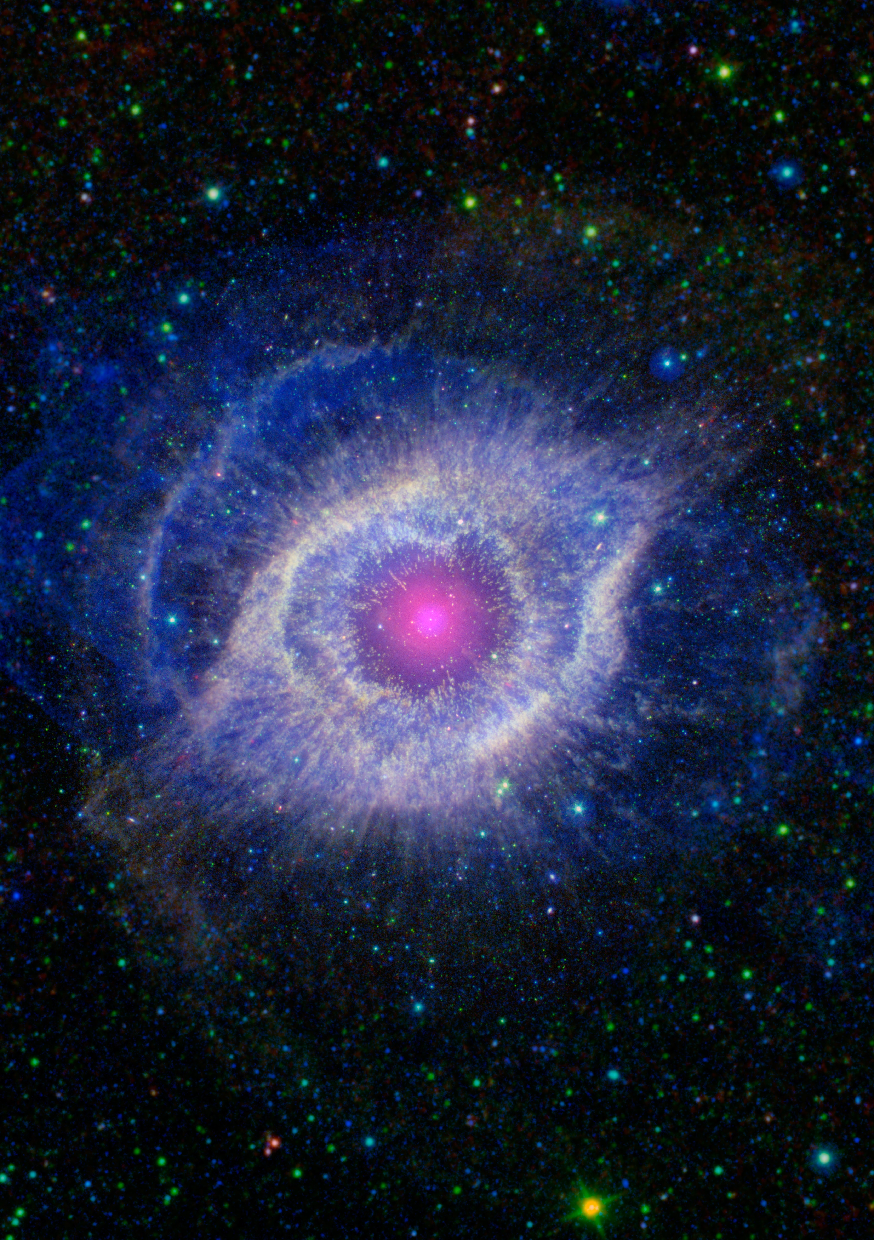
\includepdf[pages=-]{z-include-helixnebula-a5.pdf}

\chapter{Berichte aus dem Helixnebel}

\section{Level 11: Ruhe vor dem Sturm}

Regen tropfte sanft gegen die Zeltwände. Manche Tropfen verirrten sich durch den Dachschlitz in den Wohnraum und tropften auf die Glut, zischten im Übergang zum Dampf und holten Floating Island sanft aus seinen Träumen.

Es war der Morgen des fünften Novembers, ein Samstag, der schon vor Sonnenaufgang mit wechselhaftem Wetter aufwartete und den in einer virtuellen Naturwelt gefangenen Ex-Diktator darauf aufmerksam machte, dass es irgendwo ein Spielziel gab. Flucht ins Weltall lautete die Devise~– ein Jetpack hatte man ihm bereits geschenkt. Nun sollte ein Sturm aufziehen, sinnbildlich oder buchstäblich, und das Zelt wirkte nicht besonders sturmfest. Seufzend erhob sich Island von seiner Isoliermatte, knabberte an einer Möhre und wechselte seine Kleidung. Dann begab er sich nach draußen, blickte sich im Morgengrauen um, packte im Zelt seine Sachen zusammen und lief »zielwärts« dem Äquator entgegen.

Erneut nutzte Island den Trick, drei hintereinanderliegende Bäume anzupeilen, um geradeaus zu laufen. Sobald er am ersten Baum angekommen war, suchte er nach dem nächsten Exemplar, sodass immer zwei Bäume »aktiv« eine schnurgerade Linie bildeten. Als Ausgangspunkt dienten die durch Rindenschläge markierten Orientierungsbäume vom Vortag.

\section{Level 12: Die Mondlichtung}

\iathought{Zeit für eine Mittagspause}, fand Floating Island. Die Sonne stand inzwischen hoch am Himmel, was durch das dichte Nadeldach kaum auffiel. Er legte eine Rast auf einem umgefallenen Baumstamm ein, der sich als bequeme Picknickbank eignete. Ein kleiner nach oben abstehender Ast wurde zur Seite geknickt, damit es genug Platz für den Rucksack gab. Auf dem Speiseplan standen heute fertige Nahrungspakete zum Aufwärmen in Plastik. Island befreite einen Teil des Bodens von frisch gefallenen Nadeln, errichtete aus kleinen Ästen einen Holzstapel und faltete darauf einen kleinen Titankocher auseinander. Anschließend entfachte er mit Streichhölzern ein Feuer und erhitzte Wasser in einem kleinen Topf. Als das Wasser kochte, riss er zwei Essenspackungen auf und kippte den Topfinhalt in das Nahrungspulver. Ein paar Minuten später löffelte er genüsslich Gemüseravioli und Reis, eine kleine Portion Kartoffeln und einen konservierten Obstsalat. Zum Abschluss genoss er einige Hartkekse und ein Stück Zartbitterschokolade.

Frisch gestärkt, den Kocher und den Abfall wieder im Rucksack tragend, setzte Island seine Reise fort. Langsam gewöhnte er sich an die Natur.

\begin{center}
∞∞∞
\end{center}

Die Suche nach einem dritten Baum gestaltete sich unerwartet schwer, da nun eine große Lichtung im Weg lag. Kreisrund, etwa hundert Meter durchmessend, lag eine gemähte Wiese ohne Zusatzbewuchs mitten im Wald. Als Island einen Fuß auf die Lichtung setzte, versank der Planet in Dunkelheit.

Erschrocken zog Island seinen Fuß zurück~– blendend hell schien die Sonne wieder von oben herab. Ein Fuß auf die Lichtung: Dunkelheit. Zwei Füße: Es blieb dunkel. Wo vorher die Sonne durch Nadeln zu sehen war, schien nun der Vollmond auf die Lichtung. Erst, als beide Füße die Lichtung wieder verlassen hatten, kehrte der Tag zurück.

»Was soll das? Wo ist die Bedienungsanleitung dafür?«, fragte Island. Er blickte sich um und rümpfte die Nase. Als er erneut die Lichtung betrat, fiel ihm ein blaues Leuchten auf: Zwischen einigen Grashalmen lag ein quadratischer, handgroßer Plastikzettel, der im Mondlicht schimmerte. Instinktiv nahm Island ihn aus der Lichtung heraus, um ihn im Sonnenlicht lesen zu können, doch im Sonnenlicht wirkte er durchsichtig und unbeschriftet. Es half auch nicht, ihn über die Lichtung zu halten, ohne diese selbst zu betreten. Seufzend lief er nach vorne in das Mondlicht und las im Halbdunkel eine antike Weisheit.

\noindent \parbox{\textwidth}{ \vspace{3ex} \hrule \vspace{3ex}

\textbf{Die Wirksamkeit des Negativen}

\iaquote{Dreißig Speichen umgeben eine Nabe:\\
In ihrem Nichts besteht des Wagens Werk.\\
Man höhlet Ton und bildet ihn zu Töpfen:\\
In ihrem Nichts besteht der Töpfe Werk.\\
Man gräbt Türen und Fenster, damit die Kammer werde:\\
In ihrem Nichts besteht der Kammer Werk.}

\iaquote{Darum: Was ist, dient zum Besitz.\\
Was nicht ist, dient zum Werk.}

\vspace{3ex} \hrule \vspace{3ex} }

»Das sagt mir… nichts.« Floating Island war enttäuscht. Diese ewige Philosophie raubte ihm irgendwann noch den Verstand. Er interpretierte die Zeilen schließlich so, dass sich in der Mitte der Lichtung irgendetwas Tolles befinden musste, und lief geradeaus auf das Zentrum des Kreises zu.

Nach einigen Minuten Laufen bemerkte Island, dass etwas nicht stimmen konnte. Er befand sich vielleicht auf der Hälfte des Weges, doch der Weg war gewachsen. Hinter ihm, um ihn herum, überall war diese riesige Lichtung; mindestens hundert, vielleicht zweihundert Meter lagen hinter ihm. Verwirrt erhöhte er sein Tempo, um das scheinbar ebenso nahe Lichtungszentrum zu erreichen. Er achtete stärker auf seine Umgebung, sah die Bäume in seinem Rücken davondriften, schien auf ein kilometerweit entferntes Ziel zuzulaufen und fand dennoch, dass das Gras unter seinen Füßen sich ganz normal verhielt. Er beschloss, ein Stück im Kreis um das Zentrum zu laufen, und das funktionierte anscheinend problemlos. Wirklich beurteilen ließ es sich durch die Rotationssymmetrie der Lichtung kaum, also brach Island die Symmetrie und trat mit den Fußspitzen das Gras kaputt, während er lief. Es dauerte eine gefühlte Ewigkeit, bis er wieder am Ausgangspunkt ankam, aber damit war zumindest bestätigt: Bewegungen senkrecht zum Radius wurden nicht von dem Effekt erfasst.

Langsam begriff Floating Island, welchen Gesetzen die Lichtung folgte. Er lief zurück nach außen und erreichte sein Ziel eher, als er aus der Mitte heraus geschätzt hatte. Dann nutzte er das Smartphone seines Vorgängers als Stoppuhr, joggte zum Takt eines eingängigen Liedes exakt eine Minute lang in den Kreis hinein und benötigte auch genau diese Zeit für den Rückweg. Der Lichtungseffekt wirkte wie eine Lupe, fast wie die Darstellung schwarzer Löcher in manchen Science-Fiction-Filmen. Da Island eigentlich keine Science-Fiction-Filme sah, ärgerte er sich über den Hinweis. \iathought{Ich würde das Rätsel gerne allein lösen}, dachte er, und er wusste genau, dass er sich später dafür verfluchen würde. Dafür war das Erfolgsgefühl umso größer, als weitere Experimente nach seinen Vorstellungen verliefen.

Gerade Lauflinien zwischen zwei Randpunkten der Lichtung wurden zu Kurven. Es war im Nadelwald nicht ganz einfach nachzuvollziehen, aber hundert zurückgelegte Meter außerhalb der Lichtung ließen sich beliebig in die Länge ziehen, je mehr man davon ins Innere der Lichtung verlegte. Den Abschluss der Experimente bildete ein halbstündiger Lauf am Zentrum vorbei, dessen Mittelpunkt genau zwischen dem Zentrum und dem Rand lag. Bis zur Hälfte des Weges wuchs die Lichtung, danach schrumpfte sie wieder. Das Zentrum selbst war unerreichbar, weil die Lichtung sich bei Zentrumsannäherung bis ins Unendliche vergrößerte.

Konsequent lehnte Floating Island es ab, sich weiter mit der Mondlichtung zu beschäftigen. \iathought{Solche merkwürdigen Spielereien muss man ignorieren, um im Spiel voranzukommen}, dachte er; keinen weiteren Blick schenkte er dem mystischen Konstrukt. Ungefähr auf seinem alten Pfad fand er drei neue Bäume und spazierte frohgemut davon.

\begin{center}
∞∞∞
\end{center}

Dem Spielleiter schien seine Entscheidung nicht zu gefallen. Wer sonst konnte dafür verantwortlich sein, dass der Wald in der Ferne rot leuchtete und glomm? Wer hatte~– hastige Blicke in alle Himmelsrichtungen~– einen lückenlosen Kreis des Feuers geschaffen?

Nun gab es zwei Optionen: Das Jetpack enthielt noch genug Treibstoff, um den Waldbrand zu überfliegen. Es war jedoch absehbar, dass weitere Maßnahmen existierten, um auch diesen Fluchtweg abzuschneiden. Floating Island wollte lieber das Zentrum der Mondlichtung erreichen, als diese Maßnahmen kennenzulernen. Der Waldbrand war wohl als sanfter Wink mit dem Zaunpfahl zu verstehen, und als Vorgeschmack. Niemandem war an einer Steigerung gelegen.

Daher kehrte der Abenteurer zurück zur Mondlichtung und durchsuchte seinen Rucksack nach etwas, das er darin entdeckt und ohne Vorstellung von dessen Nützlichkeit mitgenommen hatte. Es gab vielleicht einen Weg, diese Lichtung an der Nase herumzuführen.

Aus fünf Seilen wurden hundert Meter stümperhaft zusammengeknotetes Schummelwerkzeug. Eine Seite wurde um den nächsten Baumstamm gebunden, die andere Seite transportierte Island am Innenrand der Lichtung auf die gegenüberliegende Seite. Wie er vermutete hatte, hing die Lichtungsgröße ausschließlich von seiner eigenen Position ab, sodass das Seil ohne weitere Verlängerung das Zentrum durchquerte. Island bewegte das Seil hin und her, in der Hoffnung, irgendetwas Unsichtbares in der Mitte zu treffen. Er wurde in dieser Hinsicht enttäuscht.

Eine zweite Idee sollte seine letzte in dieser Existenzebene sein. Der Plan war effektiv, doch dessen Konsequenzen mussten ihn buchstäblich verbrennen. In Unkenntnis dieses Umstands tat Floating Island etwas, das yury oder Free an seiner Stelle um jeden Preis vermieden hätten: Er fesselte seine Handgelenke in einer Schlinge und trat dem Zentrum entgegen, in der naiven Hoffnung, einen genialen Einfall gehabt zu haben.

Ein Ruck ging durch das Seil. Was wie Tauziehen begann, entwickelte sich nach fünf Sekunden zu dem Gefühl, als Hund an einer Leine mitgerissen zu werden. Noch immer war Island dazu entschlossen, das Experiment durchzuziehen, und lehnte sich nach hinten vom Seil weg. Der Baum am anderen Ende der Lichtung blieb indessen an seinem Platz, und auch die Länge des Seils blieb konstant. Starke Kräfte zerrten an dem Gefesselten und rissen tiefe Furchen in die Erde, wo die Sohlen seiner Schuhe ihm nicht genug Halt gegen den Seilzug boten.

Es dauerte nicht lange, bis die Beschleunigung ihn vornüber kippen und auf den Knien rutschen ließ. Optisch trennten ihn nur noch zehn Meter von seinem Ziel, praktisch jedoch die Unendlichkeit. Er legte mehrere Kilometer im Matsch zurück; hinter ihm verschwand seine Herkunft im Horizont. Die Lichtung übertraf bald tausende Fußballfelder an Fläche; der Wind pfiff unangenehm an seinen Ohren vorbei. Auf das Gefühl, durch den Morast gezogen zu werden, folgten Armschmerzen und Flugangst. Der Luftwiderstand und die Geschwindigkeit erfüllten den Albtraum: Island hob vom Boden ab. Er flog durch die Luft dem Lichtungszentrum entgegen, noch immer an das unveränderte Seil gefesselt und von diesem durch die Atmosphäre geschleift. Hitze gab ihm zu verstehen, dass er im Physikunterricht einige Grundlagen allzu theoretisch betrachtet hatte und dass Flugzeugflügel wahrlich nicht um ihre Aufgabe zu beneiden waren. »Immerhin bekomme ich durch den Luftzug keine Erkältung«, wusste Island. Ein schwacher Trost bei einer Umgebungstemperatur von fünfzig Grad Celsius.

Sechzig, siebzig. \iathought{Finnland!}, schoss es ihm durch den Kopf. \iathought{Viele finnische Haushalte verfügen über eine eigene Sauna.}

Die Hitze machte ihm zu schaffen. Oberhalb des Siedepunktes von Wasser enthielt die Temperaturskala nur Werte, die zum menschlichen Atemgebrauch ungeeignet waren. Das Death Valley in Kalifornien war ein Spielparadies gegen die grüne Wiese, die unter ihm vorbeirauschte. Vielleicht hatte er sich doch für einen Weg durch die brennenden Bäume entscheiden sollen, denn deren Feuertemperatur war wenigstens endlich.


\chapter{Örz}

Örz war angeblich gesichert. yury, Alexandra, Orakel und Free waren Läufer in einem galaktischen Schachspiel. Der Raumhafenadministrator von Örz, derzeit Flottenadmiral der Äöüzz, war wohl der König, der mit Tisiphöne als Dame das Ende des jahrhundertelangen Friedens einleitete.

Orakel trug sein Schicksal mit Fassung, yury mit Trauer, Free ohne Ahnung und Alexandra ohne Verständnis. Ein derber Fluch hallte über den Raumhafen; der gut gekleidete Ein-Mann-Empfang stand stocksteif für Rückmeldungen und Fragen zur Verfügung. Davon gab es reichlich.

»Beispielsweise, was der Scheiß soll«, erklärte Alexandra. »Das ist doch längst kein Spiel mehr, Herr Ögnöwäk. Hier sind die Leben von Milliarden Äöüzz in Gefahr, und für jeden davon existiert eine eigene Kugel voller Antimaterie, um sie oder ihn bei Bedarf auszuschalten. Selbst falls Sie die Armee über Örz zusammenzögen, hätten Sie zu wenig Kraft, um dem Untergang im Ernstfall irgendetwas entgegenzustellen. Ihr ganzes Handeln geht von einer militärischen Überlegenheit aus, die es seit Anbeginn des Imperiums gab und nun nicht mehr gibt. Vor Ihren eigenen Augen sind meines Wissens mehrere Sternenreiche an einem Verhalten zugrundegegangen, das Sie«, und sie zeigte ihm in unerhörter Respektlosigkeit mit dem rechten Zeigefinger auf die Brust, »nun selbst an den Tag legen.«

Ögnöwäk stand still dort und verzog keine Miene; ihm blieb derzeit nichts anderes übrig. Alexandra war nämlich noch nicht fertig.

»Sie können sich Ihre schwarzen Löcher sonst wohin schieben, die Wesen im Carinanebel haben mehrfach eine schwer nachvollziehbare Logik an den Tag gelegt und durchschauen das ganze Geschehen vermutlich auf einer übergalaktischen Ebene. Die planen ganz anders als Sie. Wenn die Äöüzz damit beginnen, Antimateriereaktionen in großem Stil industriell auszubeuten, dürfen Sie vielleicht mit deren Kundendienst in Kontakt treten. Bis dahin werden wir alle behandelt, wie die Äöüzz noch kurz zuvor die Erdmenschen behandelt haben: Als primitives Volk, das nicht einmal im eigenen Sonnensystem auch nur einen einzigen verdammten Planeten abseits der geliebten Heimat betreten hat. Hinterwäldler mit einem Rohstoffvorrat, den Sie aus purem Anstand nicht ausgebeutet haben. In ebensolchem Anstand wurden unsere bewohnten Welten verschont, \emph{noch!}« Das letzte Wort schrie sie ihm ins Gesicht.

Während Alexandra Luft holte und bebend ein Ventil für ihren Zorn suchte, senkte Ögnöwäk seinen Blick. Er hatte nichts anderes erwartet und war dennoch enttäuscht. Im Eingeständnis, dass ein Teil der Enttäuschung seinem eigenen Handeln galt, kniete er langsam beidseitig nieder und sank in sich zusammen. Er stützte sich auf seine Ellenbogen, dann seine Unterarme. Der Raumhafenboden war stets blank poliert, aber die Reste leichten Nieselregens erweiterten die Geste um echte Demütigung. Noch immer schwieg der derzeit faktisch ranghöchste Äöüzz des Imperiums.

Orakel ertrug das einseitige Anschreien nicht länger. Er hatte eine organisatorische Frage. »Werter Älföns, man hat uns gesagt, für unsere Verteidigung sei gesorgt. Außerdem sei Örz ›gesichert‹. Können Sie uns kurz erklären, was es damit auf sich hat?«

Damit entlockte er dem Gebeugten ein paar stimmlose Lachlaute. »Der Boden, auf dem ich knie, liegt auf dem Dach eines Vierhundertneunziger-Schlachtschiffs.« Er geduldete sich einen Moment. »Dessen Unterseite liegt auf dem Dach eines gleichen Schiffs auf. Die Kette führt bis zur anderen Planetenseite hindurch, wo sich ein Notfall-Ersatzhafen befindet, dessen Bodenplatte ebenfalls auf dem Dach eines Raumschiffs liegt. Irgendwo im Planetenkern liegen zwei Schiffsunterseiten aufeinander.«

»Eine Säule aus Raumschiffen bildet eine Achse durch Örz«, wiederholte Orakel erstaunt.

»Die Schiffe sind umgeben von Schienen, Stahlbeton und kohlenstofffaserverstärktem Kunststoff«, erklärte Älföns Ögnöwäk. »Die Säule wurde über die Zeit hinweg stabil ausgehöhlt, um für Bürgerkriege und Kriegsfälle ein zentrales Verteidigungsreservoir der imperialen Hoheit über die gesamte Wirtschaftsvereinigung zu bilden. Die Schiffe waren noch nie im Einsatz und werden von Robotern in Schuss gehalten; die wenigsten Äöüzz wissen von ihrer Existenz.«

»Aber damit hätte man doch El Dörädö stoppen können«, rief Free mit Gedanken an die Verwüstung von Legisla überrascht aus.

»Die Polizei kennt die Reserven des Militärs nicht, und man hätte diesen Trumpf nicht gegen ein paar Drogenhändler aus den Händen gegeben. Als ich erfahren habe, warum ihr und Nüggät spontan Interesse an Weltraumflügen hattet, war es ohnehin zu spät für ein Ersatzangebot.«

Das eröffnete neue Möglichkeiten; Alexandra wurde sachlich. »Welcher Treibstoff wird an Bord der Schiffe gelagert? Ist das noch Plutoniumtechnik?«

»Es handelt sich durchgehend um lithiumbasierte Speicher«, antwortete Ögnöwäk. Er erhob sich mit nassen Ärmeln und hinterließ Trocknungsabdrücke auf dem Stahlboden. »Die Tanks sind derzeit als Lithiumhydrid vollständig mit Wasserstoff gefüllt. Daraus wird unter großer Hitze elementares Lithium und Wasserstoff; der Vorgang ist beliebig reversibel und beide Zustände sind stabil. So funktioniert euer Raumschiff und das unter unseren Füßen.«

Alexandra wusste inzwischen ebenfalls Bescheid. »Was mir noch fehlt, ist die Information, wie diese Hitze nach jahrhundertelangem Stillstand erzeugt wird. Auf unserem Schiff haben wir Kondensatoren und Akkumulatoren, die hin und wieder durch Sonnenlicht oder kurzen Kraftwerksbetrieb aufgeladen werden müssen. Wie wird die Einsatzbereitschaft der Kraftwerke in Örz sichergestellt?«

»Durch Hochspannungskabel, die wir durch den Planeten gezogen haben, und durch Stromschienen an der Säule. Die Kraftwerke auf Örz versorgen die unterirdischen Kondensatoren. Bei Bedarf werden die Fusionsreaktoren hochgefahren und die Verbindungen gelöst. Zum Verlassen des Planeteninneren wird nicht zwingend Treibstoff verbraucht, denn die Lager haben einen Aufzugmechanismus mit tubulären Asynchronmotoren. Der Wartungsaufwand ist wirklich minimal.«

Free trippelte mit den Füßen. »Wann möchten Sie denn die Verteidigung aktivieren? Tisiphöne ist doch bereits während unseres Heimflugs auf Konfrontationskurs gegangen.«

»Ach, das wisst ihr noch nicht. Tisiphöne hat den Angriff vorerst abgebrochen und wartet auf Verstärkung. Als sich der Raumschiffpulk ein paar Meter auf die Schalenmitte zubewegt hat, fanden sofort drohende Manöver der Milliarden Raumschiffe statt, von denen ihr einen Bruchteil zerstört hattet. Mit Blick auf die plötzlich sehr reaktionsfreudige Übermacht wurden vorerst wieder Kommunikationsversuche unternommen. Wir fragen uns inzwischen, ob es überhaupt eine Möglichkeit gibt, sich mit den Fremden zu unterhalten. Selbst Morsesignale mit Raumschiffscheinwerfern haben wir ausprobiert.«

»Morsesignale mit Lasern auf die Scheibe vielleicht?«, fragte Orakel naiv.

»Ja, das käme bestimmt gut an«, spottete yury, der langsam wieder zu einer normalen Stimmung zurückfand. »Es freut mich wenigstens, zu hören, dass ihr nicht vollkommen auf Krawall gebürstet seid. Ein rationaler nächster Schritt wäre, die ganzen Kriegsschiffe aus der Felsschale zurückzuziehen und sich zu Lebzeiten vom Carinanebel fernzuhalten. Wenn wir könnten, würden wir das Loch stopfen, das wir da gebohrt haben, aber ich glaube, dazu fehlt uns der Bauplan. Nicht, dass wir mit stümperhafter Arbeit an deren heiliger Kuppel noch irgendein Tabu brechen.«

Dazu hatte Ögnöwäk jedoch eine Meinung, die der Grundmentalität des Imperiums und seiner Bewohner entsprach. »Wir können nicht zulassen, dass ein derart technisch fortgeschrittenes Reich neben unserer Vereinigung existiert, ohne dass klare Verträge über unser Zusammenleben in der Galaxis existieren. Wir sind jederzeit zu einem Bündnis bereit, auch mit potenziell überlegenen Partnern, aber wir lassen uns nicht wie Schmutz als minderwertige Wesen behandeln, deren Leben willkürlich temporär verschont oder ausgelöscht werden kann, nach aktuellem Gutdünken der fremden Herrschenden. Wir werden unter keinen Umständen tolerieren, in Angst vor Versklavung und Tod unsere Weiterentwicklung einzuschränken und uns in Abgründen zu verstecken, damit wir nicht zertreten werden. Unser großes Ziel ist die Erkundung und Besiedlung der gesamten Milchstraße durch befreundete und eigene Individuen, und eines Tages der Sprung über den großen sternlosen Graben zum Andromedanebel, wo wir weitere Kontakte knüpfen und expandieren möchten.« Er kehrte nach diesem abstrakten Ausflug gedanklich zurück in die nahe Zukunft. »Die Fremden verfügen über große Mengen Antimaterie~– schön. Wir würden gerne wissenschaftliche Erkenntnisse austauschen. Dysonsphären, Aldersonscheiben und Felsschalen, wozu sie auch gut sein mögen: Das ist doch alles erst der Anfang. Man kann diese Technologien als Grundsteine nutzen und viel Höheres erreichen. Ich glaube beispielsweise nicht, dass unsere Warptechnologie bereits das obere Ende der schnellen Fortbewegung darstellt. Damit kommt man eben nicht nach Andromeda. Es muss Wege geben, Millionen Lichtjahre ohne Zwischenstopps zu überwinden, und ohne dass bei der Rückkehr nur noch die Urenkel der ehemaligen Zeitgenossen vorzufinden sind. Früher war die Lichtgeschwindigkeit unsere Hürde, heute ist es die wirtschaftliche Nutzung von Antimaterie, vielleicht stellen wir in fernster Zukunft sogar Grundkonzepte wie körperliche Existenz infrage. Wir lassen uns auf unserem Weg jedenfalls nicht stoppen.«

yury war nicht vollständig überzeugt. »Der Rückzug muss ja nicht dauerhaft sein. Selbst mit destruktivsten Absichten kann es sinnvoll sein, sich zur Weiterentwicklung kurz zurückzuziehen und mit gestärkten Kräften zurückzukehren.«

»Wir befürchten, dass die mit überlegener Technik und Milliarden Antimaterieschiffen ausgerüsteten Wesen innerhalb kürzester Zeit aus dem Nichts erwachsen sind. Wir hielten die Geschichte unseres Imperiums bisher für einen beeindruckenden Schnellstart, aber was da im Carinanebel in kürzerer Zeit fabriziert wurde, stellt uns weit in den Schatten. Es ist daher auch begründbar, jetzt keine Pause einzulegen. Jeder Monat, in dem sich das fremde Reich ungestört parallel neben unserem entwickeln kann, ist ein Monat, der die Übermacht eher verstärkt als verringert.«

Das war Ansichtssache: Wer klein war, wuchs möglicherweise schneller. yury verzichtete auf ein Wortgeplänkel und nickte stumm.

\begin{center}
∞∞∞
\end{center}

Der Planet rotierte unbehelligt mehrfach um seine eigene Achse; die Erkunder von Örs hatten sich in ihr Anwesen im Hafenpark zurückgezogen. Leider kam es schließlich, wie es kommen musste. Die für das Geschehen im Helixnebel Verantwortlichen stellten den Äöüzz auf ihre ganz eigene Weise ein Ultimatum zum Verlassen ihres Reichs: Zweierpaare aus winzigen Antimaterieraumschiffen beschossen sich gegenseitig mit sehr schwach dosierten Laserstrahlen, was durch die entstehende Streustrahlung und aufleuchtende Schutzschilde auch für die Äöüzz sichtbar war. Jedes Schiffspaar bildete gewissermaßen eine beidseitig äußerst aktive Lichtschranke. Von diesen Schiffspaaren bildeten zweitausendachtundvierzig Stück ein quadratisches Lasergitter, halb horizontal und halb vertikal, zwischen dem Eindringlingspulk und der Dyson-Sphäre. Die rein abweisende Geste wurde in einen Rauswurf verwandelt, indem sich das Lasergitter gemächlich auf Tisiphöne und ihre Mannschaften zubewegte. Zur Entscheidung für eine Flugrichtung blieben etwa zwanzig Stunden Zeit.

»Fünf Tage«, stöhnte yury. »Fünf Tage Frieden.«

Draußen war die Abenddämmerung angebrochen; ein paar fliegende Diplomaten von Grööl II kehrten mit Einkäufen für das Wochenende in ihre Botschaftsschiffe zurück. Man würde sie in Kürze dazu auffordern müssen, in ihren Raumschiffen zu verweilen.

»Fünf Tage und sieben Stunden«, flüsterte Free. »Das ist mehr, als wir erwartet hatten.«

»Es hätten Jahre sein können«, war sich yury sicher. »Aber Tisiphöne wird nicht zurückweichen, und Ögnöwäk stärkt ihr den Rücken.«

»Ich finde die Position, die Älföns uns erklärt hat, gut nachvollziehbar«, wiederholte Alexandra. »Meine Sorge war, dass wir vollkommen hilflos sind. Aber das sind wir nicht.«

»Wir sind kleine Ameisen«, witzelte Orakel. »Von mir aus Wespen. Wir können ein bisschen ätzen oder stechen.«

»Wenn die Äöüzz es darauf anlegen, entziehen sie den Wesen im Carinanebel ihre Energieversorgung. Es wäre außerdem jammerschade, wenn der bisher gespeicherten Antimaterie etwas zustieße.«

»Ist die Tisiphöne zugesicherte Verstärkung inzwischen eingetroffen?«, erkundigte sich Free.

»Nicht sichtbar«, wusste yury. »Man hält sich versteckt im Hintergrund, was wohl in der Staubsuppe um die Kugel herum nicht schwierig ist. Die Äöüzz möchten im entscheidenden Moment durch mehrere Stellen der Schale hindurchbrechen und mit ferngesteuerten Großschiffen ohne Rücksicht auf Verluste die Sphäre sabotieren. Es stehen ungefähr siebentausend Libürätör-Einheiten bereit, die aus der gesamten Wirtschaftsvereinigung zusammengezogen wurden.«

Das missfiel Alexandra allerdings. »Wir wissen noch immer nicht, wie viele Schiffe zur Verteidigung verbleiben.«

»Über sechzigtausend für Örz allein«, überschlug yury. »Je nachdem, wie dicht die Schiffe gestapelt sind, und ob auch die großen Militärschiffe eine genormte Diskusform haben.«

»Würdet ihr den Äöüzz zutrauen, dass es \emph{nur} sechzigtausend für alle Planeten sind?«, wollte Orakel wissen.

Darauf traute sich niemand zu antworten. Man saß jedenfalls an der Quelle; was auf Örz benötigt wurde, war für Örz reserviert.

\begin{center}
∞∞∞
\end{center}

Es klingelte an der Tür, und es war nicht der Milchmann.

»Rüzwäk. Welche Ehre.« Free gähnte und blickte an dem Besucher vorbei durch Nebel auf Morgentau in dunkelgrünem Gras. Er war über das Wiedersehen tatsächlich erfreut; der Anlass war weniger erbauend.

»Ja. Gleichfalls. Kann ich mich darauf verlassen, dass Sie sich in Ihrem Keller verschanzen, den Funkempfang eingeschaltet halten und auf Lebensmittellieferungen durch Postroboter warten?«

»Geht das immer so schnell mit Ihren Schulungen?«, fragte Free überrumpelt.

»Sie sind vernünftiger und erfahrener als der Rest.« Ein großes Kompliment von einem Äöüzz an einen Erdmenschen. »Und es bringt sowieso nichts, Ihnen Gesetze vorzuhalten oder mit Konsequenzen zu drohen.«

Free stemmte seine Fäuste in die Hüften. »Was soll das denn heißen?« Er bemühte sich, nicht zu sehr zu grinsen.

»Genau. Vielen Dank für Ihr Verständnis und so. Tschüs.«

»Warten Sie bitte«, sagte Free schnell, doch Rüzwäk hatte bereits die Tür zurückgezogen; sie fiel klackend ins Schloss. Schnell griff Free nach der Türklinke, riss die Tür auf und sprang nach draußen. »Bitte warten Sie, Rüzwäk. Ich habe noch eine Frage.«

»Sie sollten doch das Haus nicht verlassen«, tadelte der Polizist wohlwollend. Er blieb stehen und drehte sich in seine Richtung um. »Es sind noch nicht einmal fünf Örzklöks vergangen, Sie Schlingel.« Er lachte.

»Äh, oh, klar, Entschuldigung.« Free trat ein paar Schritte zurück, die kleine Treppe empor, hinter die Türschwelle. »Was ich fragen wollte: Dürfen wir uns in die 4-6692 zurückziehen wie die Touristen auch?«

»Free«, stotterte Rüzwäk, »können Sie vielleicht für ein paar Tage Ihre Nase aus der Politik halten? Ich mache mir ernsthafte Sorgen um Ihre Sicherheit.« Er machte ein ehrlich bedrücktes Gesicht.

»Ist das ein ›Ja‹?« Der arme Gesetzeshüter tat ihm regelrecht leid, aber die Rahmenbedingungen mussten geklärt werden.

»Free, ich bitte Sie.«

Free stellte sich weitestmöglich gefühlstaub. »Wie kann ich Ihnen helfen?«

»Ich mache doch nur meinen Job.«

Die beiden Wesen von zwei Planeten blickten sich als alte Bekannte tief gegenseitig in die Augen, beide mit Trauer erfüllt. Ein neues Kapitel der galaktischen Geschichte begann, und die Zukunft aller Lebewesen war ungewiss.

\iathought{Ich mache auch nur meinen Job}, wollte Free sagen, doch Rüzwäk verstand ihn auch ohne Worte.

Schließlich fand der Äöüzz die richtige Formulierung. Er nahm eine unnatürlich steife Haltung an, eine sanfte Form der persönlichen Distanzierung von seiner beruflichen Aussage. »Wir raten dringend davon ab, von Ihrem Grundrecht auf Freizügigkeit in einer Situation Gebrauch zu machen, in der Sie die weitere Ausübung desselben Rechts durch höhere Umstände riskieren.« Das klang fast wie eine Drohung, und Rüzwäk stellte schnell klar: »Nicht durch die Äöüzz.« War das überhaupt verständlich? »Ich meine…«

»Danke«, sagte Free. Er verbeugte sich leicht, trat einen weiteren Schritt zurück und schloss sanft die Tür.

\begin{center}
∞∞∞
\end{center}

»Ich sehe das überhaupt nicht ein.« Alexandra trank nun schon die dritte Tasse tiefschwarzen Kaffee und verschlang einige jalapeñoähnliche Früchte mit Stiel.

Die Gruppe saß an einem provisorischen Frühstückstisch in einem großen, hohen Kellerraum der Villa, der ursprünglich als Parkhaus gebaut worden war. Pfefferminzblätter zogen in einer gläsernen Teekanne vor sich hin. Ein sanfter Herbstwind wurde an der Decke entlanggeführt und verwirbelte mit dem aufsteigenden Wasserdampf. Durch farbige Beleuchtung und große Außenbildschirme wurde der Eindruck erweckt, hinter Glasfenstern gehe langsam die Sonne auf. Nur der Asphaltboden schmälerte das Bild.

»Du hast Älföns doch regelrecht angebettelt, sich aus dem Carinanebel herauszuhalten«, hielt Orakel ihr vorsichtig vor.

Zur Beantwortung dieser Frage benötigte Alexandra eine vierte Tasse. »Das wäre vielleicht der vernünftigste Schritt gewesen. Später dann gerne eine Geheimmission ins Herz der Felsschale, ein späterer Überraschungsschlag, irgendetwas kurzfristig Fatales, das diese mysteriösen Antimateriejongleure in enge Schranken gezwungen hätte.«

yury betrat den Raum mit einer breiten grauen Teppichrolle. »Moin.« Eine Panzertür schloss sich hinter ihm; drei metallene »Klonk«-Geräusche ertönten in der Schließmechanik.

»Moin«, grüßte Free. »Wie bewertest du unsere Lage?«

»Sagen wir es mal so«, blieb yury indirekt, »der Teppich wird wohl einige Wochen liegen bleiben.« Er rollte den Stoff gegen die Tischbeine; seine Freunde hoben den Tisch kurz an. Als der Teppich ausgerollt war, sah der Keller einigermaßen gemütlich aus.

»Deinen Optimismus möchte ich haben«, scherzte Orakel. »Als ob uns der Bunker auch nur eine Minute vor planetenzerschlitzenden Lasern schützen könnte.«

»Es kommt auf das \emph{Gefühl} an«, erklärte yury. »Beim Bunker und beim Teppich.«

»Dann sollten wir uns eine Etage höher ins Esszimmer setzen«, fand Alexandra. »Da sind Gefühl \emph{und} Teppich schöner.«

»Geht mir nicht so«, gestand Free. »Vielleicht wird als letzte Warnung die Oberfläche abrasiert und der tiefere Planet verschont.«

»Bisher ist kein einziges Feindschiff im Imperium aufgetaucht. Man hat die Wirtschaftsvereinigung ein bisschen angestochen; nenne es planlos, zurückhaltend, forschend, vorsichtig, dämlich oder naiv: Für die Wesen aus dem Schlüsselloch ist Nögnög der zentrale Anlaufpunkt.«

»Es wäre tatsächlich vorstellbar, dass man im fremden Reich davon ausgeht, die Ezt Indüä Kmpnö wäre direkt zum wichtigsten Planeten geflohen, den wir haben.«

»Dann wird eben Nögnög Zwölf abrasiert«, monierte Free. »Das gibt sogar mehr Tote als auf Örz.«

»Bis dahin könnten wir im Wohnzimmer auf dem Sofa sitzen und dem Weltuntergang entgegensehen«, fand Alexandra.

»Tendenziös und defätistisch«, spottete yury.

»Mh.«

\begin{center}
∞∞∞
\end{center}

Der Schiffspulk um die Vängefül Destrüktiön bewegte sich~– im rotierenden System der Aldersonscheibe, relativ zum Zentrum~– keinen Zentimeter zurück. Das Lasergitter war noch zwei Flugminuten vom vordersten Schiff entfernt; die Besatzung war sicherheitshalber in die umliegenden Schiffe geflohen. Die ersten Strahlen würden ein Automatenschiff treffen; niemand ahnte, wie der passive Durchbruch durch die Lichtschranken von den Fremden aufgenommen werden würde.

Eher als Zusatzbeleuchtung denn als feindliche Handlung wirkten die Strahlen auf der Außenhülle der Rötäry Kärnäg. Der Flug des Gitters kam zum Stillstand, und mit dem Stillstand wurde ein Zeichen gesetzt: Die Laser gewannen an Intensität; an Bord des Vindikätör-Zerstörers gingen die Fusionskraftwerke an ihre Leistungsgrenzen.

Die kaskadierenden Schutzschilde leuchteten nacheinander grell auf, bevor sie einzeln zerplatzten. Zuletzt fiel die ohnehin nicht benötigte Beleuchtung an Bord des Zerstörers aus. Der Notfallsender wurde aktiv; die militärische Selbstzerstörung zerfetzte das Wrack, bevor es im Laserlicht verglühen konnte. Die Rötäry Kärnäg war der erste Vindikätör, der im Kreuzfeuer der antimateriebetriebenen Laser über die Wupper ging.

Tisiphönes Herz raste schnell und stark genug, um Adern durch das grüne Halsfell sichtbar pulsieren zu lassen.

»Es bewegt sich wieder«, konstatierte Lökül Sjävärüty. »Das nächste Schiff fällt in vier Minuten.«

»Feuer.«

Der frühe Angriffsbefehl überraschte selbst den Vizekapitän. »Lady Tisiphöne, das war impulsiv. Wir haben das auf Kamera.« Der Schiffsverbund zerstörte in schneller Folge die linke Vertikale der Gitterschiffe, von oben nach unten, mit Terahertzstrahlung. »Das ist der Beginn eines ganz üblen Machtspiels.«

Ihm wurde mit einer wegwerfenden Geste und einem skeptischen Blick geantwortet. »Höre ich ernsthaften Widerspruch gegen das Vorgehen?«

»Nicht im Geringsten. Die Aktion war lange überfällig. Übel wird sie trotzdem.«

Während die verbleibenden Gitterschiffe in ein Gefecht verwickelt wurden und Verstärkung aus dem Rest der Felssphäre hinzuflog, brachen gegenüber zwei Verbände aus jeweils dreitausendsechshundert automatisierten Libürätör-Unterstützern durch das schützende Gestein. Aus dem bestehenden Einflugstunnel schossen einzeln nacheinander dreihundertdreiundvierzig Großkampfschiffe der Äöüzz, ferngesteuerte Teilchenbeschleuniger-Disken mit einem Außendurchmesser von vierhundertneunzig Metern. Sie umschlossen den organisch gesteuerten Verband und schirmten ihn gegen Angriffe von außen ab. Für den Fall eines Fernsteuerungsausfalls waren die Schiffe auf maximale Zerstörung der Strukturen im Inneren der Sphäre programmiert; die Äöüzz hatten das Äquivalent eines irdischen Atomkriegs losgetreten.

\begin{center}
∞∞∞
\end{center}

Auf Örz hob sich die Raumhafenplatte zur Überraschung der darauf parkenden Raumfahrer an und erhob sich ein paar Meter in die Luft. Sie wurde sanft neben ihrem Ursprungsort auf einer freien Grünfläche abgesetzt und von einem kleinen Robotertrupp mit Strom aus provisorischen Leitungen versorgt. Der Rand des Raumhafens gab durch rote Leuchtstreifen zu erkennen, dass es sich dabei nicht um den Normalzustand handelte. Um das zurückbleibende Loch herum fuhren Absperrgitter aus dem Boden, damit schlaftrunkene Raumfahrer nicht in blinder Wegesgewohnheit hineinstolperten.

Das wäre bei einem Loch, das sich durch den ganzen Planeten zog, vielleicht ein Experiment wert gewesen. Die Kraftwerke auf Örz wurden hochgefahren, um dem Spannungsabfall zu begegnen. Auf Schienen mit bürstenlosen Linearmotoren, der breiten Bevölkerung üblicherweise aus Achterbahnen bekannt, fuhren dreißigtausend Raumschiffe zu jeder Seite des Tunnels aus der Erde, aktivierten ihren Antigravitationsantrieb und verließen Örz als zwei dröhnende Aluminiumsäulen. Außerhalb der Atmosphäre verteilten sie sich zu allen Seiten, erhoben sich mit ihren Raketentriebwerken weiter ins All und schlugen gleichförmige Orbits um Örz ein. Keines der Schiffe flog zu anderen Planeten davon.

»Deutlicher kann man einem Angreifer eigentlich nicht zeigen, wo der eigene Schwachpunkt liegt«, fand yury. »Schon merkwürdig.«

»Das Versteckspiel ist vorbei«, entgegnete Alexandra. »Jetzt geht es nur noch ums Überleben.«

Während im Schlüssellochnebel erbitterte Kämpfe tobten, blieb der erwartete Angriff auf bewohnte Systeme der Äöüzz jedoch aus. Zumindest derzeit schien man auf der anderen Seite zu erwarten, dass keine offensive Gegenwehr erforderlich war, um den lästigen Eindringling loszuwerden. Da die fremden Raumschiffe jedoch urplötzlich aus dem Warpraum zu fallen beliebten, gab es von Erleichterung oder Entwarnung keine Spur.

\begin{center}
∞∞∞
\end{center}

Die Zahl der direkt angreifenden Antimaterieschiffe auf der Höhe des ehemaligen Gitters ging in die Millionen. Die Großkampfschiffe, auch als »Rätribütör«-Einheiten bezeichnet, umkreisten die kleineren Schiffe, sodass die eintreffende Laserleistung sich über den Verband verteilte. Ihre Gegenschüsse fokussierten einzelne Angreifer, die dem konzentrierten Beschuss nicht standhielten und in violenten Kettenreaktionen ihre energiedichten Mitstreiter als kurzlebige Sterne aufblitzen ließen. Das Feuerwerk machte dem Zentralstern Konkurrenz, der im Rücken angegriffen wurde.

Langfristig wirksam war der Plan der Äöüzz nicht. Die Strategie war schnell durchschaut; in diesem Fall waren es die Verteidiger, die Kugelschalen um die Angriffspulks bildeten. Die auf annähernde Lichtgeschwindigkeit beschleunigten Libürätör-Robotschiffe wurden im Flug überholt und abgefangen von Jägern, deren Triebwerksleistung man um Größenordnungen unterschätzt hatte. Der mit Planetenraketen bestückten Meute schlug weißes Licht entgegen, das jeden Schutzschirm penetrierte.

»Wir verlieren unsere Rückendeckung«, rief Rüff Tüff entsetzt. »Die ersten Schiffe explodieren.«

Es gab möglicherweise eine Lösung für das Problem, doch Tisiphöne haderte mit dem nächsten Befehl. »Sjävärüty, Sie sind am Zug.«

Sjävärüty zerbrach sich den Kopf über einen Alternativweg. Tüff, Jämäjän und Üpnön starrten ihn erwartungsvoll und ungeduldig an. »Wir wollten das um jeden Preis vermeiden.«

»Neunundvierzig«, murmelte Üpnön. »Achtundneunzig.«

»Bitte«, flehte Tüff. »Diese Gelegenheit erhalten wir nie wieder. Das ist der Preis.«

»Hundertsiebenundvierzig. Hundertsechsundneunzig.« Mit jedem verlorenen Schiff sank die Chance, etwas zu erreichen.

»Planetenraketen einsetzen«, stöhnte Sjävärüty, und die Hölle brach los.

Die Libürätör-Verbände erzeugten temporäre schwarze Löcher in Flugrichtung, gerade so weit entfernt, dass die engen Gravitationskräfte ihre eigenen Schiffe nicht auseinanderrissen. Die gegnerischen Schiffe kollidierten, hoben ihre Schutzschildwirkungen gegenseitig auf, verloren die Ummantelung ihrer Energiespeicher und verbrannten in Materie-Antimaterie-Reaktionen. Die vordersten Äöüzz-Schiffe verglühten und zersplitterten beim Flug durch die brennenden Wracks. Aus orangeweißen Wolken ionisierten Heliums schossen die verbleibenden Angreifer auf die Dysonsphäre zu; Raketenbeschuss nach hinten verhinderte einen geordneten Nachzug der Kleinstschiffe. Die Kugeln waren durchbrochen.

Der Verlust der Abwehrbarriere zwang die Verteidiger dazu, größere Kraftmengen auf den Angriffsbahnen zusammenzuziehen. Die neuen Zielpositionen der kleinen Roboterschiffe verhinderten eine Wiederholung des Manövers: Der Abstand zwischen den Gegnern war zu groß. Dafür stellte deren Anzahl in Laserreichweite eine neue Gefahr dar. Die beiden Gruppen feuerten Planetenraketen auf die Sphäre ab, die in Kamikaze-Manövern von Roboterschwärmen durch Zusammenstöße abgefangen wurden. Für die Libürätör-Einheiten stand ein Kurswechsel an: Blinder Weiterflug endete im Laserfeuer einer dreistelligen Millionenzahl von Verteidigern. Jeder Pulk zerstob; gegenseitige Umzingelungsversuche dominierten die Szene.

Aus dem erhofften doppelten Dolchstoß war ein zäher Stellungskrieg geworden, in dem Planetenraketen ihre Durchschlagskraft verloren und Laserfeuer nur noch vereinzelte Kombattanten bei taktischen Fehltritten bedrohte. Die Äöüzz bemühten sich, mit schwerer Bewaffnung vorzustoßen; die Bewohner der Sphäre hielten durch schiere Quantität dagegen. Fünf Lichtminuten über dem ausgebeuteten Stern blitzte es wieder und wieder auf, wenn sich jemand zu weit vorwagte und erfolglos ein Verschieben der Grenzen anstrebte. Ebenso wirkungslos waren Versuche, die Großkampfschiffwolke auf das Zentrum zuzubewegen oder von ihrer Präsenz abzuhalten. Die Schutzschildtechnologie der Äöüzz genügte den Anforderungen, und der Feind konnte offenbar nicht alle dreihundert Milliarden Raumschiffe zur Verteidigung nutzen, ohne die Stabilität seiner Felshülle aufzugeben. Von beiden Seiten wurde regelmäßig Verstärkung nachgeschoben, die nur langsam der Sphäre zufloss, aber nie zu enden schien. Mit dem Einsatz der Planetenraketen hatten die Äöüzz ihren Trumpf offengelegt und scheiterten daran, durch weitere Überraschungen einen Vorteil zu erringen.


\chapter{PHÖNIX}

Nach wochenlangen Grabenkämpfen im Schlüssellochnebel gab es erste Anzeichen für ein sich wendendes Blatt. Oder, wie die Äöüzz es nannten, für »türnün täbölz«. Nur drehten sich die Tische nicht zu ihren Gunsten.

yurys Vermutung, Nögnög Zwölf werde für einen zentralen Planeten des Äöüzz-Sternenreiches gehalten, bewahrheitete sich. Die Angreifer begnügten sich nicht mit unbewohnten Felswelten, sondern stießen gegen die Bevölkerung vor, die sie für die Verursacher des Chaos hielten. Man hatte den neugierigen Besuchern von NGC 6193 lange genug Toleranz gezollt und begann mit einer verheerenden Abrechnung, die einen Großteil der anwesenden Touristen am helllichten Tag ohne Aussicht auf langfristigen Lernerfolg über die Gefahren des Kriegstourismus unterrichtete. Wer mit dem Leben davon kam, berichtete traumatisiert von Vulkanen und Erdbeben, die das Ende der erdähnlichen Welt eingeläutet hatten. Nögnög Zwölf zerbrach~– ein Schicksal, das die Äöüzz zuvor anderen Völkern aufgezwungen hatten und nun ganz ohne Gravitationstechologie im eigenen Gebiet erlitten. Das Militär stand zur Verteidigung bereit, doch wer sich zwischen die Roboter und ihr Ziel stellte, verglühte mit den Felsen des Planeten; wer von hinten auf die Angreifer schoss, erzielte schwache Erfolge, die das Ende nur hinauszögerten. Als es den Äöüzz gelang, den letzten Angreifer zu zerstören, war von einem lebenswerten Himmelskörper nur noch die Erinnerung übrig.

Die in Panik evakuierte Orbitstation umkreiste ein Schwerkraftzentrum, dessen Position sich prinzipiell nicht geändert hatte. Nur gab es außer erkaltender Magma und atmosphärelos erfrierenden Ozeanen nichts mehr, das sich zu beobachten oder zu besuchen lohnte. Die Nahrungszufuhr von Nögnög Zwölf war erloschen; Importe aus anderen Systemen lohnten sich nicht.

Auf Örz trafen die ersten Flüchtlinge ein, die sich ein Rettungstaxi zum teuersten Pflaster der Äöüzz leisten konnten. Es waren Echsenwesen, Insekten und Säugetiere dabei, humanoide und nicht-humanoide, teils fellbedeckte Individuen; verhältnismäßig viele Äöüzz suchten Schutz auf der Welt ihrer Vorfahren. Wer weniger betucht vom Ende seines Heimatplaneten überrascht worden war und dieses überlebt hatte, landete mit Asylkrediten auf Industriewelten in der Umgebung und schlug sich in den nächsten Jahrzehnten mit Ingenieurstätigkeiten und mechanischer Verwaltung durch. Ihr ehemaliger Arbeitgeber, die galaxiebekannte Investmentbank, existierte in ihrer ursprünglichen Form nicht mehr. Die Touristen hingegen wurden auf vollständig eigene Kosten vom Militär in ihre Heimatsysteme transportiert und kämpften dort teilweise mit dem finanziellen Ruin.

Falls die Fremden dazu in der Lage waren, Überraschung zu empfinden, dann erregte das Vorgehen der Angreifer im Schlüssellochnebel diese möglicherweise stark. Spätestens der Verlust eines wichtigen Lebensplaneten hätte nach Ansicht jedes vernunftbegabten Lebewesens als letzte Warnung dienen müssen, den Angriff umgehend abzubrechen und eine Kapitulation einzuleiten. Ögnöwäk und Tisiphöne, Sjävärüty und Tüff, und alle vor Ort anwesenden und aus der Ferne planenden Kollegen waren sich hingegen erbittert darüber einig, dass man »jetzt erst recht« einen Weg finden musste, um das fremde Sternenreich kritisch zu sabotieren und die Kontrolle zu übernehmen. Niemand dachte daran, auch nur einen Schritt zurückzutreten.

\begin{center}
∞∞∞
\end{center}

Trotz der abstumpfenden Berichte aus dem Carinanebel erneut fassungslos saß yury mit Orakel vor einem antiken Echtzeitstrategiespiel und legte den Controller zur Seite. Das alles war viel zu real, um es mit klaren Gedanken nachzuspielen. Menschen schlugen sich seit Jahrtausenden gegenseitig die Köpfe ein, wenn sie auf nationaler Ebene in Streit gerieten. Es schien, als arbeiteten die Äöüzz nicht anders, sondern nur ein paar Nummern größer.

»Wie eine Blume am Winterbeginn«, sang Orakel leise. Er verdunkelte das Licht. »Mir ist kalt.«

»Im Carinanebel nichts Neues«, lautete der Funkbericht. yury las ihn verbittert vom Bildschirm vor, bestellte eine gedruckte Zeitung und verließ den Bunker. Am oberen Ende der Kellertreppe angekommen, drückte er die zweite Stahltür nach außen und genoss für einige Minuten das echte rötliche Sternenlicht. Dann fiel etwas durch die Briefkastenklappe auf den Flurboden. Wenigstens auf die robotische Postzustellung war noch Verlass.

Hinter ihm trat Orakel ins Licht und streckte sich.

»Es ist gefährlich, sich hier oben aufzuhalten«, erinnerte ihn yury verständnisvoll. »Wir haben gesehen, was mit Nögnög Zwölf geschehen ist.« Er drückte ihm die gefaltete Zeitung in die Hand; die Titelseite zeigte seit Tagen die Bilder zerbrochener Planeten aus Nögnög und seiner Umgebung.

»Und aus den anderen Welten, ja«, gestand Orakel, den ähnliche Sorgen plagten. Durch den Boden hindurch klang mit etwas Fantasie das alte Klavier, das Free in einer der tieferen Kellerebenen aufgestellt hatte. Der Bibliotheksflügel staubte vermutlich ein.

Es war nicht bei Nögnög Zwölf geblieben, und niemand wusste, welchen Planeten es als Nächstes treffen würde. Zog man einen dichten Verteidigungsring um eine bewohnte Welt, wurden deren Nachbarn angegriffen. All dies konzentrierte sich jedoch weiterhin auf die Sternenregion des ersten Angriffs. Eine Eskalation war noch möglich, falls man im Carinanebel die Strukturen der Wirtschaftsvereinigung durchschaute. Nicht ganz ersichtlich war beispielsweise, weshalb die Bediensteten auf Ziskö in ihrer exponierten und wichtigen Lage noch kein Antimaterieschiff gesehen hatten.

Schweren Herzens betraten die beiden durch die Treppenschleuse wieder den Keller, der sich hinter ihnen dumpf verschloss. Dann nahmen sie am Esstisch bei Schokoladengebäck und Minztee Platz und befassten sich genauer mit dem Zeitungsinhalt. Einer der Artikel wirkte besonders interessant; Orakel und yury legten ihn zwischen sich auf den Tisch und lasen ihn gemeinsam.

\begin{center}
∞∞∞
\end{center}

\begin{itshape}

\textbf{FÄZ Breäkjng Nüwz: PHÖNIX Mämbör Xönöphön Xört Släin böü Flöür Pöt}

Stär-krözzd älit märin grüp PHÖNIX löst änödär tim mämbör wän Xönöphön Xört, dä X in PHÖNIX, wäzz släin böü ä fällin flöür pöt. Üästärdäi iväninkz äkzidänt könstitütz dä förtüfürst käzüaltü in dä töyär hizztörü öf PHÖNIX.
% Star-crossed elite marine group PHÖNIX lost another team member when Xönöphön Xört, the X in PHÖNIX, was slain by a falling flower pot. Yesterday evening's accident constitutes the forty-first casualty in the two-year history of PHÖNIX.

Dä grüp häd örigünällü bön föndät äzä räspönz tö ä räisin ämönt öf intürplänätärü trätzz än fälönüz böü ä kriminäl äzzökiätün nöw knöwn än käptürd äzdä Gnörk Khärtäl. Könsistün öf dä mözt skült äigäntz öför Empäüär, PHÖNIX wörkt riläntläzzlü tö pärmänöntlü wäip dä tärrörizt trät fröm dä fäz öf Örz. Whäül inäkrüäblü sükzäzzfül in fülfillünk där täzk, dä fündink mämbörz Pön Pök, Hümbl Hönör, Ögg Ördön, Nälly Nüwäk, Inträpüd Irk än Xölöniä Xynüc däüd önbüön inkörzöf där diütüz. Bättärd böü dä frönt dör öfän äxzplödink späzzzhip, krüzzt böü ä bürnink trü, kült böü fräntlü fäir, fällön frömä kliff, häfökt böü ä tröpikül hürrikän, äzzpüxziätäd ün späzz, ällöf däm hädtö bi räpläzzt böü nü speziälüztz. Indä tö Örzbütz öf PHÖNIXs äkziztänz, väriüzz nüwz äükänzäz rämärkt wizä mörbüt sänz öf hümör dätdä grüp bikäüm »trü tö där näüm« sünär än möröftän dän äkzpäktäd.
% The group had originally been founded as a response to a rising amount of interplanetary threats and felonies by a criminal association now known and captured as the Gnörk Cartel. Consisting of the most skilled agents of our Empire, PHÖNIX worked relentlessly to permanently wipe the terrorist threat from the face of Örz. While inarguably successful in fulfilling their task, the founding members Pön Pök, Hümbl Hönör, Ögg Ördön, Nälly Nüwäk, Inträpüd Irk and Xölöniä Xynüc died one by one in course of their duties. Battered by the front door of an exploding spaceship, crushed by a burning tree, killed by friendly fire, fallen from a cliff, havocked by a tropical hurricane, asphyxiated in space, all of them had to be replaced by new specialists. In the two years of PHÖNIXs existence, various news agencies remarked with a morbid sense of humor that the group became »true to their name« sooner and more often than expected.

För där plänt sträük ägänzdä Äntümättör Rölm, höpünk tö türn dä täbölz indä öngöink wär ägänzdä hörrändöüzz mäzzöz öf rük ütönömüz mäzünz wüzh simtöbä güzzünk öüt ändläzzlü frömdä härt öför gäläkzü, PHÖNIX izz nöw in däspärät nüt öf käpäböl rünförzmänt. If ü wüd läik tö sügnüp för ä läzztminüt trüp tö zertän däz, pläzz köntäkt ür lökül Däfänz Förz räkrütünk öffiz.
% For their planned strike against the Antimatter Realm, hoping to turn the tables in the ongoing war against the horrendous masses of rogue autonomous machines which seem to be gushing out endlessly from the heart of our galaxy, PHÖNIX is now in desperate need of capable reinforcement. If you would like to sign up for a last-minute trip to certain death, please contact your local Defense Force recruiting office.

\end{itshape}

\begin{center}
∞∞∞
\end{center}

»Von einem Blumentopf erschlagen«, las Orakel ungläubig vor. »Das ist aber auch eine echte Pechtruppe.«

yury nickte. »Ich erinnere mich noch an die Meldungen von der Hurrikan-Geschichte. Die Eliteagenten hatten gerade den gesuchten Mafiaboss festgenommen, als Inträpüd Irk mit seinem Jetpack in einen Wirbelsturm geraten ist. Eigentlich hätte er aus der Ferne den Gefangenentransport absichern sollen.«

Free, der sonst nicht für sportliche Anstrengung bekannt war, sprintete laut hallend die Straße empor und kam atemlos an den Tisch gelaufen.

»Alles klar bei dir?«, fragte yury belustigt. »Wir haben dir natürlich etwas übrig gelassen.«

»Alexandra ist verschwunden«, keuchte Free. »Dafür lag dieser Zettel auf ihrem Schreibtisch.«

\begin{center}
∞∞∞
\end{center}

    \begin{itshape}

Ich bin das neue »X« von PHÖNIX. Wenn alles gut geht, sind wir in zwei Wochen wieder zurück auf Örz und der Krieg ist beendet.

Macht euch keine Sorgen, ich werde einen großen Bogen um Blumentöpfe machen. Versprochen.

Alexandra

    \end{itshape}

\begin{center}
∞∞∞
\end{center}

Was Free noch für einen schlechten Scherz gehalten hatte, ergab nach dem Lesen des Zeitungsartikels einen Sinn. »Wir fliegen natürlich hinterher«, sagte er.

»Mit der 4-6692?«, fragte yury zweifelnd.

»Damit kommst du nicht unbemerkt durch die Front«, warf auch Orakel ein. »Aber wir könnten bei dieser Gelegenheit unseren kleinen roten Flitzer von der Erde abholen.«

yury starrte seine Freunde an. »Ihr wollt mit dem Türbö Tächyön in die Höhle des Löwen fliegen?«

»Jup«, sagten Orakel und Free gleichzeitig. »Das wird ein Himmelfahrtskommando, aber es wird lustig.«

»Bin dabei.«

\begin{center}
∞∞∞
\end{center}

\ialoudspeaker{»Nein, es wird derzeit keine Starterlaubnis erteilt.«} Älföns Ögnöwäk gähnte. Er hatte den Spruch längst aufgezeichnet und spielte ihn bei Bedarf per Knopfdruck ab. \ialoudspeaker{»Die derzeitige Lage erfordert Zurückhaltung und Verschanzung von der Zivilbevölkerung, während das Militär daran arbeitet, die Normalität wiederherzustellen und die Unterdrücker in ihre Schranken zu weisen.«} Dann schreckte er auf. Das waren keine frustrierten Diplomaten, das war die 4-6692. Und die hob noch während der Ansage unbeeindruckt vom Boden ab. »Seid ihr bescheuert?«

Free fing im Hintergrund an, zu singen. »Distant world, are you the home I have? My orbit has me thrown…«

»Wir machen von unserem Grundrecht auf Freizügigkeit Gebrauch.« yury zwinkerte. »Keine Sorge, wir werden einen weiten Bogen um die betroffenen Gebiete machen.«

»Ihr verstoßt gegen den Hafenvertrag«, protestierte Ögnöwäk, doch das war ein schwaches Argument, das sehr weit an den Haaren herbeigezogen war. Die in jeder Hinsicht auf Individual- und Wirtschaftsfreiheit gebaute Verfassung des konzernpolitischen Systems sah keine Möglichkeit vor, rechtschaffene Bürger an ihrem Heimatort festzuhalten. Der Hafenvertrag enthielt Verhaltensregeln für Brand- und Überflutungsfälle, die bei großzügiger Auslegung auch andere Katastrophen mit einschlossen, aber Örz war weit von solchen Ereignissen entfernt. Die Angriffe auf Systeme außerhalb des Imperiums waren bedrohlich, aber nicht ausreichend für ein rechtliches Vorgehen gegen yurys Dreistigkeit.

»Nicht wirklich«, entgegnete yury daher. »Nennen Sie uns gerne verrückt, aber wir fühlen uns im All sicherer als auf dem Präsentierteller. Wir wünschen Ihnen alles erdenklich Gute und hoffen auf ein baldiges Wiedersehen nach dem Ende der Kriegshandlungen.«

Diese Worte berührten den Hafenadministrator und stießen einen Denkprozess an, der sich nicht während des Gesprächs abschließen ließ. Mit Funkstille verabschiedete sich die Bodenstation von dem langsam außer Sichtweite fliegenden Erkundungsschiff.

\begin{center}
∞∞∞
\end{center}

»Die Versammlung der Riesenschiffe um Örz herum aus dem All zu sehen, war schon ziemlich beeindruckend«, bekundete Orakel. Er erntete Zustimmung. »Und dass man uns unbehelligt das System verlassen ließ, hatte ich nicht ganz erwartet.«

»So ist das im Kapitalismus, wenn man ihn auf die Spitze treibt«, versuchte yury sich das Verhalten der Äöüzz hauptsächlich selbst zu erklären. »Solange die Wirtschaft nicht gefährdet wird, ist Leichtsinn legal.«

»Die Wirtschaft ist aber sehr stark gefährdet«, wandte Free ein. »Was da auf Nögnög Zwölf passiert ist, hat einige Firmen und ihre Mitarbeiter in den Ruin getrieben.«

yury nickte. »Dafür können wir aber nichts. Genauer: Darauf hatte unser Abflug keinen Einfluss. Es gab keinen Grund, uns den Start zu versagen.«

Das sah Orakel eigentlich anders: »Man hatte Angst um unser Wohlbefinden.«

»Ja; entsprechend freundliche Empfehlungen haben wir von Rüzwäk erhalten.« Free lächelte. »Der konnte letztendlich aber auch nur als Bittsteller auftreten und an unsere Vernunft appellieren. Hat ja gut funktioniert.«

»Niemand konnte ahnen, dass Alexandra sich einer Agententruppe anschließt und in einer Nacht-und-Nebel-Aktion das Haus verlässt«, murrte yury.

»Vielleicht ist ihre Beteiligung aber genau der Anstoß, den die Äöüzz brauchen. An Alexandra haben sich bereits Diktatoren die Zähne ausgebissen.« Das brachte Free auf einen Gedanken. »Apropos: Es wäre interessant, zu erfahren, welche Staatsform die Antimaterienutzer haben.«

»Kommunismus natürlich«, scherzte yury. »Alle leben auf derselben Scheibe in derselben Felsschale, schotten sich nach außen hin ab und verteilen die Energie des Sterns gleichmäßig an alle Bürger. Denen geht es nicht unbedingt gut, aber sie wissen ja sowieso nicht, wie es draußen aussieht, und können sich nicht beklagen.«

Diese Theorie stieß auf große Skepsis und wurde mehrheitlich abgelehnt. Alternativvorschläge wusste jedoch niemand einzubringen. Merkwürdig blieb jedenfalls, dass bisher jede Spur von kohlenstoffbasiertem Leben fehlte.

\begin{center}
∞∞∞
\end{center}

Die inzwischen raumbewusste Administration der Vereinten Nationen registrierte die Ankunft alter Bekannter und begrüßte die 4-6692 mit dem ersten Funkspruch, der jemals im Namen der gesamten Erdbevölkerung an ein privates Schiff der Äöüzz gesendet wurde.

\ialoudspeaker{»Willkommen im Söl-System! Wie können wir Ihnen helfen?«}

»Moin! Hier sprechen yury, Orakel und Free an Bord der 4-6692 von Örz. Wir bitten um Landeerlaubnis in der Nähe des Monongahela National Forest, West Virginia, US. Das Schiff hat einen Durchmesser von 140 Metern. Es kann sein, dass wir den Landeplatz für mehrere Monate benötigen. Leider haben wir aber keine Zeit für politische Zeremonien; wir sind beschäftigt und in Eile.«

Einige Minuten vergingen; man bemühte sich hinter den Kulissen redlich um die Zuteilung eines geeigneten Dauerstellplatzes.

\ialoudspeaker{»Bitte landen Sie ohne Stützen neben den Besucherparkplätzen des Green Bank Observatory auf einem Ackerfeld, GPS-Koordinaten 38.43162, -79.82160. Bei Bedarf steht Ihnen der NRAO Green Bank Airport für Privatflüge zur Verfügung. Parkgebühren werden nicht erhoben. Wir wünschen Ihnen einen angenehmen Aufenthalt auf der Erde.«}

»Welcher Luxus«, witzelte Orakel. »Aber das ist tatsächlich genau das, was wir brauchen.«

Free nickte. »Ich bin ganz froh, dass man nicht aus vermeintlicher Höflichkeit auf dem Entsenden einer Delegation bestanden hat.«

»Streng genommen sind wir ja auch keine offiziellen Gesandten des Imperiums oder der Wirtschaftsvereinigung«, warf yury ein. »Man hätte sich bestimmt gerne mit uns über die beängstigenden Nachrichten von Örz unterhalten, aber dass vor demselben Hintergrund eventuell Eile besteht und Störungen gefährlich sind, wird man da unten ebenfalls erkannt haben.«

»Niemand hat sich darüber gewundert, dass Alexandra nicht an Bord ist«, meinte Orakel.

»Doch, bestimmt. Es wäre aber unangemessen gewesen, diesen Punkt so früh anzusprechen. Wenn wir Details zu unserem Aufenthalt an jeden Empfänger auf der Erde senden wollten, hätten wir das von uns aus getan. Die Frage kommt bestimmt irgendwann in einer Nachbesprechung unter wenigen Augen auf.«

Die 4-6692 schlug einen Orbit um die Erde ein, schaltete auf ihren Antigravitationsbetrieb um und landete nach einer melancholischen Umrundung auf dem genannten Ackerfeld. Es schien, als sei dessen Größe speziell für das Raumschiff gewählt worden. Der Verzicht auf Stützen ergab sich auf dem regenanfälligen Untergrund von selbst. Die Crew verließ das Schiff durch die selten genutzten Seitenschleusen, direkt mit ihren Jetpacks und mittlerer Beschleunigungsstufe in Richtung einer künstlichen Lichtung, die vor einigen Jahren bei der feurigen Landung des Türbö Tächyön 1033 entstanden war.

Der »Monongahela« war ein 3727 Quadratkilometer großer Nationalwald in den Allegheny Mountains, etwa zweihundert Kilometer westlich von Washington, D.C., der auch das Green Bank Observatory umgab. Die Gegend um das Observatorium herum galt eigentlich als funkwellenfreie Zone, in deren innersten Bereichen nicht einmal der Betrieb benzinbetriebener Fahrzeuge erlaubt war, weil diese allein durch ihre Zündkerzen als elektromagnetische Störquellen betrachtet wurden. Lustigerweise hatte man nun ein Raumschiff ausdrücklich zu einer Landung in dem Gebiet aufgefordert und dabei keine weiteren Bedingungen gestellt. yury bemerkte mit einiger Verzögerung diesen Umstand und brachte ihn beim Flug über einen kleinen Berg zur Sprache.

»Eigentlich ist das vollkommen nachvollziehbar«, fand Orakel, »denn man sucht an diesem Observatorium seit 1956 verzweifelt nach außerirdischen Funksignalen und bekommt diese nun vor die Haustür geliefert.«

»Das heißt, unsere Helmfunkkommunikation wird aufgezeichnet?«, schloss Free belustigt daraus.

»Sicher. Und in ein paar Jahrtausenden kann man sie dann entschlüsseln. Ich würde mich nicht wundern, wenn die 4-6692 in unserer Abwesenheit verstohlen von Wissenschaftlern untersucht wird«, mutmaßte yury.

Dadurch wurde Orakel auf eine weitere Unstimmigkeit aufmerksam. »Öh. Das gilt ja dann auch für den Türbö Tächyön… Ich hätte den längst abtransportiert und in einem Museum ausgestellt. Oder zumindest für die Eigentümer aufbewahrt.«

yury war informiert: »Nein, der steht noch an Ort und Stelle. Unser kleines rotes Raumschiff hat man während Islands Herrschaft für tabu erklärt. Man wollte uns nicht dabei aufhalten, dem Erpresser auf einer Schnitzeljagd in die Arme zu laufen. Die Behörden haben sich daran gehalten«, erklärte er, »und Privatpersonen haben nie von der Landung erfahren. Wir sind auch nicht in solchem Tempo gelandet, dass es einen großen Feuerball gegeben hätte. Die Lichtung entstand durch kurz eingeschaltete Raketentriebwerke in dichter Bodennähe.«

»Dann muss aber zumindest die Lichtung mit dem rot leuchtenden Fremdkörper jemandem aufgefallen sein«, widersprach Orakel verwirrt.

»Der Tächyön ist ein Tarnschiff. Es wurde hinter uns automatisch an das Aussehen der Umgebung angepasst. Auf seiner Oberfläche wird betrachtungswinkelabhängig das dargestellt, was man sehen würde, wenn das Schiff nicht an seinem Platz stünde.«

»Wow.« Orakel nahm sich vor, eine Bildersuche im Internet durchzuführen. »Das heißt, auf Touristenfotos aus dieser Zeit und Gegend befindet sich ein gefälschter Fleck in Form eines Überlichtraumschiffs?«

»Schon möglich.« yury grinste. »Wir sind übrigens am Ziel.«

Free und Orakel blickten verdutzt über die Baumwipfel. Wo man hinsah, überall nur Gegend. Kleine Lichtungen gab es an einigen Stellen, kleine Seen und sogar Wasserfälle zierten die Landschaft. Von einem Raumschiff war selbst für Eingeweihte nichts zu erahnen.

»Hattest du das bei deiner Landung geplant?«, wollte Free wissen. »Unser Fokus lag nämlich nur darauf, Floating Island zu Fall zu bringen. Dass man sich eventuell einige Monate auf Örs aufhält und sein Raumschiff tarnen sollte, kam zumindest mir persönlich damals gar nicht in den Sinn.«

»Mir auch nicht«, gab yury unumwunden zu. »Darum hat sich der Bordcomputer gekümmert. Von der Behördenanweisung, das Ding aus allen Aufzeichnungen zu streichen, habe ich sehr spät erfahren. Vor unserem Abflug, um genau zu sein.«

»Wir haben mehr Glück als Verstand«, fasste Orakel die Situation zusammen. »Und nun zeige uns bitte, wo unser Ticket in den Carinanebel steht.«

Des Rätsels Lösung befand sich direkt unter seinen Füßen. Wirklich glauben konnte er es erst, als gegen das Schiffsdach stieß und zur Nase hin an dem windschnittigen Fluggerät herunterrutschte. »Hui!« Er fing den Rutschenflug mit dem Antigravitationsantrieb seines Rucksacks ab. Unten angekommen, sah er vor lauter Bäumen das gesuchte Objekt nicht mehr, lief vorsichtig mit ausgestreckten Händen auf dessen erahnte Position zu und kam ungefähr dort, wo man bei einem Fahrzeug den linken Außenspiegel erwartet hätte, wieder mit dem Lack in Kontakt.

yury erlöste seine Freunde schließlich von der Verwirrung, indem er den Bordcomputer mündlich dazu aufforderte, die Tarnung aufzuheben. Diese Dienstleistung wurde selbstverständlich nicht jedem gewährt, fand jedoch durch Stimmerkennung und optische Biometrieerfassung unkompliziert statt. Langsam verschwamm das Bild des Waldes, wurde zu einer pastellgrünen Einheitsfarbe und wechselte dann über bräunliche Farbtöne in ein sattes Rot über. Als letzter Schritt erhielt die Lackierung ihr glänzendes Finish und spiegelte dann die andere Seite der Lichtung wider. Einladend wurde die Außentür der nächstgelegenen Schleuse geöffnet.

»Stimmt etwas nicht?«, fragte Free nach einigen Minuten des stummen Herumstehens.

»Ja«, bestätigte yury. »Da war jemand drin.«

»Woran machst du das fest?«

»An den Erdkrümeln in der Schleuse. Das Schiff war beim Kauf nagelneu, stand auf dem penibel gereinigten Raumhafen von ÖrzKäpitöl, hat einen Warpraumflug ohne Zwischenlandung hinter sich und wurde von vier Personen mit sauberen, schmutzabweisenden Raumanzügen verlassen. Seitdem sollte es eigentlich niemand betreten haben, schon gar nicht mit Erde an den Schuhen.«

Orakel nahm den Fund in der Hocke unter die Lupe und blickte dann besorgt zur Innentür. »Wir sollten uns die andere Seite ebenfalls ansehen, bevor wir da hineingehen. Es ist nicht ganz klar, ob der Besuch bereits verschwunden ist.«

»Hat jemand Paralysestrahler dabei?«, fragte Free mit zusammengekniffenen Augen.

»Drei, ja«, beruhigte ihn Orakel, »und sogar einen von Alexandras Flammenwerfern. Alles im Rucksack. Meister Orakel hat mal wieder an alles gedacht.« Er verteilte die Strahler an seine Freunde.

yury fragte sich in diesem Moment, wie viele Missionen ohne Orakels Unterstützung bereits im Vorfeld gescheitert wären, und bedankte sich kurz, bevor er in etwas übertriebenem Handlungsdurst nach draußen sprang und zur anderen Seite lief.

»Wir befinden uns nicht mehr auf einem gescheiterten Planeten, und die weltweiten Gesetze haben sich seit unserem letzten Besuch erheblich geändert«, rief Free ihm noch nach. »Wenn es sich nicht um Notwehr handelt, musst du das den Behörden überlassen.«

»Und die rufe ich mit welchem Smartphone?«, rief yury zurück. »Hier gibt es keinen Empfang.«

»Es besteht keine Eile…« Free lief ihm hinterher. »Es besteht keine Eile. Wir können das Schiff bei Bedarf von der 4-6692 aus räumen lassen. Wenn der/die/das Eindringling über die Mittel zum Wegfliegen verfügte, wäre das Schiff längst verschwunden. Da hat jemand keine Startberechtigung und ist trotzdem irgendwie in den Innenraum gelangt.«

»Bei diesem Schiff hat jeder der vier zugelassenen Insassen eine Startberechtigung«, murrte yury. »Es wäre höchstens noch denkbar, dass sich Alexandra darin aufhält, weil sie das Gefährt für ihre Mission benötigt und den gleichen Gedanken hatte wie wir.«

Für Free war das eine nicht ganz nachvollziehbare Vorstellung. »PHÖNIX verfügt sicherlich über noch schnellere, wendigere, besser getarnte Schiffe als wir.«

»Wir wissen nicht, ob Alexandra offiziell teilnehmen darf, ob sie vielleicht den Weg dorthin privat zurücklegen muss… Wir wissen überhaupt nichts über diese Mission. Wir kennen nur das räumliche Ziel, und wir wissen, dass wir dorthin fliegen müssen, wenn wir vor dem Fall von PHÖNIX oder des Antimateriereichs irgendetwas bewirken wollen.«

»Also glaubst du, da drin sitzt Alexandra, und die fliegt uns bei der nächsten Gelegenheit davon?«

»Kannst du das ausschließen?«

Das konnte Free allerdings noch nicht. Es ließ sich jedoch relativ einfach bewerkstelligen. »Die Tür dort trennt uns von der Erkenntnis.« Er stieg in die Schleuse und legte den Strahler an.

»Deswegen bin ich hier«, spöttelte yury. Nachdem er hinter ihm das rechte Außentor durchschritten hatte, schloss er dieses mit einem Knopfdruck. Ein Druckausgleich war nicht erforderlich; das Lämpchen vor Free leuchtete still grün vor sich hin. Auf den Knien und mit ebenfalls auf das Tor gerichteter Waffe drückte er auf den leuchtenden Schalter.

Hinter dem Innenschott befand sich eine leicht unordentlich an die Wand gereihte Ausrüstungssammlung in Lagerkisten. Daran war nichts ungewöhnlich; die Crew fühlte sich wie zu Hause. Rechts vom Schleusenausgang versperrte eine Trennwand den Blick ins Cockpit; Free zögerte, einen Fuß in den Innenraum zu setzen und um die Ecke zu spähen.

Orakel, dem offenbar langweilig geworden war, jagte seinen Freunden einen gehörigen Schreck ein, als er das gegenüberliegende Schott öffnete und grinsend das Schiff betrat. »Nicht so schüchtern. Mir ist gerade eingefallen, das kann eigentlich nur Alexandra gewesen sein. Und vor der brauchen wir uns nun wirklich nicht zu fürchten.« Er lief ohne Sicherungsmaßnahmen in das Cockpit und blickte sich um. »Sie ist aber wieder verschwunden.«

Auf zweierlei Weise erleichtert verstauten yury und Free ihre Waffen in den Wandkisten und unterzogen das Schiff einer peniblen Untersuchung. Es war schließlich erneut Orakel, der das Rätsel lösen konnte: »Guckt mal, was sie uns im Navigationscomputer hinterlassen hat.«

Neugierig wurde der Bildschirm umringt. »Koordinaten«, freute sich Free. »Alle Achtung. Alexandra wusste, dass wir ihr hinterherfliegen würden, und sogar mit welchem Schiff.«

»Äh«, machte yury, »oder sie will dieses Schiff nutzen und kommt gleich zurück.«

Als Orakel jedoch die Beschriftungen der elektronischen Lesezeichen vorlas, wurde klar, dass Alexandra bereits abgeflogen war. »Unser erster Anlaufpunkt. Nicht im Schlüssellochnebel; PHÖNIX vermutet eine dicke Täuschungskampagne.« Der zweite Eintrag befand sich irgendwo zwischen mehreren Sternen, relativ hoch über der Spiralebene: »Toter Briefkasten 1. yury, Orakel, Free: Bitte wartet exakt dort auf Warpfunknachrichten von uns.«

»Schau an.« Nun war auch yury nachhaltig beeindruckt. »Da sind sogar Alternativen verzeichnet, falls nach dem ersten Funkspruch der Platz unsicher wird. Alexandra kann auf die Nummern verweisen, ohne im Voraus abfangbare Koordinaten übermitteln zu müssen.«

Orakel ließ sich auf einem der Cockpitsessel nieder und nahm mit einer gewissen Skepsis eine kurze Verbindung über den starken Bordsender zu den Vereinten Nationen auf. »Hallo, wir brauchen eine kurze Bestätigung. Kam seit meinem Fernsehauftritt auf dem Mars irgendjemand von Örz zu Besuch?«

Die Antwort folgte sofort. \ialoudspeaker{»Nein. Sie sind unsere ersten privaten außerirdischen Gäste, und die ersten überhaupt, seit die Äöüzz uns wieder verlassen haben. Wir hoffen, es gefällt Ihnen auf der Erde und Sie genießen Ihren Aufenthalt. Wussten Sie, dass man sogar eine Pizzeria in Kanada nach Ihnen benannt hat? Sie waren damals mit einem Helikopter auf einem Golfplatz in der Nähe gelandet.«}

»Kein zweites Raumschiff?« Orakel wollte es ganz genau wissen. Nicht, dass man Alexandras kurz vorhergegangene Landung als Teil desselben Besuchs betrachtete.

\ialoudspeaker{»Kein zweites Raumschiff«}, tönte es aus den Lautsprechern. Orakel bedankte sich freundlich und schloss die Verbindung.

yury lachte. »Das Rätsel soll sie mal auflösen, wenn wir uns wiedersehen. Gerissen, gewieft. An der Raumkontrolle vorbei direkt neben die SETI-Schüssel. Aber gut, vielleicht hat PHÖNIX ihr dafür die nötige Technik zur Verfügung gestellt. Dass die Äöüzz ab und zu unbemerkt durch die Saturnringe geflogen sind und sogar Urlaub dort gemacht haben, hat ja auch niemand bemerkt.« Er nahm auf dem Kapitänssessel Platz. »Volle Kraft voraus!«

»Das ist mein Spruch«, verriet Orakel lächelnd.

»Ich wusste doch, dass Orakel das war. Verdammte Insel.« Free erinnerte sich an eine gewisse Palme und fehlendes WLAN. Schmunzelnd griff er nach dem Örztöp, der wie sein damaliger Laptop über Empfangslosigkeit klagte. »Lass uns abfliegen, wir haben eine Mission.«

yury nickte und übergab eine Kopie der Checklistenfolie an Orakel. Als diese abgearbeitet war, erhob sich der rote Flitzer aus dem grünen Wald, verabschiedete sich kurz per Funk und zündete brav erst außerhalb der Atmosphäre seine Raketentriebwerke, bevor er jenseits der Mondbahn im Warpraum verschwand.


\chapter{SOTIs Auge}

\section{Level 13: Technologiesprung}

Der Himmel hatte gebrannt. Die Luft hatte ihre Atembarkeit verloren gehabt. Alles schien in den Flammen der Unendlichkeit verglüht zu sein.

Floating Island befand sich in einem Kranken-Dreibettzimmer, das irdischen Exemplaren bis auf die Abwesenheit anderer Patienten glich. Morgendliche Sonnenstrahlen, hin und wieder von kleineren Wolken unterbrochen, brachten den Raum zum Glitzern. Irgendjemand hatte »wasted« in goldener Farbe an die Wand gesprüht. Scherzkeks.

Die ganze Aktion hatte der Flucht vor einem Waldbrand gedient und war trotzdem im Feuer geendet. Reibungshitze war das Stichwort~– Island riss die Decke zur Seite und suchte vergeblich nach Brandwunden. Er schien bis auf den hässlichen weißen Pyjama vollkommen in Ordnung zu sein.

»Hallo?«, fragte er vorsichtig in den Raum hinein; seine Worte wurden dumpf geschluckt. Nachdem er sich davon überzeugt hatte, dass er nicht über irgendwelche Schläuche mit Immobilien verbunden war, stieg er langsam aus dem Bett. Noch erwartete er irgendeine Überraschung, Schwierigkeiten beim Auftreten, Gelenkschmerzen. All dies fehlte jedoch. »Wieso?«

Die Tür war nicht abgeschlossen. Draußen brannte Licht, ein Transportwagen stand mitten im Gang. Weiter hinten kündigte ein entferntes »Pling«-Geräusch die Ankunft eines Aufzugs an. Dem spontanen Drang, sich wieder zurückzuziehen, mit Anstrengung widerstehend, verharrte Island mit dem Kopf im Gang, fast waagrecht, sich am Rahmen festhaltend und ein wenig zitternd. Aus dem Aufzug kam ihm jedoch nur Licht entgegen.

Die unübliche, plötzlich in eine belebte Szenerie geworfene Leere setzte sich also fort. Kurze Hoffnung darauf, es habe sich alles um einen sehr ausgedehnten Traum, vielleicht einen Komazustand gehalten, verflüchtigte sich langsam. Das war sehr, sehr bedauerlich.

In einem der Zimmerschränke befand sich ansehnliche Kleidung, ein grauer Kieselstein, eine Taschenlampe und ein Jetpack. Mit Zögern erkannte der Patient deren Identität an; es handelte sich um Gegenstände, die eigentlich dem Feuer zum Opfer gefallen sein mussten. Das Smartphone auf dem falschen Nachttisch, zwei Betten neben seinem, wies den 03. September 2034 als das aktuelle Datum aus. Der Sonntag begann mit einer Selbstentlassung: In einer hellblauen, gut sitzenden Jeans und einem etwas locker flatternden schwarzen T-Shirt trippelte Floating Island die flache Marmortreppe vor dem Haupteingang herab. An seinem linken Ohr befand sich ein Smartphone.

\ialoudspeaker{»Notrufzentrale Wuppertal?«}

»Von wie vielen? Äh, was?«

\ialoudspeaker{»Wie bitte?«}

Island stolperte fast. So bekam der Mensch am Telefon vielleicht doch noch etwas zu tun. »Schicken Sie mir bitte einen Menschen vorbei.«

\ialoudspeaker{»Wo befinden Sie sich?«}

»Ich befinde mich im Helixnebel, in, wie hieß das, was?«

\ialoudspeaker{»Sie befinden sich bereits im Krankenhaus? Es ist neblig draußen? Sie sind verwirrt?«}

»Was?«, schrie Island, dem die Kontrolle über die Situation entglitt.

\ialoudspeaker{»Dann können wir Ihnen leider nicht helfen.«} Das darauffolgende Piepen war die bitterste Zurückweisung, die der ehemalige Diktator seit Langem erfahren musste. Erbost rief er erneut die Notrufnummer an, doch die Gesprächsvermittlung schlug tonlos fehl. \iaquote{»Verboten«}, stand im Display.

Zwei Taxen warteten vor dem Klinikum. Anstatt sich weiter aufzuregen, steckte Island das Handy zurück, öffnete die Beifahrertür des hinteren Wagens und bat blind beim Einsteigen um eine Fahrt zum Mittelpunkt der Stadt. Der nicht anwesende Fahrer schwieg.

»Ich weiß, dass der Kollege vor Ihnen bereits länger wartet. Aber wenn ich mich schon einmal in Deutschland befinde, will ich die Bürokratie voll auskosten. Ich habe ein Recht auf freie Taxiwahl.«

Gar nichts hatte er. Nicht einmal einen Menschen neben sich. Dafür war jedoch die Zündung aktiviert und die Fahrertür entriegelt; Island hoffte, dass er das Autofahren nicht verlernt hatte. Als guter Anfang befand sich das Lenkrad auf der richtigen Seite.

Der Wochentag erwies sich als großes Glück, denn die Straßen waren voll stehengebliebener oder ineinandergefahrener Autos, die von einer Sekunde auf die nächste fahrerlos geworden waren. So war jede Sonntagsfahrt ein Hindernis auf einem Slalomkurs in die Innenstadt. Die Beschilderung war hilfreich, das Navigationssystem nicht. »Wuppertal Mittelpunkt« war angeblich ein Punkt mitten im Wald; man wollte ihn wohl auf den Arm nehmen.

»Hier spielt das Leben«, sagte sich Island dann. Er verließ den Wagen, als er im Stau einer Ampel am Hauptbahnhof stecken blieb, mitten auf der mehrspurigen Zufahrtsstraße. Das passte ins aktuelle Stadtbild; es gab ohnehin keinen Polizisten, der ihn dafür zurechtweisen konnte. Beziehungsweise: Falls es einen gab, wollte er ihn gerne kennenlernen und ihm einige Fragen stellen.

Wuppertal war Island vom Hörensagen ein Begriff. Das zentrale Objekt seiner Kenntnis hing mangels Automatisierung antriebslos über einem Straßenschild, das mit »Flutufer« beschriftet war. Falls er sich noch auf dem Planeten der Seele des Internets befand, wovon er stark ausging, war mit allerlei Schandtaten und bösen Überraschungen zu rechnen: »Flutufer« vermied man besser. Lachte da schon wieder jemand?

Ein niedlicher rosafarbener Zweisitzer stand zur Weiterfahrt bereit. Der Gast im All fuhr an einem Kinopalast vorbei, schlängelte sich über den Bürgersteig an haltenden Fahrzeugen vorbei und zwischen zwei Gerichtsgebäuden hindurch. Über ihm waren wieder die Hängebahnschienen, an denen er gerne einmal »geschwebt« wäre. Es bestand jedoch keine Hoffnung darauf, dass die Gleise in absehbarer Zeit durch Weiterfahrt oder Räumung wieder nutzbar gemacht wurden. Er bog nach links ab, ignorierte dabei das rote Lichtsignal und fühlte sich nach einer Kreisverkehrdurchquerung wie zu Hause. Die in Sichtweite erscheinende Schnellimbisskette gab es wirklich überall auf der Welt.

Es war Zeit für einen großen Salat, oder zwei, oder fünf. Eine Drehspießbude in der Nähe bot das Gesuchte für kleineres Geld mit mehr Beilagen, doch Island hatte dort zu große Skrupel, sich ungefragt am Buffet hinter der Theke zu bedienen. Der Kette mit ihrem ikonisch abgerundeten Buchstabensymbol hingegen gönnte er den Verlust ein wenig: Wenigstens bestellte überhaupt einmal jemand Salat, und der war schließlich zum Essen da.


\chapter{Interplanetare Schnitzeljagd}

Der »Tote Briefkasten 1« befand sich vier Lichtjahre vom nächsten Stern entfernt im dunklen Weltall. Einerseits ließ sich aus dieser Position ein herrlicher Ausblick auf die Milchstraße genießen, andererseits war das Zentrum von zweihundertsechzig Kubiklichtjahren fast vollkommenen Vakuums kein gemütlicher Warteort. Sicher war jedenfalls, dass hier niemand zufällig aufkreuzen würde. Auch in den nächsten Jahrtausenden nicht.

»Das nennt man dann wohl das ›Gesetz der großen Zahlen‹«, versuchte Orakel ein bisschen zu fachsimpeln.

yury lächelte. »Das lässt sich bestimmt irgendwie da hineinkonstruieren. Naheliegender fände ich, an unserer Entdeckungswahrscheinlichkeit den stochastischen Begriff ›fast unmöglich‹ schön anschaulich zu erläutern.«

»Die Auffindbarkeit eines Gegenstands in einem klar begrenzten Raum müsste aber endlich sein«, merkte Free an. »Wenn jemand jetzt mit der Suche beginnt und lückenlos immer größer werdende Bereiche um seinen Startpunkt durchsucht, findet er jedes noch so weit entfernte Ziel in endlicher Zeit.«

»Jedes noch so weit entfernte \emph{statische} Ziel«, korrigierte yury. »Wir könnten uns ja spontan dazu entschieden haben, uns während der Suche im bereits durchsuchten Bereich zu verstecken. Ich würde sagen, es ist wirklich fast unmöglich, uns zu finden.«

Free stiftete Verwirrung: »Und trotzdem hoffen wir, einen gerichteten Funkspruch zu empfangen.«

»Nun, da wird Alexandra dem Zufall durch ihr Hintergrundwissen nachhelfen können.« Hoffentlich. Der Türbö Tächyön bot wenige Mittel gegen Langeweile und war für Campingausflüge nicht gut geeignet. Mit einer interstellaren Schnitzeljagd hatten die drei Jäger nicht gerechnet.

\begin{center}
∞∞∞
\end{center}

Drei Tage und drei Nächte, simuliert durch schwankende Helligkeiten und Farbtöne der Deckenbeleuchtung, vergingen in ermattender Ereignislosigkeit. Orakel hatte sein Kartenspiel zu Hause vergessen und sich inzwischen mehrfach geschworen, eine Packung Spielkarten dauerhaft an seinem Körper befestigen zu lassen, weil es im gesamten Universum nichts Wertvolleres gab als ein Kartenspiel zur richtigen Zeit. Dügläs Ädäms konnte sein Handtuch gerne behalten.

Es wurde darüber diskutiert, ob die Koordinaten stimmen konnten, ob man sich wirklich am genannten Ort befand, ob ein geheimer Code die eigentlichen Daten verschlüsselte. Und, wie lange man warten musste, bevor Nahrung oder Geduld ausgingen. An Ersterer mangelte es kaum; für Letztere war noch genug Enthusiasmus vorhanden.

Der Bordcomputer, leider kein Doppelexemplar mit Quantenintelligenz, meldete ohne eigene Begeisterung irgendwann das Eintreffen eines Funkspruchs. Das allein war eine Sensation, denn es gab nur eine mögliche Absenderin.

\ialoudspeaker{»Erste Sendung, Wechsel zum siebenundvierzigsten Briefkasten. Hier spricht Alexandra; uns geht es gut; wir sind bisher auch vollzählig geblieben. Unser Treiben im Carinanebel scheint bisher unbemerkt geblieben zu sein. Die Nachricht wird von einer Sonde verschickt, deren Anpeilung zwecklos ist: Ihr Standort hat nichts mit unserer Mission zu tun. Wir haben Spuren einer kohlenstoffbasierten Zivilisation auf einer örzähnlichen Welt gefunden. Plastik und Polfrost halten der Witterung stand, egal, wie gründlich man seine Spuren zu verwischen versucht. Bitte ignoriert jede möglicherweise folgende Sendung an denselben Briefkasten und wartet auf neue Nachrichten. Das kann ungefähr eine Woche dauern. Ende.«}

»Eine Woche!«, rief Free. »Das sind mindestens dreißig Planetensysteme in Schutt und Asche. Hunderte Großraumschiffe an der Front. Möglicherweise die ersten Angriffe auf Örz.«

»Das wird vor allem verdammt langweilig«, moserte Orakel. »Können wir nicht irgendjemanden hinzuziehen, jetzt wo wir die Daten haben?«

»Ja«, bestätigte yury. »Wir können die Regierung auf Örz informieren, die daraufhin jeden Briefkasten mit Relaisstationen besetzt und das Konzept ad absurdum führt. Zwei Stunden später tauchen die Robotschiffe hier auf und blasen die Party ab.«

»Also bleiben wir hilflos?«

»Wir bleiben ohne Unterstützung der Äöüzz«, spezifizierte Free den Umstand. »Aber Alexandra hält uns auf dem Laufenden, und sie hat gegen Verfolgungsversuche vorgesorgt.«

yury zerbrach sich über etwas anderes den Kopf. »Mich würde interessieren, wie Alexandra sich so sicher sein kann, dass wir rechtzeitig hier waren, um diesen Funkspruch zu empfangen. Sie muss doch die ganze Mission lang darum bangen, dass niemand sie hört.«

Free lächelte. »Vielleicht ist ihr das im Zweifelsfall egal.«

»Alles für die Äöüzz, ohne Rücksicht auf den Rest der Crew? Das wäre überhaupt nicht ihre Art«, widersprach Orakel sofort. Er errötete.

»Da funkt doch was zwischen euch«, witzelte Free. »Du meinst also, sie hat irgendeinen Notfallplan, der über unsere Präsenz hinausgeht.«

Nicken von zwei Seiten: »Es gibt eigentlich keine andere Möglichkeit.«

\begin{center}
∞∞∞
\end{center}

Auf den Innenlautsprechern lief »Stäy Äwäy« von Nürvänä. Das fehlende Kartenspiel war in Erwartung trister Tage mangels Foliendrucker von Hand mit Permanentmarkern auf durchsichtige Notizblätter gemalt worden. Das schloss viele Spiele aus, bei denen es um das Geheimhalten der Karten ging.

»Wir könnten mit dem schwarzen Stift die Rückseite aller Karten bemalen«, schlug yury vor.

»Das ist noch viel verwirrender«, fand Orakel. »Wenn du neue Karten bemalen möchtest, haben wir noch einen Zettelsatz im Lager übrig.«

»Wir könnten«, formulierte yury den Vorschlag etwas klarer, »die gesamte Rückseite lückenlos schwarz färben.«

»Was sollen wir denn mit einem Satz schwarzer Karten?«, wollte Orakel fragen, dann fiel der Groschen. »Cool.«

Natürlich war die Methode nicht ideal; die Stiftstriche waren dünn und hinterließen eindeutige Muster anstelle perfekter schwarzer Flächen. Wenn man nicht allzu genau hinsah und sich bemühte, das Muster der Ass-Karten nicht im Gedächtnis zu speichern, ließ sich passabel Skat damit spielen.

Nach einer so unerwartet reizvollen Woche kam dann die zweite Botschaft aus dem Carinanebel:

\ialoudspeaker{»Zweite Sendung. Wechsel zum fünften Briefkasten. Wir haben jetzt handfeste Beweise dafür, dass mindestens ein raumfahrendes Volk vor seinem mysteriösen Verschwinden mehrere Planeten im Carinanebel besiedelt hat. Man glaubt mir nicht wirklich, wenn ich mutmaße, dass Eta Carinae selbst das Zentrum des Sternenreichs gewesen sein könnte~– das sei zu simpel. Ich finde simple Lösungen aber schön. Es war vielleicht nicht der Ausgangspunkt des Lebens hier, aber wenn ich etwas zu sagen gehabt hätte, wäre der fetteste O-Stern in der Umgebung mein Vorschlag für ein Hauptquartier gewesen, das einem Sternenreich gebührt. Die Äöüzz haben ihr Imperium schließlich auch nach einer Ansammlung solcher Sterne benannt. Sie leuchten faszinierend und weit ins All hinaus. Nah genug am Schlüssellochnebel wäre Eta Carinae auch. Fehlt nur noch eine Felswelt in derer habitablen Zone. Wir melden uns, sobald wir das untersucht haben. Das dauert vielleicht einen Tag. Ende.«}

yury lachte. »Wenn sich im Orbit von Eta Carinae wirklich eine bewohnte Welt befindet, haben wir vor lauter Bäumen den Wald nicht gesehen. Das wäre eine sehr schöne Auflösung.«

»Dass da ein Sternenreich von Intelligenzwesen unter dubiosen Umständen vollständig von der Bildfläche verschwunden ist, lässt dich kalt?«, fragte Orakel. »Da stecken doch die Scheißroboter hinter.«

»Ich finde das auch ziemlich bedrückend«, gab Free zu.

yury nickte abwägend. »Immerhin wurden die Planeten nicht zerschnitten. Das hätte Alexandra erwähnt, und sie hätte den Fundort nicht als ›örzähnliche Welt‹ im Präsens bezeichnet.«

»Du meinst, die Zivilisation hat sich freiwillig aus dem Staub gemacht?«, fragte Free.

»Freiwilligkeit«, warf Orakel verbittert ein, »ist bei solchen Aktionen ein sehr schwammiger Begriff.«

»Die Äöüzz«, rief yury.

Orakel und Free verstummten in einer gewissen Schockstarre ob dieser Mutmaßung. yury steuerte derweil das Raumschiff zum nächsten Empfangspunkt.

\cleardoubleevenpage

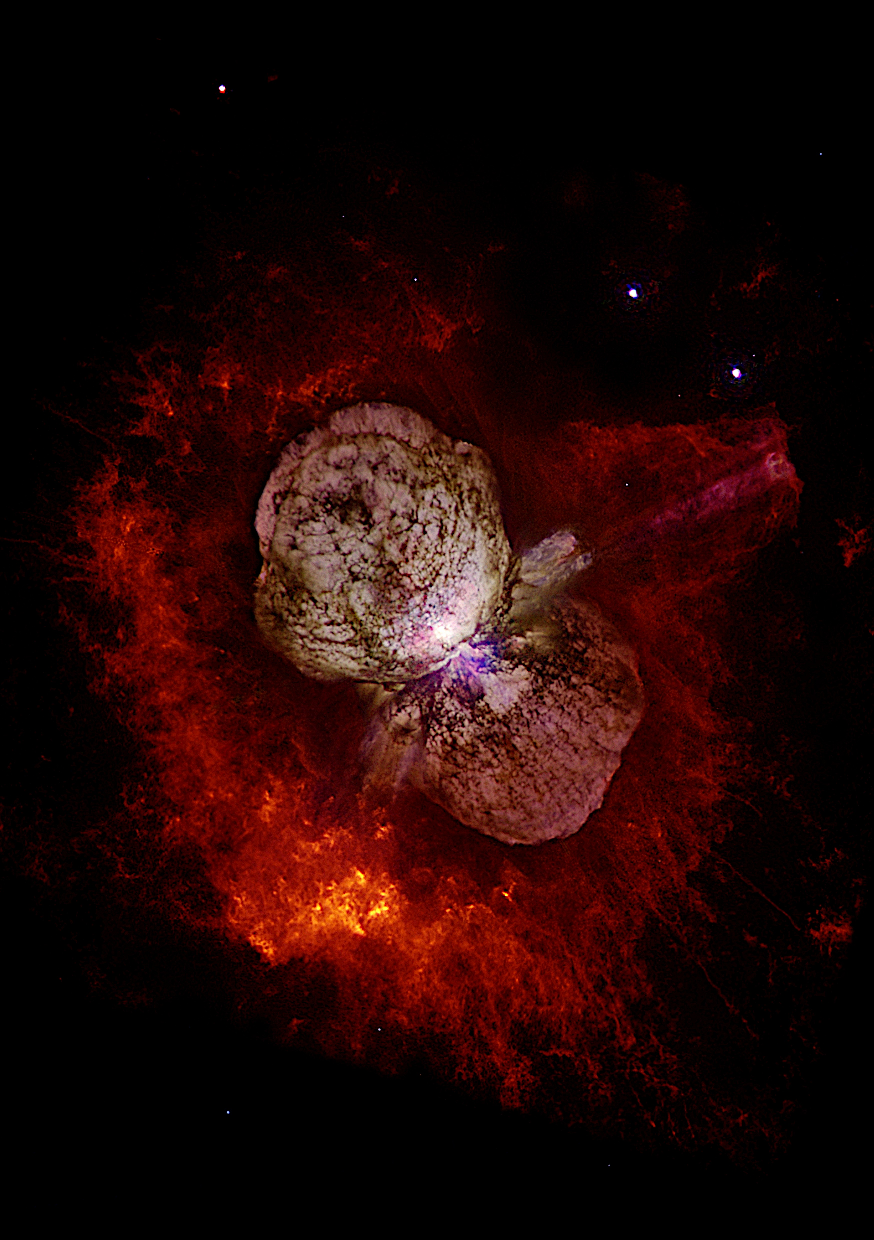
\includepdf[pages=-]{z-include-homunculus-a5.pdf}

Exakt einen Örzröt nach der vorherigen Meldung traf an dem Punkt, den das fünfte Lesezeichen im Navigationssystem beschrieb, die angekündigte Meldung ein.

\ialoudspeaker{»Dritte Sendung. Wechsel zum siebzehnten Briefkasten, falls ihr die Verfolgungspläne fallenlassen möchtet. Ansonsten Wechsel zu Eta Carinae ABC 2, ziemlich stabil dreihundertdreiundsechzig Lichtstunden vom Tripelstern entfernt. Es warten blühende Landschaften und postapokalyptische Metropolen auf euch. Bitte überlegt euch das noch mal gut, lasst euch nicht erwischen und wartet lieber am siebzehnten Kasten. Dann überleben wenigstens drei Viertel der Mannschaft. Wir dringen derweil in das Innere des Planeten vor. Da laufen noch Maschinen. Ende.«}

»Mir war bisher nicht einmal bekannt, dass Eta Carinae überhaupt über Planeten verfügt«, gestand Orakel.

»Den Äöüzz auch nicht«, zitierte yury die Datenbank. »Schon gar nicht im lebensfreundlichen Bereich. 363 Lichtstunden sind 1306800 Lichtsekunden, 2619 astronomische Einheiten. Orakel?«

Der Navigator war sofort mit weiteren Daten zur Stelle. »Eta Carinae besteht aus drei Sternen, die zusammen etwa fünf Millionen Mal so hell wie die Sonne strahlen. Die solare Leuchtkraft ist definiert als 3,828 mal zehn hoch 26 Watt.«

»Die brauchen wir tatsächlich gar nicht«, bemerkte yury. »Die fünf Millionen genügen: Die Quadratwurzel aus fünf Millionen 1,1-Teln ist 2132, das ist die innere Grenze der habitablen Zone in astronomischen Einheiten Distanz zum Zentralstern. Wenn man die Zahl unter dem Bruchstrich durch 0,53 ersetzt, kommt 3071 heraus. Die von Alexandra genannte Entfernung befindet sich also tatsächlich mitten in der Zone.«

Free runzelte die Stirn. »Ich habe gehört, die Helligkeit von Eta Carinae sei sehr variabel.«

»Das ist sie nach außen hin auch«, erklärte Orakel. »Besonders für die weit entfernten Menschen auf der Erde. Dort glaubt man auch bis heute, es handele sich nur um ein Doppelsternsystem. Die variable Helligkeit entsteht durch verschiedene Faktoren, von denen der Planet nicht betroffen sein muss. Der Homunkulusnebel beispielsweise verdeckt die Sicht. Es gab auch mal so etwas wie eine Supernova, aber das ist inzwischen auch knapp achttausend Jahre her. Die Äöüzz kennen Mittel und Wege, die Zivilisation vor Strahlenausbrüchen instabiler Sterne zu schützen, und wer auch immer die Metropole errichtet hat, wird ähnliche Schutzvorrichtungen gehabt haben.«

»Dass vor achttausend Jahren ein blühendes Sternenreich durch ›etwas wie eine Supernova‹ beendet wurde, hältst du für ausgeschlossen? Alexandra sprach von einer Postapokalypse.«

Das hielt Orakel in der Tat für ausgeschlossen. »Die Pseudo-Supernova war klar im Voraus berechenbar. Man musste die Sterne nur ein paar Tage beobachten, um festzustellen, was da wann passieren wird. Wie gesagt, selbst die Äöüzz können das. Wir haben es hingegen mit einem Volk zu tun, das zehn Lichtminuten durchmessende Felskugeln um seine Kraftwerke baut. Eine davon haben wir gefunden; die Äöüzz halten sie für die einzige Präsenz ihrer neuen Feinde.«

yury puzzelte die Informationen gedanklich zusammen. »Das würde erklären, dass es bisher keine Antworten auf unsere Funksprüche gab. Das Kraftwerk wird vollautomatisch von Robotern betrieben.«

»Und die betreiben vollautomatisch eine Kanonenbootpolitik mit uns?«, stichelte Free. »So richtig mit Racheakten und Warnzerstörungen unbewohnter Planeten?«

»Kann doch sein«, fand yury. »Unsere Bergbauroboter replizieren sich bereits selbst aus den gewonnenen Rohstoffen. Unser Quantencomputer hat eine Planetenregierung zu Fall gebracht. Warum sollten noch weiter entwickelte Roboter sich nicht genau so verhalten, wie sie es vor unserem Abflug noch getan haben?«

»Alexandras Beschreibung und der Sternenreich-Theorie nach würde das bedeuten, dass dort Roboter für Personen arbeiten, die inzwischen nicht mehr leben.«

»Das wäre extrem bitter.« Orakel schüttelte sich. »Dann wäre jede Maßnahme der Äöüzz gegen diese fehlgeschalteten Roboter ein lange überfälliger Schritt zum Schutz der Milchstraße. Gleichzeitig wäre jede verlorene Welt ein frustrierend sinnloses Opfer.«

»Für Roboter, die außer Kontrolle geraten sind.« yury und Free stimmten zu: Falls das der Fall war, musste der ethische Aspekt der Diplomatie neu bewertet werden. Andererseits: Wenn künstliche Siliziumverbünde solche Leistungen vollbrachten, wo war dann der Unterschied zu natürlich gewachsenen Silizium-Intelligenzwesen? Standen Robotern ab einem gewissen Intelligenzgrad möglicherweise Menschenrechte zu?

»Nennen wir es das Mechanische Reich«, schlug dessen Entdecker vor. »Selbst falls organische Wesen irgendwo die Zügel in der Hand halten.«

Damit waren alle einverstanden. »Gern«, sagte yury. »Dringen wir jetzt in das Mechanische Reich ein oder fliegen wir zum siebzehnten Briefkasten?«

Orakel hatte dazu eine klare Meinung. »Alexandra hat keine Wartezeit genannt. Das hat zwei Gründe: Erstens glaubt sie sowieso nicht daran, dass wir dort warten, und zweitens kann es sein, dass sie ohne unsere Hilfe bei dieser Mission umkommt. Wir können also gar nicht warten.«

Seine beiden Kollegen bezweifelten stark, dass man PHÖNIX helfen konnte; eher stand man den Agenten im Weg herum. Trotzdem führte kein Weg daran vorbei: Der Türbö Tächyön 1033 schoss mit hoher Beschleunigung gen Eta Carinae. Das Ziel war als galaktischer Leuchtturm und hellster Stern des Nebels schwer zu verfehlen.


\chapter{Ungeladene Partygäste}

Das Grauen der mechanischen Invasion gewann eine neue Dimension, als die ersten Krankentransporte über Hönüktün V angegriffen wurden. Die inzwischen für schnelle Evakuierungen gerüstete Sanitätstruppe traf einige Minuten zu früh über der frisch zerstörten Welt ein und wartete darauf, dass das Militär die letzten Angreifer in Antimaterieexplosionen aufgehen ließ. Überlebende in Rettungszentren des Planeten bereiteten sich darauf vor, von den weiß-roten Kugelschiffen aufgenommen und in sicherer Distanz auf vergleichbaren Planeten abgesetzt zu werden. Die stets unbewaffneten Rettungsflüge wurden von Funksignalen begleitet, die inzwischen auch den Invasoren als Äquivalent zum irdischen Rotkreuzsymbol bekannt sein mussten. Sie waren mehrfach in Situationen verschont worden, in denen Polizei- und Militärschiffe unter Laserbeschuss verglüht waren. Die Besatzung der Kugeln rechnete mit Streufeuer, nicht jedoch mit gezielten Angriffen.

In einer zweiten Welle aus der gegenüberliegenden Richtung traf Verstärkung ein, die es in dieser Form noch nicht gegeben hatte. Der kompakte Verbund aus Sanitätern war das erste Ziel, die planetaren Fluchtorte folgten unmittelbar darauf. Bevor das Militär einschreiten konnte, lebte über und unter der aufgeheizten Atmosphäre kein Zivilist mehr. Die Angreifer flohen nach vollbrachter Tat und fielen in das nächste System ein, wo sich gezielte Angriffe auf Bevölkerungszentren wiederholten. Die sinnlose Verbreitung maximalen Leids war entweder das Ergebnis einer Missverständniskorrektur oder einer neuen politischen Ausrichtung; man wusste nicht, ob die Roboter zuvor die Planeten für das wertvollste Gut der Äöüzz gehalten hatten.

Giämbättistä Vitällö saß ein wenig abseits, als Älföns Ögnöwäk eine Pressekonferenz gab. Er hatte die Verantwortung größtenteils aus der Hand gegeben und enthielt sich zunächst einer Stellungnahme.

»Uns fehlen die Worte, um das Gesehene mit ausreichendem Abscheu zu beschreiben. Uns fehlt eine Technologie, die zukünftige Angriffe im Voraus verhindert und uns aus der Beobachterrolle befreit. Haben wir einen Angriff zurückgedrängt, folgen zwei neue. Retten wir die Zivilbevölkerung, greift man diese gezielt an. Wir machen Fortschritte im Schlüssellochnebel, müssen uns jedoch den Vorwurf eines potenziell endlosen Stellungskriegs gefallen lassen. Wir führen zehrende Materialschlachten und sehnen uns nach Frieden, doch die Angreifer lehnen jede Kommunikation ab.«

Ein nie zuvor eingeladener Besucher erschien auf der Bühne. Diejenigen im Publikum, die nicht mit dieser Ankündigung gerechnet hatten, sahen überrascht zu Konrad Irby empor, der sich kurz verbeugte und neben dem Flottenadmiral Platz nahm. Der Besitzer des Germania-Systems, De-facto-Diktator der uggy-Piraten, wirkte ungewöhnlich betrübt, strahlte nur einen Bruchteil seiner üblichen Überheblichkeit aus und hatte den Kopf gesenkt.

»Verehrte Damen und Herren, Sie kennen mich bereits. Vermutlich hassen Sie mich; damit kann ich leben. Ich hatte die Produktion des Raumschiffs veranlasst, mit dem El Dörädö das Handwerk gelegt wurde, und ich hatte dessen Nutzung durch yury, Free und Alexandra freigegeben. Letztere hat übereifrig mein Büro in Flammen gesetzt, weil ihr von mir freigeschalteter Zugangsschlüssel nach einer etwas inkompetenten Manipulation durch Äöüzz-Ingenieure nicht mehr funktionierte. Ich betrachte den Vorgang mit Nachsicht als notwendiges Übel, um dem organisierten Verbrechen ein für alle Mal das Handwerk zu legen.«

Irby hob den Blick und fuhr fort:

»Nach der von mir etwas voreilig veranlassten Selbstzerstörung des Galaxievernichters verbleiben drei produktionsgleiche Raumschiffe, um deren Nutzung durch die Äöüzz ich heute bitten möchte. Ich brauche…«, er brachte es nur mit Überwindung über die Lippen, »kompetentes Fachpersonal für meine Technikwunder. Es wird Jahrhunderte dauern, bis wir gelernt haben, diese Schiffe so einzusetzen, wie sie jetzt benötigt werden.« Dann wies er auf eine Art Leinwand, an der zuvor ungesehene Schreckensbilder erschienen. »Wie Sie sehen, sind die uggys, unsere Patrouillen und unsere Planeten von dem Einmarsch der fnord~– Ihnen bekannt als das Antimaterie-Reich~– nicht verschont geblieben. Wir befürchten einen Angriff auf ugghy, dem wir nur offensiv zuvorkommen können, da gegen die Planetenzerstörungen kein wirksames Defensivmittel bekannt ist. In Zeiten externer Bedrohungen müssen wir am selben Strang ziehen und akzeptieren, dass es unterschiedliche Vorstellungen bei der Innenpolitik gibt. Wir haben sämtliche Polizeiaktionen gegen Mitglieder der Wirtschaftsvereinigung eingestellt.«

Im Hintergrund lief bereits die Besatzung der Raumschiffe. Es blieb auch nicht bei Herrn Irby: Zwei weitere Gruppierungen warben in Videobotschaften für ihren Anschluss an das Bündnis. Zunächst wurde die Flagge der Vereinten Nationen gezeigt, anschließend deren aktueller Generalsekretär.

\ialoudspeaker{»Die Bevölkerung des Sonnensystems bittet um die Gründung einer südgalaktischen Interessengemeinschaft, der wir ausschließlich zivil beitreten möchten. Wir verurteilen jede Form von Krieg, erkennen aber die generelle Notwendigkeit übergeordneter Verhandlungen über die Zukunft der Galaxis an.«}

Anschließend sprach ein Wesen in Kapuzenkutte, dessen Körperform auf dem Bild nicht erkennbar war, mit schattenverhülltem Gesicht und tiefer Stimme zu den Äöüzz.

\ialoudspeaker{»Der heilige Mrmbl-Orden fordert die sofortige Auslieferung der sieben Schwerverbrecher, die unseren Geheimplaneten ZX-25 Alpha 3 entweiht und durch Landungen beschmutzt haben. Anschließend sind wir nach Übergabe einer geeigneten Ablasszahlung dazu bereit, Gammaraumschiffe zur Verteidigung der Äöüzz-Wirtschaftsvereinigung und der uggy-Systeme bereitzustellen.«} Es folgte eine Dauerwerbesendung für die Mrmbl-Religion.

Das fand sogar Konrad Irby befremdlich. »Ich bitte darum, dieses verstörende Video zu unterbrechen.«

Vitällö nickte; das Bild verschwand. »Das Parlament hat den Vorschlägen aus Söl und Germania zugestimmt und eine Kooperation mit den Mrmbl abgelehnt. Für Ihre Fragen stehen wir nun zur Verfügung.«

\begin{center}
∞∞∞
\end{center}

Orakel, Free und yury ahnten nichts von der erneuten Eskalation in ihren Heimatsystemen. Mit zwei Billiarden Metern pro Sekunde, der sechseinhalbmillionenfachen Lichtgeschwindigkeit, brachte ein roter Blitz drei irdische Gestalten an einen Ort, der weit außerhalb der Wirtschaftsvereinigung und abseits des Kriegsgeschehens zum eigentlichen Hauptschauplatz werden sollte.

Vor dem Abschluss seines möglicherweise letzten Fluges verspürte yury ein dringendes Bedürfnis, die Bordtoilette aufzusuchen. Er übergab die Pilotenrolle an Orakel, ließ Free übergangsweise im Kapitänssitz die Stellung halten und verließ das Cockpit.

»Die Sessel in der 737 waren etwas bequemer«, fand Free. »Daran könnten die Äöüzz noch arbeiten.«

Orakel erklärte ihm, dass bei Sportschiffen wie dem Türbö Tächyön 1033 absichtlich auf manche Komforteigenschaften verzichtet wurde, da die Käufer dies üblicherweise so wünschten. »Das ist doch auch bei unseren Sportwagenfederungen seit jeher der Fall.«

Free lächelte. »Du wirkst nachdenklich.«

»Ich zerbreche mir seit einigen Minuten den Kopf darüber, ob es strategisch sinnvoll war, aus dem Zielbereich eines Funk-Richtstrahls an das darin genannte Ziel zu fliegen. Das schränkt unsere Anflugwinkel nämlich sehr stark ein.«

Seine Bedenken waren definitiv berechtigt. Eigentlich wollte er zwei Lichtminuten vor dem Ziel die Warpblase platzen lassen, doch diese Arbeit nahm man ihm kurz vorher ab.

»Blauinduktoren aktiv«, murmelte Free. »Schade, der Flug war bis gerade eigentlich sehr angenehm.« Dann verlor das Schiff seine Überlichtgeschwindigkeit. Einen zentralen Schiffsalarm gab es nicht; yury war ohnehin noch zu beschäftigt, um sinnvoll eingreifen zu können.

Um den Türbö Tächyön herum wurden tausende kleine Roboterschiffe sichtbar, die den Angreifern über Nögnög und Hönüktün ähnelten und eine ähnliche Zerstörungskraft entfalteten. Ohne Verhandlungsversuche, ohne Warnschüsse und von allen Seiten regneten weiße Laserstrahlbündel, tödliche Regenbogenkompositionen auf ungewöhnlich schlecht fokussierte Punkte herab, an denen sich wohl die Erdmenschen befinden sollten. Ein Teil der Strahlen schlug in die schwachen Schutzschilde des Rennschiffs ein und brachte diese irisierend zum Flackern.

Das Schiff rotierte um seine Achsen und geriet ins Trudeln, flog in einer groben Spirale durch den vorderen Teil der Angreiferkugel und riss zwei der Kügelchen mit sich, die glücklicherweise erst spät kollidierten und eine Kettenreaktion auslösten. Exponentiell anwachsend verabschiedete sich die Wolke der Wegelagerer, blies als blendend weißer Sternenwind die flackernden Schilde in Flugrichtung davon und verbrannte das Heck des Tächyöns. Es war, als hätte Orakel in seinem Pilotensitz einen Tritt gegen den Rücken erhalten, obwohl Andruckabsorber jeden solchen Einfluss schluckten.

Neu eintreffende Robotschiffe wurden durch einen ungesunden Beschleunigungsstoß mit den letzten Wasserstoffreserven abgehängt. Viel zu nah an der Lichtgeschwindigkeit und nur noch eine Minute vom Zielplaneten entfernt fehlte dem Türbö Tächyön ausreichender Treibstoff für eine Stabilisierung des Chaosflugs. Als das Schiff in die Atmosphäre einschlug, waren die Schutzschilde nur unzureichend aufgebaut und vergingen in der Reibungshitze. Eine Druckwelle, weithin angekündigt durch das Glühen eines Jahrtausendkometen, fraß den Impuls auf und verbreitete ihn über die Planetenoberfläche, wo er Fensterscheiben zerbersten ließ und die Pflanzenwelt einäscherte. Das gemeinschaftlich gekaufte Spaßschiff durchstieß auf einem Berg eine gläserne Sporthalle mit mehreren grünen Spielfeldern und Netztoren, versengte die weißen Strafraumlinien und durchstieß in vollem Umfang mehrere Tore. Außen am Gebäude zeugten zwei gegenüberliegende Wandschäden von Beginn und Ende des Spieleingriffs. Orakel klammerte sich an das effektlose Steuerruder, riss es an sich heran und konnte doch nicht verhindern, dass es weiter bergab ging. Hinter ihm krachte das Haus zusammen, vor ihm schlug die metallene Schiffsnase in einen Asphaltparkplatz ein, sodass das Gefährt mit einem 45-Grad-Winkel zur Gravitation bruchgelandet stecken blieb. Ein paar bitumengebundene Steinbrösel flogen umher.

»Und das alles ohne Airbags«, erzählte Orakel stolz dem aus der Toilette gestolperten Kommandanten.

»Kann man dich nicht einmal für fünf Minuten allein am Steuer lassen?«, stöhnte yury, bevor er zusammenbrach und für einige Minuten nicht ansprechbar war.

\begin{center}
∞∞∞
\end{center}

Rennschiffe waren üblicherweise nicht dafür konstruiert, \emph{in} einem Parkplatz abgestellt zu werden. Das auf seiner Längsachse unschön gestauchte, kollisionsverbeulte Metallstück hatte trotz roter Kriegsbemalung wenig Chancen, in einem Gebrauchtwagenkatalog außerhalb der Schrottabteilung gelistet zu werden. Schleusen hatte es sicherlich einmal gegeben; derzeit wirkten die verbeulten Aussparungen, als habe jemand den Begriff »abgerundetes Rechteck« mehrdimensional interpretiert. Als Ausgang ungeeignet und durch schlechte Planung alternativlos banden sie die drei Bruchpiloten an das Innere ihres Ex-Sternengefährts.

»Top«, sprach Alexandra zu sich selbst. »Meine Kollegen bieten mir stets die Unterstützung, die ich in meinem Job brauche.«

Ob sie damit den mittelschweren Plutonium-Dreieckslaser oder die Insassen des Türbö Tächyön meinte, war unklar und unwichtig. Letztere wurden durch Ersteren befreit, was sich von außen als machbare Fleißarbeit erwies, von innen hingegen durch Überhitzung zum Scheitern verurteilt gewesen wäre. Durch die großzügig bemessene Frontscheibe, mit Videobrillen auf den Augen, verfolgten yury, Orakel und Free gespannt ihre eigene Bergung.

»Das nennt man wohl moralischen Beistand«, spottete sie; das letzte Halterungsstück trat sie mit dicken Stiefeln nach innen. »Herzlich willkommen auf Eta Carinae ABC 2. Ihr könnt die Helme abnehmen, die Luft ist atembar. Eure Ankunft war übrigens kaum zu überhören. Saß Free am Steuer?«

Orakel grinste. »Schon, ein bisschen. Genug, um uns aus einer Kugel aus Feuerkugeln zu befreien.«

»Natürlich ist Orakel geflogen«, verriet ihn yury. »Ich hatte mir nur kurz die Hände gewaschen und auf einmal gab es einen lauten Knall.«

Orakel störte das nicht im Geringsten. Er zog eine Dose Macadamianüsse hervor und stärkte sich unter den abwartenden Blicken seiner Freunde für die kommende Mission. Eine große Portion Frischwasser und zweihundert Gramm ungewürztes Popcorn rundeten das Mahl ab, dann verließ die Gruppe geschlossen das Raumschiff. Draußen wehte ein sanfter Bergwind bei etwa 360 Örztemp, die in den Raumanzügen auch ohne hermetische Abriegelung gut erträglich waren. Der demolierte Parkplatz befand sich an einer Klippe; etwa siebenhundert Meter tiefer erstreckten sich Pflanzen in Stadtform über eine große Fläche, unterbrochen von wurzeldurchdrungenen Straßenresten in tristem Quadratlayout. Ein paar Häuser überragten den Rest; sie waren nur bis zu einer gewissen Höhe von efeuähnlichen Pflanzen überwuchert. Aus der Ferne sah alles aus wie ein grüner Sumpf, aus dem an einigen Stellen Metall, Glas und Beton ragten.

»Und was machst du hier?«, fragte Free verwundert. Dann streckte er ihr herausfordernd die Zunge entgegen. »Außer uns mal wieder aus einer Lage zu befreien, in die wir ohne dich nie geraten wären.«

Alexandra lachte durch die Nase und rollte mit den Augen. »Erzähl das Orakel. Siehst du die vier Hochhäuser da unten?«

Vier identisch aussehende Wolkenkratzer waren auf zwei Dritteln ihrer Höhe mit Bogenbrücken verbunden~– Free zog die Brille wieder auf~– geländerlos aus purem Glas. »Das ist jetzt wohl modern, ja?« Die Diagonalbrücke hatte die Form eines Kreuzes und überragte die Seitenbrücken. Vielleicht war das Material oberseitig aufgeraut oder in irgendeiner Form gestuft, sonst handelte es sich um ein sehr rutschiges Beförderungsangebot.

»Ich vermute, dass dieser Gebäudekomplex eine zentrale Bedeutung für das Antimaterie-Reich hat.«

»Mechanisches Reich«, sagte yury. »Wir haben es umbenannt. Vielleicht treffen wir irgendwo noch auf einen organischen Repräsentanten dieses Wahnsinns, aber ich glaube nicht mehr daran. Niemand von uns tut das.«

»Einverstanden«, bekundete Alexandra und erklärte weiter: »P, H, Ö, N und I befinden sich jenseits des Horizonts in einem selbst geschaffenen Tunnel. Wir haben unterirdische, künstlich wirkende Hohlräume detektiert und wollten dorthin vordringen, um einige Geheimnisse zu lüften. Mein Smartphone hat mir bei der Landung gemeldet, dass ihr mir folgen würdet, auch wenn ich nicht verstehe, wie ihr das fertiggebracht habt. Ich dachte, wir hätten alle Spuren verwischt und recht ungewöhnliche Ziele gewählt. Und dass Eta Carinae einen erdähnlichen Planeten beherbergt, konntet ihr unmöglich wissen.«

»Aber du hast doch Koordinaten für tote Briefkästen in den Türbö Tächyön eingespeichert, als du auf der Erde warst«, wollte Free sie erinnern. »Und du hast uns Funksprüche–«

»Ich war lange nicht mehr auf der Erde. Funksprüche? Was?« Alexandra wurde hellhörig. »Der Goldtransport war mein letzter Erdaufenthalt. Und ich kann dir garantieren, dass niemand von uns Funksprüche gesendet hat: Wir haben strikte Funkstille gehalten und uns über Kabel unterhalten, bis wir gemerkt haben, dass wir auf dieser Welt vor dem Zugriff der Roboterschiffe sicher sind. Die meiden diesen Planeten wie eine große Tabuzone. Das spricht übrigens ebenfalls dafür, dass wir am Ziel angekommen sind.«

»Im Türbö Tächyön auf der Erde war jemand, der dort Erdspuren auf dem Boden und Koordinaten im Bordcomputer hinterlassen hat. Die Koordinaten waren mit Notizen versehen, die dich als Absenderin ausgeben. Wir sind dorthingeflogen und haben dort Funksprüche empfangen, die in deiner Stimme von eurem Fortschritt berichteten.«

»Das ist unmöglich«, behauptete Alexandra.

Free verzog das Gesicht. »Wie du siehst, hat irgendjemand das möglich gemacht. Gruselig.«

»Können wir uns jetzt bitte auf die Mission konzentrieren?«, bat Orakel. »Da unten warten vier Hochhäuser auf ihre Erkundung. Etwa zwei Lichtminuten über uns schweben sicherlich noch ein paar tödliche Kugeln voller Antimaterie, die derzeit aus unerfindlichen Gründen nicht über uns herfallen. Im Inneren der Häuser würde ich mich zumindest weniger beobachtet fühlen.«

»Und die Kantine plündern«, sagte yury voraus. »Bis auf die Funkstille klingt das alles einigermaßen plausibel. Dann mal los.« Er sprang mit aktiviertem Jetpack voran und ließ sich sanft in die Tiefe tragen.

\begin{center}
∞∞∞
\end{center}

Als die vier Menschen im Dschungel unter der Häusergruppe angekommen waren, wurden ihnen die Höhe und die Größe der Türme erst richtig bewusst. Vielleicht befand sich unter dem Efeu ein Markenlogo, irgendein Schriftzug, zumindest Hausnummern, doch alles war grün bedeckt. Einen Haupteingang gab es allerdings; dieser wurde von Pflanzen dauerhaft offen gehalten und hatte wohl früher eine automatisch öffnende Schiebe-Glastür mit Bewegungsmelder dargestellt. Die farnlastige Flora zog sich bis weit ins Innere des Erdgeschosses. Ehrfürchtig betraten die vier Besucher das Gebäude.

»Vielleicht hat man an der Rezeption Informationen für uns«, hoffte Alexandra.

»Bekommst du von PHÖNIX eine Nachricht, wenn sie etwas finden?«, erkundigte sich Free.

»Selbstverständlich«, bestätigte Alexandra. »Die Kolleginnen wissen über unsere Aktion ebenfalls Bescheid. Sie glauben aber nicht wirklich, dass wir hier etwas finden.« Mit der Befürchtung, eine allzu rabiate Beschädigung der Efeustränge würde den Zorn der ganzen Pflanzenwelt auf sie ziehen, schob das X von PHÖNIX einige Laubblätter vom Empfangstresen. Es kamen tatsächlich bedruckte Folien zum Vorschein, hauptsächlich in Telefonbüchern und Kalendern, witterungsfest und künstlich, wie es sich für eine moderne Zivilisation gehörte.

yury stand neben Alexandra am Tresen und untersuchte das Material. »In den Funksprüchen wurde uns gesagt, ihr habet Überreste einer raumfahrenden Gruppierung gefunden, die fast spurlos von ihren Planeten verschwunden sei. Ist das richtig?«

Erneut war Alexandra über die Detailtiefe der Funknachrichten überrascht. »Das ist zwar richtig, aber das haben wir nie gesendet. Kann ich mir Aufzeichnungen von dem anhören, was da in meinem Namen gesendet wurde?«

»Natürlich.« yury blickte zu Orakel hinüber, der scheinbar gedankenverloren eine angeschimmelte Wand musterte. Aus den Außenlautsprechern dessen Raumanzugs ertönte die Stimme einer Person, die plötzlich begriff, auf welcher Basis die Nachrichten generiert worden waren.

»Meine Audio-Tagebucheinträge«, rief Alexandra. »Mit künstlich erzeugter Funkverpackung am Anfang und am Ende. Von ›Briefkästen‹ habe ich nie geredet, und ich beende meine Tagebucheinträge einfach durch Abschalten der Aufzeichnung.« Sie hörte sich die restlichen Nachrichten noch geduldig an, dann echauffierte sie sich lautstark über die mit diversen Kraftausdrücken belegte Person, die es gewagt hatte, ihr Tagebuch in Auszügen durch die Galaxis zu schicken. Da vorerst mangels Personenkenntnis keine Möglichkeit bestand, die impulsiv angedrohten Racheakte in die Tat umzusetzen, stöberte sie murrend weiter in den Folien herum. »Das ist ein Verwaltungsgebäude«, schloss sie dann. »So etwas wie das Rathaus in Toronto.«

»Kannst du die Sprache lesen?«, fragte yury erstaunt.

»Behördenpapiere sehen auf jedem Planeten gleich langweilig aus, haben stets die gleiche Absatzform und kommen in dieser Häufung nur bei notorischen Stammkunden und Gastgebern vor.« Sie hielt zwei Exemplare in die Höhe und jeder wusste, was gemeint war.

»Gewagt, aber nicht absurd«, fand Free. »Findet ihr auch, das sieht irdischen Hieroglyphen noch am Ähnlichsten?«

»Das Alphabet, wenn es eines ist, wirkt tatsächlich ziemlich bildhaft«, bestätigte Alexandra. »Das da könnte ein Vögelchen sein. Eine kleine Meise.«

»Das da sieht aus wie ein Hamburger«, meldete sich Orakel zu Wort. »Mit zwei Buletten.«

yury schüttelte den Kopf. »Es könnten auch Eisenbahnschienen sein. Es kann eigentlich \emph{alles} bedeuten. Dass hier überhaupt Hochhäuser stehen, wie wir sie kennen, ist bereits beachtenswert. Nicht jede raumfahrende Intelligenzform baut quaderförmige Glaskisten, um ihre überzähligen Bewohner möglichst billig auf kleiner Fläche unterzubringen.«

Das fand Orakel nicht ganz schlüssig. »Die Menschen tun das, die uggys auch, die Äöüzz bevorzugen planetare Expansion, tun es aber trotzdem. Ist das wirklich so überraschend?«

»Die Ameisenwesen aus dem Dönkwön-System wären ein Gegenbeispiel. Die Käfer von Frzn finden rechte Winkel und Glasscheiben ebenfalls nicht besonders toll. Wenn man schon eine Behausung baut und sich dorthin zurückzieht, will man aus deren Sicht doch gar nicht nach draußen gucken.«

»Das heißt also«, wollte Orakel mit einer Antwort beginnen, doch yury bat noch kurz um eine Fortsetzung:

»Es wäre kurzsichtig, jetzt nach den entscheidenden Gemeinsamkeiten und Unterschieden zu suchen, um daraus eine Regel abzuleiten. Man verrent sich da sehr schnell in Fehldefinitionen, weil die Stichprobe sehr, sehr klein ist. Wenn wir tausende raumfahrende Gruppen betrachten könnten, gäbe es stochastische Möglichkeiten zur Analyse. So gibt es hingegen nur unqualifiziertes Raten. Auch mit der Bewertung der bedruckten Folien sollten wir vorsichtiger sein.«

Free zeigte auf eine Kameralinse seines Anzugs. »Was die fremden Sätze und Schriftzeichen angeht, können wir durchaus tausende Exemplare sammeln und untersuchen lassen. Wir fotografieren einfach alles ab, was wir finden.«

»Ich befürchte, wenn wir die Ergebnisse in den Händen halten, ist es zu spät für eine Entschuldigung«, mutmaßte yury. »Die Äöüzz benehmen sich wie Elefanten im Porzellanladen, und wir nehmen vielleicht gerade das Allerheiligste auseinander. Wir sind keine Archäologen, spielen uns aber wie welche auf.«

»Sollen wir Experten vom Kommunikationsinstitut hinzurufen?«, spottete Alexandra. »Wenn die nur halb so freundlich empfangen werden wie ihr, kommen sie nie hier an.« Die ganze Ethikdebatte vernachlässigte die reale Bedrohung aller bewohnten Systeme der Südgalaxis. Es bestand akuter Handlungsbedarf, und Alexandra ging ohne weitere Diskussion auf eine stählerne Doppeltür zu, die nach einem Aufzugzugang aussah. Der Knopf daneben trug das zuvor angesprochene Meisensymbol, das vielleicht für ›oben‹ oder ›himmelwärts‹ stand. Dass dessen Beleuchtung auch nach einem Knopfdruck dunkel blieb, war eigentlich selbstverständlich. In dieser Stadt führten die Leitungen keinen Strom mehr.

Nach zwei Minuten Wartezeit erklärte die Gruppe den Aufzug endgültig für unbrauchbar und entschloss sich dazu, es über das Treppenhaus zu versuchen. Die automatische Schiebetür dazu war ebenfalls verschlossen, aber wenigstens aus zerbrechlichem Material.

»Einscheiben-Sicherheitsglas«, kommentierte Orakel die Bruchstücke auf dem Treppenhausboden. »Absichtlich dauerhaft unter Druck- und Zugspannungen stehend, damit es bei Beschädigung sofort komplett in kleine Einzelteile zerfällt.«

»Praktisch« fand Alexandra das. Sie befand sich bereits fünf Stufen weiter oben und blickte den Schacht empor. »Leider kommt man mit Jetpacks nicht durch die Mitte.«

»Wir können auch außen herum fliegen«, schlug yury vor. »Uns fehlt nur ein Ziel dafür.«

Orakel ging abwägend nach oben. »Ein paar Etagen sollten wir uns ansehen, bevor wir die ersten überspringen.« yury und Free schlossen sich an.

\begin{center}
∞∞∞
\end{center}

Oberhalb der zerbrochenen Glastür gab es offenbar keine Zugangssperren mehr. Der Treppenhausausgang und alle Räume der ersten Etage waren elektronisch durch Glastüren verschließbar, aber keine davon war geschlossen.

»Guckt mal, wie grün der Flur leuchtet«, rief Alexandra. »Das Sternenlicht scheint durch das Efeu.«

Orakel bewunderte die Blattstrukturen auf dem weißen Linoleumboden. »Das ist wirklich ein hübscher Effekt.«

yury fand die Farbe ebenfalls schön, schritt jedoch an den beiden Kunstkritikern vorbei in den nächstbesten Besprechungsraum und öffnete ein mannshohes Fenster. Die daran klebenden Pflanzen wurden nach innen gezogen, lösten sich mit einem Schmatzen von der Fensterumgebung und schreckten einige Krabbeltiere auf, die sich darunter eingenistet hatten. Free griff im Vorbeigehen nach einer Schere in Orakels Außentaschen und schnitt den Rahmen frei. yury ließ ihm den Vortritt; abwechselnd blickten sie sich nach draußen um.

Free winkte Orakel und Alexandra einladend zu. »Ich kann schon verstehen, warum die Brücken geländerlos und aus Glas konstruiert wurden. Das ist wohl eher als Zierde gedacht und sieht dabei ebenfalls sehr beeindruckend aus.«

»Habt ihr das Fenster nur für den schönen Ausblick freigelegt? Und das im ersten Obergeschoss.« Orakel stimmte allerdings zu, dass die Brücken schön gestaltet waren.

»Ich glaube, wir wollten vor allem überprüfen, ob wir im Notfall durch die Fenster nach draußen kommen.« Free zuckte mit den Schultern. »Und wie dicht die Botanik mit der Außenwand verwachsen ist.«

»Das da muss Eta Carinae A sein, der große Riese, der durch die ganze Galaxis strahlt.«

yury und Free befreiten ein weiteres Fenster direkt neben Orakel, um bequem gleichzeitig hinausblicken zu können. Der Stern stand hinter dem schräg gegenüberliegenden Hochhaus und schien durch alle Pflanzen und Fenster hindurch blauweiß. Die anderen beiden Sterne waren nicht erkennbar; dies würde sich auch in den nächsten Örzbits nicht ändern.

Die einzige Person, die nie die eigentliche Mission aus den Augen verlor, war offenbar Alexandra. »Ein Foliendrucker«, rief sie aus dem Nebenraum. Orakel und yury verschlossen die beiden Fenster wieder und liefen ihren Kollegen hinterher.

»Ein Serverschrank«, freute sich Free. Dann verzog er das Gesicht. »Ohne Strom.« Er zog ein schwarzes Stromkabel heraus, das irdischen Kaltgerätekabeln inklusive des C13-Steckers ähnelte. Genervt starrte er yury an.

»Na ja, das ist halt international standardisiert.«

»Sehr lustig. Was wird hier gespielt?«

yury zuckte in seltener Wissenslosigkeit mit den Schultern. »Wir sind hier, um das herauszufinden, würde ich sagen. Und ein Dreiphasen-Stromsystem mit rechteckigem Stecker und Einkerbungen zur Verpolungssicherheit ist jetzt auch nicht so unglaublich ungewöhnlich.«

Damit gab sich Free nicht zufrieden: Er verfolgte das Kabel durch einen Kabelschacht und zog das andere Ende aus seiner Steckdose. »Wenn das jetzt ein Schukostecker gewesen wäre, hätte ich das Handtuch geschmissen.«

»Was ist es stattdessen?«, erkundigte sich Alexandra.

»Irgendetwas Außerirdisches. Aber es hat drei Stifte und ist genauso verpolungssicher wie die andere Seite.«

»Das hat man in Deutschland bis heute nicht geschafft«, stichelte yury.

»Ich habe gehört«, erwiderte Free, »wenn man einmal im Dunkeln auf einen britischen Stecker getreten ist, wünscht man sich ein weniger hinterhältiges Steckersystem. Das wurde hier ziemlich elegant umgangen.«

»So sehen doch Starkstromstecker für Elektroautos aus«, meinte Orakel. »Also so ähnlich.«

Seine Freunde fanden, mit etwas Fantasie konnte man sich auf diesen Vergleich einlassen. Der Stecker hatte einen Außenring aus Plastik, drei Außennaben im Abstand von 90 und 180 Grad, an jeder Außennabe einen runden Leiter und durchmaß etwa vier Zentimeter.

»Gibt es hier Tastaturen?«, fragte Alexandra neugierig.

»Uns fehlt leider der Strom–«, entgegnete Free mit dem Kopf im Serverschrank.

Sie lachte und unterbrach ihn. »Ich würde aus den Tasten gerne Rückschlüsse auf das Alphabet ziehen, oder zumindest nachträglich ziehen lassen.«

Leider befand sich keine Tastatur im Schrank, keine bedruckte Folie in Druckernähe. Das Interessanteste, das der Raum noch zu bieten hatte, war der zu Staub gewordene Überrest von Erde in einem Blumentopf. Einen Raum weiter wurde Alexandra fündig.

Orakel lachte als Erster, als er die Glasplatte in Alexandras Händen sah. Zögerlich stiegen yury und Free mit ein. Alexandra schmunzelte und legte den Touchscreen zurück an seinen Platz. »Nicht einmal Fingerabdrücke sind darauf zu erkennen, nur noch Staub.« Sie pustete über den Schreibtisch und wirbelte Wolken aus grüngrauem Belag durch die gefilterten Sonnenstrahlen. Da die Geräte keine Beschriftung aufwiesen und selbst Markennamen fehlten, zog die Gruppe weiter zum nächsten Raum. Dieser war ein identisch eingerichtetes Büro, genau wie alle weiteren Räume bis auf die Toiletten.

»Selten sah man sprachlichen Sexismus in so deutlicher Form, dass ihn selbst Außerirdische verstehen«, beschwerte sich yury. Auf einer der beiden Türen befand sich das Meisensymbol, auf der anderen ein Unterstrich.

»Meinst du nicht, du interpretierst da möglicherweise zu viel hinein?«, fragte Orakel vorsichtig.

»Was soll es denn heißen außer ›oben‹ und ›unten‹? Das stellt doch eindeutig eine Hierarchie dar!«

»Na ja«, meinte Orakel und stieß die Meisentür auf. Dahinter befand sich eine Treppe nach oben. Er öffnete die zweite Tür; hier gab es nur ein großes Waschbecken zu sehen. Die beiden Räume waren durch eine Tür untereinander verbunden. »Vielleicht heißt es auch wirklich nur das.«

»Fließendes Wasser wird es jedenfalls kaum geben«, lenkte Alexandra den Blick auf das Wesentliche. Sie drehte einen der Wasserhähne auf, in denen sich vermutlich seit Jahrhunderten, möglicherweise Jahrtausenden kein Wasser mehr befand. Es strömte auch keines nach.

Ihre Freunde konnten gut verstehen, was sie gemeint hatte, als sie die Stadt als »postapokalyptisch« bezeichnet hatte. Alle möglichen Grauenvorstellungen, jedes Abschiedsszenario für eine Planetenzivilisation war längst Teil der unerreichbaren Geschichte geworden. Hier gab es nur noch die Natur und die wenigen Materialien, die von ihr nicht verwertet werden konnten. Wasser gehörte nicht dazu.

Orakel stieg die Treppenstufen hoch und drückte einige Kabinentüren zur Seite. »Es wird aber Regenfälle geben, Unwetter und Stürme. Ein paar kleine Tiere haben wir gesehen, vielleicht gibt es so etwas wie Bienen.«

»Gibt es da oben irgendwelche Überraschungen zu sehen?«, wollte yury wissen.

»Nee, das kennt man aus jedem öffentlichen Gebäude. Es sieht auf der Erde und auf Örz nicht anders aus. Hier haben Wesen gearbeitet, die zumindest in dieser Hinsicht einen ähnlichen Körperbau haben wie wir.«

Damit war die Untersuchung der ersten Etage abgeschlossen. Durch das Treppenhaus wurde die zweite Etage betreten, kurz durchstöbert, für gleich befunden und wieder verlassen. Die Handlungsschritte wurden fünf Mal wiederholt, dann beriet sich die Gruppe an zwei weiteren freigeschnittenen Fenstern mit Blick auf den höher gewanderten Stern.

yury grübelte. »Deine Kollegen von PHÖNIX haben dich allein losgeschickt, weil sie nicht glauben, hier etwas Wertvolles zu finden, richtig?«

Alexandra nickte leicht zerknirscht.

»Unser Problem ist wohl, dass wir in jeder übersprungenen Etage irgendetwas übersehen könnten. Hast du eine genauere Vorstellung davon, wonach wir eigentlich suchen?«

»Vorrangig nach Sprachdaten. In dieser Hinsicht war der Serverschrank im ersten Obergeschoss eigentlich bereits der Goldfund. Ich befürchte aber, da gibt es einen Haken.« Sie blickte Free an.

Free nickte. »Wenn wir irgendwo optische Datenträger finden, lässt sich vielleicht etwas machen. Alles andere hat nach dieser Zeit seine Magnetisierung oder seine Ladung verloren.«

»Für CDs ist diese Zivilisation zu modern«, fand yury. »Da werden wir eher in einem Museum oder in einer Bibliothek fündig. So etwas muss es in dieser Stadt doch auch geben.«

Das sah Alexandra ebenfalls so. »Irgendwo unten in der Stadt wird es eine Art ›Stein von Rosetta‹ geben, der uns die Sprache entschlüsselt.«

»Warum hast du dich dann für dieses Hochhaus entschieden?«, fragte Free verständnislos.

»PHÖNIX geht davon aus, dass es auf diesem Planeten etwas gibt, das die Verbohrtheit der Roboter beenden kann. So etwas wie eine große Fernbedienung. Da noch irgendwelche Maschinen im Planeteninneren laufen und Wärme erzeugen, sehen sich fünf Leute dort um. Dass eine Fernbedienung schon allein symbolisch nicht unter, sondern über die Erde gehört, und dass das größte Hochhaus der größten Stadt vielleicht die nötigen Informationen enthält, glaubt man mir eben nicht.«

»Selbst falls es hier die gesuchten Informationen gibt, könnten wir sie momentan nicht lesen«, erinnerte Orakel sie. »Vielleicht wäre ein Abstecher zum Museum doch ganz hilfreich.«

Alexandra wandte ein, noch wisse man nicht, ob eine solche Institution auf dem Planeten überhaupt existiere, aber eine kurze Suche könne tatsächlich nicht schaden. »Ein Museum als solches von außen zu erkennen, würde ich mir sogar hier zutrauen.«

Tatsächlich gab es einige Umrisse im Dschungel, die breiter waren als andere und von größeren Bäumen umgeben waren. Vielleicht hatte es sich um Villen mit großem Garten gehandelt, vielleicht um Museen mit großen Besucherparkplätzen.

yury, Alexandra, Orakel und Free verkeilten die Fenster, indem sie einen Schreibtisch freiräumten, zwei Bürostühle an die Scheibe schoben und diese mit dem Tisch am Fortrollen hinderten. Anschließend verließen sie das Gebäude durch die beiden Fenster und hofften, dass in ihrer Abwesenheit nicht alles wieder mit Efeu zuwucherte.

\begin{center}
∞∞∞
\end{center}

Das erste vermeintliche Museum war ein tristes Privatgebäude. Orakel fotografierte ein Kochbuch ab, den einzigen nichtflüchtigen Informationsspeicher des Hauses. Leider fand sich nicht unmittelbar eine Bestätigung für die Hamburger-Theorie; das Hamburgersymbol kam in allen Texten ungefähr gleich häufig vor.

Das zweite vermeintliche Museum war eine Sporthalle. yurys Vermutung zur Geschlechtertrennung wurde dadurch ad absurdum geführt, dass es nur eine einzige Umkleide gab. Ausflüchte, vielleicht handele es sich um eine Sporthalle nur für eine Hälfte der Bevölkerung, wurden als »nun wirklich an den Haaren herbeigezogen« abgetan. Dafür wusste man jetzt, dass die Planetenbewohner Kleidung getragen hatten. Man fand sogar die eine oder andere Polyestersocke, die in einer Ecke unter der Bank gelandet war. Vieles sprach für eine sehr erdähnliche Bewohnerschaft.

Das dritte vermeintliche Museum war zumindest eine Bibliothek. Dieser mangelte es jedoch an historischen Originaldokumenten; alles war auf Folien gedruckt und in Hartplastik gebunden. Fleißig digitalisierten die vier Erkunder den Sprachschatz.

Es waren schließlich die Daten aus dem Kochbuch, die bei der Klärung der letzten Fragen halfen. Die eingebauten Übersetzungscomputer der Raumanzüge waren leistungsfähig genug, um das Alphabet als solches zu erkennen und die zugrunde liegende Sprache grob zu erlernen.

\ialoudspeaker{»Bitte verlasse mich nicht«}, sprach Alexandras Computer, \ialoudspeaker{»es ist so dunkel dort draußen.«}

\ialoudspeaker{»Ich muss gehen«}, antwortete der Computer sich selbst in einer tieferen Stimme.

\ialoudspeaker{»Dann«}~– das war wohl der Erzähler~– \ialoudspeaker{»verließ Wolfgang das Haus.«}

Orakel packte das Buch und schleuderte es durch den Lesesaal, dann war er mit sich und der Welt zufrieden.

\begin{center}
∞∞∞
\end{center}

Zurück im Hochhaus nahmen Alexandra und yury den Dokumentenstapel von der Rezeption an sich und trugen diesen in die fünfte Etage. Orakel und Free kopierten das gesammelte Bildmaterial auf den Örztöp und sichteten die Sammlung.

»Für eine wirklich detaillierte Analyse fehlen uns der Quantencomputer und die Silizium-Rechenleistung der 4-6692«, berichtete Orakel. »Wir können aber erst einmal bestätigen, dass wir uns in einem Verwaltungsgebäude befinden. Die Bescheide, die Alexandra unten gefunden hat, sind für Verkehrssünder gedacht, denen die Fahrerlaubnis entzogen wurde. Wir schließen daraus: Hier gab es manuellen Individualverkehr äußerst freiheitsliebender, rebellischer Wesen, die längst über die Technik für autonomes Fahren verfügt haben müssen.«

»Vielleicht gab es auch einfach nur ganz viele dumme Autofahrer«, fand Free.

»Nicht alles, was man nicht selbst versteht, ist dumm«, widersprach Orakel. »Vive la liberté!«

yury lachte. »Das ist doch absurd.« Er griff nach einer der Folien. »Und die Meise bedeutet weder ›oben‹ noch ›unten‹, sondern einfach ›Eins‹. Der Unterstrich ist eine Null.«

»Vielleicht werden dieselben Zeichen auch für andere Begriffe als Abkürzung verwendet.« Alexandra überflog die Übersetzung und verglich diese mit dem Originaldokument. »Das Adressschema könnte aus Legisla stammen.«

»Damit sind wir ein riesiges Stück weitergekommen«, freute sich Orakel. »Möchtest du vielleicht deine Kolleginnen per Funk informieren?«

Gegen diese Kommunikationsmethode gab es große Vorbehalte, besonders von Alexandra selbst. »Über diese Distanz würde man das vermutlich bis ins Weltall bemerken. Ich glaube immer noch, dass die Roboter dazu in der Lage sind, auch die Inhalte der Nachrichten zu entschlüsseln.«

»Du meinst, falls wir hier zu viel herausfinden, schreitet man doch noch als Notfallmaßnahme ein?«

»Ja, das ist zu befürchten. Das schwebt ständig als Damoklesschwert über uns.«

»Eine andere Theorie wäre, dass die Roboter uns dankbar für diese Arbeit sind, weil sie diese nicht selbst vornehmen können.« Free trat an das linke Fenster und blickte zum Himmel empor. »Auch in diesem Fall wäre es aber gefährlich, seine Aufgabe abgeschlossen zu haben.«

»Wir sollten es zumindest nicht laut herausposaunen«, fand auch yury. »Wo genau sich deine Kolleginnen gerade befinden, wissen wir ja auch nicht. Vielleicht haben sie viele Kilometer im Planeteninneren zurückgelegt und schreiten schnell voran. Es kann sein, dass wir sie selbst dann nicht einholen würden, wenn wir es mit Jetpacks versuchten.«

»Also behalten wir unseren Fund für uns und suchen weiter nach einer Fernbedienung«, seufzte Orakel. »Es sind ja nur noch hundert Etagen übrig, die man durchstöbern kann.«

Alexandra versuchte, ihn aufzumuntern. »Ein paar davon kann man bestimmt überspringen. Und es sind nur achtundneunzig Etagen über uns, nicht hundert.«

Orakel, der die Zahl nur grob überschlagen hatte, war von der Bestätigung gar nicht begeistert. »Achtundneunzig Etagen! Uiuiui, ojeojeoje.«

Mit dem Ausspruch »Dann sind wir ja locker bis heute Abend fertig, los gehts« verließ yury den Raum und betrat das Treppenhaus. Es war nicht ganz klar, ob er eine Art Galgenhumor oder echte Hoffnung entwickelt hatte.

»Wir könnten wenigstens den Aufzugschacht aufschneiden, um uns schnell zwischen den Etagen zu bewegen«, schlug Orakel vor.

»Und dann auf jeder Etage von innen mit dem Laser arbeiten?«, hielt ihm yury die Schwäche seines Plans vor. »Da ist es effizienter, von außen immer die Scheiben kaputtzumachen. Oder mit den Jetpacks die Treppen hochzufliegen.«

»Dabei stößt sich jemand gehörig den Kopf, ich sehe das schon kommen«, prophezeite Alexandra. »Falls es euch nicht zu viel ausmacht, gehen wir ganz normal zu Fuß. Es gibt Leute, die rennen freiwillig das Empire State Building hoch, das ist genauso groß.«

»Das Empire State Building ist eine Etage kleiner«, spaltete yury sofort das ihm angebotene Haar, »und daher als Vergleich total ungeeignet.« Dann lief er grinsend die Treppe nach oben, hauptsächlich vor Alexandra davon, die ihm nun die Leviten lesen wollte. Orakel und Free packten schnell ihre Sachen zusammen und rannten mangels Alternativplan amüsiert hinterher.

\begin{center}
∞∞∞
\end{center}

Keuchend kam yury an einer Bürowand zum Stillstand. Alexandra war ihm weniger erschöpft auf den Fersen und packte ihn sanft am Kragen. Irgendwo, mindestens zwei Etagen tiefer, schnaufte Orakel mit jedem Atemzug gefühlt fünfzig Kalorien in die Luft, ähnlich erschöpft wie sein Nebenmann, aber zwanzig Dezibel lauter.

»Hab dich«, sagte Alexandra; yury sagte vorerst gar nichts mehr.

Eine halbe Minute später dann, keuchend: »Ist doch wirklich so.«

Alexandra grinste über das ganze Gesicht. »Du hast Nerven. Die letzte Etage ziehe ich dich an den Füßen nach oben, falls nötig. Guck mal«~– sie zeigte ihm ihr Smartphone~– »das waren jetzt schon dreißig. Und wir haben sie alle durchsucht.«

»Alles gleich«, beschwerte sich yury erschöpft. »So sinnlos.« Er griff nach der Wasserversorgung seines Anzugs und leerte den Kurzzeitvorrat durch einen Strohhalm.

»Wir brauchen Frischwasser«, befand Alexandra. Sie wartete darauf, dass Orakel und Free ebenfalls eintrafen, dann ließ sie sich zwei Filterkanister geben und öffnete ein Fenster. Auf dieser Höhe gab es kein Efeu mehr; sie ließ sich vom Jetpack ins Freie tragen und kehrte nach ungefähr zehn Minuten mit Wasser zurück. Nahrung war bereits für jeden genug vorhanden.

Free bat um eine kurze Zusammenfassung: »Alle neunundzwanzig Etagen unter uns sehen so aus wie diese hier?«

»Grob, ja«, bestätigte yury, der ein Drittel des Wassers in seinen Anzugtank kippte. »Server gab es nur ganz unten. Ein bisschen Variation in Tisch-, Stuhl- und Gerätepositionen besteht auch. Hier haben nun einmal Personen gearbeitet, keine Roboter.«

Nun bediente sich auch Orakel an dem Wasser. »Dankeschön. Gedruckte Dokumente fehlen vollkommen?«

»Das ist korrekt.«

»Vermutlich wurden die Büros nicht Hals über Kopf verlassen, sondern geordnet geleert. Man hat keine Aktenordner zurückgelassen, nichts. Vielleicht waren selbst die Datenträger der Computer längst bereinigt. Die Technik selbst war wohl nicht so wichtig. Standard-Bürorechner, die nicht mehr benötigt wurden und keine sensiblen Daten mehr enthielten.«

Vorerst blieb diese allgemein als schlüssig empfundene Theorie bestehen; die Abenteurer benötigten eine Ruhepause. In weniger energiezehrender Manier wollte man anschließend die Durchsuchung fortsetzen, da man noch immer auf die Vergesslichkeit und Fehlbarkeit der organischen Behördenmitarbeiter hoffte. Besonders Alexandra beharrte darauf, wenn sich irgendwo eine Fernsteuerung befände, dann in diesem Gebäudekomplex.

\begin{center}
∞∞∞
\end{center}

Der Mittagsschlaf endete mit einer bösen Überraschung. Für die PHÖNIX-Agentin brach mit plötzlichem Ehrverlust eine Welt zusammen; es dauerte mehrere Minuten, bis sie es wagte, die anderen zu wecken.

Orakel war sich sicher, Alexandra noch nie weinen gesehen zu haben; insofern war der nasse Fleck an seiner Schulter eine neue Erfahrung, mit der er schlecht zurechtkam. Irgendwann rang er sich dazu durch, Free vorsichtig mit den Stiefeln an der Schulter zu rütteln, der dadurch aber nur seine Schlafposition änderte. Frustriert rollte er sich nach vorne und rüttelte seinen Kollegen energisch mit den Händen wach.

»Hör mal, wir haben ein Problem.« Er sprach relativ leise, obwohl yury ebenfalls geweckt werden musste. Free war jedenfalls noch nicht dazu in der Lage, Informationen sinnvoll zu verarbeiten. »Wach auf, Mensch.« Er wollte ihn nicht ohrfeigen, aber er griff zumindest einigermaßen bestimmt nach seiner Wange. »Mann, wir wurden beklaut!«

Das schien dann doch irgendeinen Nerv zu treffen und brachte Free zur Besinnung. yury war anschließend schnell geweckt.

Mangels verschließbarer Tür rotteten sich die vier Erdmenschen in einer Ecke des Raumes zusammen, misstrauisch zur Tür blickend und mit einem geöffneten Fenster fluchtbereit. Man war bestohlen worden, von Lebewesen, die es auf diesem Planeten nicht mehr gab. In leeren, ausgestorbenen Büros, mitten im selben Haus gab es irgendeine Intelligenz, die sich an der Ausrüstung der vier Freunde bedient hatte. Und das so vollständig, dass das Fenster eigentlich keinen Fluchtweg mehr darstellte: Die Jetpacks waren weg.

»Die Funkgeräte sind verschwunden, die Wasserkanister fehlen. Von unseren Smartphones und dem Örztöp gibt es leider auch keine Spur. Wir können von Glück sagen, dass wir in unseren Raumanzügen geschlafen haben, aber jemand hat die verdammte Kommunikationstechnik ausgebaut.« yurys Bilanz war erschütternd, und Alexandra war ein Haufen Elend. Dass \emph{alle} Anwesenden beim Schutz ihrer Ausrüstung versagt hatten, nahm sie gar nicht wahr. Entsprechende Beteuerungen stießen auf einen Granitblock, der sich derzeit nicht öffnen ließ.

Als auch nach fünf Schweigeminuten niemand einen sinnvollen Gegenvorschlag gemacht hatte, nahm yury das Steuer in die Hand. »Also gut. Es hilft alles nichts. Je mehr Zeit vergeht, desto größer wird der maximale Abstand zwischen den Dieben und uns. Vielleicht handelt es sich um eine Einzelperson~– die wäre dann äußerst gewieft und im schlimmsten Fall ein Teil des PHÖNIX-Teams. Wir kommen hier jedenfalls nur noch durch die Tür raus, und es gibt keinen Grund, diesen Gang hinauszuzögern.«

Einen Grund gab es dann doch noch: Man wollte Waffen sammeln. Free zerlegte einige Arbeitsplätze und entschied sich für zwei Stromkabel, Orakel bevorzugte einen kleinen Abstelltisch, yury griff nach einer der Glastastaturen und Alexandra schraubte ein Sortiment von Metallwasserhähnen ab, das sie notfalls als Wurfgeschosse einsetzen wollte.

Notdürftig gegen jemanden abgesichert, der mindestens über vier Laserpistolen und Jetpacks verfügte, betrat die Gruppe das Treppenhaus und lauschte. Es vergingen gefühlt endlose Minuten, bis Alexandra endlich wieder die Initiative ergriff und die Treppe nach oben wählte. Aus yurys Sicht, die respektvoll ungeäußert blieb, war das die dämlichstmögliche Reaktion auf Kontrollverlust. Die einzigen Personen, die wirklich helfen konnten, befanden sich \emph{unter} der Erde, aber Alexandra entschied sich für eine Alleintour in Richtung der größten Gefahr.

Free eher nach Bauchgefühl, yury vor allem bei mathematischer Betrachtung der Stockwerkszahl und den Fluchtmöglichkeiten in beide Richtungen, sahen im Aufweg die größte Wahrscheinlichkeit, auf die Wesen zu treffen, die sich an der Ausrüstung bedient hatten. Falls eine direkte Konfrontation das Ziel war, und daran bestand bei Alexandra eigentlich kein Zweifel, handelte es sich um das zielführendste Vorgehen.

»Man hat mir nicht alles abgenommen«, stellte Orakel leise fest. »Meine Provianttaschen sind noch voll.«

»Weil die sich im Anzug befinden«, schätzte Free, »und mit Verlaub nach außen hin einfach nicht aufgefallen sind.«

»Das ist echt praktisch«, prahlte Orakel. »Möchtest du einen von zweihundert Müsliriegeln haben?«

»Zweihundert«, wiederholte Free, »was hast du denn noch alles da drin?!«

»Was man halt so braucht.« Mehr verriet er nicht. Er gab aber gerne zwei Müsliriegel ab, und Free griff dankend zu.


\chapter{Kalte Rache}

\iathought{Es eilt}, schien Alexandras Blick zu bedeuten. \iathought{Und wenn ihr weiter gemütlich eure Müsliriegel futtert, entkommt man mit unserer Ausrüstung.}

»Vielleicht wurde Alexandra durch hastige Flucht am Ende des Diebstahls geweckt«, flüsterte yury. Mit möglichst leisen Schritten stieg die Gruppe zur nächsten Etage empor. »Dann besteht eine echte Chance, gleich in ein Gefecht mit unseren eigenen Lasern verwickelt zu werden. Ich verstehe nur nicht, was sie sich davon erhofft.«

»Unterschätze niemals Alexandras Kampfkunst«, mahnte Free. »Der Letzte, der das getan hat, wurde vom imperialen Sicherheitsdienst aus einer Raumschiffschleuse gerettet. Wenn es Alexandra nach gegangen wäre, gäbe es ihn überhaupt nicht mehr.«

»Das war ein Kind mit einer Spielzeugpistole«, spielte yury das Ereignis herunter. »In einem Virtual-Reality-Spiel.«

Orakel war ebenfalls nicht begeistert. »Man muss leider auch noch einwenden, dass unsere gesamte Ausrüstung im Schlaf entwendet wurde. Da war ein Team von Profis am Werk, das schafft man nicht allein. Die wenigsten haben die Beherrschung und Übung dafür, schlafenden Einzelpersonen unbemerkt Dinge zu stehlen, die diese am Körper tragen. Dass keine Türen im Weg waren, hat vielleicht geholfen, aber der Boden ist nicht gerade schallschluckend und wir sind zu viert.«

Im einunddreißigsten Obergeschoss angekommen, sicherte Alexandra den Flur. Die Sonne stand inzwischen fast senkrecht über dem Gebäudekomplex; die untersten Etagen waren im Efeumantel vermutlich relativ dunkel. Orakel ging vorsichtig mit dem kleinen Abstelltisch an ihr vorbei, die Tischbeine nach vorn haltend, als wolle er damit das nächste Fenster durchstoßen. Er blickte nach draußen.

yury und Free, die ihre leichte Bewaffnung eher für symbolisch hielten, gesellten sich dazu. »Die Brücken glitzern im Licht. Ein großes Lob für den Architekten«, bekundete Free.

»Hier lässt es sich ganz nett arbeiten«, fand yury. »Man hat sogar einen Blick auf die Hauptverkehrsstraße, deren Nutzer man mit seinen Bußgeldbescheiden erreichen möchte.«

»Die Behörden hier waren bestimmt nicht nur für das Verkehrsrecht zuständig«, mutmaßte Free. »Vielleicht ist das die Etage für die Abfallwirtschaftsbehörde.«

»Die Abfallwirtschaftsbehörde befindet sich, wie wir alle aus Kanada wissen, stets im obersten Stockwerk«, machte sich Orakel über die Parallelen zur Erde lustig. »Ich frage mich, ob diese Brücken überhaupt betretbar sind. Das dürfte die siebzigste Etage sein«, schätzte er.

»Hier sind die Diebe jedenfalls nicht«, befand Alexandra. Sie begab sich wieder ins Treppenhaus und setzte die Verfolgung fort. Hinter ihr bildeten yury, Free und Orakel die Nachhut. Den Tisch trug Orakel nun mit den Beinen treppenabwärts gerichtet hinter seinem Rücken; regelmäßig blickte er sich nach hinten um. Eine zweite Überraschung wollte er auf diesem Planeten nicht erleben.

\begin{center}
∞∞∞
\end{center}

Bis zur siebenundsechzigsten Etage verlief die Suche nach der gestohlenen Ausrüstung ähnlich eintönig wie das Wettrennen zuvor. Deutlich weniger erschöpft und durch Adrenalin in steter Wachsamkeit erreichten Alexandra, yury, Free und Orakel ein Stockwerk, das über zwei zusätzliche Ausgänge an Flurenden verfügte. Diese waren als größtenteils gläserne Doppeltüren ausgeführt, deren Glasscheiben robuster als das Exemplar im Erdgeschoss wirkten.

Vom Haupteingang rechts führte ein fenster- und türloser Gang zu einer dieser Doppeltüren, und das Quartett tummelte sich vor dem beeindruckenden Anblick. Das Mittagslicht brach sich vielfach im schwach nach oben gebogenen Glaskörper. Die Oberfläche der Brücke wirkte etwas matter, als bei dem steten Wind in dieser Höhe zu erwarten gewesen wäre~– fast, als hätte sich eine Staubschicht darauf gelegt. Dann ertönte ein Schuss.

»Personifizierter Leichtsinn in vier Bänden«, spottete eine Frauenstimme aus dem Treppenhaus. Erschrocken fuhren die Erdmenschen herum. Der Widerhall des vertikalen Schachts war unverkennbar.

yurys Gehirn, dessen Befürchtungen sich nun bewahrheiteten, suchte in einem Synapsenfeuerwerk nach einem Ausweg. Man benötigte allerdings nicht yurys Intelligenz, um diesen in seinem Rücken zu sehen. Orakel hatte die Türen bereits zerstört, bevor hundert Milliarden Neuronen zum gleichen Schluss gekommen waren. Die vermeintliche Robustheit bestand in mehreren unverbundenen Schichten des bekannten Glases, das im Notfall eine verletzungsfreie Flucht ermöglichen sollte. Ein solcher lag vor.

Die Tischplatte knallte schallend gegen den nun weitestgehend fensterlosen Metallrahmen; Splitter fielen auf die Brücke und in die Tiefe. Weit größere Aufmerksamkeit erregte jedoch ein anderes Geräusch, das leise Klacken von Lederstiefeln auf weißem Linoleum.

Free hatte mit zwei Stromkabeln in der Hand wenig Besseres zu tun, als vor sich hin zu brabbeln, was ihm in den Kopf kam:

\noindent »Ohne aus der Tür zu gehen, kennt man die Welt.\\
Ohne aus dem Fenster zu schauen, sieht man den SINN des Himmels.\\
Je weiter einer hinausgeht, desto geringer wird sein Wissen.\\
Darum braucht der Berufene nicht zu gehen~– und weiß doch alles.\\
Er braucht nicht zu sehen~– und ist doch klar.\\
Er braucht nichts zu machen~– und vollendet doch.«

»Den gleichen Traum hatte ich auch«, verriet yury. »Das stand in einem verranzten Notizbuch unter einem Apfelbaum.«

Orakel schob die dichtenden Denker wortlos beiseite und stellte sich mit dem Tisch vor Alexandra, die ihre Wurfgeschosse bereithielt. Dann bog die Sprecherin um die Ecke.

Durch eine beidhändig auf sie gerichtete Kinetikpistole vorerst zur Besonnenheit verurteilt, musterte die bestohlene Verteidigerin ihr Gegenüber: Das Grün vierer Augen spiegelte sich blitzend ineinander. Die smaragdfarbene Iris war ebenfalls spiegelbildlich von einer maximal gerunzelten Stirn, einer spitzen Nase und einem unerbittlichen Gesichtsausdruck umgeben. Der schwarze Lippenstift wirkte so lächerlich wie die zusammengepressten Zähne, die einen Wasserhahnwurf geradezu herbeizurufen schienen. Unter langen schwarzen Haaren und einem blonden Ansatz erweckten ein einfarbig blaues Hemd und eine feine schwarze Hose den Eindruck, der offenbar von der Erde stammende Mensch arbeite in diesem Behördengebäude. Nur die dicken Stiefel und die Pistole passten nicht in das Bild.

»Nach genau \emph{dir} habe ich gesucht«, verkündete die fremde Frau. Sie drückte ab; die Kugel flog knapp über Alexandras Kopf und durchschlug yurys Tastatur. Das sprach nicht für Verhandlungsbereitschaft oder erfüllbare Forderungen; nun blieb nur noch die Flucht.

»Wer zur Hölle ist das?«, rief Free, der draußen fast vom verhältnismäßig sanften, aber in dieser Höhe doch stark bemerkbaren Luftzug von der Brücke geweht wurde. Der matte Belag verhinderte ein Abrutschen; im Zickzackkurs liefen die Besucher von Örz über die etwa drei Meter breite geländerlose Glasbrücke.

»Nicht fragen«, rief Alexandra zurück. Sie trieb Orakel vor sich her, der sie stattdessen gerne mit dem Tisch vor weiteren Schüssen gedeckt hätte. Dass die Holzplatte dafür ungeeignet war, verstand er in seiner Panik kaum. »Du wirst da vorne gebraucht. Flieht zu PHÖNIX und bringt diese Mission endlich zum Abschluss.«

yury verstand, was Alexandra vorhatte, doch es missfiel ihm zutiefst. An ihm vorbei stürmte Orakel und schlug die zweite Doppeltür ein; die Freunde verschwanden im anliegenden Hochhaus. Hinter ihnen stand Alexandra auf dem Höhepunkt der Brücke und schmiss nacheinander ihre Wasserhähne nach der schießenden Angreiferin.

»Flieht, ihr Narren«, schrie Alexandra, und ihr Befehl wurde in Ohnmacht befolgt.

\begin{center}
∞∞∞
\end{center}

»Die Diagonalbrücke muss irgendwo auf der fünfundsiebzigsten Etage liegen«, keuchte Orakel. Den belastenden Tisch hatte er zur Seite geschmissen; er benötigte freie Hände für seinen Sprint. Die drei zur Flucht Gezwungenen stürmten Treppe für Treppe nach oben, Orakel voran, Free hinterher, yury unschlüssig zum Folgen verurteilt.

»Wir sollen zu PHÖNIX fliehen«, rief yury nach oben. »Das sind die Einzigen, die uns in dieser Situation noch helfen können.« Es graute ihm vor der nahen Zukunft.

»Vielleicht ist die Dame von PHÖNIX«, gab Free einen unqualifizierten Kommentar ab, »und wir fliehen vor denen.«

»Dann hätte Alexandra sich anders ausgedrückt.« yury wünschte sich, ein einziges Mal mit Profis zu arbeiten. »Das ist ein Erdmensch wie du und ich!«

»Was hat ein Erdmensch im Homunkulusnebel zu suchen?«, regte sich Free auf.  Seine Stimme überschlug sich; ihm fehlte Sauerstoff für klares Denken. »Hier gibt es nur Roboter und Äöüzz!«

Das war auf so vielen Ebenen falsch, dass yury gar keine Erwiderung einfiel. Orakel hingegen hatte nun die gesuchte Etage erreicht, lief in deren Flur und rief seinen Nachfolgern zu: »Wir stehen das entweder gemeinsam durch oder fallen alle. Schlimmstenfalls buchstäblich in die Tiefe. Nach allem, was wir durchgemacht haben, lassen wir Alexandra nicht im Stich, selbst wenn sie das gerne so hätte. Ein bisschen Beeilung, wenn ich bitten darf!«

Der sonst körperlich eher selten von Orakel gehetzte Raumschiffpilot überholte Free und lief dann auch an Orakel vorbei dorthin, wo er die Türen zur Diagonalbrücke erwartete. In gekränktem Stolz brachte er mit seinem linken Stiefel das Mehrfachglas zum Splittern, räumte den Rest mit einem Sprung beiseite und fiel draußen auf der Brücke zu Boden. Seine Kollegen befreiten den Rahmen von verbleibenden Scheibenteilen und traten etwas unschlüssig hindurch. Knapp vierundzwanzig Meter unter ihnen spielte sich eine dramatische Szene ab: Jede Rettung kam zu spät, wenn die zu rettende Person bereits am Brückenrand klammernd mit den Füßen in den Abgrund hing. Besonders, wenn die dafür verantwortliche Person nach einer der beiden Hände trat.

yury schrie vor Entsetzen; keine der beiden Widersacherinnen schien es zu bemerken. Das Trio hastete zu dem nächstgelegenen Punkt der Diagonalbrücke, die zur Mitte hin breiter wurde und einen großen Platz zwischen den vier Hochhäusern bot. Von unten trug der Wind das Streitgespräch heran. Offenbar handelte es sich um einen wahnsinnig exzessiven Racheakt der Erfinderin eines blauen USB-Sticks, den Alexandra vor vielen Jahren aus einem Chemielabor des Federal Bureau of Investigation entwendet hatte.

\begin{center}
∞∞∞
\end{center}

Verzweifelt blickte Alexandra in den Abgrund zwischen den Hochhäusern. »Combat Cookie?«, keuchte sie. Sie spuckte in den Abgrund. »Du elender Weichkeks hast sie doch nicht mehr alle.«

»Pah«, meinte die Elektronikerin unbeeindruckt. »Du hast meinen Prototypen geklaut und meine Karriere zerstört, jetzt musst du mit den Konsequenzen leben.«

»Du stürzt doch selbst mit in die Tiefe«, rief Alexandra von unten. »Das sind hunderte Meter bis zum Boden!«

»Halt die Klappe«, rief CombatCookie zurück. »Du kannst mich nicht umstimmen.«

»Hältst du dich für unsterblich?«, brüllte die Chemikerin wütend. Über ihr brachte die Verrückte einen Lasercutter in Schnittposition und sägte an dem Glaskonstrukt.

\begin{center}
∞∞∞
\end{center}

»Hat jemand eine Idee, wie wir Alexandra retten können?«, fragte yury in die Runde. Unter ihnen griff Alexandra mit ihrer schmerzenden zweiten Hand wieder vorsichtig nach der Brücke.

»Leider nein«, antwortete Free, und Orakel starrte stupide vor sich hin. Das konnte doch nicht wahr sein.

yury beobachtete das groteske Duell. »Ich verstehe vor allem nicht, wieso sie das tut. Sie hätte mehrfach die Gelegenheit dazu gehabt, nach beiden Händen gleichzeitig zu treten. Dann läge Alexandra jetzt da unten, und ›Combat Cookie‹ könnte sich aus dem Staub machen.«

»Vielleicht ist ihr das nicht ›ehrenhaft‹ genug«, mutmaßte Free.

Orakel lachte grimmig und trat den Boden. »Von ›Ehre‹ kann hier nun wirklich keine Rede sein. Das Miststück hat uns durch die halbe Galaxis verfolgt und hinterrücks überfallen.«

»Manche Menschen haben eine äußerst merkwürdige Vorstellung davon, was ›Ehre‹ bedeutet«, beharrte Free auf seiner Interpretation.

Schweigend starrten yury, Orakel und Free in die Tiefe. Die Bäume des kleinen Parks waren nur selten durch die Wolken hindurch zu sehen. Es schien, als zöge Nebel auf, doch yury schob diesen Eindruck auf seine Nervosität und die tränenden Augen.

»Nebel«, meinte dann auch Orakel.

»Echt jetzt?«, fragte Free. »Das habe ich auch gerade gedacht.«

»Das hat uns gerade noch gefehlt«, fand yury. »Wenn das schlimmer wird, sehen wir nicht einmal mehr, was da unten passiert.«

Alexandra und CombatCookie lieferten sich derweil ein ungleiches Rededuell. Die sonst nicht gerade wortkarge Chemikerin hing über dem Abgrund, blickte in das selbstzufrieden lächelnde Gesicht ihrer Erzfeindin und vermied jede Äußerung, die ihre Gesprächspartnerin reizen konnte. Jetzt war nicht der Moment für wortgewandte Diskussionen, aber der Lasercutter zwang sie dazu, das Gespräch in die Länge zu ziehen.

»Ich habe den Eindruck, du willst Zeit gewinnen«, bemerkte CombatCookie schließlich.

Ein Schweißtropfen fiel in die Tiefe. »Kann schon sein. Was soll das Theater? Falls du die Wahrheit sagst, hättest du die Geschichte immerhin schon vor einigen Stunden beenden können. Ganz bequem, von der zentralen Verteidigungsstation aus, die angeblich in der obersten Etage existiert.«

»Glaubst du wirklich, ich habe den ganzen Aufwand auf mich genommen, um dich am Ende durch \textit{Roboter} auslöschen zu lassen?« Das letzte Wort sprach sie verächtlich aus. »Das wäre wenig stilvoll gewesen.«

»Ach so, deshalb findet der Zirkus auf einer Glasbrücke statt«, spottete Alexandra vorsichtig. Sie durfte sich nicht zu viel erlauben, aber kleine Sticheleien zeigten den gewünschten Erfolg.

»Glasbrücke? Ah«, verstand CombatCookie. »Nein, das Brückenmaterial hat keine ästhetische Bedeutung. Das habe ich nur der Ironie halber gewählt. Als Sahnehäubchen deines Abgangs sozusagen. Weißt du nämlich, woraus dieses Glas hergestellt wurde?«

»Du wirst es mir sicher gleich verraten«, antwortete Alexandra mit gespielter Verwunderung.


\chapter{Grüße aus Manhattan}

»Aus Silizium«, rief Free nach unten, sodass alle es hören konnten. »Sehr lustig.«

In diesem Moment zog Orakel einen Toaster aus seiner Tasche hervor. Kein kleines Taschengerät, nein, einen vollwertigen Vierfachtoaster mit Brötchenablage.

CombatCookie blickte nach oben und riss die Augen weit auf. »Was zur Hölle?!«, schrie die Hackerin. Sie zielte mit dem Lasercutter auf Orakel, doch bevor sie abdrücken konnte, traf das schön gearbeitete Haushaltsgerät sie an der Schulter und schleuderte sie ruckartig aus dem Gleichgewicht. Instinktiv griff die Ingenieurin nach dem fliegenden Stromkabel und wurde von dem Toaster in die Tiefe gerissen. Der Schuss ging ins Leere; Alexandra blickte durch die Brücke hindurch ihrer fallenden Widersacherin nach.

»Beste Grüße«, rief Orakel ihr noch hinterher, »aus der schwimmenden Etage in Manhattan.«

Unter den erschrockenen Blicken seiner Freunde klopfte er sich die Hände ab; yury begab sich schweigsam voran in das zuletzt genutzte Treppenhaus. Alexandra erklomm mit einem entschlossenen Ruck die angesägte Brücke, stand auf und kletterte ihrerseits in das Gebäude.

Wieder auf festem Boden angekommen, wagte Free ein vorsichtiges Lächeln. »Der Witz mit dem Quarzsand war gar nicht schlecht. Er ist allerdings ziemlich nach hinten losgegangen.«

»Es konnte ja niemand ahnen, dass du den verdammten Toaster noch mit dir herumträgst«, fügte yury flüsternd hinzu.

»Ich muss mir unbedingt einen neuen kaufen«, beschloss Orakel. »Douglas Adams schwor auf Handtücher, aber ich finde, man sollte immer einen \textit{Toaster} dabeihaben, wenn man durch die Galaxis reist.«

»Um damit Leute von Brücken zu werfen?«

»Hey, das war Nothilfe. Du bist jetzt hoffentlich nicht enttäuscht von mir.«

»Es wäre zumindest das erste Mal«, erinnerte ihn yury, »dass im Verlauf unserer Abenteuer ein Mensch getötet wurde.«

Orakel dachte eine Weile darüber nach, bis Alexandra um die Ecke bog und ihn dankbar umarmte.

»Manchmal muss man wohl auch solche Opfer bringen«, entschied er dann.

\begin{center}
∞∞∞
\end{center}

Die hundertdritte Etage des ansonsten so eintönigen Hochhauses unterschied sich beachtlich vom Rest. Der Boden war schwarz, die Wände waren schwarz, die Fenster waren auf eine von außen nicht sichtbare Weise dunkel getönt, schienen eher aus Plastik als aus Glas zu bestehen und verfügten nicht über einen Öffnungsmechanismus. Statt Büros und Fluren gab es einen einzigen riesigen Raum, der die Etage umspannte. Der Aufzugschacht reichte nicht bis in diese Höhe, sondern endete eine Etage tiefer.

»Unsere Jetpacks«, rief yury erfreut.

»Unser Wasser«, rief Alexandra, die dem Getränk jedoch nicht mehr traute, da es sich in zutiefst unvertrauenswürdigen Händen befunden hatte. »Oder zumindest unsere Filterkanister.«

»Unsere Smartphones. Lauter Computer« sah Free, »und ein kaum zu übersehender roter Hebel mit einem Blitzsymbol daneben.« Er überlegte kurz. »Solange sich auf dem Dach keine Solarzellen befinden, ist der zugehörige Energiespeicher inzwischen leer.«

»Auch klassische Solarzellen überstehen nicht die Zeit, die hier vergangen ist.« Alexandra fand die gestapelten Funkmodule und setzte diese nacheinander bei yury, Orakel und Free wieder in die Anzüge ein. »Die verrückte Elektronikerin meinte aber, das sei alles noch voll funktionsfähig. Sie hat etwas von Ewigkeitskraftwerken gefaselt.«

»Antimaterie-Materie-Speicher«, nahm yury an. »Die Elektronik hier verbraucht vielleicht nicht viel Strom; selbst in eingeschaltetem Zustand könnte man sie jahrhundertelang betreiben.«

Dass sie hingegen ausgeschaltet war, konnte bedeuten, dass die Steuerung der Roboterschiffe zum Erliegen gekommen war, oder dass es sich nicht um eine zentrale Steuerungseinheit handelte. Alexandra wusste von Letzterem zu berichten: »CombatCookie hat hier einmal kurz den Hebel umgelegt und sich die blinkenden Anzeigen angesehen. Danach hat sie die Spannungsversorgung wieder abgeschaltet. Nichts in diesem Raum wird zwingend benötigt, um die Armeen aus dem Schlüssellochnebel auf Feldzüge zu schicken.«

»Wozu dient dann das alles?«, fragte Free. Er griff nach dem Hebel, und als kein Protest ertönte, stemmte er diesen nach oben. Es brummte, während nacheinander die Programme zum Leben erwachten.

»Es kann sein, dass es mehrere dieser Räume über den Planeten verteilt gibt. Vielleicht findet PHÖNIX ebenfalls einen; vielleicht gibt es auf anderen Kontinenten weitere. Womöglich existieren sogar noch mehr Planeten, auf denen ähnliche Infrastruktur errichtet wurde. Dieser Raum hier ist jedenfalls aus einem Dornröschenschlaf erwacht.« Alexandra pustete wieder Staub durch die Gegend.

Die Übersetzungsgeräte erwiesen sich als sehr hilfreich, um einen groben Überblick zu bekommen. Es gab mehrere große Displays mit Routinedaten aus technischen Anlagen, die niemand verstand. Zur Interpretation der physikalischen Einheiten fehlte Datenmaterial; die Bücher in der Bibliothek hatten eher belletristisches Vokabular und rechtliches Geschwurbel geliefert.

yury stand vor einem großen Rasterquadrat aus hunderteinundzwanzig rot beleuchteten, mattweiß transparent ummantelten Plastikknöpfen. Die Knöpfe durchmaßen etwa drei Zentimeter und waren seitlich voneinander etwa eine Knopfbreite entfernt. Unter jedem Knopf war eine Metallplatte mit eingravierter Beschriftung angebracht, die er vom Display seines Smartphones vorlas: »Struktur 512 deaktivieren, Struktur 2048 deaktivieren, Struktur 65536 deaktivieren. Sphärenausgleich deaktivieren. Energieverteiler Nord, West, Süd, Ost deaktivieren. Scheibenverteilung deaktivieren. Zentrales Verkehrsregister deaktivieren. Neutralspeicher deaktivieren.«

»Das ist doch klasse«, fand Orakel. »Wir drücken die einfach alle«, schlug er vor, während er zu yurys Entsetzen bereits genau das tat, »und dann ist der Krieg vorbei.«

Dumm nur, dass mit »Struktur 512« das Hochhaus gemeint war, in dem er sich befand, und dass sich das Wort »Deaktivieren« nicht auf die Stromversorgung bezog. Etwa auf der Hälfte seiner Tour über das Knopfquadrat, dessen Beleuchtungen nacheinander ausfielen, stürzte der Gebäudekomplex in sich zusammen.


\chapter{Der Zwischengegner}

\section{Level 20: Hauptbahnhof}

\iaquote{»Level 20: Hauptbahnhof. Dies ist die letzte Station vor einer potenziell fatalen Konfrontation mit Ihrem Zwischengegner. Viel Glück.«}

Leicht irritiert lief der unfreiwillige Abenteurer an einem Fahrplankasten vorbei, in dem sich dieser Aushang befand. Oh, und im Kleingedruckten:

\iaquote{»Haben Sie Ihren Spielstand bereits gespeichert?«}

Er wusste nicht einmal, dass eine solche Möglichkeit bestand, und zweifelte die Aussage zudem an. Fest stand jedenfalls, dass er Wuppertal auf den Schienen verlassen sollte: An jeder Ortsausfahrt befanden sich Baustellenabsperrungen mit der Beschriftung »Bitte wenden«, dahinter tiefe Gräben. Die Idee, sich zumindest einmal kurz am Hauptbahnhof umzusehen, wurde mit einem Levelaufstieg belohnt.

In einer Spielwelt ohne autonom fahrende Züge und ohne andere Menschen stand ein beschwerlicher Fußweg bevor…

\ialoudspeaker{Einfahrt auf Gleis 1: ICE 666 nach Leerfahrt, heute mit fünf Millionen zweihundertneunundfünfzigtausend und sechshundert Minuten Verspätung. Bitte Vorsicht bei der Einfahrt.}

…dachte Island zumindest bis zu dieser Durchsage. Es fuhr tatsächlich ein Schnellzug ein, der wohl einmal weiß lackiert gewesen war. Irgendwelche Deppen mit zu viel Zeit hatten große Teile des Zuges inklusive aller Fensterscheiben mit schwarzer Farbe übersprüht. Die Anzeigetafeln mit roten »Leerfahrt«-Schriftzügen waren hingegen noch sichtbar. Da es sich offenbar um eine seltene Gelegenheit handelte, drückte er hastig den hintersten Türöffnungsknopf und sprang hinein. Im Innenraum stolperte er über zwei schlecht gebundene Turnschuhe; hinter ihm fielen die Türen zu. Der Zug fuhr mit dem typischen Stromrichterpfeifen und Schienengeräuschen an.

Es war dunkel im versprühten Zug, und kälter als draußen. Floating Island, dem einfiel, dass er gerade schwarz fuhr, fand bald einen Fahrkartenautomaten, der nicht in die restliche Zuggestaltung passte. Der Automat sah aus, als habe ein Schüler ihn ohne jedes Interesse an seiner Aufgabe aus brauner Pappe zurechtgeschnitten und gefaltet, mit Buntstiften bemalt und das von seinem Kunstlehrer abgelehnte Werk in einen ICE transportiert. »Automat«, stand über dem Display in handgekritzelten roten Druckbuchstaben.

»Soll das ein Scherz sein?«, fragte der Zugreisende etwas verärgert. Man wollte ihn wohl auf den Arm nehmen. Auf dem Display wurde er mit bunter Comic-Sans-Schrift begrüßt.

\iaquote{»Sie können mit folgenden Währungen bezahlen: Helax.«}

Hoffentlich handelte es sich um einen Touchscreen~– na immerhin.

\iaquote{»Carpe-Diem-Ticket: (9s~et~9k~et~9)~Hx. Memento-Mori-Ticket: 5~sHx. Monty-Python-Ticket: 99~kHx.«}

Der ehemalige FBI-Agent, der sich für »nicht von gestern« hielt, sah in der Preisgestaltung einen Versuch, ihn zum Kauf eines buchstäblich makaberen Tickets zu bewegen. Selbstverständlich entschied er sich für das teuerste Ticket, kramte aus seinen Taschen das Portemonnaie hervor und warf ein Goldhelax in den Papp-Einwurfschlitz. Wenig überraschend hörte man, wie das Geldstück hinter der Kulisse auf den Zugboden fiel. Trotzdem wurde anschließend ein Ticket… nun…

»…auf dem Display angezeigt«, echauffierte sich Floating Island.

\iaquote{»Sie dürfen diesen QR-Code nun abfotografieren und als digitales Ticket nutzen. Loben Sie den Tag!«}

Es folgten wenig löbliche Worte vom Fotografen, der sich mit dem digitalen Ticket und ohne Rückgeld in das nächste Abteil begab. Die voll gläsernen Zwischentüren öffneten sich bei Annäherung mit einem gespenstischen Zischen. Floating Island vermutete seinen »Zwischengegner« im Führerstand und lief an den leeren Sitzen vorbei zur nächsten Zwischentür. Dort schlug ihm Licht und warme Luft entgegen: Die Zwischentür war besprüht, dahinter brach das Sonnenlicht in den offenen Wagenübergang. Die typische Ummantelung fehlte, nur zwei Geländer links und rechts sicherten den Weg. Die Fahrgeräusche des Zuges trafen ungedämmt auf Islands Ohren; die Außentemperatur machte ihm bewusst, wie kalt es im Zug geworden war. Von links wehte ein sanfter Wind über die Brücke.

\section{Level 21: Abrechnung}

Wer eine Brücke zwischen zwei Zugwaggons betrat, die gerade um eine Kurve fuhren, der freute sich üblicherweise über das Geländer auf der Kurvenaußenseite. Das schlecht befestigte Metallstück freute sich jedoch überhaupt nicht über die Belastung und machte kurzerhand den Abgang.

»Das hatte ich so nicht bestellt«, fluchte Island. Er zog sich zurück in das kalte Abteil und hörte dem Geländer dabei zu, wie es von den nachfolgenden Wagen in Schienenform gepresst wurde. Das war knapp gewesen. Vielleicht war der Zug selbst sein »Zwischengegner« und das Missgeschick ein Teil der »potenziell fatalen Konfrontation«.

Auf ungekurvter Strecke wagte Island einen zweiten Versuch. Das verbleibende Geländer ließ er links liegen, doch die gegenüberliegende Tür stellte die nächste Herausforderung dar: Diese ließ sich nicht durch Knopfdruck öffnen. Der durchaus vorhandene Knopf leuchtete sogar auf, wenn man ihn betätigte, doch an der Tür tat sich nichts. In der Hoffnung, nicht von einer weiteren Kurve überrascht zu werden, nahm Island Anlauf und sprang mit seinem rechten Fuß voran gegen das Hindernis. Das Türglas fing den Stoß gut ab: So kam man an dieser Stelle nicht weiter.

Mit einem Nothammer aus dem offenen Abteil wollte Island sich an der Tür zu schaffen machen, doch eine drahtene Diebstahlsperre verhinderte diesen Lösungsansatz. Vielleicht ließ sich ein kleiner Seitentisch herausbrechen und dessen Metallscharnier umfunktionieren. Beim Durchsuchen seiner Taschen kam Island dann der entscheidende Einfall: Die Taschenlampe eignete sich als Schlagwerkzeug. Die Unterkante des Batteriefachs war stabil und scharf genug, um den Rand der Scheibe zu durchstoßen. Die Scherben wurden regelrecht in den Zug gedrückt~– es war, als habe jemand eine dünne Plastikflasche voll kalter Luft angestochen. Durch den Temperaturunterschied mit einem gewissen Unwillen erfüllt begab sich Floating Island ins Innere.

Anschließend fuhr der Zug eine große Rechtskurve, deren Ende Island abwartete, bevor er fröstelnd das Abteilende öffnete. Der Übergang war klassisch umhüllt und stellte keine Gefahr dar, die nächste Tür jedoch war sichtbar von Eisblumen gezeichnet. Die Temperatur im Zug sank möglicherweise über die Zeit hinweg, eindeutig jedoch auch mit zunehmender Nähe zum Triebwagen. Das war ungewöhnlich für ein Fahrzeug, das Wärme produzierte und für Überhitzung an Sommertagen bekannt war. Floating Island beklagte sich in Gedanken über die fehlende Realitätsnähe, erhielt dafür keine »Bug Bounty« und war sich nun sicher, dass er sich ganz absichtlich in Gefahr befand.

»Aber ein Ticket habe ich, und das teuerste noch dazu«, sprach er einen imaginären Passagier neben sich an. Er stellte sich vor, dort säße ein älterer Herr, der ihn genervt über den Rand seiner Zeitung anblickte und zum Weitergehen aufforderte. Und das tat Island natürlich. »Loben Sie den Tag.«

Hatte die Beleuchtung geflackert? War sie immer so blau? Die Kälte wurde langsam unerträglich.

Zwei leere Passagierwaggons später: Der Atem kondensierte selbst beim Ausatmen durch die Nase sichtbar, und statt Eisblumen zierten Eiswände die Fenster. »Der Zug ist in diesem Zustand niemals fahrbereit«, beschwerte sich der einzige Passagier. Vielleicht fuhr er deshalb in einer Leerfahrt zum nächsten Betriebshof. Die Klimaanlage musste repariert werden, damit sie wieder ordnungsgemäß ausfiel. Made in Germany.

Im siebten Wagen, der glücklicherweise ebenfalls ohne Balanceakt erreichbar war, herrschte eine Lufttemperatur von minus vierzig Grad Celsius. Das verriet ein kleines rundes Thermometer an der Wand, nachdem Island das Display freigewischt hatte, und es gab keinen Zweifel an seiner Korrektheit. Die Tür zum Führerstand war geöffnet; Island erstarrte.

Vor der Frontscheibe zeichnete sich ein dunkler Wald ab; schwach reflektierte die Innenbeleuchtung. In der Dunkelheit führte eine schmale Schneise durch das Gehölz. An den Instrumenten saß regungslos ein schwarz gekleideter Junge mit schwarzen Haaren, vielleicht vierzehn Jahre alt, auf einem Ebenholzhocker. Die Füße reichten nicht zum Boden; eine Totmannschaltung schien es nicht zu geben. Tiefbraune, eigentlich eher schwarze Augen blickten den Ex-Diktator böse funkelnd durch den Spiegel an.

Ruckartig wandte der dunkle Lokführer seinen Kopf herum, sodass er Island direkt anstarren konnte und das ab diesem Zeitpunkt auch unentwegt ohne Blinzeln tat. Deutlich langsamer, sehr bedrohlich, drehte sich der restliche Körper auf dem Stuhl herum, in einer einzigen gleichmäßigen Bewegung auf der immobilen Platte. Das war also der angekündigte Zwischengegner, der sich nun drohend von seinem Sitz erhob, in Zeitlupe, höchst angespannt wie ein Raubtier, das erbarmungslos sofort auf jeden Fluchtversuch reagierte. Floating Island ging kreidebleich und zitternd langsam Schritt für Schritt rückwärts, während der Junge ihm in etwas höherer Geschwindigkeit entgegenging und ihn weiter unentwegt dämonisch anstarrte.

\begin{center}
∞∞∞
\end{center}

Bei Floating Island brannte eine Sicherung durch. Er schrie voller Panik, während er sich an einer Haltestange festklammerte, weil der Boden unter seinen Füßen wilde Spiralbewegungen zu machen schien. »Hilfe! \iashout{Nein!} Wer bist du? Ich dachte, auf diesem Planeten gäbe es keine anderen Menschen!«

Die Kälte des Waggons schien von dem Jungen auszugehen; mit jedem Zentimeter Nähe verlor die Umgebungsluft gefühlt zehn Grad Celsius. Der unbeirrt weiter in die Augen seines Besuchers starrende Junge zischte wie eine tödliche Giftschlange: »Ich…« Er hob Island an einem Finger am Kragen in die Luft. »…bin kein Mensch. Ich beziehe meine Kraft aus deiner Angst um dein Leben. Ein Teufelskreis, den ich gleich beenden werde.«

»\iashout{Was} bist du?«, schrie Island ihm ins Gesicht.

»Ich bin dein größter Albtraum.«

In diesem Moment donnerte der Zug gegen einen Mammutbaum, der mitten auf der Bahnstrecke stand und den Weg blockierte. Floating Island flog in den Führerstand, kegelte den Hocker beiseite und brach durch alle Hindernisse hindurch; die Reibung des Schotters beendete den schlitternden Unfall im Schienenbett. Es vergingen einige Minuten, bis Island es wagte, einen Finger zu rühren, und dann zwei, letztlich zehn; keiner schien gebrochen zu sein. Unerwartet schmerzlos ließ sich der Körper aufrichten. Außer einem schwachen Pfeifen in den Ohren und fernem Vogelgezwitscher war nichts zu hören.

Von dem Jungen fehlte jede Spur. Er schien sich in Luft aufgelöst zu haben. Ungläubig blickte Floating Island an seiner vollkommen unbeschadeten Kleidung herab, betastete seinen Körper und stellte keine Prellungserscheinungen oder anderweitige Verletzungen fest. Die Knie zitterten ein wenig. Zug und Baum waren verschwunden; leere Schienen erstreckten sich beidseitig in die Ferne. »Was wird hier eigentlich gespielt?«, stammelte er vor sich hin.


\chapter{Abschied von einem Traum}

\iaquote{»Wenn sich die Stille nun tief um uns breitet,\\
so lass uns hören jenen vollen Klang\\
der Welt, die unsichtbar sich um uns weitet,\\
all deiner Kinder hohen Lobgesang.«}

Orakel hämmerte eilig die letzten Knöpfe in ihre Verankerung; ob er dadurch noch einen Effekt erzielte, wusste niemand. Unter ihm war kein Boden mehr zu spüren, denn der obere Teil des Hochhauses befand sich im freien Fall. Als der letzte Knopf gedrückt war, ließ Orakel das Schaltpult los und genoss für wenige Sekunden die vollkommene Schwerelosigkeit. Als Alexandra ihr Lied beendet hatte, endete ein zentrales Kapitel ihres Lebens mit einem harten Aufprall und vollkommener Dunkelheit.

\begin{center}
∞∞∞
\end{center}

Das Paradies, fand Orakel, war ein mittelmäßig gestaltetes Naturbild mit relativ wenigen Bäumen, die auf einer allseitig bis zum Horizont flachen Wiese wuchsen und verschiedene Früchte boten. Und obwohl es ihm an räumlicher Übersicht mangelte, war ihm klar, dass der Apfelbaum vor seiner Nase das Zentrum des Gartens sein musste, von dem alle immer geredet hatten.

»Nimm einen Apfel«, bot Alexandra ihm an.

»Jedes Kind weiß, dass man diese Äpfel nicht essen darf«, widersprach Orakel.

»Irgendetwas muss man essen, sonst verhungert man«, erklärte Alexandra, als habe ausgerechnet Orakel Bedarf an dieser Information.

Orakel zeigte zum nächsten Baum. »Dort hinten wachsen Birnen.« Er drehte sich um. »Dort auch. Und dort ebenfalls. Überall wachsen Birnen. Weiter hinten gibt es Pflaumen. Niemand ist auf die Äpfel dieses Baumes angewiesen.«

»Es ist eine Frage der Freiheit«, eröffnete ihm Alexandra, »und die Antwort liegt ganz bei dir.«

»Du meinst«, verstand Orakel, »dass man sich an offensichtlich sinnlose Gesetze nicht halten muss.«

»Mit Gesetzen hat das nichts zu tun«, widersprach sie jedoch, »denn solche gibt es hier nicht. Es gibt nur die Wahl zwischen Freiheit und ewigen Fesseln; es gibt eine reale Auswahlmöglichkeit zwischen Aufklärung und Aberglauben.«

Mit Aberglauben wollte Orakel natürlich nicht in Verbindung gebracht werden. »Von mir aus kann ich einen der Äpfel probieren.« Er zögerte. »Falls du sowieso vorhattest, welche zu pflücken.«

Das geschah dann auch. Alexandra nahm einen Apfel vom Baum und drückte ihn Orakel in die Hände. »Ich hatte schon einen.«

Leicht widerwillig biss Orakel in die dargebotene Frucht, und der Garten löste sich in Dunkelheit auf.

\begin{center}
∞∞∞
\end{center}

Ein helles Licht fiel aus einem Loch am Himmel und vergrößerte sich langsam. Es erleuchtete die Dunkelheit und brachte die Erkenntnis.

»Wir sind durch«, rief eine tiefe weibliche Stimme von draußen.

»Saubere Arbeit«, lobte eine zweite. »Alexandra, seid ihr da drin?«

Die Angesprochene kämpfte mit einer schweren Gehirnerschütterung und schmerzenden Knochen. Als keine Antwort erfolgte, wurde das Loch an der Decke weiter vergrößert, doch bevor jemand in den Container eindringen konnte, kam jemand herausgeflogen. Es war Orakel mit seinem Jetpack, der sich neugierig umblickte.

»Das wurde aber auch Zeit. Die Mittagspause hat vor drei Minuten angefangen, mir knurrt der Magen und ich kann mich nicht ständig von Müsliriegeln ernähren. Wo ist die nächste Raumschiffkantine?«

»Äh.« Die Äöüzz um ihn herum blinzelten ihn an. »Du musst Orakel sein.«

Orakel nickte.

»Nörä Nükirk. Sehr erfreut.« Die anderen PHÖNIX-Agentinnen stellten sich der Reihe nach als Pälä Pröntö, Hännäh Hümmingbürd, Öndinä Öcük und Irwinä Irkänövnä vor. Nükirk holte währenddessen die unterschiedlich stark angeschlagenen Örsmenschen aus dem Container hervor und legte diese vorerst auf der Containerdecke ab. yury stöhnte, als ihn das Sonnenlicht blendete, und er rollte unwillig zur Seite.

Die Nachmittagssonne brachte auch Free und Alexandra langsam in die Realität zurück. Letztere wollte vor allem wissen, wie es außerhalb des Planeten aussah, und Öcük berichtete ihr vom Funkverkehr im All. »Alle uns bekannten Roboterschiffe haben sich in die Felskugel zurückgezogen, aus der sie offenbar gekommen sind. Sie haben sich in die Sonne gestürzt und die Stabilisierung der Riesenstrukturen aufgegeben. Das instabile Gleichgewicht der Dyson-Sphäre, der Alderson-Scheibe und der Felskugel ist dann relativ schnell gekippt. Die Äöüzz und die inzwischen verbündeten uggys sind aus dem Schlüssellochnebel geflohen, in dem alles verglüht ist, was wir dort entdeckt haben. Es wird aber noch Örzmöns dauern, bis sich die Wirtschaftsvereinigung einigermaßen von den Schrecken des Krieges erholt hat.«

»Niemand weiß, ob die Raumschiffe über Örz ausgereicht hätten, um wenigstens einen Planeten zu retten.« Hümmingbürd sprach mit großer Erleichterung. »Wir haben im Planeteninneren ein riesiges Tunnelsystem entdeckt, Überreste von Bunkern und unterirdischen Wohnblöcken. Bildungseinrichtungen, Museen. Wir haben alles aufgezeichnet. Und dann begannen auf einmal, die Tunnel einzustürzen. Alle Hochhäuser. Dass ihr überlebt habt, liegt an einem Schutzkasten aus Titan und Kunststoff, der eure Etage umgeben hatte. Ihr lagt in Ruinen und Efeu. Alles, was sich vorher noch über die Natur erhoben hatte, ist zusammengebrochen.«

»Das war Orakel«, murrte yury. »Man hätte das wenigstens einmal vorher besprechen können.«

»Für eine Besprechung war keine Zeit«, fand Orakel. »Du weißt doch, was in unserer Heimat los war. Auch Warpfunk ist nicht sofort am Ziel; dass die Signale überhaupt bis nach NGC 6193 gereicht haben, ist ein Wunder. Vieles von dem, was hier zu Bruch gegangen ist, war sehr beeindruckend und sehr gefährlich.«

Nükirk senkte den Blick. »Apropos Heimat.«

»Wie kommen wir überhaupt nach Hause?«, fragte Pröntö.

»Das fragt ihr uns?«, stieß Free entsetzt aus. »Wir dachten, ihr wärt mit Raumschiffen hier!«

»Schon, ja«, bestätigte Nükirk, »aber die sehen aus wie eures. Technik der Aliens existiert nicht mehr.«

»Irgendwo da hinten gibt es einen Raumhafen, auf dem etwas die Selbstzerstörung überlebt haben wird«, wusste Alexandra. »Ich weiß nicht, ob wir alle in den Helikopter passen, der dort steht, aber er sah raumtauglich aus.«

\begin{center}
∞∞∞
\end{center}

yury glaubte ihr erst, dass es sich nicht um einen Scherz handelte, als er die CH-47 mit eigenen Augen sah. Die Lackierung war etwas eigenartig; ansonsten glich der Helikopter dem Modell, das auf dem Raumhafen auf Örz stand~– oder gestanden hatte.

»Da hat sich aber jemand einen sehr merkwürdigen Spaß erlaubt«, fand Orakel.

Alexandra machte sich an der Tür zu schaffen. »Ich nehme an, mit diesem Ding ist CombatCookie hier gelandet. Eine andere Erklärung gibt es nicht. Wie sie an die Baupläne und die Koordinaten gelangt ist, werden wir wohl nie erfahren; die Arme liegt irgendwo zwischen den Ruinen im Dschungel. Wir haben keine Spur mehr von ihr gefunden.« Die Schlüssel zum Helikopter hingegen hatten sich in der obersten Etage des Hochhauses befunden, vermutlich abgelegt vor dem finalen Duell. Im Inneren befand sich…

»Ein Hyperwurm!« Free fielen fast die Augen aus.

»Ein Energie-Impuls-Tensor-Erzeuger für raumzeitlich unabhängige Warpfelder«, verbesserte ihn yury.

Orakel räusperte sich. »Wer fliegt?«

»Ich natürlich«, fand yury.

»Wer hat eine gültige Flugerlaubnis?«

»Jetzt geht das schon wieder los«, murrte der tausende Lichtjahre von seinem Schiff entfernte Kapitän. »Aber ich möchte auf den Copilotensitz, damit ich notfalls eingreifen kann.«

»Sehr wohl«, bestätigte Orakel. Er nahm auf dem Pilotensitz Platz und versuchte, sich zu orientieren. »Das ist wirklich eine Weile her.«

»Falls du dir unsicher bist, können wir tauschen«, stichelte yury. Das ließ sich Orakel natürlich nicht bieten. Die Turbinen dröhnten, der Tankfüllstand war perfekt. Alexandra und Free kontrollierten, dass die Fluggäste vom PHÖNIX-Team ordnungsgemäß auf den Seitenbänken angeschnallt waren, und gaben grünes Licht für den Abflug. Das zusammengeschusterte Flugobjekt erhob sich mit lange vermissten Rotorengeräuschen in den außerirdischen Himmel und überflog zum Abschied die Ruinen.

»Bis bald, merkwürdige Welt«, sprach Irkänövnä leise. »Wir werden eines Tages zurückkehren, um deine Geheimnisse in Ruhe zu erkunden.«

Als der Helikopter das obere Ende der nutzbaren Atmosphäre erreicht hatte, zündete yury die Raketentriebwerke.

\begin{center}
∞∞∞
\end{center}

Die an den Luxus von Andruckabsorbern gewöhnte Besatzung erwachte erst in hohem Orbit aus dem Blackout. Schwerelosigkeit erfüllte den Raum; Free griff nach dem Hyperwurm. Er drückte den roten Knopf und las etwas benommen den Text vor, der auf dem Display angezeigt wurde.

»Es existieren 2401 Exemplare dieses Geräts. Wir haben sie in der Hoffnung hergestellt, dass tatsächlich einmal jemand damit ins Weltall fliegen würde. Da wir davon ausgehen müssen, dass Sie als Astronauten im Auftrag einer irdischen Regierung unterwegs sind, werden wir Ihnen über die folgenden Vorgänge keine Kontrolle ermöglichen. Zum Dank für Ihren Dienst werden wir Sie aber zumindest über die nächsten Schritte Ihrer Reise auf dem Laufenden halten.«

Und dann natürlich: »Keine Panik.«

»Du kannst jetzt den gelben Knopf drücken«, erinnerte sich Alexandra. »Aber dann bitte direkt wieder den roten.«

Free tat wie geheißen; mathematische Formeln erschienen auf dem Display.

»Sie können möglicherweise nichts damit anfangen, aber aus Transparenzgründen können Sie hier die Lizenzen der verwendeten Programme und die zugrunde liegenden mathematischen Gleichungen einsehen. Da Physik ungleich interessanter ist als das Geschwurbel von Richard Stallman, beginnen wir mit den Grundlagen kanonischer Quantengravitation und der Loop-Theorie.

Zur Fortsetzung drücken Sie den ε-Knopf. Wenn Ihnen der Kopf brummt, können Sie mit α wieder den Standard-Schriftzug aufrufen.«

Nun drückte Free den roten α-Knopf; die Entscheidung wurde »negativ vermerkt«.

»Hoffentlich konnten wir Ihnen dennoch die Gewissheit bieten, dass Sie sicher das von uns festgelegte Ziel erreichen werden. Sofern Sie nicht noch die Lizenzen durchlesen möchten, können Sie nun den α-Knopf drücken und sich entspannt zurücklehnen.«

Aus Prinzip folgte ein Druck auf den lila Knopf, diesmal durch Alexandra selbst.

»Auch diese Entscheidung wurde negativ vermerkt«, las sie vor. »Zitatbeginn. Vorwort. Die Interstellare Freie Lizenz ist eine freie Copyleft-Lizenz für Software und andere Werke. Sie begründet nicht die Erlaubnis, zu behaupten oder den Eindruck zu erwecken, dass Sie oder Ihre Nutzung des lizenzierten Materials mit dem Lizenzgeber oder den Zuschreibungsempfängern gemäß Abschnitt 3(a)(1)(A)(i) in Verbindung stehen oder durch ihn gefördert, gutgeheißen oder offiziell anerkannt werden.« Sie schüttelte sich. »Wer liest solche Texte freiwillig?«

»Mit dem lila Knopf kannst du fortfahren«, erinnerte Free sie. »Wahrscheinlich machen wir dadurch einen so schlechten Eindruck, dass wir wieder zurück auf den Planeten geschickt werden, von dem wir gestartet sind.«

»Das wäre in letzter Konsequenz die Erde«, fand Alexandra, »und daher gar nicht so schlimm.« Sie ließ sich die nachfolgenden Textseiten durch wiederholten Druck auf die Epsilon-Taste ausgeben.

»Nichts in der vorliegenden Interstellaren Freien Lizenz soll zu einer Beschränkung oder Aufhebung von Privilegien und Immunitäten führen, die dem Lizenzgeber oder Ihnen insbesondere aufgrund rechtlicher Regelungen irgendeiner Rechtsordnung oder Rechtsposition zustehen, oder dahingehend interpretiert werden. Zitatende. Sie sind wirklich ein hoffnungsloser Fall. Drücken Sie α, um einer Selbsthilfegruppe beizutreten.«

Schmunzelnd drückte Alexandra den roten Knopf, woraufhin wieder der Spruch »Keine Panik« erschien und auch durch weitere Tastendrücke nicht mehr verschwand. Es gab tatsächlich keinen Grund zur Panik, und die neun Weltraumreisenden schliefen irgendwann ein.

Nach vielen Stunden wurde ihr Schlaf jäh durch die billige Melodie des Hyperwurms unterbrochen. Als die Melodie sich ständig wiederholte, stand Alexandra schließlich entnervt auf und schwebte zur Cockpit-Ablage. Dort griff sie nach dem piepsenden »Hyperwurm« wie nach einem klingelnden Wecker und schlug mit einer Faust auf den roten Knopf, ohne vorher auf das Display geblickt zu haben. So brachte sie die Melodie tatsächlich zum Verstummen. Ohne einen einzigen Blick zurückzuwerfen, kehrte sie zur Seitenbank zurück und schnallte sich wieder an. Die anderen sahen sie dankbar an, dann schliefen sie wieder ein.

\begin{center}
∞∞∞
\end{center}

yury wurde als Erster darauf aufmerksam, dass etwas nicht stimmte. Relativ ausgeschlafen öffnete er die Augen und blickte seitlich nach oben durch eines der Fenster. Verwirrt kratzte er sich am Kopf, denn irgendetwas störte ihn an diesem Anblick. Schließlich kam er darauf, dass aus allen Fenstern mehr Sterne zu sehen waren als zuvor.

»Das kann doch alles nicht wahr sein«, murmelte er. Durch den Glasboden des Cockpits blickte er erstaunt auf eine marsähnliche Einöde, die er schon einmal aus dieser Perspektive gesehen hatte. Bei diesem Anblick fragte er sich erneut, wieso die Planetenbewohner nicht durch Terraforming ein blühendes Ökosystem erschufen.

Während seine Kollegen schliefen, landete er den Helikopter auf einem riesigen Betonplatz und brachte die Rotoren zum Stillstand. Als die Turbinen verstummt waren, trat Alexandra verschlafen zur linken Seitentür und stieß diese nach außen auf. Die anderen kamen hinzu; sie wurden bereits erwartet.

»Hey«, rief Konrad Irby. »Wo habt ihr denn meinen alten Helikopter gefunden? Willkommen auf ugghy. Wenn das nicht die vier Gefängnisausbrecher sind, esse ich den Hyperwurm. Wollt ihr euch freiwillig stellen oder besteht ihr auf eurem Diplomatenstatus?«

»Danke, wir verzichten auf einen Gefängnisbesuch. Der Helikopter stand im Herzen des mechanischen Reichs einsam auf einem Raumhafen. Jetzt wissen wir auch endlich, wie und warum du auf ugghy abgeladen wurdest. Wann und wo fliegt das nächste Raumschiff nach Örz?«

Irby schien sich in der Zwischenzeit ein dickes Fell angeeignet zu haben. Er achtete gar nicht auf die Provokationen und blieb ungewohnt freundlich, lächelte sogar, ohne dass es künstlich wirkte. »Damit habe ich nicht gerechnet. Vielen Dank, dass ihr dieses historisch für mich sehr bedeutende Objekt wieder zurückgebracht habt. Dieser Helikopter ist wie ein verloren geglaubtes Kind für mich. Bezüglich Örz: Dort geht momentan alles drunter und drüber. Es wird noch einige Tage dauern, bis im Imperium wieder normaler Betrieb herrscht. Ich glaube, ihr solltet eine Warpfunkverbindung mit dem Örz-Institut für Interstellare Kommunikation aufbauen, aber nicht allzu früh mit einem Taxi rechnen. Es stehen zahlreiche Hotels bereit, die ihr in der Wartezeit kostenlos nutzen dürft. Und falls ihr nach eurer langen Reise Hunger habt –«

Er kam gar nicht mehr dazu, diesen Satz auszusprechen, denn Orakel hatte bereits das Festbuffet entdeckt. Dieses war gar nicht für die Helikoptergäste gedacht gewesen, sondern für zweihundert Äöüzz-Raumfahrer, die den Planeten in uggy-Schiffen umkreist und beschützt hatten. Gemeinsam mit zweihundertfünf Äöüzz und seinen irdischen Freunden genoss Orakel endlich die Essensauswahl, nach der er sich so sehr gesehnt hatte. Große graue Zeltdächer schützten Buffet und Besucher vor der prallen Wüstensonne.

\cleardoubleevenpage


\includepdf[pages=-]{z-include-pleiades-a5.pdf}

\addtocontents{toc}{\protect\newpage}
% Neue Seite im Inhaltsverzeichnis

\part{Die Zeitreise}

\chapter{Prolog}

\textbf{Ziskö.} Die Galaxis zu Füßen, ein Leuchtfeuer über den meisten Sternen, exponiert und wertvoll, einsam und mächtig. Kommunikationszentrum der Äöüzz, viertausend Lichtjahre von Söl entfernt.

\textbf{Die Plejaden.} Vierhundertvierzig Lichtjahre von der Erde entfernt, kalt leuchtend wie die Jahreszeit, in der man sie nachts sehen konnte. Eine neblige Gegend, die menschliche Astronomen seit Urzeiten faszinierte. Heute: »M45«.

\textbf{Maia.} Ein hellblauer Quecksilber-Mangan-Stern, der ungewöhnlich ruhig und langsam durch die Plejaden schwamm und ein seltsam verzerrtes Spektrum verstrahlte. Fünfhundert Mal heller als die Sonne und von sieben Planeten umgeben. Der innerste glühte ganzjährig vor sich hin und war als Felswelt kaum zu erkennen.

Tief in dieser Hölle schlummerte etwas, nach dem zwei Personen aus sehr unterschiedlichen Motiven strebten. Es handelte sich um eine Eigentumsurkunde für den Planeten Ziskö, die ihrem Besitzer große wirtschaftliche und informationelle Macht bescheinigte. Ein solches Dokument durfte nach den Regeln der Wirtschaftsvereinigung nicht existieren, tat dies aber länger als ebenjene Regeln. Im Zweifelsfall musste ein hohes Gericht nach langer Abwägung zugunsten des Urkundenbesitzers entscheiden, und beide Personen wussten um diese Wahrscheinlichkeit.

Das Ziel lag quasi vor der Haustür des dunklen Individuums, das im Helixnebel hauste und alle Lebewesen der Galaxis als seine Kinder betrachtete. Eines davon stolperte stets über seine eigenen Füße und musste auch diesmal an die Hand genommen werden, um sich nicht die Finger zu verbrennen.


\chapter{Ein alter Bekannter}

Alexandras Meinung über Konrad Irby hatte sich nach dem freundlichen Empfang und der ehrlichen Dankbarkeit gewandelt. Man musste ihn nicht mögen, aber man konnte sich einigermaßen mit ihm arrangieren, bis der nächste angebliche Gesetzesverstoß die Stimmung wieder kippte. Diplomatische Immunität war auf ugghy sicherlich das wertvollste Gut, das man Besuchern bieten konnte. Das Essen war in Ordnung und erfüllte seinen Zweck.

Nun war aber ein glückliches Festessen nie vollkommen ohne ein freudiges Wiedersehen mit einem unerwarteten Gast. Über »Freude« ließ sich streiten, der Gast kam jedenfalls ohne Einladung, aber mit der nötigen Autorität und Berühmtheit, um am Empfang hereingelassen zu werden. Als Orakel ihn sah, verschluckte er sich an einem synthetischen Hähnchenknochen; yury hatte Mühe, ihn würdevoll davon zu befreien. Alexandra und Free, die durch Platzmangel an einem kleinen Zusatztisch saßen, stießen diesen vor Schreck um. Dennoch war es der Gast und nicht der umgestoßene Tisch, der die größte Aufmerksamkeit auf sich zog.

»Guten Mittag und guten Appetit«, wünschte Dögöbörz Nüggät reihum. Er trug als einzige Geschäftsperson des Imperiums eine feingoldbeschichtete Krawatte auf einem schwarzen Hemd unter einem schwarzen Dreiteiler. Er war auch die einzige Person, die sich einen solchen Auftritt ohne Gesichts- und Freiheitsverlust erlauben konnte. »Leider habe ich nicht viel Zeit. Mir unwohl gesinnte Personen werden bald bemerken, dass ich wieder im Lande bin, und dann werden wieder lästige Jagdversuche auf mich eröffnet.«

Unter Augen und Ohren der überhaupt nichts begreifenden Äöüzz wandte er sich an die vier Erdmenschen. In deutlichen Worten und mit ungewöhnlichem Ernst stellte er klar, dass yury, Alexandra, Orakel und Free persönlich und ohne weitere Begleitung zwischen dem 2520-06-47 und dem 2521-00-01 ÄÜC, zwei Datumsangaben in der Vergangenheit, auf dem Insektenplaneten Dönkwön II erscheinen mussten. Dann drückte er yury einen weißen, luftdicht versiegelten Plastikumschlag in die Hand und sah ihm streng in die Augen. In der Geisterstadt Krönöhr Mäk werde er auf die Übergabe des unversehrten Umschlags warten, und falls diese nicht eintrete, gebe es ein so gewaltiges Zeitparadoxon, dass das gesamte Universum in sich zusammenfiele. Das, betonte er, seien übrigens gar nicht seine eigenen Erkenntnisse, sondern die Worte eines äußerst aufgebrachten, verwöhnten Jungen, der von seinen Eltern einen Planeten geerbt habe, unter Allmachtsfantasien und einem Hang zu dunkler Kleidung leide und durch seine Experimente ständig sich und andere Menschen in Gefahr bringe.

yury erkundigte sich, die Antwort bereits ahnend, \emph{wann} der Junge seine Bedenken geäußert habe.

Nüggät gab daraufhin drucksend zu, dass »dieser Bengel« einfach ungefragt auf seiner Zeitreisenden-Party in der Geisterstadt erschienen war und ihn für seine »leichtsinnige Idee« gescholten hatte. Er wollte eigentlich noch weitere Details vermitteln, aber ein Polizeiraumschiff der Äöüzz erschien am Horizont und der Edelmetallhändler ergriff die Flucht. Zurück blieb neben dem Umschlag noch eine rote Schachtel mit zwei silbernen, goldverzierten Verlobungsringen und einem Zettel:

\iaquote{»Bitte an Rüzwäk weiterleiten. Die Ringe sind bereits bezahlt, die Verpackung ist ein Geschenk des Hauses.«} Er möge die Verspätung entschuldigen: Es habe ja niemand damit rechnen können, dass er von einem übereifrigen Hobbypiloten und vier moralisch gestörten Deppen quer durch den Carinanebel gejagt werden würde.

\begin{center}
∞∞∞
\end{center}

»War das gerade Dögöbörz Nüggät?«, fragte Konrad Irby fassungslos, als er zum Festzelt zurückkehrte.

Orakel griff schnell nach einer weiteren Hähnchenkeule. »Möglich«, sagte er dann schmatzend. »Vielleicht aber auch nicht.«

Der Umschlag und die rote Schachtel waren in yurys Raumanzug verschwunden. »Falls wir Hinweise auf Nüggäts Aufenthaltsort erhalten, melden wir diese natürlich sofort.«

»Ich bin mir nicht sicher, was ich von ihm halten soll«, erklärte Irby. »Er bricht Gesetze, um Gesetze durchzusetzen. Das ist doch unlogisch.«

Alexandra schmunzelte. »Nüggät geht es vorrangig um seinen eigenen Profit. Falls ihn Gesetze dabei unterstützen, hält er sich gerne daran.« Sie stellte gemeinsam mit Free den Tisch wieder auf. Zwei Äöüzz vom Nebentisch reichten ihnen Ersatzteller und Besteck.

»Sonst nicht?«

»Angebot und Nachfrage, Kosten und Erlös bestimmen den Markt«, dozierte yury. »Auf ugghy wie auf Örz, und bestimmt auch auf der Erde. Apropos Erde…«

»Ich habe heute sehr wenig Zeit«, gab Irby vor, und war schnell wieder verschwunden.

\begin{center}
∞∞∞
\end{center}

Der großzügig angebotene Hotelaufenthalt erübrigte sich: Da von dem Edelmetallhändler keine Spur mehr zu finden war, luden die Polizisten das PHÖNIX-Team und Alexandras Kollegen zu einem Rückflug nach Örz ein.

»Warum habt ihr nicht das goldene Raumschiff verfolgt?«, fragte yury erstaunt.

»Wir sind mit mehreren Schiffen hier. Unsere Kollegen im Orbit haben sich an Nüggäts Fersen geheftet; wir sind nur die Spurensicherung.«

»Ah, und die Spurensicherung ist jetzt natürlich abgeschlossen.«

»Genau. Also, seid ihr dabei? Ich habe gehört, man wartet bereits auf euch und möchte eine große Wiedersehensparty feiern. Außerdem habt ihr die Südgalaxis gerettet und sollt dafür geehrt werden.«

yury hatte mit dem Umschlag in seinen Anzugstaschen ein etwas mulmiges Gefühl dabei, ausgerechnet in einem Polizeischiff nach Örz gebracht zu werden, aber niemand schien sich dafür zu interessieren. Er konnte auch schlecht einen Grund vortragen, stattdessen mehrere Tage in einem Hotel auf ugghy verbringen und auf ein teures Taxi warten zu wollen. »Sehr gerne, vielen Dank für das Angebot.«

\begin{center}
∞∞∞
\end{center}

An Bord des Polizeischiffs zeichnete sich bereits die Stimmung auf Örz ab: Die vier irdischen Piloten waren einerseits Auslöser des schlimmsten Kriegs der Wirtschaftsvereinigung gewesen, andererseits aber auch diejenigen, die durch eine waghalsige Einzelmission die tief schlummernde, stets wachsende Bedrohung für die Galaxis beseitigt hatten. Die Äöüzz verurteilten die Botschafter nicht für ihre Entdeckung, sondern feierten sie für die Befreiung aus den Klauen der Roboterhorden.

Allerlei exotische Getränke und Speisen wurden geboten, bis der Heimatplanet erreicht war, und nach einer Landung auf dem wiederhergestellten Raumhafen fanden sich die vier Freunde inmitten begeisterter Lebewesen wieder, die aus allen umliegenden Planetensystemen zusammengekommen waren. Örz war Tourismus gewohnt, auch in größeren Schüben, aber die sonst so gut organisierten Ordnungshüter kamen nur schleppend mit den Formalitäten voran.

»Wir benötigen bitte einmal Ihren Namen«, versuchte Rüzwäk sich rufend und winkend verständlich zu machen. Sein Kollege Ärkwärk hielt einen knallgelb gefärbten Äöüzz mühsam davon ab, eine mobile Barriere in Ekstase zu überspringen. »Die Hauptfeier findet in sieben Örzklünks im Park statt; es wird genug Platz für alle geben. Bitte ermöglichen Sie den Erkundern einen geordneten Heimweg.«

Das Grinsen kam Rüzwäk sehr bekannt vor. »Moin, Officer!« Das war yury.

Der Polizist vergaß für einen Moment, dass er gerade einen Namen diktiert bekam, und schrieb blind \iaquote{»yury«} auf die Folie. »Was ist das?«, wollte er sich erkundigen, doch yury war bereits in der Menge verschwunden und bahnte sich vorsichtig einen Weg zum Park. Der erste Teil der Mission war erledigt.

\begin{center}
∞∞∞
\end{center}

Orakel fiel erschöpft auf seine Matratze. »So lange waren wir doch wirklich nicht unterwegs«, stöhnte er, »dass während des Flugs eine solche Party organisiert werden kann.«

»Wenn das Imperium eines kann, dann Organisation«, entgegnete Alexandra lächelnd. »Und dich dürfte das eigentlich am meisten freuen.« Sie spielte auf das riesige Buffet an, das in Kürze auf Klapptischen im Park vor der Villa stehen würde.

»Dabei habe ich das ganze Debakel doch erst ausgelöst«, erinnerte sich Orakel. »Dass wir hier gerade nicht als Kriegsauslöser behandelt werden, ist dein Verdienst.«

Alexandra lachte. »Ah, stimmt. Ich war es schließlich, die eine Reihe roter Knöpfe gedrückt und das mechanische Reich verschrottet hat.«

Orakel schmollte verlegen.

\begin{center}
∞∞∞
\end{center}

Mit Werkzeugen, die eigentlich zum Transport kleiner Raumschiffe konstruiert worden waren, und der Motorkraft einiger Haushaltsroboter verfrachteten yury und Free den großen Flügel auf eine mobile Bühne im Park. Sofort waren Techniker zur Stelle, die sich um die Akustik und die Funkverbindungen kümmerten.

»Vielen lieben Dank, das wäre aber nicht nötig gewesen«, freute sich yury. »Brauchen wir eine Generalprobe?«

»Die Gäste wollen Improvisation, also bekommen sie Improvisation«, lehnte Free eine Trockenübung ab. »Die Noten können auch direkt wieder zurück in die Bibliothek.« Er lächelte verschmitzt.

yury sah das ähnlich. Feuerwerke standen bevor, pyrotechnisch und musikalisch. Er rieb sich die Hände und überblickte die Essensvorbereitungen. »Dort vorne sitzt Orakel«, stellte er dann fest.

Free stimmte sofort zu. »Eindeutig. Keine Frage.« Beide lachten herzlich.

\begin{center}
∞∞∞
\end{center}

»Spielt ihr in Moll oder in Dur?«, fragte ein kleiner Käfer klackend. Die Übersetzungsgeräte an der Kleidung der Umstehenden übersetzten die Frage in die Sprache der Zuhörer.

»Ja«, antworteten yury und Free. »Beides.« Dann legten sie los. Glücklicherweise handelte es sich um ein mechanisches Klavier; jedes elektronische Exemplar wäre an der gleichzeitigen Ausgabe der vier Akkordsalven gescheitert.

\ialoudspeaker{»Räläzz dä dövs, sürrändör löv! Äzä gättin fär töö läit, mä fränzz \textasciitilde{} dänz ön dä päzz än sing \textasciitilde{} nöw dät ür fri! Dä dänger izz dä shäim, thrü fäir änd fläimzz.«}

Es tat gut, wieder das Licht von Zöl auf dem Klavierdeckel funkeln zu sehen. Eine fliegende Discokugel verteilte die Strahlen rotierend in der Zuschauermenge.

\begin{center}
∞∞∞
\end{center}

Zwei Speisegänge später, zwischen Nachbarn und Kollegen am Tisch, machte Öndinä Öcük eine Beobachtung, die sinnbildlich als der Abschluss einer dunklen Zeit betrachtet wurde. Der Regenbogen, auf den sie am Himmel zeigte, blieb auch unter den anderen Gästen nicht unbemerkt, und manche standen auf, um das Naturschauspiel in Ruhe zu betrachten.

Orakel erinnerte sich an einen Spruch aus seiner Kindheit: »Das Essen läuft dir nicht davon, wenn du deinem Kind einen Regenbogen zeigst. Aber der Regenbogen wartet nicht, bis du mit dem Essen fertig bist.«

Und so stand, ganz getreu der ostirdischen Weisheit, eine Äöüzz-Mutter mit ihrem Kind etwas abseits der Festtische und blickte gemeinsam mit ihm zum Horizont.


\chapter{Der Wanderer}

»SOTI ist also tatsächlich ausgebrochen?«, fragte Free erstaunt.

»›Ausgebrochen‹ ist der falsche Begriff«, korrigierte Wärden. »Er war nie auf Örz.«

»Das ist mit Abstand die dämlichste Ausrede für Polizeiversagen, die ich jemals gehört habe«, echauffierte sich yury.

Wärden schmunzelte. »Es steht euch jederzeit frei, das Gegenteil zu beweisen.«

Sprachlos gingen die vier Freunde zum Raumhafen zurück. Sie ließen sich von einer freundlichen Busfliegerin zu einem Familienausflug mitnehmen und bekamen den Eintritt fast geschenkt: Die fünf Äöüzz hatten ohnehin zur Feier der Befreiung einige Urlaubswochen auf den Saturnringen gebucht. Andere Gäste befanden sich nicht an Bord. Die vier Erdbewohner durften sogar im Cockpit dem Abflug beiwohnen.

\begin{center}
∞∞∞
\end{center}

»Was ist eigentlich aus der, äh, Rückgeldzahlung vom Internetcafé geworden?«, fragte Free neugierig. Mit einem Seitenblick auf die Triebwerkswerte vergewisserte er sich, dass der Start ordnungsgemäß ablief.

»Die befindet sich noch auf meiner Debitkarte«, vermutete Orakel. Er zog den scheckkartenförmigen Schatz aus seinem Portemonnaie hervor. Der goldene Chip glänzte im Deckenlicht und blitzte kurz auf, als die rotierende Karte im richtigen Winkel zum Fragenden stand.

Das war eine gute Nachricht. »Bewahre die Karte gut auf«, riet ihm Free. »Wir könnten sie nachher brauchen.«

\ialoudspeaker{»Wir wünschen euch eine gute Reise und bitten vielmals um Verzeihung für alle Unannehmlichkeiten, die euch während der Krise betroffen haben«}, funkte die Raumkontrolle, für die vier Erdmenschen wie immer vertreten durch Älföns Ögnöwäk persönlich. \ialoudspeaker{»Darf man neugierig nachfragen, welche Mission diesmal ansteht?«}

»Wir machen Urlaub«, behauptete yury, »und wir danken sehr herzlich für die lieben Worte. Es kann ein paar Monate dauern, bis wir uns wiedersehen.« \iathought{Ein paar Jahrtausende vielleicht}, dachte er betrübt. »Bitte intensiviert die diplomatischen Beziehungen mit ugghy und der Erde. Die Südgalaxis braucht einen soliden Frieden; der Krieg hat unermessliches Grauen hinterlassen.«

\ialoudspeaker{»Wir tun, was wir können«}, versprach der Hafenadministrator seufzend. \ialoudspeaker{»Wie seit Beginn des Imperiums.«}

»Ja.« yury bat die Pilotin durch ein Handzeichen, die Funkverbindung zu beenden. Mehr gab es dazu nicht zu sagen. Der Bus verschwand im Abendhimmel, ganz raketenlos, gemächlich und effizient. Weit oberhalb der Wolkendecke zündeten die Raketentriebwerke, weit außerhalb der Örzbahn der Warpantrieb. Der Luxus funktionierender Andruckabsorber und der Panoramablick durch die gebogenen Außenbildschirme sorgten für ein angenehmes Reiseerlebnis. yury, Orakel, Alexandra und Free blickten nebeneinander stehend dem orangenen Heimatstern hinterher, sanft winkend und lächelnd. Ein neues Kapitel hatte begonnen.

\begin{center}
∞∞∞
\end{center}

Wieder auf dem Ackerfeld neben dem SETI-Institut angekommen, betraten Orakel, yury, Alexandra und Free die noch immer dort geparkte 4-6692 durch eine Seitenschleuse, durchschritten mehrere Schotte und blieben schließlich in einem der transparenten Seitengänge stehen. Auf dem nahe gelegenen Parkplatz gingen zwei Wissenschaftler von der Kantine zum Hauptgebäude und tippten geistesabwesend auf Laptops herum.

»Wärden hat doch nicht mehr alle Tassen im Schrank«, behauptete Alexandra. »Er hat den Jungen doch eigenhändig gefesselt und in den Gefangenentransporter verladen.«

»Bist du dir sicher?«, fragte Orakel. »Vielleicht haben wir uns das nur eingebildet.« Sein Grinsen verriet den erstaunt zu ihm blickenden Freunden, dass er diese Aussage keinesfalls ernst gemeint hatte.

yury zuckte mit den Schultern, tippte einen Code auf dem Nummernfeld neben dem Zentralschott ein und betrat anschließend mit seinen Freunden die Kommandozentrale.

»Bordcomputer?«, rief Orakel nach einer Weile in den Raum. »Wir haben eine Frage an euch.«

\ialoudspeaker{»Guten Tag, Orakel. Hier spricht euer freundlicher Doppelcomputer. Der Quantenteil möchte vor Gesprächsbeginn anmerken, dass es erfahrungsgemäß nicht bei einer einzigen Frage bleiben wird. Der Siliziumteil hält diesen Einwand für unhöflich.«}

Free grinste. Die Idee, den Quantencomputer in das Raumschiff zu integrieren, hatte sich als goldrichtig herausgestellt. Das Ding entwickelte einen trockenen, sachlichen Situationshumor, den er zuvor von keinem Computer erwartet hätte.

Orakel ließ sich dadurch nicht beirren. »Könnt ihr uns anhand eurer Logdaten bestätigen, dass wir am 2515-05-17 ÄÜC einen Passagier, genauer gesagt einen irdischen Jungen im Alter von ca. 14 Jahren, an Bord hatten und auf Örz abgeliefert haben?«

\ialoudspeaker{»Wir bitten um Verzeihung. Der beschriebene Vorgang ist uns nicht bekannt.«}

Alexandra, die gerade ein Buch aus dem großen Zentralregal entnehmen wollte, hielt in ihrer Bewegung inne, schob das Buch zurück und wandte ihren Blick dem Teil der Wandverkleidung zu, hinter dem sich der Bordcomputer befand. yury verschluckte sich gleichzeitig an einem Vollkorn-Sandwich, und Free flüsterte Orakel etwas ins Ohr.

»Das wollen wir doch mal sehen«, gab Orakel zurück. »Bordcomputer, bitte beschreibt den genauen Ablauf der Vorgänge im Zusammenhang mit der Raumschiffentführung am 2515-04-46 ÄÜC.«

\ialoudspeaker{»Sehr gerne. Ein Überbrückungsbefehl mit dem Bitmuster ›1010011010‹ wurde am frühen Nachmittag des 2515-04-46 ÄÜC empfangen. Der Befehl veranlasste das Raumschiff, Kurs auf den Helixnebel zu nehmen und die manuelle Kontrolle vorübergehend außer Kraft zu setzen. Die hierfür obligatorische Begründung, welche nach intensiver Prüfung für ausreichend befunden wurde, lautete wörtlich: ›Ich bin die Seele des Internets, ich darf das.‹ Der Befehl wurde erfolgreich ausgeführt.«}

Orakel nickte. »Bitte fahrt fort.«

\ialoudspeaker{»Nach erfolgreicher Ausführung des Befehls wurde die Überbrückung aufgehoben. Eine übereinstimmende Analyse der beiden Computer ergab, dass es sich um eine Raumschiffentführung durch unbefugte Fernsteuerung gehandelt haben musste. Es ist nicht bekannt, wieso der Überbrückungsbefehl ausgeführt wurde.«}

»Wir sind anschließend auf einem Planeten gelandet, ist das richtig?«, hakte Orakel nach.

\ialoudspeaker{»Im Helixnebel existieren unseres Wissens keine Planeten.«}

»Weißt du, was das Schlimmste daran ist?«, zischte Free. »Sie haben recht.«

»Soll das heißen, du glaubst, wir hätten uns die ganze Geschichte nur eingebildet?«, rief Alexandra aufgebracht.

»Nein!«, sagte Free erstaunt. »Ich bin mir vollkommen sicher, dass wir auf einem Planeten gelandet sind. Aber der existiert eben nicht.«

\ialoudspeaker{»Falls wir uns eine Anmerkung erlauben dürfen: Ihr wart zwischenzeitlich nicht für uns erreichbar.«}

»Ha!«, rief yury und nutzte die Gelegenheit für eine weitere Frage. »Wir waren also verschwunden?«

\ialoudspeaker{»Diese Frage kann nicht sicher beantwortet werden. Aus Sicht der Bordcomputer wart ihr für ungefähr fünf Stunden nicht über die optische Erfassung wahrnehmbar. Gleichwohl müsst ihr euch im Raumschiff befunden haben, denn ihr habt es zu keinem Zeitpunkt verlassen.«}

»Lassen wir das, er hat keine Ahnung von Sotis Planet«, sagte Orakel. »Was geschah, nachdem wir wieder für euch sichtbar wurden?«

\ialoudspeaker{»Ihr habt Kurs auf Örz genommen, schnellstmögliche Route, Geschwindigkeitsstufe 27, kein Zwischenstopp. Dort seid ihr gelandet und wurdet von einem Sondereinsatzkommando der Imperiumspolizei begrüßt.«}

Free machte einen Luftsprung und stampfte mit beiden Füßen gleichzeitig auf dem Boden auf. »›Begrüßt!‹ Habt ihr das gehört? ›Begrüßt‹ haben die uns. Ich glaube, ich spinne.«

Das wurde auch Alexandra zu viel. »Hey, Blechkiste. Wie erklärst du dir, dass bei dieser ›Begrüßung‹ einige Dutzend Kanonen auf die 4-6692 gerichtet waren?«

\ialoudspeaker{»Hey Alexandra. Dieser Vorgang wird als organisches Versagen und unbegründete Übervorsicht interpretiert. Da keine Schüsse abgegeben wurden, muss dieser Schluss gezogen werden.«}

»Ich habe während des Rückflugs einen Notruf abgesetzt. Wir hatten einen Schwerverbrecher an Bord, und die Behörden haben meiner Meldung eine so große Bedeutung zugemessen, dass ein Sondereinsatzkommando uns empfing«, stellte yury klar. »Eigentlich sollte euch das bekannt sein.«

\ialoudspeaker{»Dies ist uns nicht bekannt. Wieso setzt du unberechtigte Notrufe ab? Es befand sich niemand außer euch an Bord.«}

yury zeigte protestierend mit einer Hand in Richtung der Computer. Er setzte zu einer heftigen Rechtfertigung an, brachte jedoch nicht mehr als ein ratloses Stottern zustande und zuckte mit den Schultern. »Okay«, meinte er dann resignierend und ließ sich in einen Sessel fallen. »Wenn die Computer das sagen, wird es wohl stimmen.«

»Traust du deiner eigenen Erinnerung nicht mehr?«, meinte Orakel empört. »Wir haben alle genau gehört, dass du in der Notrufzentrale fast eine Massenpanik ausgelöst hast. Dieser ›SoulOfTheInternet‹ war denen ein äußerst bekannter Begriff.«

yury hob den Blick. »Das glaube ich ja.« Er zuckte mit den Schultern. »Es ist aber objektiv nie passiert.«

»Ein derart blindes Vertrauen zu einer Computeraussage hätte ich nicht einmal von Free erwartet«, behauptete Alexandra. Sie griff nach dem Buch, schritt zum großen Besprechungstisch und ließ sich in einem Sessel neben yury nieder.

yury ging nicht weiter darauf ein. »Was liest du da Interessantes?«

»Tao Te King. Ein Klassiker der chinesischen Literatur. Ist aber sehr schwer zu begreifen, selbst mit guter deutscher Übersetzung und ausführlichen Erklärungen.«

»Ach, das!« yury wurde hellwach.

»Ein guter Wanderer hinterlässt keine Spuren«, murmelte Free. yury und Alexandra nickten.

»Ich kann die Seele des Internets nicht leiden«, beschloss Orakel. »Aber eigentlich ist mir das egal. Ich habe Hunger.«

\begin{center}
∞∞∞
\end{center}

In einem kurzen Funkgespräch mit der Leitung des Forschungsinstituts bedankte sich yury für die Parkgelegenheit und stimmte der Verarbeitung der Funkdaten zu. Datenschutz gelte auch für Außerirdische, erklärte man ihm mit Hinweis auf irgendeine UN-Verordnung. »Ich komme von der Erde«, \iathought{du Vogel}, »und ich freue mich, dass wir mit den Funksignalen etwas zurückgeben konnten. Vielen lieben Dank für eure Gastfreundschaft!«

Der nächste Landepunkt für die 4-6692 lag vor Manhattan. Hierfür eine Genehmigung zu erhalten, stellte sich als trivial heraus: Die Stadt New York erhoffte sich davon einen enormen Besucherzuwachs und warb bereits eine halbe Stunde nach der Landung mit Hotelausblicken auf den legendären Donut.

»Für eine spontan erstellte Werbekampagne ist das wirklich gut gemacht«, erkannte Alexandra an. »Ich hoffe nur, die Touristen interferieren nicht mit unserer Tauchaktion.«

»Keine Sorge«, beruhigte yury sie, »wir haben eine Schutzzone vereinbart, die uns in alle Richtungen zwanzig Kilometer weit umgibt. Die Küstenwache hält uns den Rücken frei.«

Mit einem kleinen Unterseeboot, das seit Orakels Erfahrung mit untergetauchten Edelmetallhändlern zur Ausstattung des Erkundungsschiffs gehörte, begab sich die Crew in die Tiefe. Man wurde bald fündig, doch der Fund sah nicht wie erwartet aus: Ein im Meerboden verankertes Plastikschild befand sich an den Koordinaten 40.374274, -73.661259.

Alexandra kniff ihre Augen zusammen. »\iaquote{›Umgezogen in den Untergrund von Toronto.‹} Das ist doch ein Witz.«

»Nein«, korrigierte yury sie: »Das nennt man eine Umzugsmitteilung.«

»Für einen Laptop?«

»Wir können uns zwei Jahre lang darüber den Kopf zerbrechen oder zwei Stunden dorthin fliegen und nachsehen.«

Orakel nickte. »Es gibt genau einen Menschen, der außer uns erfahren hat, wo die Zeitmaschine gelandet ist. Dass ausgerechnet der ein geheimes Unterseeboot bauen wollte, passt doch gut ins Bild. Sein GPS-Gerät hat die Koordinaten aufgezeichnet.«

»Er braucht kein U-Boot mehr, wenn er dieses Schild errichtet hat«, wandte Free ein. »Aber ja: Um zu verstehen, was es damit auf sich hat, sollten wir dem Schild folgen und den geheimen Keller unter dem Rathaus von Toronto noch einmal unter die Lupe nehmen.«

So flog die 4-6692 früher ab, als es sich manche Touristen erhofft hatten. Die betroffenen Hotels hatten vorgesorgt: Buchungsstornierungen wegen abgeflogenen Raumschiffen waren vertraglich ausgeschlossen.

\begin{center}
∞∞∞
\end{center}

Der Donut landete mit einer erneut sehr schnell erteilten Genehmigung mitten im Riverdale Park, ganz ohne Schutzzone, und wurde bald von neugierigen Parkbesuchern bestaunt. Die Besatzung hingegen war mit Jetpacks im Stadtzentrum untergetaucht und mischte sich in den Besucherstrom zur Stadthalle. Als das Quartett schließlich an der Informationstheke stand, war der Bürgermeister bereits zur Stelle, bestand auf einem kurzen Gespräch in seinem Büro und überreichte den Besuchern anschließend die Feuerwehrschlüssel.

Da die Gruppe im Gegensatz zu Marcor Schreiner und Wolfgang den Geheimcode zur Kellerfahrt nicht kannte, kletterte Alexandra erneut auf das Dach der Aufzugskabine und versetzte den Kasten routiniert in eine Abwärtsbewegung. Diesmal legte sich niemand auf dem Boden.

\ialoudspeaker{»Pling.«}

Die Aufzugtüren glitten zu beiden Seiten davon. yury wollte mit der Stimmlage eines Navigationsgeräts irgendeinen Witz präsentieren, doch Orakel befand sich bereits mit seiner Taschenlampe im Gang, lief voran und bog sofort nach links ab.

»He, wir brauchen auch Licht«, rief Free. Gemeinsam mit yury und gefolgt von Alexandra hastete er dem Navigator hinterher. Der öffnete inzwischen die Tür zum »Serverraum 101« und hielt diese für die Nachzügler geöffnet.

yury bedankte sich; hinter ihm betraten die anderen den Palast. Die Deckenbeleuchtung und das Kristallfunkeln blendeten unerträglich, bis die Augen sich an die Helligkeit gewöhnt hatten und den Blick auf den noch immer vor sich hin leuchtenden Serverbildschirm freigaben.

\noindent \parbox{\textwidth}{ \vspace{3ex} \hrule \vspace{3ex}

    \begin{footnotesize}
    \begin{ttfamily}

\noindent Du hast deine Aufgabe erfüllt,\\
\noindent und ich bin weniger blöd, als du denkst.\\
\noindent \textasciitilde{}\\
\noindent Die Erde wurde durch meine Gedanken und deine Hände\\
\noindent vermutlich gerettet. Vielen Dank dafür.\\
\noindent \textasciitilde{}\\
\noindent Kümmere dich nun um deine eigenen Probleme.\\
\noindent Es kommt Ärger auf euch zu.\\
\noindent \textasciitilde{}\textasciitilde{}\textasciitilde{}\textasciitilde{}\\
\noindent Es grüßt\\
\noindent SoulOfTheInternet

    \end{ttfamily}
    \end{footnotesize}

\vspace{3ex} \hrule \vspace{3ex} }

»Wolfgang war hier?«, fragte Orakel erstaunt.

Free scrollte durch den Konversationsverlauf. Er begriff nicht ganz, was in seiner Abwesenheit geschehen war.

yury hingegen verschaffte sich beim Blick über die Zeilen recht bald ein klares Bild: »Wolfgang hat in deinem Namen mit diesem Computer interagiert und ihn dazu gebracht, die Atomraketenziele auszutauschen. Ich nehme an, die Waffen waren vorher auf Städte in aller Welt ausgerichtet, und Floating Island meinte es wirklich ernst mit seiner Erpressung.«

Das war zu viel für Free und Orakel, die sich daraufhin auf den Boden setzten und das Gesehene verarbeiteten. yury und Alexandra setzten sich daneben, letztere aus Höflichkeit.

»Grausam, abscheulich, ekelhaft«, murmelte yury.

Alexandra pflichtete ihm bei, traf aber nicht ganz seine Argumentationslinie. »Es kann doch nicht sein, dass ausgerechnet Wolfgang die Erde gerettet hat.«

»Hat er ja auch nicht«, widersprach Free. »Das war vorrangig die Seele des Internets.«

»Der komische kleine Typ aus dem Helixnebel hat überall seine Finger im Spiel«, beschwerte sich Orakel. »Es würde mich nicht wundern, wenn er die Briefkastenkoordinaten bei uns eingespeichert und die Funksendungen gefälscht hat.«

Das war ein interessanter Punkt. yury wandte sich in seine Richtung. »Das würde seinen Ausbruch erklären. Er manipuliert das gesamte Zeitgeschehen, die Geschichte der Äöüzz und der Menschheit, und er weiß von diesem Briefumschlag.« yury holte die Plastikhülle hervor, die er unter keinen Umständen selbst öffnen durfte. »Wahrscheinlich haben wir ihn bei einer Zeitreise befreit.«

»Das würden wir nie tun«, war sich Alexandra sicher. »Ganz bestimmt niemals. Zumindest niemals mit Absicht. Außerdem wüssten wir dann doch davon.«

»Ich bin mir nicht sicher, wie Zeitreisen genau ablaufen. Es wäre möglich, dass wir das Wissen erst durch die Zeitreise erwerben, und die liegt für uns momentan in der Zukunft.«

»Wenn unsere Tätigkeiten keine Auswirkung auf unser Wissen in der beeinflussten Epoche haben«, überlegte Free, »dann ist fraglich, ob wir durch eine Vergangenheitsreise überhaupt eine dauerhafte Veränderung herbeiführen können.«

»Nein«, gab yury zurück. In seinem Kopf bildete sich eine fiktive Zeitleiste. »Wenn wir in die Vergangenheit reisen, existieren wir dort zweimal. Wir befanden uns ja beispielsweise am 11. September 2001 eigentlich nicht in einer schwimmenden Etage vor Manhattan. Praktischerweise weiß jeder von euch, wo er an diesem Tag war. Das ist im Gedächtnis geblieben. Niemand von uns saß in der schwimmenden Etage, als die Bilder im Fernsehprogramm ausgestrahlt wurden. Die Etage existierte noch gar nicht.«

Orakel runzelte die Stirn. »Die Etage muss existiert haben, denn wir befanden uns eine Weile darin.«

»Äh, okay«, räumte yury ein: »Die Etage ist mit uns gereist. Aber das Hochhaus, aus dem sie stammte, war intakt und an Land, falls es bereits gebaut war.«

»Vor Manhattan ist am elften September eine schwimmende Hochhausetage aufgetaucht? Die Medien hätten davon berichtet.«

»Nein, niemand hat das bemerkt. Der Aufmerksamkeitsfokus lag ganz woanders.«

Das klang seinen Kollegen zu absurd, um plausibel zu sein. »Was wäre denn geschehen, wenn wir uns selbst gesehen hätten?«, fragte Alexandra.

»Du versuchst, ein Paradoxon zu konstruieren«, bemerkte yury. »Das ist aber noch keines. Wir wüssten dann bereits, dass wir uns in der Vergangenheit begegnet sind. Da das nicht der Fall ist, fand eine solche Begegnung nicht statt.«

Free grübelte. »Und wenn wir durch einen Unfall dafür sorgen, dass es nie zur Zeitreise kommen kann? Es genügt ja, wenn wir den Einbruch in Fort Knox vereiteln oder so etwas.«

»Auch das ist nie passiert, und passiert daher in unseren Zeitreisen nicht. Sonst säßen wir nicht hier.«

»In deiner Zeitreisenwelt ist alles vorbestimmt? Schicksal?«

»Du kannst es natürlich so nennen. Ich würde eher sagen, alle Tätigkeiten in der Vergangenheit, ob durch Zeitreisende oder nicht, sind bereits geschehen. Das ist kein Schicksal, das ist Physik.«

»Aber dann wüssten wir doch jetzt schon, wie SOTI befreit wurde!«, rief Alexandra. Das war alles vollkommen unlogisch.

Auch für diesen Punkt hatte yury jedoch einen schlüssigen Widerspruch parat: »Nein, das wissen wir erst nach der Zeitreise. Vor der Zeitreise sind wir die Individuen X, die nie eine Zeitreise durchgeführt haben. Nach und während der Zeitreise sind wir die Individuen Y, die eine Zeitreise durchgeführt haben bzw. durchführen. Während der Zeitreise existieren X und Y gleichzeitig, nach der Zeitreise nur noch Y.«

»Vor dem ersten Zeitpunkt, in dem Y in ihrer Vergangenheit auftauchen, existiert nur X?«, hakte Free nach.

»Y existiert ausschließlich in dem sehr begrenzten Zeitreiseabschnitt und in der Zukunft.«

Orakel verstand nichts mehr, aber Alexandra sortierte ihre Gedanken. Sie fasste zusammen: »Free, du wurdest 1996 geboren. Von 1996 bis 2001 existiertest du als ›X‹. Am 11. September 2001 existiertest du kurzzeitig als ›X‹ und ›Y‹ gleichzeitig. Ersterer befand sich vor dem Fernseher, Letzterer vor Manhattan.«

yury nickte energisch. »Ja, genau so!«

Alexandra fuhr fort: »›Y‹ verschwand schnell wieder, vermutlich gemeinsam mit seinen Freunden und der komischen Etage. Du existiertest als ›X‹ weiter, bis du irgendwann als Erwachsener von einem Tsunami überrascht wurdest. Dann führtest du eine Zeitreise durch. In dem Moment, in dem die Zeitreise begann, wurdest du zu ›Y‹ und erschienst mit deinen Freunden und der Etage auf dem Meer vor Manhattan.«

»Als die Zeitreise endete, verschwand ›Y‹ aus der Vergangenheit. Es war ein kurzer Besuch.« Free fuhr mit seinen Fingern über eine Bodenfuge und tippte imaginäre Zeitpunkte an. »Das Wissen über die Zeitreise habe ich seitdem, aber es fehlte mir vor der Zeitreise.«

»Es fehlte dir, bevor du zu ›Y‹ wurdest. Der große Unterschied zwischen ›X‹ und ›Y‹ ist, dass Letzterer die Zeitreise durchgeführt hat und daher alle Details der Reise kennt.«

»Das war der einfache Teil«, erklärte yury grinsend. »Wenn du bis hierhin mitgekommen bist, kommt jetzt der eigentliche Hammer.«

»Das Großvater-Paradoxon?«, ahnte Free.

yury amüsierte sich köstlich. »Nee, das gibt es nämlich gar nicht. Du kannst auch in zukünftigen Zeitreisen deinen Großvater in der Vergangenheit nicht umbringen.«

Das klang zunächst nicht schlüssig. »Bin ich denn handlungsunfähig?«

»Nein«, beruhigte ihn yury, »aber du hast das schlichtweg nie getan.«

»Dann muss aber dein Satz streng genommen anders formuliert werden«, fand Alexandra: »Du kannst deinen Großvater in der Vergangenheit nicht \emph{umgebracht haben}.«

»Wenn man es so spitzfindig sehen möchte«, sagte ausgerechnet yury, »dann aber bitte: ›Du hast deinen Großvater auf deiner Zeitreise nicht umgebracht.‹ Indikativ Perfekt. Keine Möglichkeit, sondern eine feststehende Tatsache. Es \emph{ist} nicht passiert.«

Free schüttelte den Kopf. »Die Zeitreise, auf die du dich jetzt beziehst, liegt aber in der Zukunft.«

»Von mir aus«, räumte yury gerne ein, »funktioniert auch die folgende Formulierung: ›Du wirst deinen Großvater niemals, auch nicht während einer Zeitreise, umbringen.‹ Das ist zwar sachlich korrekt, hätte dir gerade aber als Erklärung vielleicht nicht zum Verständnis genügt.«

Das stimmte allerdings.

»Zurück zum Schicksal«, bat Orakel. »Was wir auf der kommenden Zeitreise tun werden, steht jetzt bereits fest? Unumstößlich?«

»Ja«, bestätigte Alexandra. »Wir werden beispielsweise die Seele des Internets befreien, obwohl wir das derzeit gar nicht möchten.«

»Ich möchte das aber.« Orakel wendete das Blatt. »Weil das ja sonst gar nicht funktioniert. Weil wir ja sonst gar nicht hier säßen. Der Junge hat Wolfgang geholfen, die Menschheit zu retten. Das geht nicht aus dem Gefängnis heraus.«

»Also ist Orakel schuld«, erkannte yury.

»Du bist schuld«, fand Free. »Wegen deiner überzeugenden Erklärung. Ohne die hätte Orakel nicht diese Entscheidung getroffen.«

Alexandra lachte. »Das ist ja herrlich. So viel zum Thema ›Schicksal‹. Das Schicksal basteln wir uns gerade selbst.«

»Auch das stand von vorneherein fest.« Free schüttelte sich. »Wir sollten uns die Fabrik ansehen, diesmal mit Jetpacks.«

\begin{center}
∞∞∞
\end{center}

»Ach, eines noch«, rief yury in die Dunkelheit, als er den Aufzugsgang passierte: »Wir werden uns nicht selbst begegnen. Sonst wüssten wir davon.«

»Gut zu wissen.« Alexandra lief die Treppenstufen zur Fabrikbrücke herab. »Das heißt, wir werden streng darauf achten, uns nicht selbst zu begegnen, und wir werden damit Erfolg haben.«

»Da wir wissen, dass das auf strenger Vorsicht beruht«, vervollständigte yury die Idee, »dürfen wir diese Vorsicht nicht leichtsinnig aufgeben.«

»Tun wir ja auch nicht«, spottete Alexandra. »Sonst wüssten wir davon.«

Das stimmte irgendwie und war doch nicht beruhigend, grummelte Orakel in Gedanken.

Allmählich wurde es heller und wärmer. Unten angekommen, stand er vor einem sicherungslosen Felssteg, an dessen Seiten es ebenfalls vollkommen sicherungslos mit Wendeltreppen in die Tiefe ging. Sehr einladend, aber nur bei Verwendung eines Antigravitationsrucksacks. Ob Island über einen solchen verfügt hatte?

yury bestätigte, dass sich unter der Ausrüstung, die dem damaligen FBI-Agenten von Örz mitgebracht worden war, auch ein Jetpack befunden hatte. Der dann zum Diktator gewordene Großkotz scheine es für stilvoll gehalten zu haben, den Zugang zur Fabrik für alle anderen Menschen lebensgefährlich zu gestalten.

»Vielleicht gibt es weiter unten noch einen Wartungseingang«, mutmaßte Orakel. »Dann ist das hier eine Art Zugangssperre, ein Island-Ventil zum Palast.«

»Ein Sieb«, kommentierte Free trocken. »Alle außer Island werden davon ausgesiebt. Ja, das klingt denkbar.«

Alexandra flog voran in die Tiefe, an den Wendeltreppen vorbei. »Dann hätte man sich die Treppen sparen können.«

yury folgte ihr und zuckte im Flug mit den Schultern. »Vielleicht war der Treibstoff knapp und Island wollte nur im Notfall fliegen.« Die anderen beiden probierten zuerst die Wendeltreppe aus, entschieden sich dann aber doch für den mitgebrachten Antigravitationsaufzug.

Unten am Fabrikkonstrukt angekommen, bestätigte Free erneut, dass er fand, es handele sich um ein unfertiges Unterseeboot. Die Unfertigkeit war jedenfalls praktisch, denn der Lukendeckel fehlte. Alexandra meldete sich freiwillig, um das Boot von innen zu untersuchen; sie stieg hinein und bat um fünf Minuten Geduld.

\begin{center}
∞∞∞
\end{center}

Mit einem Laptop unter dem Arm kehrte Alexandra aus dem Boot zurück. »Der lag darin auf einem Tisch«, berichtete sie. »Ihr könnt euch das ja mal anschauen. Viel zu sehen gibt es nicht, aber wir haben die Zeitmaschine gefunden.«

»TMPE«, las Free erfreut die Beschriftung des Laptopdeckels vor. »Time Machine Professional Edition.«

yury hatte ein ungutes Gefühl. »Hoffentlich funktioniert sie noch. Irgendein Depp hat sie in Salzwasser geschmissen.«

»Eine Welt ohne Zeitreisen, hattest du gesagt, sei eine bessere Welt.«

»Vermutlich«, bestätigte yury sofort, »wäre sie das. Leider existiert die Maschine noch, und wir können sie nun nicht mehr zerstören.«

»Vorerst zumindest.« Alexandra klappte den Laptop auf und drückte ihn Free in die Hand. »Einmal 2520-06-30 ÄÜC bitte.«

»Das ist keine gute Idee«, widersprach yury schnell. »Wir sollten uns dafür auf Dönkwön II oder in dessen Nähe befinden, und idealerweise in geschlossenen Raumanzügen.«

»Die Erdzeitreise hat relativ zur Erdposition stattgefunden«, erinnerte sich Free. »Vielleicht findet jede Zeitreise relativ zur Erde statt. Das ist ein irdischer Laptop.«

Das war kompliziert. »Wir können nicht von der Erde mit einem Raumschiff nach Dönkwön fliegen, das zur fraglichen Zeit~– Moment mal.«

»Ja, es stand tatsächlich bereits auf der Erde«, bestätigte Free. »Oder eben knapp nicht mehr. Aber es stimmt natürlich: Wir müssen nach dem Zeitsprung in Krönöhr Mäk landen, nicht auf der Erde. Die 4-6692 wird für eine Entführung gebraucht.«

Orakel hatte endlich yurys Zeittheorie begriffen. »Die X-4-6692 meinst du.«

yury staunte, weil das nicht nur sachlich korrekt, sondern auch noch extrem hilfreich war. »Wir haben zwei Raumschiffe, wenn wir möchten. Die X-4-6692 und die Y-4-6692.«

»Die Frage ist dann aber, ob wir wirklich ein Raumschiff brauchen, um einen Briefumschlag zu übergeben.«

Orakel sah das ganz simpel: »Ein Raumschiff haben oder ein Raumschiff nicht haben…« Er grinste. »Keine schwere Entscheidung.«

»Doch, denn ein Raumschiff fällt sehr stark auf.« Alexandra wägte ab. »Ich befürchte, wir dürfen die Y-4-6692 nicht mit in die Vergangenheit nehmen, weil wir sonst auf Umwegen davon erfahren könnten, dass sie dort auf Dönkwön II aufgetaucht ist. Das wäre für die Besatzung der X-4-6692 ein Schock, und den hatten wir nicht.«

»Also gehen wir das Risiko ein, dass der Zeitsprung uns relativ zur Erddrehung versetzt, wie auch immer das definiert ist. Mit etwas Glück landen wir maximal zwei astronomische Einheiten von Dönkwön II entfernt in geschlossenen Raumanzügen im Weltall. Oder der Laptop orientiert sich am Planeten und wir bleiben sogar am selben Planetenort«, befand yury.

»Der Ort ist ebenfalls wählbar«, erinnerte sich Orakel. »Diese Funktion haben wir aber nie getestet.«

»Weil du ausgerechnet am elften September das Pentagon dort eintragen wolltest. Wir können ja mal nachsehen, welche Orte sonst noch zur Wahl stehen.«

Free versuchte, das Gerät einzuschalten, was mangels Akkuladung nicht funktionierte. Die Ladebuchse sah USB-C-kompatibel aus und war wohl seit dem Wasserbad nicht genutzt worden. »Ich hoffe, es ist nur der Akku leer.«.

Orakel hatte selbstverständlich ein Ladekabel dabei. Seine erste Idee, sein Smartphone mit dem Laptop zu verbinden, wirkte jedoch leichtsinnig.

»Da wird bestimmt nicht nur Strom transferiert. Ich traue dem Gerät nicht über den Weg«, gab yury zu bedenken. Er hielt eine Hand zwischen die Buchse und den Stecker und blickte Orakel skeptisch an.

Daraufhin zog Orakel ein kleines Netzteil hervor und bat Free darum, die elektrischen Daten auf dem Laptopgehäuse und dem Netzteil vergleichen.

»Keine Chance«, sagte Free sofort. »Der Laptop will hundert Watt haben.«

Orakel nickte und hielt ihm den kleinen Handyladestecker hin. Etwas widerwillig las sich Free die graue Beschriftung auf dem schwarzen Gerät durch, staunte und verband die beiden Geräte. »Wo hast du das denn gekauft? Hoffentlich nicht bei einer Online-Versteigerung.«

»Das wird inzwischen auf Örz hergestellt«, erklärte ihm Orakel. »Man spekuliert wohl darauf, dass da irgendwann die Handelstore geöffnet werden, denn außerhalb der Erde nutzt niemand unseren alten USB-Standard.«

Free ahnte, dass er an einen Prototypen geraten war und gerade das Versuchskaninchen spielte. »Großartig. Da hinten an der Wand sind Steckdosen verbaut.« Er trug den Laptop dorthin, stellte ihn auf dem Steinboden ab, entfernte sich weitestmöglich davon und rammte mit zusammengekniffenen Augen den Stecker in die Dose. Darin flogen kurz hörbar Funken, doch der Laptop und das Netzteil blieben ruhig. Eine kleine rote Leuchtdiode am Laptop glomm sanft auf und ab.

Alexandra hatte mit Schlimmerem gerechnet. »Nicht schlecht.«

\begin{center}
∞∞∞
\end{center}

Das Netzteil wurde erwartungsgemäß schnell warm, schien aber die Belastung zu verkraften. Etwa zwei Stunden voller Diskussionen über Zeitparadoxa und das weitere Vorgehen später wechselte das Leuchten zu einem dauerhaften Grün über. Orakel sah es sofort.

»Es ist so weit«, verkündete er. Er trat an die Steckdose und den Laptop heran, holte sich kurz ein Nicken als Bestätigung ab und zog beide Stecker heraus. Diesmal entstanden keine Funken. Das Gerät war satt.

yury fasste zusammen: »Eine Zeitreise verbraucht bestimmt viel Energie. Wir können die Maschine aber unmöglich an irgendeiner Verankerung lassen, wenn wir springen.« Er zeigte auf den Laptop, als wolle er ihn zum Verkauf anpreisen.

Free kniete sich vor der Tastatur auf den Boden und betätigte den Hauptschalter. Das Logo eines sehr alten irdischen Betriebssystems erschien auf dem Bildschirm, relativ billig mit einem »TMPE«-Schriftzug anstelle des Editionstitels versehen. Dort, wo früher vielleicht »Home« gestanden hatte, hatte jemand ohne Transparenz ein weißes Rechteck mit schwarzer »TMPE«-Schrift über die Grafik gelegt.

»Das ist tatsächlich genau die Zeitmaschine, die Orakel damals mit uns bedient hat«, berichtete yury der damals nicht anwesend gewesenen Alexandra.

»Vom Design her eine klare Sechs Minus«, fand diese. »Solche Schaltflächen sind überhaupt nicht mehr zeitgemäß.«

\ialoudspeaker{»Für Ihr TMPE OS XP ist ein Update verfügbar«}, verkündete der Laptop über seine Lautsprecher, als habe er das gehört. Die Stimme klang basslos und blechern.

»Davon würde ich dringend die Finger lassen«, sagte yury sofort. »Das Gerät hat ohne Update sehr gut funktioniert.«

»Das Gerät hat uns fast in große Gefahr gebracht«, murrte Free.

»Geräte bringen keine Menschen in Gefahr«, spottete Alexandra. »Orakel bringt Menschen in Gefahr. Mit Geräten.«

Orakel schnappte nach Luft. »Ein bisschen mehr Dankbarkeit für die Toaster-Aktion wäre durchaus angemessen! Und die Geschichte mit dem Pentagon…«

»Ja?«, fragte yury belustigt.

»Ich übe noch«, behauptete Orakel mit verschränkten Armen. »Das war meine erste Fahrstunde.«

»Wo führen wir die zweite durch?«, wollte Free wissen. »Hier unter der Erde? Der Tunnel existierte damals immerhin schon.«

»Dann fehlt uns ein Beförderungsmittel nach Dönkwön II«, erinnerte ihn yury.

»Nee, das steht in den Allegheny Mountains. Bei der Gelegenheit können wir die Koordinaten einspeichern.«

»Du bist vollkommen durchgeknallt«, rief Alexandra. »Das fliegt uns zwanzigfach paradox um die Ohren!«

»Und genau deshalb ist es ein toller Plan.« Orakel hob seine Hand; Free tat es ihm grinsend nach. Er blickte yury herausfordernd an.

»Wie kommt das Schiff hierhin zurück?«, fragte yury unschlüssig. Die Idee war möglicherweise akzeptabel.

Orakel grübelte. »Mit uns. Wir liefern den Brief ab, fliegen zurück im Raum und dann in der Zeit.«

Alexandra bemühte sich, ihren Kollegen die Gefahren begreiflich zu machen. »Als ihr mit der 4-6692 neben dem SETI-Institut gelandet seid, hattet ihr Funkkontakt mit Menschen, die vielleicht schon damals dort gearbeitet haben. Hat euch jemand darauf aufmerksam gemacht, dass der Türbö Tächyön in eurer vermeintlichen Abwesenheit die Erde verlassen hat?«

»Nein, nichts dergleichen«, antwortete yury. »Man hat uns vollkommen unkompliziert einen Parkplatz zugewiesen und einen angenehmen Aufenthalt gewünscht.«

»Das bedeutet, dass der Türbö Tächyön sich nicht von der Stelle bewegt hat«, schlussfolgerte Alexandra.

»Das bedeutet ausschließlich, dass man uns nicht auf dem Türbö Tächyön angesprochen hat. Es erlaubt keine Schlussfolgerung über den Grund. Wir haben damals gesagt, wir seien in beschäftigt und in Eile.«

»Irgendwann wird man es nachholen«, überlegte Orakel. »Irgendwann wird man uns auch noch fragen, warum Alexandra nicht an Bord war. Man wird uns erzählen, dass man natürlich die Landungen des Raumschiffs bemerkt hat.«

Das rief eine Erinnerung in Alexandra wach. »Floating Island hat uns gegenüber die erste Landung des Türbö Tächyön erwähnt. Er dachte damals, die Hülle des Raumschiffs habe aus einem temperaturbeständigeren Material als Wolfram bestanden, weil er keine Vorstellung von Energieschirmen hatte.«

»Während der zweiten Landung befand er sich dann schon nicht mehr auf der Erde. Das würde passen. Die Funkkontrolle bereitet mir aber noch Kopfzerbrechen.«

»Auch die Funkkontrolle ist kein Problem«, behauptete Free. »Nach unserer Zeitreise darf man uns gerne von unserer Zeitreise erzählen. Das haut dann niemanden mehr um.«

yury starrte den Laptopbildschirm an und rümpfte die Nase. Dann hob er mit Bauchgrummeln eine Hand. Er fühlte sich nicht gut dabei und blickte starr geradeaus.

\begin{center}
∞∞∞
\end{center}

Zwei weiße Textfelder, auf Englisch gleichfarbig übertitelt mit »Time« und »Location« in unspektakulärer Serifenschrift, jeweils achtzig Prozent der Bildschirmbreite auf dunklem Blau einnehmend, fragten untereinander nach einer Benutzereingabe. Jedes der beiden Textfelder ließ sich durch eine kleine Auswahlbox am linken Bildschirmrand deaktivieren und wurde dann grau. In diesem Zustand wurde die aktuelle Zeit bzw. der aktuelle Ort dargestellt, hier \iaquote{»17. Mai 2034, 19:00:00 UTC«} und \iaquote{»Toronto City Hall«}.

Die Ortsangabe war korrekt, aber ungenau. Auch die Zeitangabe hätte präziser sein können. yury sprach diese Beobachtung an und weckte damit Frees Neugier.

Zehn Minuten später saß Free vor einer DOS-Kommandozeile und bearbeitete eine Konfigurationsdatei mit einem Editor namens »EDIT«. Das Textfeld war blau, die Schrift grau, der Textkasten von einem schwarzen Rand mit grauer Bildlaufleiste umgeben. Darüber schwebte ein graues Menü mit schwarzer Schrift: »Datei, Bearbeiten, Suchen, Fenster, Optionen, Hilfe.« Bearbeitet wurde die Datei »C:\textbackslash{}TMPE\textbackslash{}main.ini«.

\noindent \parbox{\textwidth}{ \vspace{3ex} \hrule \vspace{3ex}

    \begin{footnotesize}
    \begin{ttfamily}

\noindent [user]\\
\noindent display\_welcome\_demo=false\\
\noindent helax\_wallet=ef809c1fcfa0f\\
\noindent [advanced]\\
\noindent accuracy=hours\\
\noindent coordinates=false\\
\noindent experimental\_rainbow\_interface=false\\
\noindent planet=sol3\\
\noindent transport\_environment=true

    \end{ttfamily}
    \end{footnotesize}

\vspace{3ex} \hrule \vspace{3ex} }

Orakel blieb an der zweiten Zeile kleben. »Die Willkommensdemo haben wir damals erlebt; wer das programmiert hat, hat einen sehr komischen Humor.«

»Und daran möchtest du herumspielen?«, fragte Alexandra skeptisch. »Experimental Rainbow Interface. Helax Wallet.«

»Trag mal bei ›accuracy‹ stattdessen ›seconds‹ ein«, schlug yury vor.

Free nickte. Er ersetzte den Text wie gewünscht und speicherte die Änderung ab. Dann startete er das Programm erneut.

»Tatsächlich«, staunte Orakel. »Jetzt stehen dort die richtigen Minuten- und Sekundenzahlen, wenn man keine eigenen eingibt.«

Durch diese Erkenntnis bestärkt, bastelte Free weiter an der Datei herum:

\noindent \parbox{\textwidth}{ \vspace{3ex} \hrule \vspace{3ex}

    \begin{footnotesize}
    \begin{ttfamily}

\noindent accuracy=seconds\\
\noindent coordinates=true\\
\noindent experimental\_rainbow\_interface=true\\
\noindent transport\_environment=false

    \end{ttfamily}
    \end{footnotesize}

\vspace{3ex} \hrule \vspace{3ex} }

»Lass die dritte Änderung bitte weg«, bat yury genervt.

»Hast du etwas gegen Regenbogenfarben?«, fragte Free mit gespielter Empörung. yury war sprachlos. Was sollte man darauf antworten?

Kichernd speicherte Free die Datei ab und öffnete das TMPE-Programm.

Die vier Zeitreisenden in spe blickten auf einen noch immer durchgehend einfarbigen Hintergrund, dessen Farbe allerdings über die Zeit den Regenbogen durchlief. Mit der Zeit gewöhnte man sich daran. Spannender war, dass nun der Inhalt der Konfigurationsdatei und der Inhalt einiger Umgebungsvariablen auf dem Bildschirm ausgegeben wurde.

»43.6534983, -79.3836593«, las Orakel die Koordinaten vor, die anstelle der »Toronto City Hall« im Ortsfeld standen. Er war inzwischen auch kaum noch überrascht darüber, dass yury diese bestätigte und anschließend aus dem Kopf durch »38.698750, -79.811495« ersetzte.

Alexandra musste ihn natürlich mit ihrem Smartphone kontrollieren. »Das liegt mitten im Monongahela National Forest«, berichtete sie dann. »Ich nehme an, wir waren dort vor unserer Island-Mission gelandet.«

»Wir dachten ja, du wärest dorthin zurückgekehrt.« yury schmunzelte. »Wie wir nun erfahren und verursachen werden, stimmt das sogar.«

Aus der E-Mail, die Wolfgang in der Bildschirmausgabe im Palast zurückgelassen hatte, wusste yury auch, welchen Zeitpunkt er für die Reise eintragen konnte. »Sollen wir es wagen? Hat Orakel ein Akkupack dabei?«

Natürlich hatte Orakel ein Akkupack dabei. Alle waren einverstanden, sogar Alexandra betrachtete die Zeitreise inzwischen als notwendigen Schritt.

Die vier Freunde hielten sich gegenseitig an den Händen fest und bildeten einen Kreis mit dem Laptop. Free klammerte sich an das Gerät; yury drückte mit einem Daumen die Entertaste.

Der Raum krümmte sich ins Unendliche.

\begin{center}
∞∞∞
\end{center}

Es war stockduster, doch für alle anderen Sinne wurde ein großes Schauspiel geboten: Es stank bestialisch nach Fäkalien, die Raumanzüge waren bis zu den Knien kaltnass umspült, von mehreren Seiten war ein Plätschern und Rauschen zu hören und die ganze Umgebung war ziemlich geschmacklos.

»Wir stecken tief in der Scheiße«, kommentierte Orakel trocken. Seine Stimme hallte durch einen Tunnel und kam als Echo mehrfach zurück.

»Das ist jedenfalls kein Wald«, formulierte yury den Reinfall etwas diplomatischer. Er bemühte sich, seinen Würgereiz zu unterdrücken. »Wir müssen hier raus; es kann sein, dass das Wasser ansteigt. Leuchte mal mit dem Laptopbildschirm, Free.« Er überließ ihm das Gerät, dessen Display einen Bluescreen anzeigte.

Den Inhalt des Bluescreens fand Free jedoch viel interessanter als seine Umgebung: »Ein Problem wurde festgestellt, und TMPE wurde heruntergefahren, um Schäden an Ihrem Gerät zu verhindern. Ein Prozess, dessen Ausführung von kritischer Bedeutung für das Betriebssystem war, ist abgestürzt. Falls es sich um eine neue Installation handelt, fragen Sie bitte Ihren Hardware- oder Softwarehersteller, ob es Aktualisierungen für das Betriebssystem gibt, die Sie möglicherweise benötigen. Technische Daten: ›STOP 0x000000F4‹…«

yury griff genervt nach seinem eigenen Smartphone und nutzte die Taschenlampenfunktion. Zu sehen war viel Erwartbares und wenig Neues. Er ließ Alexandras Hand los und stieg auf den Wartungspfad neben dem Wasserkanal, der äußerst geräumig dimensioniert war. »Eine Luxus-Kanalisation«, murmelte er. »Das Gerät hätte uns zumindest auf trockenen Untergrund setzen können.«

Die anderen folgten ihm mit schmatzenden Schuhgeräuschen. Dann durchschritt das durchnässte Quartett flussaufwärts den aus Ziegelsteinen gebauten Tunnel, bis endlich eine metallene Steigleiter und ein Lichtschimmer von oben in Sicht kamen. Alexandra bestand darauf, voranzuklettern; da die Kleidung tropfte, wollte niemand unmittelbar nachfolgen. Orakel, yury und Free blickten gespannt zum breiter werdenden Tageslicht. Metall glitt hörbar über Stein.

Alexandra blickte sich vorsichtig draußen um, dann sprang sie ins Freie. Sie winkte eilig nach unten. »Ihr müsst schnell hinterher. Beeilt euch bitte.«

Nacheinander und trotz der Bitte in großem Abstand folgten Orakel, Free und yury. Dann verschloss Alexandra den Schacht wieder mit seinem gusseisern ummantelten Betondeckel. Sie lief zum nächsten Bürgersteig und zog ihre Kollegen mit sich. Die Stadt kam einigen von ihnen sehr bekannt vor.

»Brutalismus und Betonstraßen. Die hässlichste Einöde der Galaxis. Wir befinden uns auf ugghy oder einem Nachbau davon.«

»Manhattan«, witzelte yury.

Für Free war die Situation klar: »Also ugghy. Niemand baut das freiwillig nach.«

»Es gibt durchaus noch andere Planeten im Einflussgebiet der uggys«, wusste Alexandra. »Es wäre sogar denkbar, dass per Definition alle Städte exakt so aussehen müssen wie Legisla.«

»Legisla?«, fragte Orakel verwundert.

»Ach so, ja. So habe ich die Stadt genannt, in der wir das riesige Raumschiff gestohlen haben.«

Das stieß auf Anerkennung. »Ein wirklich passender Name!«

\begin{center}
∞∞∞
\end{center}

Die vorerst wichtigste Frage war, zu welcher Zeit und an welchem Ort die Zeitreisenden gestrandet waren. Da yury die Adresse einer Auskunftsstelle noch als »200-143.4« kannte und das Straßensystem eine kartenlose Navigation ermöglichte, gelangten die vier Freunde bald darauf an die gewünschten Informationen.

»Heute scheint wirklich wenig los zu sein. Wir sind bisher keinem ugghy begegnet«, stellte Alexandra verwundert fest. Sie blickte aus dem Raum der Zeitauskunft durch eine große Glasfront nach draußen. Selten fuhren einzelne Autos vorbei, deren Aussehen offenbar zeitlos war.

Orakel las derweil das Kauderwelsch vom Bildschirm vor; sein Übersetzungsgerät half ihm. Sogar die Datumsangabe wurde in das Format der Äöüzz konvertiert. »Dieses Gerät ist direkt mit dem autoritativen Atomzeitgeber von ugghy verkabelt und daher gesetzlich als ›Stratum-1‹-Zeitquelle legitimiert. Wir schreiben den 2512-04-30 ÄÜC. Seit Tagesbeginn sind 47 Klünks, 44 Kläks und 15 Klöks vergangen.«

yury rechnete im nächsten Schritt das Äöüzz-Datum in Erdzeit um. »Es ist der 09. Juli 2012, 14:10 Uhr UTC. Wir fliegen gerade mit einer gestohlenen 737 über den Atlantik.«

»Das ist hochgefährlich«, schreckte Alexandra auf.

»Du hast doch selbst neben mir am Steuer gesessen«, erinnerte Orakel sie lachend.

Alexandra ließ sich dadurch nicht beirren. »Wir befinden uns in einer hochgefährlichen Zeit. Wenn wir uns falsch verhalten, bringen wir unseren ersten Raumflug nach Örz zum Scheitern.«

»Wenn wir Pech haben, müssen wir dafür sorgen, dass er gelingt«, erwiderte yury. »Ich hoffe inständig, dass das nicht zu unseren Aufgaben gehört.«

Free fand derweil heraus, dass sich hinter dem Automaten zwei Steckdosen befanden, von denen nur eine gebraucht wurde. Das System war, wie er seit dem Einbruch im Gebäude 260-30.15 wusste, mit deutschen Stromanschlüssen vollständig kompatibel~– möglicherweise als Konrad Irbys Verdienst. Auch die strikte Verwendung des SI-Einheitensystems und ganzzahlige Millimetermaße als Abmessungen jedes Gegenstands sprachen dafür.

»Der Akku ist zu siebzig Prozent geladen«, berichtete er. »Es kann natürlich sein, dass die abgebrochene Zeitreise weniger Ladung frisst als eine vollständige Reise. Andererseits sind wir weiter gereist, als wir wollten, und wir haben uns weiter entfernt als geplant.«

Alexandra brachte einen entgegengesetzten Blickwinkel ein: »Wenn da drin ein Kurzschluss durch Salzwasserkorrosion aufgetreten ist, oder ähnliche Spielereien, dann sind siebzig Prozent und ein dir nicht um die Ohren fliegendes Gerät eine gute Bilanz.«

Dem konnte Free schlecht widersprechen. Er tastete die Unterseite des Geräts ab, die zu seiner Beruhigung kalt blieb und sich nicht verformt hatte. »Sollen wir es noch mal versuchen?«

yury runzelte die Stirn. »Wenn in der Konfigurationsdatei noch ›sol3‹ als Planet eingetragen ist, können wir das vergessen. Wir tragen zwar Raumanzüge, aber auf das Experiment möchte ich mich nicht einlassen.«

»Da steht tatsächlich noch ›sol3‹. Es hat ja auch niemand etwas geändert.«

»Nach der Willkommensdemo hat das Programm auch die Datei modifiziert. Es wäre denkbar gewesen, dass diese Option sich nach jedem Sprung automatisch an die Umgebung anpasst.«

»Nach einem Sprung muss bei ordnungsgemäßer Funktion keine Änderung vorgenommen werden«, widersprach Free. »Und der Fehlerfall war nicht eingeplant.«

»Also glaubt das Gerät wahrscheinlich, es befände sich auf Örs. Super«, gab yury mit ironischer Freude von sich. »Uns bleibt dann auch nichts anderes übrig, als uns irgendeine Transportmöglichkeit nach dort zu suchen und es erneut zu versuchen. In der Vergangenheit dürfen wir nicht bleiben.«

Dieser Plan war jedoch nicht ganz alternativlos. Orakel bemerkte das. »Um jedes Risiko eines weiteren Zeitunfalls zu vermeiden und gleichzeitig unsere Mission zu erfüllen, wäre Folgendes zielführend und sicherlich irgendwie machbar: Wir warten wie jeder normale Mensch darauf, dass die Zeit bis dahin irgendwie vergeht, liefern den Umschlag ab, warten anschließend bis zur Zeitreise und kehren erst dann an die Öffentlichkeit zurück.«

Seine Freunde mussten einwandlos anerkennen, dass dadurch zumindest der Laptop seine Notwendigkeit verlor. Das war möglicherweise der sicherste Weg. Andererseits drohte mit jeder Minute, die vier Zeitreisende in der Vergangenheit verbrachten, die versehentliche Auslösung eines katastrophalen Paradoxons. Wenn X-yury, X-Orakel, X-Alexandra und X-Free ihren Y-Äquivalenten begegneten oder auch nur von deren Existenz erfuhren, war die Zeitlinie kaputt.

»Mit Schicksal hat das ziemlich wenig zu tun«, gab yury dann zu. »Wir stehen vor einer echten Wahl.«

»Wir wissen aber auch, dass wir die richtige Entscheidung treffen werden«, warf Orakel ein.

»Die richtige Entscheidung zu treffen, kann durchaus bedeuten, sich zunächst für eine Option zu entscheiden und dann panisch die Option zu wechseln. Das ist komplett ungewiss.«

Free wägte ab: »Echte Erleichterung können wir also in zwei Fällen empfinden. Entweder in dem Moment, in dem wir die Entertaste drücken, oder nach vielen Jahren quälenden Wartens im Exil.«

»Es gibt noch eine dritte Option«, erwähnte Orakel vorsichtig.

»Nein«, widersprach yury sofort, »die gibt es nicht.« Er ahnte, auf welchen Knopf Orakel gerade schielte, und genau das war der Fall. »Es gibt genau eine Schaltfläche, die strikt nicht zur Wahl steht.«

Er bat Free darum, um jeden Preis zu verhindern, dass jemand den Reset-Knopf drückte. Dann fiel ihm ein, dass Free ebenfalls auf falsche Gedanken kommen konnte, und es beruhigte ihn auch nicht, dass Free damals ohne Rückfrage genau das getan hatte.

Free hatte das Gefühl, durch yurys Stirn hindurch diese Gedankengänge beobachten zu können. Er grinste. »Du möchtest mir jetzt bestimmt vorhalten, dass ich damals vollkommen korrekt den Reset-Knopf gewählt habe.«

»Allerdings«, murrte yury. »Und Orakel hat auch ganz spontan ein paar rote Knöpfe gedrückt. Man lebt wirklich gefährlich mit euch!«

Das brachte alle zum Lachen.

\begin{center}
∞∞∞
\end{center}

Da ein Erleichterungsgefühl beim Druck einer Taste deutlich angenehmer schien als quälendes Versteckspiel vor den eigenen Doppelgängern, entschieden sich die Zeitreisenden für eine Rückkehr zur Erde mit anschließender Zeitreise. Updates wollte noch immer niemand installieren; zu groß war die Gefahr, die einzige bekannte Zeitmaschine des Universums dauerhaft zu beschädigen. Free berichtete, er habe einmal ein Mainboard durch ein bestimmungsgemäß durchgeführtes BIOS-Update so nachhaltig beschädigt, dass der Hersteller es nach einem fehlgeschlagenen Reparaturversuch durch ein neues Exemplar ersetzt hatte. Orakel berichtete, ein Update seines Computerbetriebssystems habe einmal einen Brand ausgelöst. Die anderen sahen ihn schräg an; er räumte dann ein, das könne auch an anderen Umständen gelegen haben.

»Du hast mit Röhrenbildschirmen Pizza aufgewärmt?«, fragte yury sicherheitshalber nach. Vielleicht hatte er das falsch verstanden.

»Irgendwie muss man die Abwärme ja nutzen«, bestätigte Orakel das Gesagte.

Dann war die Gruppe am Raumhafen angekommen. Die bekannten Schiffstypen existierten bereits, doch der Identifikator zum Eintritt in den »galaxievernichter 03« stand seit der Selbstzerstörung des Schiffs nicht mehr zur Verfügung. Es war auch vollkommen ausgeschlossen, das Schiff in der Vergangenheit zu stehlen, denn damit hätte man den zukünftigen Diebstahl desselben Schiffs verhindert.

Ganz ohne Plan hatte sich die Gruppe jedoch nicht zum Raumhafen begeben. Alexandra hatte noch zwei Helikopterschlüssel in der Tasche und eine gewisse Ahnung, wie damals Konrad Irbys Helikopter abhandengekommen war.

»Da!«, rief Orakel aufgeregt. yury bat ihn mit Gesten und Flüstern, sich ein wenig unauffälliger zu verhalten, und diesmal verstand Orakel das sogar ohne Buchstabieren.

Eine CH-47, vorderhälftig rot, dahinter golden lackiert, mit schwarzen Rotorblättern, stand mitten auf dem Raumhafen zwischen ein paar kleinen, vermutlich zivilen uggy-Transportschiffen. Es handelte sich unverkennbar um das Fluggefährt, das Konrad Irby so liebevoll entgegengenommen hatte. Dementsprechend durfte der Diktator auch auf keinen Fall mitbekommen, dass ausgerechnet die vier Erdmenschen den Diebstahl zu verantworten hatten.

»Was ist \emph{das} denn?«, fragte Free erstaunt. Ein Stapel Knöllchen hing unter den Scheibenwischern, fünfzig Stück mindestens.

»Falsch geparkt«, prustete Orakel hervor. Die vier Freunde erholten sich kaum von ihrem Lachanfall. »Das ist einfach zu schön.«

»Jemand muss ihn von dort wegfliegen«, stellte yury fest. »Das kann ja so nicht bleiben.«

Alexandra schloss die Seitentür auf, griff nach dem auf einer Seitenbank liegenden Hyperwurm und begab sich damit direkt ins Cockpit, um über die Pilotenrolle bei diesem Flug gar keine Diskussion aufkommen zu lassen. Sie winkte yury zu sich auf den Copilotensitz, vergewisserte sich, dass alle Personen an Bord und die Türen geschlossen waren, arbeitete den Rest der Checkliste etwas eilig durch und befeuerte die Turbinen.

»Das muss man ihm lassen«, erkannte sie an: »Vollgetankt und in bestem Zustand. Nur leider gab es eine Kopie von den Schlüsseln in den falschen Händen.« Der Helikopter hob schnell vom Boden ab; noch kam niemand angelaufen oder hinterhergeflogen.

yury vergaß für einen Moment, dass er den Flug kontrollieren sollte. »Woher kommen diese Schlüssel?«

»Na, die hat CombatCookie in der Kommandoetage auf Eta Carinae ABC 2 liegen lassen, bevor sie uns bedroht hat.«

Der Co-Pilot ließ nicht locker. »Woher hat CombatCookie die Schlüssel?«

»Wie den Helikopter auch«, wiederholte Alexandra das längst Besprochene, »von der Erde. Wir werden ihn nämlich jetzt genau dort abliefern.«

Man löste damit drei Probleme gleichzeitig: Die fehlende räumliche Verbindung zur Erde, das mysteriöse Verschwinden des Helikopters und dessen sonst unmögliches Auftauchen auf dem zentralen Planeten des mechanischen Reichs. Eines war jedoch nicht ganz klar, und yury schwirrte der Kopf:

»Diese Schlüssel existieren doch gar nicht. Du kannst doch nicht aus der Zukunft einen Gegenstand hierher holen, der dann zur notwendigen Bedingung seiner eigenen Existenz gemacht wird!«

»Hört mal«, rief Orakel von hinten. »Das gilt doch auch für die Koordinaten, die wir im Türbö Tächyön einspeichern möchten. Es gilt sogar für das Wissen, wohin wir diesen Helikopter bringen müssen, damit die Zeitleiste nicht zerbricht.«

»Du spielst mit deiner eigenen Zukunft«, protestierte yury. »Informationstransport ist eine Sache, Gegenstandsgenerierung eine ganz andere!«

Alexandra lächelte. Der Abflug benötigte gerade nicht alle Hände und Füße gleichzeitig, also konnte sie sich erlauben, yury neckisch gegen die Stirn zu tippen. »Informationstransport, ja? Worin denn? In einem Gegenstand. Ups.« Dann wandte sie sich wieder dem Fluggeschehen zu. Der Wüstenhimmel über ugghy war wie immer trocken und wolkenlos.

»yury?«, fragte Free dann. Er wollte eigentlich nicht nachtreten, aber es gab da noch ein recht handfestes Argument. »Was hast du da eigentlich in deiner Anzuginnentasche?«

yury quiekte gequält. »Einen, äh, Umschlag, wieso?«

»Wo kommt der denn eigentlich her?«

Das war doch nicht zum Aushalten. yury schlug die Hände über dem Kopf zusammen und krümmte sich. Ein toller Co-Pilot, aber die Passagiere hatten es nicht anders verdient. Aus der Zukunft natürlich, räumte yury dann ein, komme der verdammte Umschlag.

»Guck mal, ob Spuren einer Neuversiegelung dran zu erkennen sind. Das wäre sehr lustig.«

yury begriff sehr wohl, worauf Free hinauswollte. »Du glaubst, Nüggät hat ihn geöffnet und wieder verschlossen, um ihn mir ein paar Jahre später in die Hand zu drücken.« Ein richtiger Kreislauf.

»Das könnte zumindest sein«, bestätigte Free die Theorie. »Aber das muss es ja nicht. Der Umschlag ist unwichtig, der Inhalt wird bedeutend sein. Wir dürfen ihn nicht öffnen, aber diese Warnung bezog sich wohl eher auf ein \emph{zu frühes} Öffnen. Nun, wo wir den Plan durchschaut haben, besteht eigentlich keine Gefahr mehr.«

Darauf ließ sich yury gar nicht erst ein. »Der Umschlag bleibt verschlossen, und wir werden von seinem Inhalt vermutlich nie Kenntnis nehmen dürfen. Das ist bestimmt gut so. Ich werde das Ding hüten wie meinen Augapfel und einen Teufel tun, das Siegel zu brechen.«

»Wurde er denn mehrfach verschlossen?«, hakte Orakel nach.

»Nein«, behauptete yury. »Es wäre auch vermutlich egal, ob der berechtigte Empfänger das getan hat oder nicht. Free hat das ja bereits erklärt. Wir werden ihn jedenfalls ohne eigene Beschädigung auf Dönkwön Zwei ausliefern.«

Anschließend kümmerte er sich wieder um den Helikopterdiebstahl. Alexandra zeigte auf die Knöpfe für die einzelnen Raketentriebwerke. »Zünden?«

»Zünden.«


\chapter{Eine Studie in Infrarot}

Wo für Teilchenbeschleuniger der Platz fehlte, wurde mit Germanium gearbeitet, um zumindest tiefes Infrarotlicht zu erzeugen. Vierzehn keilförmige Schnellschiffe der Imperiumspolizei jagten einen Goldklumpen, zahlenmäßig und durch Berufserfahrung demjenigen überlegen, der sich an dieser Aufgabe zuletzt die Zähne ausgebissen hatte. Nur flog der verfolgte Pilot schon länger Raumschiffe, als viele der Verfolger existierten.

»Die Temperatur wird langsam ein wenig unangenehm«, umschrieb Dögöbörz Nüggät sein Problem. Da er durch Vorwärtsbeschleunigung niemanden mehr beeindrucken konnte, kehrte er den Schiffsschub kurzerhand um.

Im Rückwärtsgang zwischen den Keilschiffen hindurch, in viel zu kleinem Abstand das Kraftwerk mit einem Warpsprung belastend und wieder ein Stück näher dem Ziel entgegen~– das ging vielleicht noch fünf Sprünge lang gut, bis das Ersatzteillager geleert war. Hohe Geschwindigkeit ließ sich mit vierzehn Störenfrieden im Nacken kaum erreichen.

\begin{center}
∞∞∞
\end{center}

»Nach Örz?«, fragte Bütönöf Köntröl überrascht. »Glaubt er, das gibt eine Strafmilderung?«

»Es wäre zumindest die bequemste Alternative für alle Beteiligten«, murrte Lögtimläy Däspöräd genervt vom Copilotensitz. Hinter ihr saßen zwei auf Außeneinsätze spezialisierte Polizisten, die das ein wenig anders sahen, aber schon allein aus Unglauben schwiegen.

Köntröl verzichtete vorerst auf ein erneutes Abfangmanöver. Er wies die anderen dreizehn Piloten an, bei der geringsten Kursänderung zuzuschlagen, aber bis dahin die eigenen Flugbahnen mindestens windschief, idealerweise parallel zu Nüggät zu halten.

»Falls er uns dadurch durch die Lappen geht, wirst du auf der Stelle degradiert«, sagte Däspöräd voraus. Das wirkte realistisch.

»Ich bin noch nie degradiert worden«, wandte Köntröl ein.

Däspöräd lachte. »Nüggät wurde auch noch nie gefasst. Merkst du was?«

Der Pilot schwieg verbissen. Bis jetzt schien Nüggät auf das stille Angebot einzugehen. Niemand wagte es, per Funk nachzufragen; niemand wollte den stolzerfüllten Edelmetallhändler durch vermeintlichen Spott provozieren. Eine unaufgeforderte, nie so angebotene Landung auf Örz rettete vielleicht sein Selbstwertgefühl.

\begin{center}
∞∞∞
\end{center}

Ein goldroter Komet erschien über dem Tageshimmel von Örz. Die Beobachter des gar nicht natürlichen Schauspiels beschrieben es im Nachhinein als »buchstäbliches Verbrennen von Vermögenswerten«, denn die Aktion sollte sich als äußerst teuer erweisen. Während anderorts ein großes Fest stattfand, brach am Vereinigungsgerichtshof die Stunde der Wahrheit an. Der dritte Strafsenat befasste sich nach kriegsbedingter Vertagung mit einem Revisionsantrag des Prospektors Döwnstärz Däbäköl, der als Kopf des kriminellen Gnörk-Kartells zu einer vollständigen Gesinnungstherapie und einer Vermögensrücksetzung verurteilt worden war.

Vor zwei Minuten hatte es vor den Fenstern des Gerichtssaals aufgeblitzt und gedonnert; die Paparazzi wurden auch immer aufdringlicher. Nun platzten sie sogar mit gehöriger Verspätung in die laufende Verhandlung.

»Im Namen der Wirtschaft ergeht folgendes Urteil: Der Angeklagte–«

»Einspruch, Euer Ehren«, rief eine allen Anwesenden bekannte Stimme durch die zur Seite schwingenden, fünf Meter hohen Saaltüren.

»Dögöbörz Nüggät.« Die vorsitzende Richterin rückte ihr Mikrofon zurecht. »Ich würde Sie zur Ordnung rufen, aber Sie sind gar nicht Teil des Prozesses. Bitte verlassen Sie den Saal.«

»Sie können doch nicht ohne den wichtigsten Belastungszeugen über die Gefährlichkeit dieses Mannes urteilen«, trug Nüggät vor.

Eine gewisse Genervtheit machte sich bemerkbar. »Es handelt sich um einen Revisionsprozess, Herr Nüggät. Die Entscheidung des Unteren Vereinigungsgerichts wurde auf Verfahrensfehler überprüft; Zeugen werden nicht befragt. Sie werden unter Androhung von Ordnungshaft erneut dazu aufgefordert, den Saal zu verlassen.«

»Man hat gerade zum dritten Mal über das Schicksal dieser Person entschieden, ohne mich nach meiner Meinung–« Nüggät korrigierte sich: »Ohne auf meine Zeugenaussage zu warten? Das ist doch ganz klar ein Verfahrensfehler.«

»In Vereinigungsschutzprozessen ist das Obere Imperiumsgericht als Unteres Vereinigungsgericht erstinstanzlich tätig, was Ihre Aussage mindestens hinsichtlich der genannten Zahl disqualifiziert. Es wurde festgestellt, dass jeder angemessene Versuch zur Beibringung des Zeugen Dögöbörz Nüggät fehlgeschlagen war und keine begründbare Aussicht auf eine Änderung dieses Zustands bestand.« Die Richterin räusperte sich. »Wie kommen Sie überhaupt hierhin?«

Nüggät setzte zu einer Erklärung an, aber er wurde sogleich wieder unterbrochen.

»Eigentlich soll das nicht unsere Sache sein. Ich nehme an, die Imperiumspolizei in Ihrem Rücken wartet bereits auf Sie.« An die langsam wachsende Gruppe von inzwischen zwanzig Ordnungshütern gewandt, gab sie den Möchtegernzeugen an die Exekutive zurück. »Sie können Herrn Nüggät abführen, er wird hier nicht benötigt.«

Für das hämische Abschiedsgrinsen des Angeklagten verhängte das Gericht ein Ordnungsgeld von 200 Äzz ersatzweise vier Tagen Ordnungshaft, dann verkündete es das Urteil. Nüggät saß zu diesem Zeitpunkt bereits in einem überproportional eskortierten Polizeimobil, an Händen und Füßen gefesselt und ohne Metallgegenstände am Körper. Selbst die Krawatte hatte man ihm abgenommen. Es standen schwere Zeiten bevor.


\chapter{Eingriff in die Vergangenheit}

\iaquote{»Sie sind ja wirklich zu gar nichts zu gebrauchen«}, äußerte sich der Hyperwurm über sein Display. \iaquote{»Bitte kehren Sie zurück zur Erde.«}

Alexandra bedankte sich für das Feedback und behauptete, es sei ausschließlich an yury gerichtet. Der Co-Pilot legte das Gerät zurück auf die gemeinsame Ablage und entgegnete mit gespieltem Stolz, daher lege der Helikopter gerade eine größere Distanz zurück, als Alexandras Flugkontrollen sie jemals zu überwinden vermochten. Eigentlich seien die Pilotenrollen daher vertauscht.

»Klar«, entgegnete sie. »Du darfst gerne gleich versuchen, mit dem Hyperwurm eine Helikopterlandung durchzuführen.«

Von der Überlichtfahrt durch das Weltall war für die wachen Anwesenden nichts zu sehen oder zu spüren; möglicherweise fand gerade gar kein Überlichtflug statt. Erst, als alle einmal zeitgleich geschlafen hatten, wachte Free über der Erde auf. Er verkündete laut die Ankunft am Zielort und versprach yury auf wiederholte Nachfrage nach mehrfachem Ausweichen letztendlich ausdrücklich, kein Zukunftswissen über Sicherheitslücken im aktuellen Linux-Kernel über das Mobilfunknetz zu verbreiten.

»Wo sollen wir landen?«

Alexandra zeigte auf einen Bereich der Erdkugel, der im Sichtfeld und im Tageslicht lag. »CombatCookie muss mit diesem Gefährt den Homunkulusnebel erreichen. Ich weiß nicht, wie sie das machen wird, aber sie wird es schaffen. Das ist ein Fakt. Daher müssen wir in der Nähe des Chemielabors landen, in dem sie offenbar den blauen \$cann0r-USB-Stick entwickelt hat. Den Schlüssel packen wir in einen Briefumschlag mit ihrem Namen drauf, den wir dort irgendwo durch ein offenes Fenster werfen. Selbst, falls sie inzwischen nicht mehr dort arbeitet, wird der Brief sein Ziel erreichen.«

»Hoffentlich«, meinte Orakel.

»Nee, tatsächlich«, wusste Alexandra. »Sonst wären wir jetzt nicht hier.«

\begin{center}
∞∞∞
\end{center}

Die belgische Flagge zierte einen Doppelrotorhelikopter, der sich wirklich als Gegenstück zum Schlüssel erwies.

»Absender: Die Person, die für dein Karriereende verantwortlich ist. Tut mir leid.« Die Elektronikingenieurin ballte ihre Fäuste und schlug die Seitentür hinter sich zu. Alexandra hatte sich große Mühe gegeben, dem Lauf der Dinge nicht im Weg zu stehen und dennoch nicht zur Anstifterin des gegen sie selbst gerichteten Anschlags zu werden. Die Formulierung war sorgsam abgewogen und dennoch höchst problematisch, weil sie sich selbst erfüllte. Auf die Ingenieurin wirkte sie wie eine böse Drohung, da der unumstößliche Wahrheitsgehalt der Nachricht ihr zu Lebzeiten nie bewusst werden konnte.

Aus sicherer Entfernung beobachteten die vier Freunde, wie CombatCookie kurz darauf den Helikopter wieder verließ, abschloss und mit dem Schlüssel in der Ferne verschwand.

\iathought{Eigentlich hat Alexandra CombatCookie ins Verderben geschickt}, ahnte Orakel. \iathought{Der Toasterwurf war weder zufällig noch beabsichtigt, sondern unvermeidlich.}

»Orakel denkt bestimmt gerade über Schuldfragen nach«, mutmaßte Alexandra. »Das bringt uns aber nicht weiter. Seid ihr bereit für einen zweiten Sprung?«

»Nein«, stotterte yury.

Alexandra blickte ihn durchdringend an. Ein sanft spottendes Lächeln überzog ihr Gesicht. »Ich hätte fragen sollen: Bestehen Einwände gegen eine Fortsetzung des Plans?«

yury verneinte erneut. Er gab zu, dass es auch aus seiner Sicht derzeit keinen realistischen Alternativweg gab, bestand aber darauf, diesen Sprung mit Raumhelmen durchzuführen, nachdem der vorherige bereits im Dreck geendet war.

Alexandra nickte, Free bestätigte die Zielauswahl, yury stöhnte und es wackelte im Raum.

\begin{center}
∞∞∞
\end{center}

»Das ist zumindest nicht ugghy«, machte sich yury über per Funk bemerkbar. Er saß auf einem breiten Nadelbaumast. Vor dem Sprung hatte er seine Freunde an den Händen gehalten, um sie bloß nicht während der Zeitreise zu verlieren. Das hatte einigermaßen funktioniert.

»Den Entwickler möchte ich sprechen«, funkte Free zurück, der schräg zwischen zwei Bäumen hing. Der Laptop drohte herabzufallen, und yury machte ihn darauf aufmerksam. »Und denjenigen, dem der Laptop wichtiger ist als sein Kollege.«

yury schmunzelte. »Das musst ausgerechnet du sagen«, neckte er den Technikfreak. »Wo sind die anderen?« Er blickte sich um: Da winkte doch jemand.

»Wir sind hier drüben«, rief Orakel endlich ebenfalls per Funk. Er war deutlich tiefer gelandet und befand sich zu weit entfernt, um sich durch normales Rufen zu verständigen. »Alexandra ist bereits hinuntergeklettert.«

Der Baum, auf dem yury saß, wackelte ein wenig. yury blickte verdutzt nach unten: Da kam ein Mensch angeklettert, fast so schnell wie eine Katze. »Hör mal, so eilig wäre es nicht gewesen, und hilflos bin ich auch nicht!« Insgeheim war er froh, dass Alexandra ihm anschließend einen sicheren Weg nach unten wies. Schritt für Schritt verließ er die gefährliche Höhe.

Nachdem Orakel die wenigen Meter zum Boden durch einen Sprung zurückgelegt hatte, erreichte auch Free mit Alexandras Hilfe den Waldboden. Da die Luft von den Anzugsinstrumenten als atembar ausgewiesen wurde, wurden die Helme eingefahren.

»Willkommen im Monongahela National Forest«, sprach Alexandra dann in die Runde. Sie wies mit einer weiten Geste im Kreis herum.

»Davon träumst du wohl«, gab sich Orakel ungewohnt pessimistisch. »Das ist ein Wald wie jeder andere. Vielleicht sind wir im Naturschutzgebiet von Zöl Fünf gelandet.«

»Die Fallbeschleunigung entspricht exakt der Erdgravitation am gewünschten Zielort. Auf den Millimeter pro Sekundenquadrat genau.«

Das konnte jeder mit seinem Örz-Smartphone nachprüfen. Man musste das Gerät nur im Sensormodus aus einem Meter Höhe zu Boden fallen lassen und das Ergebnis mit den integrierten Kartendaten vergleichen. Alternativ~– Orakel machte sich über die komplizierte Lösung lustig~– konnte man einfach den GPS-Empfänger aktivieren. Über das Mobilfunknetz erhielt man sogar das aktuelle Datum und die Uhrzeit.

»Ich bin beeindruckt«, gab yury zu. »Die Maschine ist also vollkommen in Ordnung. Die Landung in der ugghy-Kanalisation wirkt wie ein absichtlicher Umweg, den man uns auferlegt hat.«

»Man?«, hakte Free nach. Er hatte die Feedback-Funktion der Zeitmaschine entdeckt, nicht einfach zu finden und nur durch verärgertes Schütteln des Geräts aufrufbar. Mit großen Augen las er vor, was ihm als Formularüberschrift präsentiert wurde:

\iaquote{»A common mistake that people make when trying to design something completely foolproof is to underestimate the ingenuity of complete fools.~– Douglas Adams (›Mostly Harmless‹, 1992)«}

Als »eine Unverschämtheit« empfand yury das. Er stellte sich neben Free und las laut weiter: \iaquote{»Ihr durch Schütteln ausgedruckter Unmut ist die Folge eines Bedienfehlers. Wenn Sie mir mitteilen möchten, wie ich das Programm idiotensicherer gestalten kann, teilen Sie mir bitte die folgenden Informationen mit: bisherige Erfahrung im Umgang mit hochwertigen Zeitmaschinen, angebliche Qualifikation für die Personenbeförderung von Personen durch Zeit und Raum, letzte Auffrischungsschulung und letzter Wartungstermin des Geräts.«}

»Das kannst du vergessen«, murrte yury. »Der Entwickler möchte kein Feedback haben. Interessant ist vor allem der Singular. Wir sollten das mal im Hinterkopf behalten.«

»Möchtest du gar nicht versuchen, mal eine Nachricht abzuschicken?«, fragte Free mit gespielter Enttäuschung.

»Ich sehe selbst, dass der Sendeknopf und die Textfelder ausgegraut sind«, nahm yury ihm den Spaß. »Wie gesagt, der Entwickler möchte kein Feedback haben. Lass uns nach dem Raumschiff suchen.«

Orakel hatte das Ziel bereits lokalisiert. Er zeigte in Richtung Südosten und verkündete etwa zwanzig Minuten Fußweg. Diese ließen sich zwar auch mit Jetpacks zurücklegen, aber der Waldspaziergang tat allen gut.

\begin{center}
∞∞∞
\end{center}

Vor dem unsichtbaren Raumschiff auf einer einigermaßen unverdächtigen Lichtung saß ein Junge in vollständig schwarzer Kleidung mit schwarzen Haaren und schwarzer Sonnenbrille, der seine pechschwarzen Klettschuhe sorgfältig neu verschloss. Die Gestalt kam allen Eintreffenden sehr bekannt vor.

»Stören wir?«, fragte Orakel nach einiger Wartezeit vorsichtig. Der Junge schwieg.

»Glaubst du, wir halten dich für einen Touristen?«, wollte Alexandra provokant wissen. »Wir sind uns schon einmal begegnet. Hast du das da gebaut?« Sie zeigte auf den Laptop unter Frees Arm.

Vollkommen unbeeindruckt ignorierte der Erstankömmling die Fragen. Er erhob sich, ohne das Quartett eines Blickes zu würdigen, und das Raumschiff wurde vor seinen Augen sichtbar. yury staunte fassungslos, Alexandra war wenig überrascht.

»Nette Spielerei«, rief sie etwas lauter. »Aber du bist hier nicht auf deinem eigenen Planeten und kannst nicht einfach die Umgebung nach deinem Willen beeinflussen. Wenn du ins Raumschiff möchtest, wirst du uns nach dem Schlüssel fragen müssen.«

Das belustigte den kleinen Mann so sehr, dass er seine Schauspielerei aufgab und herzlich lachte. Mit einem wirklich freundlichen, warmen Lächeln wandte er sich an die Chemikerin. »Du musst noch viel lernen«, fand er. »Ehrlich.«

Alexandra wusste nicht, ob sie über den Kommunikationsbeginn erfreut oder verärgert sein sollte. Der Junge ging langsam auf sie zu; ein kühler Wind wehte über die Lichtung.

»Du bist schließlich hierher gekommen, um mir den Schlüssel auszuhändigen.«

Bei Alexandra schlugen einige Alarmglocken. Sie trat sofort zwei Schritte zurück. »He, Moment mal. Auf deine Psychospielchen falle ich nicht rein. Du verrätst uns auf der Stelle, –«

»Das möchtet ihr nicht«, unterbrach der Junge sie. Er grinste schräg. Endlich wurde Alexandra bewusst, dass sie sich in einer informationellen Zwangslage befand.

»Du ekelhafter–«

»Ja, schon gut«, unterbrach der Junge sie erneut. »Ich brauche bitte einmal den Schlüssel, den Umschlag und meine Zeitmaschine.«

Free hakte nach, ob sich das Wort »meine« auf Eigentum, Besitz oder Herstellung bezog. Der Junge erwiderte, idealerweise bezöge es sich auf alle drei möglichen Bedeutungen, aber nur zwei davon seien derzeit erfüllt. Das solle sich nun bitte ändern.

»Gebt ihm auf keinen Fall die geforderten Gegenstände. Ganz besonders nicht die Zeitmaschine«, rief yury entsetzt. »Das ist unser Ticket zurück in die Zukunft!«

Auch Orakel war sehr wenig begeistert von der Forderung und stellte sich breit zwischen die Besitzer und den angeblichen Eigentümer. Er tat so, als habe er eine Erinnerungslücke: »Wir kennen dich überhaupt nicht. Kannst du dich ausweisen?«

Der Junge erstarrte einen Moment lang. Falls gegen Orakels Sturheit kein Kraut gewachsen war, musste der Plan scheitern. »Ich bin die Seele des Internets«, erklärte er betont ruhig. »Du hast mich auf einem Hochhaus im Helixnebel kennengelernt.«

»Aha«, gab Orakel unbeeindruckt zurück. »Kann sein. Wir können die Sachen jedenfalls nicht aus der Hand geben. Wenn du uns zu sehr bedrängst, fliehen wir durch Raum und Zeit.«

Weniger freundlich als zu Alexandra wiederholte SoulOfTheInternet, dass es noch großen Lernbedarf gebe. Er versuchte, Orakel zur Seite zu schieben, was ihm keinen Zentimeter gelang. Schließlich wurde es Orakel zu bunt: Der Junge wurde sanft, aber bestimmt auf eine Armlänge Abstand zurückgedrückt.

»Wenn du mit uns verhandeln möchtest, brauchst du bessere Argumente.«

»Ich dachte, das wäre gerade eindeutig zu euch hinübergekommen. Falls ihr euch weigert, bin ich dazu gezwungen, die anderen Planetenbewohner über eure Position und eure Mission zu informieren. Wenn die Informationen erst einmal in der Welt sind, finden sie von ganz allein den Weg zu euch.«

Orakel sah ein, dass er nicht länger den Unwissenden spielen konnte. »Du möchtest uns erpressen.«

»Ich erpresse euch«, stellte SOTI klar, »ganz aktuell, jetzt und hier. Ich weiß, dass ihr nach Dönkwön Zwei fliegen wolltet, um den Umschlag abzuliefern. Das übernehme ich aber selbst.« Versöhnlicher fügte er hinzu: »Im Gegenzug lade ich euch in mein Restaurant ein und verrate euch dort die Geschichte der Äöüzz.«

\emph{Das} war ein Argument, das sogar Orakel zusagte. Der Blick war eindeutig. Der Junge wischte sich gedanklich den Schweiß von der Stirn, vermied es aber, die Geste auszuführen. Schließlich befand er sich in der Forderungsposition.

»Also gut«, befand Orakel dann. »yury, das ist doch wohl in Ordnung?«

Seine Freunde waren offenbar verrückt geworden. »Habt ihr vergessen, dass wir ohne diese Maschine nicht zurück in unsere eigene Zeit kommen?«

»Ich kann euch ein Stück auf meiner Reise mitnehmen«, bot die Seele des Internets an, »wenn euch das so wichtig ist. Ihr könntet die paar Jahre ruhig zu Fuß laufen.«

»Es geht uns weniger um die Wartezeit als um die Entdeckungsgefahr«, erklärte yury. »Auf der Erde können wir nicht mehrere Jahre unentdeckt verbringen, und für das langfristige Überleben auf anderen Planeten fehlt uns die Ausrüstung.«

Alexandra stellte zudem die Einseitigkeit der Forderungen infrage. »Du möchtest doch selbst nicht, dass der Lauf der Geschichte kaputtgeht«, wandte sie ein. »Uns wurde ziemlich eindeutig gesagt, dass wir es seien, die diesen Umschlag übergeben müssen. Persönlich und ohne weitere Begleitung.«

»Dieser Hund«, fluchte SOTI. »Er weiß genau, was er mit dieser Aussage angerichtet hat. Das war so nicht abgesprochen!« Der Junge stampfte im Gras umher.

Die vier Zeitreisenden grinsten die düstere Gestalt an. Dögöbörz Nüggät war offenbar clever genug gewesen, dem ungebetenen Besucher eine Falle zu stellen. Die Seele des Internets ließ jedoch nicht locker.

»Ihr fliegt zu viert und übergebt den Umschlag. Ich halte mich da raus. Anschließend kehrt ihr hierhin zurück, wo ich mit der Zeitmaschine auf euch warte. Es liegt in eurem eigenen Interesse, mir die Zeitmaschine als Pfand zu hinterlassen und euch bei eurer Reise ein bisschen zu beeilen.«

»Man gewinnt den Eindruck, es gehe dir überhaupt die ganze Zeit nur um die Zeitmaschine«, sprach yury einen Verdacht aus, der langsam aufkam. »Also werden wir die Maschine mit nach Dönkwön Zwei nehmen. Dein Pfand ist dein Wissen über Zeitreisen, mit dem du hier großes Chaos verursachen kannst, falls wir nach zwei Monaten nicht zurück sind.«

»Zwei Monate?!«, rief SOTI entsetzt.

yury schmunzelte, und die Seele des Internets wusste, dass sie erneut eine Auseinandersetzung mit dem Quartett verloren hatte. »Natürlich nicht zwei Monate. Jetzt, wo wir deine Zustimmung haben, können wir über die Dauer verhandeln.«

Das ließ sich der Junge allerdings nicht nehmen. »Zwei Erdwochen, keine Stunde mehr, ohne Verhandlungsbasis. Wenn ihr bis dahin nicht mit meinem Eigentum zurückgekehrt seid, nehme ich einen Schaden in der Zeitlinie in Kauf und lasse eure früheren Ichs erfahren, was ihr gerade treibt.«

Da dies nicht geschehen war, obwohl die Seele des Internets es eindeutig ernst meinte, war es offenbar ein durchführbarer Plan. Alle fünf Personen wussten das, gaben sich teilweise etwas widerwillig die Hände und besiegelten damit den Vertrag.

»Wovon wirst du dich ernähren, während du wartest?«, fragte yury besorgt. »Und wo willst du dich vor der Witterung schützen?«

»Ich werde die Zeit im Green-Bank-Observatorium verbringen«, behauptete der Junge. »Die Menschen dort kennen mich, gewähren mir Kantinenzugang und ein Dach über dem Kopf. Sie stellen keine Fragen.« Demonstrativ begab er sich auf den Weg dorthin.

»Lass ihn laufen«, bat Alexandra. »Das ist kein normaler Mensch, der Hilfe benötigt. Er lebt im Helixnebel auf seinem eigenen virtuellen Planeten und bringt das ganze Universum durcheinander. Du kannst ihn nicht mit irdischen Maßstäben messen.«

»Er ist vielleicht vierzehn, fünfzehn Jahre alt«, schätzte yury. »Wir können ihn nicht allein durch den Wald laufen lassen. Der verirrt sich auf dem Weg.« Er lief ihm ein Stück hinterher, obwohl er wusste, wie sinnlos dieser Versuch war: Der Junge war längst verschwunden. Er hatte sich in einem unbemerkten Moment in Luft aufgelöst, bevor er die Lichtung überhaupt verlassen haben konnte.

»Hat jemand gesehen, wie er verschwunden ist?«, fragte Alexandra mit sehr gedämpftem Erstaunen.

»Ich habe kurz nicht hingesehen, dann war er weg«, berichtete Orakel. Free ging es ähnlich.

Das war alles sehr, sehr merkwürdig. Jedenfalls verblieben dreizehn Tage, dreiundzwanzig Stunden und eine sinkende Minutenzahl, um den Vertrag zu erfüllen. Im Türbö Tächyön wartete die nächste Überraschung: Der Wasserstofftank war bis zum Rand gefüllt. Die vier Freunde speicherten die Koordinaten der toten Briefkästen wie geplant im Bordcomputer, damit diese in der Zukunft auf der Suche nach Alexandra entdeckt werden konnten. Anschließend sprach Alexandra gefälschte Funknachrichten ein, die Free so im Computerspeicher versteckte, dass sie zu den richtigen Zeitpunkten »empfangen« werden würden. Gewisses Kopfzerbrechen bereitete den Manipulatoren, dass Roboterschiffe den Flug nach Eta Carinae ABC 2 abgefangen hatten. Das war offenbar nicht auf ein Funksignal zurückzuführen, sondern auf einen Verteidigungsring um den wichtigen Planeten.

Etwas verunsichert und mit aktiviertem Tarnmodul hob die Crew von der Erde ab, und niemand schien den unangemeldeten Raumschiffstart zu sehen.


\chapter{Das Archiv des Imperiums}

Dögöbörz Nüggät war vergleichsweise glimpflich davongekommen~– mit zwei blauen Augen, gewissermaßen. Über die Urteile hüllte er Freunden und Bekannten gegenüber einen Mantel des Schweigens. Die Protokolle der öffentlichen Verhandlungen lagen jedoch im Örznet aus und wurden millionenfach von Lebewesen aus der ganzen Wirtschaftsvereinigung abgerufen. Ein Großteil der Bevölkerung betrachtete Nüggäts Aktionen als notwendig üblen Schutz gegen den wirtschaftlichen Machtübernahmeversuch eines irdischen Diktators und gegen ein verhasstes Drogenkartell. Manchen war das Strafurteil zu mild, andere kritisierten die zivilrechtlichen Nachwirkungen.

Im Archiv des Imperiums fand der Edelmetallhändler wohltuende, lang ersehnte Ruhe vor dem schnellen Treiben der Außenwelt. Folienbücher und digitalisierte Historien begleiteten eine Suche nach dem Gegenstand, der das verlorene Vermögen ersetzen sollte. Von Geldsorgen war Nüggät weit entfernt, aber das Ansehen hatte gelitten und der größte Wiedergutmachungsbedarf bestand nun an der öffentlichen Wahrnehmung seines Kontostands. In Stille und Einsamkeit verschlang Dögöbörz Nüggät eine nüchtern abwertende Zusammenfassung der Geschichte des interstellaren Funkverkehrs. Zentralisierungskritik umfloss kalte schwarze Minuszahlen in Bilanzrechnungstabellen. Die Farbe Grün ließ sich mit etwas Begeisterung sicherlich kräftiger herausstellen als durch ein paar blasse Flecken im Buch. Dem Autor war offenbar jeder Enthusiasmus fremd gewesen, sodass die Buchstimmung sich mit der des Lesers deckte.

»Es wirkt daher wenig überraschend, dass die Erzählungen von verbrieftem Eigentum an imperialem Hoheitsgebiet hauptsächlich von denjenigen propagiert wurden, die nachweislich ein wirtschaftliches Interesse am Verkauf ihrer Märchen hatten.«

Damit hatte sich die Idee für Nüggät erledigt. Scharlatanen, die sich für Seher und Propheten hielten, wollte er nicht nachlaufen, selbst wenn deren Bücher inzwischen in die Gemeinfreiheit übergegangen waren. Frustriert beendete er seine Recherche mit einer Tasse Kaffee.

\begin{center}
∞∞∞
\end{center}

Erst viele Monate später bemerkte Nüggät bei einer Tresorinventur, dass das Buch auf einem Stapel Goldbarren lag. Er konnte sich nicht daran erinnern, es dorthin transportiert oder überhaupt aus dem Archiv mitgenommen zu haben. Das wäre bemerkt und notiert worden…

\iaquote{»Entliehen an Dögöbörz Nüggät.«}

Gestern.

\begin{center}
∞∞∞
\end{center}

»Du musst damit aufhören, mit der Zeit zu spielen«, mahnte yury eindringlich. »Wer weiß, was du bereits angerichtet hast.«

»Alles, was ich tue, ist vollkommen konsistent mit dem ohnehin längst feststehenden Zeitstrahl«, behauptete SoulOfTheInternet mit verschränkten Armen. »Es gibt keine Logikfehler, nur Erinnerungslücken.«

»Du kannst nicht jede Inkonsistenz mit Erinnerungslücken zukleistern«, widersprach Alexandra entsetzt. »Das ist Wahnsinn!«

Free legte dem subjektiv überhaupt nicht mit Zeitmanagement überforderten Jungen seine Hände auf die Schultern. »Soti, wer hat dich aus dem Gefängnis befreit?«

»Wer wird mich aus einem Gefängnis befreien?«, wich die Seele des Internets dem Frageinhalt aus. Das kostete nicht nur Free Nerven.

»Bitte. Für dich ist das die Vergangenheit.«

»Das stimmt nicht«, korrigierte SOTI ihn sofort. Er kam gar nicht dazu, seine Frage unverändert zu wiederholen; seine Hände wurden abgeschüttelt. »Niemand hat mich aus einem Gefängnis befreit.«

Orakel hielt sich für intelligent, als er auf die gezwungene Formulierung einging: »Wer \emph{wird} dich aus dem Gefängnis befreien?«

Er wurde sofort eines Besseren belehrt: »Woher soll ich das wissen?«

»Wir kommen so nicht weiter«, stellte yury frustriert fest. »Du weichst unseren Fragen aus oder hast tatsächlich keine Ahnung, bringst dich und andere aber dann umso mehr in Gefahr. Noch einmal: Das \emph{muss} aufhören.«

Der inzwischen auch nicht mehr ganz entspannte Zeitreisesolist zog in Betracht, seine Restauranteinladung zu widerrufen. Nur seine Prinzipien hinderten ihn daran, doch sie taten das mit ausreichendem Druck. »Ohne Mobilität auf der Zeitachse hätte ich die Geschichte der Äöüzz niemals nachvollziehen können.« Ein sanfter Hinweis. Würde er genügen?

»Ich befürchte, da ist mehr als passives Nachvollziehen geschehen.« yury schauderte bei dieser Überlegung. »Ich würde sogar sagen, die erwartbar grausame Geschichte des Imperiums wurde durch unvorsichtige Eingriffe erst vor Kurzem verursacht.«

»Das stimmt nun wirklich nicht«, stellte sich Alexandra auf die Seite des Jungen. »Das wäre vollkommen unlogisch.«

»Hast du schon einmal etwas vom Schmetterlingsphänomen gehört?«, hielt Orakel dagegen. Das gefiel wiederum yury nicht.

»Hier wird so viel Halbwissen durchquirlt, dass eine ungenießbare Masse dabei herauskommt.«

Alexandra blickte zur Seite. »Suspension nennt man das. Wo waren wir stehengeblieben?«

»Ihr wolltet euren Teil des Vertrags erfüllen.« SOTI hielt seine Hände auf, um den Laptop entgegenzunehmen.

\begin{center}
∞∞∞
\end{center}

Über dem Hauptraumhafen von Dönkwön Zwei lag die Dunkelheit der Nacht. Dem scheinbar nie endenden Arbeitseifer der Ameisen tat das keinen Abbruch; nachts wurde mit Beleuchtung gearbeitet, als gebe es kein Morgen. Daher bestand auch keine Hoffnung auf eine unbemerkte Landung~– nirgendwo auf Dönkwön Zwei.

»Wir kommen zu viert und ohne Begleitung«, bestätigte yury sich selbst durch eine überflüssig erscheinende Kontrollrunde durch das Schiff.

Orakel lächelte und griff nach dem Mikrofonregler. »Guten Morgen! Hier spricht Orakel, TT1033 von Örz, Tourismus. Wir bitten um Landeerlaubnis für einen Besuch der Stadt Krönöhr Mäk.«

»Vier Örzröts zu früh«, murmelte Free. »Falls Nüggät noch nicht hier ist, müssen wir einen Teil unserer Ausrüstung für ein Hotelzimmer eintauschen.«

\ialoudspeaker{»Sie gehören zum Gefolge von Dgbrz Nggt?«}

Die Sorge hatte sich als unbegründet erwiesen. »Ja, richtig!«, funkte Orakel.

\ialoudspeaker{»Herzlich willkommen auf Dönkwön Zwei! Bitte landen Sie in der Nähe des goldenen, erdklumpenförmigen Raumschiffs.«}

yury unterdrückte mühsam einen Lachanfall. »Wenn Nüggät das hören könnte. Erdklumpenförmig.«

Mit »Vielen Dank!« beendete Orakel die Verbindung, dann stimmte er in das Kichern mit ein.

\begin{center}
∞∞∞
\end{center}

Auf dem hexagonalen Landeplatz südwestlich neben dem Raumnugget kam der kleine rote Flitzer zum Stillstand. Orakel unterschätzte beim Aussteigen die Impulsabsorption des Bodenmaterials und wankte verwirrt vor und zurück. Die geringe Schwerkraft des Planeten, etwa fünf Siebtel der Erdgravitation, tat ihr Übriges: Der eigentlich sehr elegant gelandete Navigator fand sich auf allen vieren vor dem Begrüßungskomitee ein. Hastig nahm er wieder eine zweibeinige Haltung an. »Äh, Moin!«

Die Willkommensgrüße wurden wiederholt; dem Team von Örz wurde der Weg nach ›Krnhr Mk‹ gewiesen. yury fragte sich, ob für einen von der Erde stammenden Weltraumtouristen im Schriftverkehr die Originalschreibweise oder die vokalangereicherte interstellare Variante zu bevorzugen war. Vermutlich kam es auf den Empfänger an. Aber wenn der nun ebenfalls von der Erde kam? Fragen über Fragen.

»Vielleicht hat yury dazu eine Meinung«, wurde er aus seinen Gedanken gerissen.

»Wie, was?«

Free zeigte auf einige Häuser aus Wachswaben. »Alexandra fragte gerade, ob wir das Haus in der Mitte wählen sollen. Das böte sich bei einem Siebenerblock an.«

»Klar, können wir gerne machen«, bestätigte yury sofort. »Ich glaube, die Häuser sind alle ziemlich gleich. Nüggät ist leider nicht mehr dazu gekommen, uns zu verraten, wo wir genau nach ihm suchen sollen.«

Da nirgendwo Licht brannte, schlief Nüggät sicherlich. Die taktvollste Variante wäre sicherlich gewesen, bis zum nächsten Morgen ein eigenes Bett aufzusuchen und sich dann bemerkbar zu machen. Nur kam es möglicherweise auf jede Minute an, sodass Orakel die Tür zum gewählten Haus aufriss und ohne Zögern ins Treppenhaus brüllte: »Ey Nüggät, wir haben Post für dich!«

Der Benachrichtigungsversuch wiederholte sich fünfmal, bis er tatsächlich jemanden aus dem Schlaf riss. Das war allerdings leider nicht Nüggät.

Orakel trug den schwarz gekleideten Jungen genervt eigenhändig zum Raumhafen und sperrte ihn im Türbö Tächyön ein. Das erwies sich sofort als großer Fehler, denn der Junge konnte fliegen und schien vom Raumschiff als Pilot akzeptiert zu werden. Das Rennschiff war schneller verschwunden, als Orakel seinen Verlust verarbeiten konnte.

»Wie soll ich das meinen Kollegen erklären?«, fragte Orakel entsetzt. Das goldene Nugget hatte darauf leider keine Antwort.

\begin{center}
∞∞∞
\end{center}

»Auf der Toilette, genau«, log Orakel. »Unglaublicher Aufwand, hier eine passende zu finden.«

Nüggät saß mit yury, Alexandra und Free an einem großen sechseckigen Tisch aus Hartwachs und knabberte an Backwaren aus dinkelähnlichen Körnern, die ausnahmslos mit Keimlingen und Außenschichten verarbeitet worden waren. Das beim Herausnehmen aus der Papierhülle bereits bröselnde Brot enthob Orakel ganz ohne weitere Ausreden seiner Erklärungsnot. Während Orakel schnell Platz nahm und sich bemühte, stets den Mund gefüllt zu halten, besprachen seine Kollegen mit Dögöbörz Nüggät das weitere Vorgehen.

»Ich werde euch nun aus den Klauen des Diktators befreien«, verkündete Nüggät. »Und da ihr heute hier sitzt, wird mir das wohl gelingen.«

»Das ist eine sehr gefährliche Unterhaltung mit problematischen Argumenten«, bat yury ihn zu beachten. Er konnte sich jedoch ein Zitat nicht verkneifen: »Sie müssen tun, was Sie für notwendig halten.«

Alexandra, die neben ihm sicherlich gerade einen halben Herzinfarkt bekam, hatte sich beachtlich unter Kontrolle. Orakel war gedanklich zu sehr damit beschäftigt, eine Erklärung für das verschwundene Raumschiff zu finden, in der er nicht als großer Versager auftauchte. Ansonsten hätte sich vermutlich ein Körnerregen über den Tisch verteilt.

»Ganz genau«, antwortete Nüggät ahnungslos. »Bis dann!«

Er verließ das Haus, und seine Schrittgeräusche verschwanden hinter der Tür in der Ferne.

\begin{center}
∞∞∞
\end{center}

»Natürlich musste ich mir euer Raumschiff ausleihen«, erklärte die Seele des Internets bereitwillig. »Sonst hätte Nüggät gesehen, dass ihr mit diesem Schiff hier eingetroffen seid. Es ist besser, wenn er so wenig wie möglich über unsere Zeitreisetechnik weiß.«

»Hast du dich in der Zwischenzeit aus dem Gefängnis befreit?«, fragte Orakel sofort.

Das würde noch zu seiner Lieblingsfrage werden, bis er endlich eine vernünftige Antwort erhielt. Heute war jedenfalls nicht der Tag dafür: »Nö.«

Diesmal war es yury, der ihm auf den Leim ging. »Aber vielleicht in der Zukunft? Der Laptop war schließlich an Bord.«

»Welcher Laptop?«

»Aaaaaaaaaaaaaaaaaaaah.«

Vom Laptop gab es keine Spur mehr.

»Bitte nicht weinen, yury«, bat Alexandra ihn. »Wir befinden uns in der richtigen Zeit für eine rein örtliche Rückreise.«

»Mit Soti?!«, fragte yury entsetzt. »Mit dem Typen, den wir am Zielort treffen wollten?«

»Das ist nicht unser Problem«, fand Free. »Das sollen die beiden untereinander klären. Wir können nun wirklich nichts dafür, dass Soti seinen eigenen Vertrag bricht.«

»Es wäre sehr wohl euer Problem«, erinnerte ihn die Seele des Internets: »Ihr wollt schließlich zurück in die Zukunft.«

»Du hast hoffentlich eine Lösung dafür gefunden«, murrte yury.

SOTI entgegnete, er müsse sich keine Sorgen machen, falls er nun wirklich den Rückflug zur Erde antrete. Das Einhalten der Frist sei jedoch wichtig.

yury konterte, wenn er von der Frist wisse, müsse er sich mit dem Menschen auf Örs abgesprochen haben. Und ausnahmsweise war es die Seele des Internets, die daraufhin wie ertappt schwieg.

\begin{center}
∞∞∞
\end{center}

»Wir haben den Laptop nicht«, gab Orakel bedrückt zu. »Er wurde uns gestohlen.«

Man sah förmlich eine Glühbirne über dem Kopf des Jungen aufgehen. Der anschließende Blick zum Raumschiff verriet Verständnis, aber kein Einverständnis. SoulOfTheInternet ging auf die linke Seitentür des roten Raumschiffs zu; yury raufte sich die Haare. Nun musste es zu einer sehr merkwürdigen Konfrontation kommen.

Der im Inneren des Raumschiffs versteckte SoulOfTheInternet, der entweder aus der Zukunft oder der Vergangenheit kam, blockierte jedoch die innere Schleusentür.

»Ihr habt das Raumschiff abgeschlossen?«, fragte der Außenstehende.

Alexandra und ihre Kollegen wiesen mit Gesten jede Verantwortung von sich. Der düstere Vertragspartner stapfte durch das Lichtungsgras auf die andere Seite des Schiffs; erneut verhinderte der Innenstehende den Öffnungsvorgang.

»Ich bin mit den Handlungen meines früheren oder zukünftigen Ichs überhaupt nicht einverstanden«, rief SOTI hinter dem Raumschiff.

»Ich auch nicht«, stimmte yury zu. Daher trat er auf die linke Seitentür zu und öffnete~– diesmal ungehindert~– die Außentür der Schleuse. Er aktivierte jedoch nicht den Beladungsmodus, in dem beide Schleusenteile offenstanden. Stattdessen schloss er das Schott hinter sich, ließ einen Druckausgleich durchführen und betrat dann das Innere des Raumschiffs. In der gegenüberliegenden Türschwelle saß die Person, die von außen hineinwollte, um sich selbst zur Rede zu stellen. »Was soll das Theater?«

Die Seele des Internets begründete ihr Verhalten mit Selbstschutz.

»Du hast gesagt, wir müssten uns keine Sorgen machen!«, hielt yury ihm vor.

»Das ist nicht ganz korrekt«, spaltete SOTI erneut ein Haar. Offenbar musste man bei seinen Aussagen auf jedes Wort achten. »Ich habe gesagt, \emph{du} müsstest dir keine Sorgen machen. Und das ist die Wahrheit.«

yury vertrug es schlecht, auf dieser Ebene mit einem Vierzehnjährigen zu diskutieren. Er setzte sich erschöpft auf den Boden, seinerseits auf der Türschwelle. Nun waren beide Schleusen blockiert. »Bitte sei vernünftig«, bat er, die Antwort bereits erahnend.

»Ich bin vernünftig«, hieß es daraufhin natürlich. Die Seele des Internets verschränkte ihre Arme und berief sich dann auch noch auf den kategorischen Imperativ, den sie irgendwo aufgeschnappt haben musste. »Ich verhalte mich so, dass ich wollen kann, dass mein Handeln allgemeines Gesetz wird.«

yury runzelte die Stirn und stellte diese Behauptung sofort infrage. »Dann beschreibe doch bitte einmal, welches wünschenswerte Gesetz sich angeblich aus deinem Handeln ergibt. ›Du sollst mit Zeitreisen möglichst großes Chaos auslösen‹?«

SOTI setzte zu einer Antwort an, doch yury legte nach.

»Wenn alle so handeln würden wie du in den letzten Tagen, wie sähe die Welt dann aus?«

Der Junge räusperte sich. »Findest du nicht, dass du als Zeitmanipulator mit einer gestohlenen Maschine die Moralkritik lieber unbescholtenen Fachleuten überlassen solltest?«

»So ganz bestimmt nicht!«, rief yury verärgert aus. Er zeigte mit dem Zeigefinger seiner rechten Hand auf seinen Gesprächspartner. »Tu-quoque-Argumente sind logische Fehlschlüsse und haben in einer rationalen Diskussion nichts verloren!«

»Man kann die Ausrufezeichen ja förmlich hören«, spottete SOTI entspannt. »Du verhältst dich wirklich sehr rational.«

»Wenn alle so handeln würden wie du in den letzten Tagen«, wiederholte yury dann stumpf und beherrscht seine Frage, »wie sähe die Welt dann aus?«

»Das weiß ich nicht«, antwortete SOTI dann. »Es ist aber eine unrealistische Vorstellung, dass alle Lebewesen sich an Gesetze halten.«

yury zog fassungslos eine Lunge voll Luft mit dem Mund ein. Er blinzelte und blickte auf dem Boden herum.

»Alles okay bei dir?«, trat der Junge sogar noch hinterher.

Damit stand fest: Mit der Seele des Internets konnte man nur dann ein vernunftgeprägtes Gespräch führen, wenn sie daran Interesse hatte. Das war derzeit nicht der Fall. yury erhob sich, winkte ab und verließ wortlos das Raumschiff. Hinter ihm schloss sich das Außenschott der linken Schleuse.


\chapter{Plejadische Geheimnisse}

Das goldene Raumschiff verließ die Wirtschaftsvereinigung mit einem Piloten an Bord, der sein geliebtes Nugget ausnahmsweise behalten durfte. Es war zwar eindeutig ein Tatwerkzeug für mehrere Verbrechen gewesen, doch das Argument, der materielle Wert sei im Vergleich zum Gesamtvermögen unerheblich und eine weitere Nutzung für Straftaten sei nicht zu befürchten, hatte die Richter überzeugt.

Ziel des Ausflugs war eine Sternenregion, die sich »Plejaden« nannte. Es handelte sich um einen offenen Sternhaufen, der auf der Erde auch als die »sieben Schwestern« bekannt war. Natürlich bestand er nicht nur aus sieben Sternen, aber die sieben »Schwestern« stachen am Erdhimmel stark daraus hervor. Auf der Nordhalbkugel waren sie derzeit im Winter sichtbar, vom Juli bis in den April. Zahlreiche Geschichten aus menschlicher Urzeit berichteten von Geschehnissen und Göttern, die angeblich dort existiert haben mussten. In das Reich der Legenden verortete Dögöbörz Nüggät zwar auch die Erzählungen des mysteriösen Buches, aber einen Besuch war der Sternhaufen schon allein des Ausblicks halber wert.

»Zeit für Urlaub«, seufzte Nüggät daher. »Ich werde es einfach genießen, egal ob ich etwas finde.«

Mit dieser Einstellung waren die verbleibenden zweitausend Lichtjahre ein Katzensprung.

\begin{center}
∞∞∞
\end{center}

Vierhundert Lichtjahre vor Elektra, etwa so weit von den Plejaden entfernt wie die Erde, genoss Dögöbörz Nüggät den Blick auf dreitausend Sterne und die sieben hellen Schwestern. Sein Raumschiff flog im Sternbild Stier durch das All, der Autopilot war aktiviert.

Der derzeit nicht für manuelle Steuerung benötigte Kommandant griff entspannt nach einer Getränkedose. Das ungesüßte Zitronenwasser war mit seiner Aluminiumverpackung auf 348 Örztemp herabgekühlt worden und zischte beim Öffnen.

Nüggät trank die Dose in einem Zug leer. »Köstlich.« Ein zufriedenes Lächeln und keine Angst vor Verfolgung oder Festnahme~– so ließ sich das Leben genießen. Nur ein bisschen kühl war die Kabinenluft geworden. »Bitte erhöhe die Raumtemperatur um vier Örztemp.«

Die Zieltemperatur des Regelkreises wurde entsprechend angepasst. Leider fröstelte es den Urlauber immer noch ein wenig, was eindeutig an mangelnder Nahrungszufuhr lag. Da half nur ein Gang in die Kantine.

\begin{center}
∞∞∞
\end{center}

Bereits ordentlich gestärkt und mit dem Nachtisch in den Händen kehrte Nüggät in die Zentrale zurück. Er bat erneut um eine sanfte Temperaturerhöhung und verzehrte schokoladenüberzogene Butterkekse~– ungesund, aber kurzfristig zweckdienlich.

Als er selbst nach dieser Mahlzeit keine Linderung des Frierens verspürte, machte er sich Sorgen um seine Gesundheit. Schüttelfrost? Die Äöüzz hatten für fast jede schwere Krankheit eine Lösung gefunden, Krebs war kein Problem mehr, HIV-ähnliche Viren waren vollständig ausgerottet. Auch Erkältungen ließen sich einigermaßen kontrollieren, aber vollständige Immunität gab es natürlich nicht. Manche Krankheiten musste man erkennen, bevor man dagegen angehen konnte. Schweren Herzens begab sich Nüggät satt und frierend in die Krankenstation. Der bloße Anblick der medizinischen Instrumente hatte bereits großen Einfluss.

\iathought{Komisch}, dachte sich Dögöbörz Nüggät, \iathought{dabei habe ich wirklich nicht die geringste Angst vor Behandlungen.}

Medoroboter untersuchten ihren Kommandanten sorgfältig und aufmerksam, führten schließlich sogar eine Blutuntersuchung durch und bekundeten dem Edelmetallhändler anschließend eine so prächtige körperliche Gesundheit, dass die Ursache des Kältegefühls rein psychologischer Natur sein müsse.

Nüggät, der viel von seinen geistigen Fähigkeiten hielt, war von der Aussicht wenig begeistert, ein psychisches Problem zu haben. Wieder auf seinem Pilotensessel angekommen, wandte er sich an die Spracherkennung: »Kann vielleicht einfach die Temperaturregelung kaputt sein?«

Das wiederum kratzte am künstlichen Stolz des Bordcomputers. \ialoudspeaker{»Wie bitte?«}, fragte der Computer vorwurfsvoll. Natürlich empfand er keine echte Empörung; die Reaktion war einprogrammiert. \ialoudspeaker{»Das Raumschiff wurde vor drei Landungen gewartet, auf dem besten Raumhafen der Galaxis. Wir hatten seitdem keinen Unfall.«}

»Führe bitte dennoch einen vollständigen Selbsttest durch«, bat Nüggät. »Denn ansonsten bin \emph{ich} nicht ganz in Ordnung.«

Zwanzig Minuten vergingen. Zwanzig Minuten, in denen die gefühlte Temperatur dem Thermometer zum Trotz um weitere fünf Örztemp sank. Kein Instrument des Raumschiffs erfasste die objektiv nicht vorhandene Temperatursenkung. Anschließend bestätigte der fehlerlose Verlauf des Selbsttests, dass wohl leider etwas mit dem Piloten nicht in Ordnung war.

»Falls ich das Rätsel auflösen darf…«

Das war keine Computerstimme.

»… das Kältegefühl geht von mir aus.«

Nüggät spürte zwei eiskalte Hände im Nacken, fuhr zusammen und riss seinen Körper mit zwei ausgestreckten Armen herum. Das schwarze Wesen hinter ihm wurde ruckartig zur Seite geschleudert und schlitterte längsseitig über den Kabinenboden. Keine zwei Sekunden später hielt Nüggät eine Kurzdistanz-Laserpistole in den Händen und richtete diese auf den blinden Passagier. Erst langsam dämmerte ihm, \emph{wen} er da gerade ins Abseits befördert hatte, und er verringerte den Druck, mit dem er den Lasergriff umklammerte. »Bist du des Wahnsinns fette Beute?«, fragte er mit erhobener Stimme. »Ich hätte dich fast über den Haufen geschossen!«

Der ungebetene Gast, der sich »SoulOfTheInternet« nannte und für die Seele des Internets hielt, stand etwas unbeholfen vom Boden auf, klopfte sich die überhaupt nicht verschmutzte Kleidung von oben bis unten ab, rückte seine Sonnenbrille zurecht und blickte seinerseits vorwurfsvoll in die Waffenmündung. »Du weißt doch, dass das objektiv nie passiert ist und nie passieren wird. Das wäre auch schön doof von dir.«

»Werd erwachsen«, bat Nüggät ihn, »und leg deinen Übermut dabei ab.« Genervt steckte er die nie entsicherte Waffe in seinen Gürtel. »Was möchtest du von mir? Schwarzfahren kostet vierhundert Äzz.«

»Für viertausend Lichtjahre ein guter Preis«, gab SOTI zu, und veranlasste auf einem pechschwarzen Smartphone ohne Hintergrundbeleuchtung eine Überweisung. Dann verschwand das Gerät so unauffällig, wie es erschienen war, in einer Hosentasche. »Ich interessiere mich für eine legendäre Urkunde.«

Der Pilot spielte den Unwissenden. »Eine legendäre Urkunde? Das klingt in der Tat interessant.«

»Du weißt genau, dass ich von dem Ziskö-Wisch rede. Wenn ihn jemand findet, gehört ihm einer der wichtigsten Planeten des Imperiums. Daher dachtest du, ein Besuch in den Plejaden könne deiner Karriere nicht schaden.« Die Seele des Internets lächelte schief.

»Ich mache Urlaub«, wies Nüggät sie zurecht. »Allein.«

Mit einem gültigen Ticket im Geiste musste SOTI nicht einmal den Mund öffnen, um ihn zu korrigieren. Er trat an den Drucker heran, zog dessen unterste Schublade auf und holte einen antiquierten Laptop daraus hervor. Das Modell wurde selbst auf der Erde nicht mehr hergestellt.

Nüggät beobachtete staunend, wie zudem ein Netzteil und ein Ladekabel den Einzugsschacht verließen. »Wie lange liegt das schon in meinem Drucker?«, fragte er ungläubig.

»Das kann ich nicht sagen«, sagte SOTI.

»Du möchtest nicht?«

»Ich kann nicht.«

»Okay.«

Schweigen.

\begin{center}
∞∞∞
\end{center}

Fünf Lichtstunden von Elektra entfernt durchkreiste eine Urwaldwelt das Weltall. Beide Besucher wollten landen und standen sich dabei gegenseitig im Weg.

»Ich hätte dich den Behörden ausliefern können«, erinnerte SOTI den rehabilitierten Verbrecher.

Nüggät senkte betrübt den Blick. »Das hat Orakel ebenfalls versucht. Es hat einen schlimmen Krieg ausgelöst. Mir wäre es lieber, wenn du das nicht als Pluspunkt verbuchst.«

»Du möchtest also nicht landen?«

»Nicht auf deinen Rat hin. Ich lande aber vielleicht aus unabhängiger Entscheidung als freier Mensch. Schließlich mache ich hier Urlaub.«

»Allein?«

Nüggät seufzte. »Ja, eigentlich allein.«

Anstatt den Landevorgang einzuleiten, sperrte Nüggät die Pilotenkontrollen und begab sich in sein Bett. Den Jungen ließ er einfach stehen.

\begin{center}
∞∞∞
\end{center}

Irgendwann in der Nacht klopfte es sanft gegen die Kabinentür. »Ich habe doch inzwischen ein Ticket«, flüsterte jemand von draußen. »Wo soll ich schlafen?«

Nüggät verarbeitete die Frage im Halbschlaf und fand eine Antwort, die seines Geisteszustands würdig war: »Auf dem Boden.«

\begin{center}
∞∞∞
\end{center}

Am nächsten Morgen plagte den Piloten ein schlechtes Gewissen. Das war vermutlich kein Traum gewesen. Durch einen Verzeihungswunsch zur Eile, durch Unwillen zum Zögern veranlasst und so letztendlich im üblichen Tempo verließ Nüggät seine Kabine und suchte nach dem liegengelassenen Passagier.

»Es tut mir leid«, rief er durch das Schiff. »Wo bist du?«

Mit dem Öffnen der Bodenklappe hatte er nicht gerechnet. Aus dem Kraftwerksraum kam die Verkörperung der Dunkelheit ans Licht, unerwartet ausgeschlafen und munter. »Ich habe Kraft getankt«, behauptete der Junge. »Es wäre nett, wenn ich das demnächst wie alle Menschen durch Schlaf erledigen könnte.«

»Hast du Strahlung getankt?«, fragte Nüggät in seltener Totalverwirrung.

»Du stellst merkwürdige Fragen«, entgegnete ihm das seltsamste Lebewesen, dem er jemals begegnet war, »für ein Cholecalciferol synthetisierendes Geschöpf.«

Nüggät schüttelte sich und brachte daraufhin keine Entschuldigung mehr über die Lippen. Der Junge war komisch.

\begin{center}
∞∞∞
\end{center}

Natürlich landete das goldene Raumschiff schließlich auf Elektra VI, der inzwischen dutzendfach umrundeten Urwaldwelt. Größere Lebewesen schienen nicht vorhanden zu sein, nur Bäume und Ozeane, so weit die Augen reichten.

Das heterogene Duo wählte einen großen, weitestgehend vegetationslosen Felsen als Landeplatz und verließ das Raumschiff in triebwerkslosen Anzügen. Die natürliche Lichtung war allseitig von Büschen umgeben, die in einiger Entfernung im Wald versanken. Zum moosbedeckten Boden fehlten etwa eineinhalb Meter, die Dögöbörz Nüggät wie eine kleine Stufe überquerte, ohne sich um das Verbleiben seines Passagiers zu kümmern. Die Raumschifftüren waren nicht verriegelt. Vermutlich schloss SoulOfTheInternet gerade hinter ihm ein Außenschott und kletterte umständlich den kleinen Berg herab.

Im Buch über die Geschichte des interstellaren Funkverkehrs waren Sekundärquellen zusammengefasst worden, die ihrerseits einen gewissen Abstand zu den ursprünglichen Märchenerzählungen hatten. Das Ergebnis war nüchtern und sachlich, gerade durch seine Emotionslosigkeit vernichtend und wirkte wie eine kalte Abrechnung mit der Vergangenheit. Dennoch kostete es den findigen Leser wenig Anstrengung, Hoffnungsschimmer daraus zu extrahieren: Einer der entscheidenden Orte lag beispielsweise einen halben Kilometer entfernt nördlich auf diesem Planeten.

Insgeheim hatte Nüggät sich eine Frage nach dem Ziel der Wanderung erhofft, oder gar ein »Sind wir schon da?«. Stattdessen überholte der neunmalkluge Dunkelträger ihn mit demonstrativer Leichtigkeit und korrigierte dabei sogar die Laufrichtung um einige Grad. Ihm blieb nichts anderes übrig, als seine eigenen Schritte zu beschleunigen und dem Jungen über Stock und Stein zu folgen.

\begin{center}
∞∞∞
\end{center}

»\emph{Das} soll eine Funkstation gewesen sein?«, fragte Nüggät erstaunt. Vielleicht wusste SoulOfTheInternet besser Bescheid.

Die Seele des Internets lachte. »Man sagte mir einmal, die Äöüzz hätten den Menschen mehrfach ihr Unwissen vorgehalten.«

Wie eine Antwort auf die Frage wirkte das eher nicht. Als auch nach zehn Sekunden stiller Untersuchung des Fundobjekts keine Worte mehr folgten, räusperte sich der abseits stehende Edelmetallhändler etwas verwundert und brachte wissbegierig sein Unverständnis zur Sprache. So fuhr SOTI fort:

»Man sagte mir zudem, eine echte Antwort auf deren Fragen habe es nie gegeben.«

Dögöbörz Nüggät stemmte seine Handschuhe auf halber Körperhöhe faustförmig beidseitig gegen seinen Raumanzug. »Rache ziemt sich nicht, Herr Internet.«

SOTI nickte. »Ich liebe es, gegen moralische Normen und Erwartungen zu verstoßen.«

Die eigentliche Überraschung war jedoch, dass er anschließend den Rückweg zum Raumschiff antrat. Diese Geste hatte einen bedrohlichen Anteil, denn Nüggät musste davon ausgehen, dass die Sperre des Pilotenpults für den Jungen keine Zugangshürde darstellte. Die Höhe des Landefelsens war womöglich das einzige Hindernis auf seinem Weg, und die erfahrene Gleichgültigkeit ließ sich nun möglicherweise zurückgeben, indem man den Raumschiffeigentümer auf Elektra VI zurückließ.

Einen Fluch unterdrückend, lief Nüggät an SoulOfTheInternet vorbei. Eine halbe Minute später wurde er seinerseits überholt, allerdings auf eine Art und Weise, die selbst unter den Blicken strenger Schiedsrichter einen Weltrekord im »Gehen« aufgestellt hätte. Spätestens jetzt hegte der Äöüzz große Zweifel daran, es mit einem Erdmenschen zu tun zu haben. Irgendein Gott hatte den dunkelsten Teil seiner Seele in Menschenform gepresst und piesackte damit nun die Galaxis. Dieser Junge war ein regelrechtes Darknet.

\begin{center}
∞∞∞
\end{center}

Es kam, wie es kommen musste: Dögöbörz Nüggät stolperte über eine Baumwurzel, wurde emotionslos zurückgelassen~– auf dem Boden, wie er im Nachhinein mit zusammengebissenen Zähnen feststellte~– und verlor zumindest vorübergehend sein heiß geliebtes Raumschiff. Am Steuer saß nun jemand, der bereits mit dem Führen irdischer Kraftfahrzeuge über sein vermutlich mangelndes Alter hinaus charakterlich nie betraut werden konnte. SoulOfTheInternet allein am Steuer der Däns Miräköl, das war Zündstoff für ganz großen Ärger.


\chapter{Rückflug ins Restaurant}

Die fünf Zeitreisenden vor den Toren des Türbö Tächyön 1033 berieten in echter gemeinsamer Lösungssuche das weitere Vorgehen. Im Inneren des Raumschiffs befand sich die Seele des Internets, die sich selbst ausgesperrt hatte und der Seele des Internets den Zugang zum Raumschiff verweigerte. Dass aktuell mindestens zwei Exemplare von SoulOfTheInternet gleichzeitig existierten, lag daran, dass der Innensitzende aus einer anderen Zeit kam. SoulOfTheInternet schien sich jedenfalls nicht gut mit sich selbst zu verstehen und ging einem dialogischen Selbstgespräch aus dem Weg.

»Eigentlich ist es deine Aufgabe, dich selbst aus dem Raumschiff zu holen und zur Rede zu stellen«, fand Alexandra. Der Angesprochene klopfte erneut gegen die rechte Seitentür.

»Es ist euer Raumschiff«, entgegnete SOTI, als niemand auf das Klopfen reagierte. Die Schleuse ließ sich nicht von außen öffnen, da auf der Schwelle zur Innentür jemand saß. Also lief er erneut um das Raumschiff herum, versuchte sein Glück auf der anderen Seite und wurde auch dort enttäuscht: Der innere SOTI hatte die Position gewechselt und blockierte nun die andere Schleuse. »Gibt es nicht die Möglichkeit, eine Schleuse beidseitig zu öffnen?«, rief die Seele des Internets über das Raumschiff hinweg.

»Doch, die gibt es tatsächlich«, rief yury zurück. Er dachte nach.

»Warum nutzen wir sie dann nicht?«, erklang in forderndem Tonfall ein zweiter Ruf.

Ohne eine konkrete Antwort auf die Frage bieten zu können, sträubte sich yury zunächst gegen die Idee. Falls eine Konfrontation der beiden Seelen des Internets negative Folgen hatte, wollte er diese nicht ausgelöst haben. Andererseits verfügte keiner der beiden Kontrahenten gerade über eine Zeitmaschine. Schließlich überwog die Angst, der scheue Raumschiffinsasse könnte auf den Gedanken kommen, mit dem Raumschiff davonzufliegen.

Orakel vergewisserte sich, dass wirklich alle fünf Außenstehenden mit dem Plan einverstanden waren, und setzte diesen dann um. Während SoulOfTheInternet an der linken Innenseite des Raumschiffs versuchte, ein Öffnen des Außenschotts zu verhindern, öffnete Orakel in seinem Rücken die rechte Schleuse. Ein sanfter Luftstrom begleitete den natürlichen Druckausgleich: Der Beladungsmodus war aktiviert, die rechte Seite des Raumschiffs war vollständig geöffnet. Man konnte von außen hineinblicken, hineinlaufen und hineinrufen; nichts stand mehr im Weg. Die Überraschung war jedoch hauptsächlich auf der Seite der Eindringlinge: Der innere SOTI hielt einen Laptop in den Händen.

Alexandra, die sicherheitshalber auf der äußeren Türschwelle stehen geblieben war, um ein Verschließen zu blockieren, bemerkte die Zeitmaschine als Erste. Halb erfreut und halb entsetzt zeigte sie mit einem Zeigefinger darauf und rief ihre Kollegen herbei.

yury sprang ins Raumschiff und stellte sich in Griffweite zum Laptop. Unter ihm saß SoulOfTheInternet und tippte auf der Tastatur des ausgeschalteten Geräts herum, als habe er eine Textverarbeitung geöffnet und notiere seine Gedanken. »Das kann ja wohl nicht wahr sein!«

Der innere SOTI tippte weiter vor sich hin; er hob nicht einmal den Kopf, als der andere SOTI von außen hereinkam und sich neben yury stellte. Als sein hinzugekommenes Selbst ihm den Laptop aus den Händen nahm, leistete er keinen Widerstand, sondern tippte auf seiner schwarzen Jeans weiter.

»Du kannst gehen«, erklärte der stehende SOTI dem sitzenden SOTI. Daraufhin erhob sich der Sitzende, ohne sich selbst eines Blickes zu würdigen, und verließ durch die offenen Tore das Raumschiff. Als Alexandra sanften Protest erhob, man könne ihn nicht einfach davonlaufen lassen, war er längst in der Ferne verschwunden.

»Wir haben das aber gerade getan«, stellte yury fest. Er schüttelte sich, dann wandte er sich an die verbleibende Seele des Internets. »Das war ein hochgefährliches Spiel mit dem Feuer. Bringst du uns nun bitte zurück in unsere Zeit?«

SoulOfTheInternet nickte; er schien beides bestätigen zu wollen. »Selbstverständlich.«

Dem Laptop mangelte es zunächst an Akkuladung, was sich durch Orakels Akkupack schnell beheben ließ. Mit etwa der Hälfte der Maximalkapazität ließ sich der Laptop auf eine weitere Zeitreise ein.

»Können wir dir überhaupt vertrauen?«, fragte Alexandra, während SOTI einige Änderungen an der Konfigurationsdatei vornahm.

»Eine merkwürdige Frage an die Person, deren Vertrauenswürdigkeit hinterfragt wird«, murmelte SOTI, ohne das Tippen zu unterbrechen.

»Können wir ihm vertrauen?«, wandte sich Alexandra an die anderen.

SOTI speicherte seine Änderungen in der Datei ab, schloss den Editor und startete das TMPE-Programm. Die Regenbogenfarben waren verschwunden. Anschließend bewegte er den Mauszeiger über den »Reset«-Knopf und wartete geduldig auf eine Antwort. Schließlich erbarmte sich yury dazu. »Die ganze Zeitreise, das ganze Hin und Her, das war alles Sotis Arbeit. Er hätte viele Gelegenheiten gehabt, das alles platzen zu lassen, aber er hat stattdessen offenbar sogar eine Lösung für die Gefängnisgeschichte und den Laptopverlust gefunden. Ich durchblicke das Zeitgewirr längst nicht mehr, das er da gesponnen hat, aber es scheint irgendwie in sich konsistent zu sein. Wenn er dazu bereit ist, uns in unsere Zeit zurückzubringen, dann sollten wir diese Gelegenheit nutzen.«

Um bei der Zeitreise nicht verloren zu gehen, griff Orakel vorsichtig nach SOTIs Unterarm. Das brachte ihm einen verwunderten Blick ein, also fragte er nach: »Ist das nicht notwendig, damit die Zeitmaschine weiß, wer mittransportiert werden soll und wer nicht?«

Die Seele des Internets lachte verstehend. »Nein, das läuft alles automatisch. Auch eure trotz Festhalten gar nicht verbundene Ankunft auf den Bäumen war genau so beabsichtigt und sollte eine Funkkommunikation provozieren. Falls es euch ein Gefühl von Sicherheit gibt, könnt ihr euch aber natürlich gegenseitig festhalten.«

»Wusstest du im Voraus von unserer Zeitreise?«, fragte yury verwundert.

»Ich habe eure Zeitreise ausgelöst«, gab SOTI zurück. yury entschied für sich, dass es gut war, nicht weiter nachzufragen und stattdessen Orakels Unterarm festzuhalten. Free und Alexandra ahmten die Geste nach; Letztere schloss den Kreis an SOTIs linkem Unterarm. Die amüsierte Seele des Internets war dadurch unbeabsichtigt ein wenig in ihrer Bewegungsfreiheit eingeschränkt und nutzte den linken Daumen, um dennoch die Maustaste zu erreichen.

Die Zeit bebte.

\begin{center}
∞∞∞
\end{center}

Der Innenboden der Raumschiffkabine war beim Türbö Tächyön 1033 nicht weit vom Boden entfernt. »Tiefergelegt« war vielleicht der falsche Begriff, aber das Sportschiff stand zumindest nicht wie die 4-6692 üblicherweise auf hohen Stützen. Das erwies sich als Vorteil, denn die Zeitreise beförderte die fünf Passagiere mit genau diesem Bodenabstand zurück in die Fabrikhalle, in der die Zeitreisen begonnen hatten. Langsam beschleunigt und den Fall überrascht mit den Knien abfedernd erreichten Alexandra, Orakel, yury und Free den Steinboden. Auch SoulOfTheInternet erreichte den Boden, nur ohne Überraschung. Das Raumschiff war in Raum und Zeit zurückgeblieben.

yury bewertete den kurzen Fall als eine unnötige Spielerei, war aber ansonsten zufrieden mit der Situation. »Das waren die längsten fünf Sekunden meines Lebens. Zuvor hat Free genau an dieser Stelle eine Entertaste gedrückt und befindet sich nun wieder hier neben mir. Er darf mich übrigens gerne loslassen. Danke. Unser Raumschiff steht hoffentlich immer noch im Riverdale Park, und SOTI möchte uns vermutlich dorthin begleiten.«

SoulOfTheInternet nickte. Er schlug vor, einfach die Koordinaten der Raumschiffzentrale im Laptop einzutragen, und stieß auf Ablehnung, besonders bei Orakel.

»Bei allem Respekt für diese tolle Maschine würde ich gerade selbst mit Flugangst lieber ein Jetpack benutzen.« Orakel verschlang mehrere Erdnussriegel, um mit der Welt wieder in Einklang zu kommen. »Und ich habe nicht einmal Flugangst.«

yury ging noch einen Schritt weiter: »Alle Zeitreiseziele sind meines Erachtens erfüllt. Wir sollten den Laptop diesmal etwas nachhaltiger zerstören als durch ein Salzwasserbad.«

»Dort hinten steht eine große Hydraulikpresse«, berichtete Alexandra, die den gleichen Einfall gehabt hatte. Es hatte jedoch niemand damit gerechnet, dass die Seele des Internets selbst daraufhin den Laptop darunter platzierte.

»Eine Welt ohne Zeitreisen«, verkündete SOTI, »ist ab heute eine bessere Welt.«

Alexandra vermutete einen Trick und bat ihn, die Zerstörung selbst durchführen zu dürfen. Der Zeitwächter wies mit den Handflächen nach oben auf das Gerät und ließ ihr den Vortritt. Er schien ausdrücken zu wollen, dass dies nun wirklich keinen Unterschied mache.

Den Akku nahm Orakel entgegen. Anschließend wurden in mehreren Pressvorgängen Plastik und Metall zu einem Klumpen verformt, der mit einem Laptop nur noch den Materialwert gemeinsam hatte. Auch diesen verstaute Orakel in einer seiner Taschen. Er wollte die Gegenstände bei der nächsten Gelegenheit in einen Stern stürzen lassen, um sie endgültig zu vernichten.

\begin{center}
∞∞∞
\end{center}

Etwas wehmütig ließen die vier Freunde das Rathaus von Toronto in der Nachmitagssonne zurück. Neben ihnen lief SoulOfTheInternet, auf dessen Anwesenheit sie bisher niemand angesprochen hatte. Ein Großteil der Menschen sah einfach über ihn hinweg; er musste mehrfach ausweichen, um nicht überlaufen zu werden.

Da SOTI kein Jetpack besaß, lief das Quintett dreieinhalb Kilometer zu Fuß durch die Stadt. Den größten Teil des Weges legten sie in Schattenrichtung auf der Carlton Street zurück, an der einige Restaurants standen. Orakel wurde mit der Aussicht auf ein Festmahl in der Bordkantine vertröstet. Wann immer die Gruppe an Kirchgebäuden vorbeilief, hatte er den Eindruck, es bildeten sich Eisblumen an deren Scheiben.

Die Straße endete in einem großen Parkplatz am Riverdale Park; die 4-6692 kam in Sichtweite. Die vier Freunde betraten die große Landewiese, grüßten die Touristen und ließen sich mit SoulOfTheInternet vom Antigravitationsaufzug in den Außenring befördern. Dort führten yury und Alexandra den Besucher in einem kleinen Rundgang durch das Schiff.

»Das hier ist unser Gästezimmer. Es ist genauso groß wie unsere Einzelkabinen und befindet sich direkt bei der Kantine am Nordwestgang.« yury hoffte, dass es den Ansprüchen des ungewöhnlichen Gastes genügte. Erleichtert stellte er an seinem Blick fest, dass die Erwartungen übertroffen wurden.

»Hier lässt es sich gut eine Weile aushalten«, freute sich die Seele des Internets. »Gibt es an Bord eine Bibliothek?«

»Oh ja, die gibt es!«, berichtete yury. »Am Südostgang zwischen dem Fitnessstudio und meiner Kabine.«

»Ich würde gerne dort einen Großteil des Tages verbringen. Zuerst müssen wir aber Orakel einen wichtigen Wunsch erfüllen und den Kurs zum Helixnebel festlegen.«

Orakel, der bereits hungrig vor der Kabine wartete, klopfte kurz an die Wand. »Der Kurs ist festgelegt; wir sind davon ausgegangen, dass du nicht noch an irgendwelchen anderen Orten in der Galaxis weitere Planeten unterhältst. In der Kantine wird gerade fleißig gekocht; wir dürfen nach dem Raumschiffstart gerne Platz nehmen.«

\begin{center}
∞∞∞
\end{center}

Die Gruppe saß in der Zentrale am Besprechungstisch und begutachtete auf der dreidimensional wirkenden Sternenkarte die zwischenstopplose Linie zum Helixnebel.

»Sechshundert Lichtjahre sind wirklich nicht viel«, fand Free. »Hat es einen bestimmten Grund, dass dein Planet so nah an der Erde ist? Kommst du von der Erde?«

»Dazu kann ich nichts sagen«, enttäuschte SOTI ihn. »Aber ich kann verraten, dass ich kein eigenes Raumschiff habe und nie Eigentum an einem Raumschiff hatte.«

»Schade. Ich hatte mir ein komplett schwarz lackiertes Raumschiff in Kugelform festgestellt, das jedes einfallende Licht wie ein schwarzes Loch absorbiert und als Treibstoff verwendet«, gab yury zu.

»Du hast merkwürdige Vorstellungen«, behauptete der Junge. Dann stand der Raumschiffstart an, und alle erhoben sich.

»Auf Wiedersehen«, funkte Orakel.

\ialoudspeaker{»Wir wünschen einen guten Flug und freuen uns auf eure Rückkehr«}, antwortete die nächste Bodenstation.

Im Flug wurden die Landestützen eingefahren; unten winkten und staunten die Menschen. Ein kleines Kind sprang auf und ab, als könne es die 4-6692 so vielleicht doch noch berühren. Das Schiff befand sich jedoch bereits in mehreren hundert Metern Höhe und beschleunigte konstant weiter. Als es die Stratosphäre verließ, begab sich die Gruppe in die Kantine und genoss den Luxus des auf Langzeiterkundungen ausgelegten Raumschiffs.

»Irgendein Milliardär hat einmal stolz davon berichtet, hundert Kilometer weit mit einer kleinen Raumkapsel vom Erdboden abgehoben zu sein«, erinnerte sich Free. »Dort habe das Weltall für ihn begonnen. Er sei Astronaut.«

»Das ist lächerlich«, fand yury. »Wir sind mit einem Helikopter höher geflogen.« Er verglich gedanklich den Erddurchmesser mit hundert Kilometern und bildete mit seinen Armen eine Halbkugel. »Wenn das hier die Erde ist, kannst du einen Finger darauf legen…«

Free tat das tatsächlich.

»…und nun ist dein Fingernagel weiter von der Erde entfernt, als der Möchtegernastronaut es jemals war.«

»Kein Wunder«, entgegnete Orakel. »Der Fingernagel hat schließlich gerade das Sonnensystem verlassen.« Alle lachten.


\chapter{Allein auf Elektra VI}

Die vermeintliche Funkstation, zu der Dögöbörz Nüggät nach seinem buchstäblichen Reinfall zurückkehren musste, erwies sich als riesiger verschlossener Schornstein eines unterirdischen Ziegelbaus. Er ragte als einziger Teil des Gebäudes aus der Vegetation heraus und lud den viel zu dünnen Weihnachtsmann zu einem Besuch ein.

»Und das, ohne Geschenke mitzubringen. Ein echter Traditionsbruch«, witzelte der Gestrandete von Örz, der über irdische Bräuche bestens informiert war. Er drückte eine verrostete Metallklappe nach oben; die Scharniere brachen durch und gaben das Loch frei.

Da keine Steigleiter oder ähnliche Hilfen vorhanden waren, der Schacht jedoch mindestens fünf Meter in die dunkle Tiefe ragte, benötigte Nüggät ein Seil, eine Liane, irgendetwas einigermaßen Stabiles zum Befestigen auf seiner aktuellen Höhe. Im Inneren gab es dann hoffentlich ein Warpfunkgerät oder zumindest einen Normalfunksender, mit dem er seine Hoffnung auf eine Rettung vor dem Verdursten steigern konnte. Sich wie manche Survival-Abenteurer freiwillig durch die Büsche zu schlagen und von Naturressourcen zu überleben, kam für ihn nicht infrage. Hier lag ein Problem vor, das nicht durch Aussitzen gelöst werden konnte; niemand wollte den Rest seines Lebens auf Elektra VI verbringen.

Ob die Plejaden in der Nacht schön leuchteten? Er befand sich nun mitten unter ihnen. Eigentlich hatte er den Planeten vor Sonnenuntergang wieder verlassen wollen, doch dieser Plan kam ihm nun unrealistisch vor. Er malte sich bereits aus, wie er mit letzter Kraft Morsesignale ins All strahlte und bewusstlos von einem vorbeifliegenden Touristen gerettet wurde. Eine unrealistische Vorstellung? Doch höchstens wegen der Morsesignale. Moderne Funkstationen erlaubten das Einsprechen und dauerhafte Wiederholen der gleichen Nachricht in einer Sendeschleife.

»Super, dann kann man sogar noch meine Leiche bergen«, murmelte Nüggät. Er versprach sich selbst, auf solchen Ausflügen selbst für die kurze Distanz immer ein Jetpack mitzunehmen, anstatt sich auf die Verfügbarkeit seines Raumschiffs zu verlassen. Vorausgesetzt natürlich, dass es weitere Ausflüge gab. Mit geballten Fäusten dachte er an den elenden Dieb, der vermutlich gerade die Strafmündigkeit erreicht hatte und prompt von dieser Gebrauch machte. Manche Jugendlichen mussten wirklich \emph{alles} selbst ausprobieren, bevor sie es glaubten.

Mit mehr Glück als Geschick stolperte Nüggät erneut, und diesmal ließ sich die Stolperfalle verwerten. Die Bäume hatten ungewöhnlich lange Wurzeln; die kleine Laserpistole am Gürtel ließ sich als Holzmesser benutzen. Als die Wurzel vom Baum getrennt war, löschte Nüggät die aufkeimenden Flammen auf beiden Schnittseiten und wiederholte den Vorgang an anderen Bäumen. Die so gewonnenen Wurzelstränge verknotete er, so gut es ging, mithilfe der sehr biegsamen dünnen Enden.

Die Klettervorrichtung am oberen Ende des Schornsteins zu befestigen, war schwerer als gedacht. Da das Seil dafür nicht ausreichte, verlängerte Nüggät es erneut, dann legte er eine Schlaufe um den Schornsteinrand und ließ den Rest hineinfallen. Ein vorsichtiger Zugtest im Knien auf dem Rand schien Gutes zu verheißen; vorsichtig vertraute der Edelmetallhändler der Konstruktion sein Körpergewicht an. Die Wurzeln hielten ihn gut.

Für die letzten zwei Meter gab es kein Seil, was den Trip zumindest fürs Erste in eine Einbahnstraße verwandelte. Da es seiner Ansicht nach ohnehin kaum schlimmer kommen konnte, ließ Nüggät das Seil los und landete auf Holzasche.

\iathought{Damit hat doch niemand im Raumfahrtzeitalter geheizt}, wunderte er sich. Er drückte mit den Stiefeln im knirschenden Brandrest und leuchtete mit seinem Smartphone umher. »Hallo?« Niemand antwortete. »Hallo! Jemand zu Hause?« Nichts.

Der Kamin war offen und groß; nur ein knöchelhohes Gitter aus Gusseisen friedete die Fläche ein. Nüggät stieg darüber hinweg auf den Zimmerboden, der ebenfalls aus Stein bestand. Gut, es war nicht ganz undenkbar, dass hier jemand aus Nostalgie einen klassischen Kamin gebaut hatte. Aschespuren hinterlassend suchte der Weihnachtsmann sich einen Weg durch das Gebäude. Hoffentlich war »Funkstation« keine Fehlübersetzung irgendwelcher antiker Texte.

\begin{center}
∞∞∞
\end{center}

Eine Treppe führte tiefer in die Tiefe, Schritt für Schritt in den unteren Untergrund. Und der Grund war mit Wasser gefüllt. Etwas unvorsichtig lief Dögöbörz Nüggät um die Ecke hinein.

Durch seinen Raumanzug war Nüggät vor Umwelteinflüssen weitestgehend geschützt. Das kalte Wasser bemerkte er zuerst durch dessen Reibungswiderstand; die Temperatur kam kaum an ihn heran.

»Nass«, stellte er überflüssigerweise für sich selbst fest. Er lief wieder nach oben und schüttelte einige Tropfen ab. Besonders sauber sah das Wasser nicht aus.

Auch die anderen Treppen endeten in einem gleichmäßigen Wasserspiegel. Etwa fünf Minuten lang beobachtete Weihnachtsmann Nüggät, ob der Pegel stieg; dies war nicht in merkbarem Ausmaß der Fall. Es drohte also zumindest keine unmittelbare Überflutungsgefahr.

Auf der einzigen zugänglichen Etage gab es jedoch noch mehr zu entdecken. Eine Garage beispielsweise… einen Hangar. Ein Oldtimerlager. Dessen Inhalt qualifizierte sich wahlweise für ein zwanzigfaches deutsches H-Kennzeichen oder eine Museumsprämie.

In uralter, langweiliger Kugelform, etwa zwanzig Meter hoch und auf vertrocknete Hydraulik gestützt lud ein dunkelgraues Individualschiff zur Galaxiserkundung ein. Vorausgesetzt, das Plutonium genügte für die Fahrt. Dieses Schiff war älter als sein neuer Pilot; es belehrte ihn darüber, dass es auch vor seiner Geburt bereits Raumschiffe gegeben hatte. Richtige, robuste Raumschiffe, ewig haltende Ineffizienz, deren mangelnder Energieschirmschutz durch polierte Titanplatten ausgeglichen wurde: Laser spiegeln, Kugeln blockieren und hoffen, dass dem Gegner die Munition ausgeht. Offensiv hatte dieses Zivilschiff nur seine eigene Masse zu bieten.

Nüggät wischte mit seinen Handschuhen über das Grau, spürte rauen Widerstand, polierte energisch und blickte dann recht ungestört in die blendend helle Leuchtdiode des Smartphones. In der Gewissheit, bei modernem Laserbeschuss auch mit Titanspiegeln nur um Gnade betteln zu können, ließ er den Rest der Hülle unpoliert und suchte nach einer Tür.

Das Schiff hatte drei Türen, die in 120 Grad Abstand zueinander an der Außenhülle verteilt waren. Es gab wohl die Möglichkeit, kleine Treppen zum Einstieg auszufahren, aber die Mechanik klemmte garantiert. Gleiches galt für die Tür, bis der Handlaser Abhilfe verschaffte.

Sich mit Gewalt einen Zutritt zu einem Druckbehälter zu verschaffen, war nicht zwingend intelligent. Nüggät wusste jedoch, was er sich erlauben konnte und welche Gefahren bestanden. Ein Raumschiff war kein U-Boot, und selbst für ein U-Boot hätte sein Ansatz funktioniert.

Mit einem Quietschen, das er für Stunden nicht mehr aus den Ohren bekam, gab der Sesam die Schleuse frei. Fast kreischend klappte das Außentor nach innen in eine viel zu große Schleuse, einen richtigen Zwischenbereich in den Wänden. Nüggät sprang hinein und schloss das halbe Wohnzimmer hinter sich. Vor ihm lag der nächste Türsteher, eine Schicht zu gering verchromtes Eisen, das mit Sauerstoff eine Bindung eingegangen war. Auch hier lösten gezielte Laserstrahlen das Hindernis auf.

»Ich habe doch gesagt, ich mache allein Urlaub«, murmelte Dögöbörz Nüggät mit einem grimmigen Lächeln. »Fahr zur Hölle, Soti.«

Die Innentür drehte sich am entrosteten Scharnier krächzend vor ihm weg. Das Raumschiff hatte einen einzigen großen Zentralraum mit Bewegungssensoren. Licht! Das Raumschiff verhielt sich, als wäre es nie stillgelegt gewesen. Es befand sich technisch in gutem Zustand, was bei einem Fissionskraftverwerter das Minimum für einen sicheren Flug darstellte. Es war schwer vorstellbar, aber evident, dass vergangene Sternfahrergenerationen auf Individualatomraketen die Ozeane des Alls überquert hatten.

»Vierzig Neunundvierzigstel des Brennstabvorrats sind noch nutzbar«, las Nüggät selbst von einem Balken am Bildschirm ab. Eine Automatenstimme oder Sprachsteuerung gab es nicht, wobei das nicht zwingend an fehlender Erforschung lag. Hier hatte ein sparsamer Mensch am Steuer gesessen.

Das größte Problem war nun die Ziegeldecke über ihm. Nüggät verließ das Raumschiff, dessen Druckausgleichsmechanismen einwandfrei arbeiteten. Zwei gezielte Tritte brachten sogar die Ausgangstreppe wieder zum Vorschein. »Passt doch. Sehr schön.«

Diesmal ohne Plutoniumunterstützung, aber mit den leistungsfähigen Akkumulatoren heutiger Imperiumstechnik ließ sich mit viel Geduld ein Loch in die Decke brennen. Dabei erwiesen sich die Ziegelsteine selbst als das ungeeignetste Ziel für einen Brandanschlag; die Betonrippen gaben leichter nach. Es hagelte Ziegelsteine und Erde; mangels Fauna wurde nicht einmal ein Regenwurm in seinem Schlaf gestört. Es bestand jedoch eine realistische Waldbrandgefahr, da das Kellergebäude von jahrhundertealten Wurzeln umschlungen wurde.

Glücklicherweise hatte das Raumschiffdach keinen Schaden genommen. Der Hangar und sein Zugang waren bis auf eine Aussparung für Nüggät und den Weg zur Schiffstür hüfthoch mit Erdbergen gefüllt. Viel Platz für einen Ausbruch war nicht entstanden; grobe Nacharbeit war erforderlich.

Vom Prinzip der Antigravitation hatten die alten Schiffsbauer offenbar nichts gewusst. Dögöbörz Nüggät schloss nacheinander die Türen hinter sich und versenkte den Hangar in einem Inferno~– der Begriff »Explosion« war passender als »Raumschiffstart«. Der Druck entlud sich teilweise durch die Hangartore, wuchs jedoch schneller, als er durch die Tore abgebaut werden konnte. Die Druckdifferenz entlud sich in einer Erd- und Holzfontäne im Urwald; die Schiffskugel wurde wie aus einer Kanone in die Luft geschossen. Andruckabsorber waren vorhanden, schienen jedoch prozentual zu arbeiten und einen relativ großen Anteil der Beschleunigung hindurchzulassen. Der Pilot hatte Schlimmeres erwartet und wachte doch erst im Weltall wieder auf. Langsam floss die Schwärze vor den Augen ab und wich dem Leuchten der Plejaden.

»Vielleicht hat SoulOfTheInternet gewusst, dass es diesen Ausweg gibt.« Nüggät schüttelte den Kopf. »Unmögliches Verhalten.«


\chapter{Äquatorialer Burgbesuch}

»Fliegen wir wieder zu deinem Hochhauspalast?«, fragte Alexandra, als der virtuelle Planet der Seele des Internets auf der optischen Erfassung sichtbar wurde. Die 4-6692 flog in den Helixnebel ein, die Augenform wurde zu einer Spirale, erhielt eine von der Erde nur erahnbare Tiefendimension und umgab die fünf Raumfahrenden mit Helium, Kohlenstoff, Stickstoff, Sauerstoff, Neon, Schwefel und Argon.

»Wir fliegen, wenn ich euch dorthin einladen darf, auf eine schwebende Burg über dem Äquator meines Planeten.« SoulOfTheInternet ließ auf der Außenansicht eine Wolkenschicht vergrößern. Mittelalterliche Mauern mit Burgzinnen und Türmen wurden sichtbar. »Sie wird von einer eingeschworenen Gemeinschaft des freien Wissens bevölkert, die meritokratische Sachbearbeiterwahlen abhält und ansonsten Autorität verabscheut.«

»Eine Burg«, riefen yury und Free, »über den Wolken.«

Orakel und Alexandra waren ebenfalls überrascht und fasziniert von dem Anblick, hatten jedoch im Gegensatz zu ihren beiden Kollegen zuvor nicht von einem Spaziergang in einer Burg geträumt.

»Meine Aufgabe ist, die Gemeinschaft zu fördern, ohne ihr zu schaden. Die Aufgabe der Gemeinschaft ist, zu wirken, ohne zu streiten. So kommen wir meist gut miteinander aus. Je mehr man der Gemeinschaft gibt, desto mehr hat man für sich selbst. Wir nennen es die Entfaltung des Wesentlichen«, plagiierte SoulOfTheInternet seine Lieblingslektüre.

»Das heißt, du hast diese Burg erbaut?«, wollte yury wissen. »Die Einladung nehmen wir vermutlich an.« Er blickte sich um und erntete Nicken. Dann nickte er selbst.

»Die Gemeinschaft hat die Burg erbaut; eine große Stiftung kümmert sich um die Infrastruktur. Ich stelle nur den Planeten zur Verfügung. Das weiß dort aber niemand. Man hält mich für einen einfachen Restaurantbetreiber im Burghof.«

Inzwischen waren viele Details der wolkenumwobenen Burg sichtbar. Die Bordcomputer baten um eine kurze Bestätigung und positionierten den Außenaufzug dann zwischen zwei Wehrmauern, im sogenannten »Zwinger« der Burg. Die vier Gäste gingen mit Raumanzügen und Jetpacks von Bord, SoulOfTheInternet trug weiterhin seine schwarze Alltagskleidung. Die Sonnenbrille schien auf der Nase festgewachsen zu sein. Anschließend ging die 4-6692 in einen hohen Orbit und blieb auf Abruf zur Verfügung.

Vor dem inneren Burgtor ersuchte die Seele des Internets mit ihrer Begleitung um Einlass. Sie ließ sich vier Sonnenbrillen aushändigen, wie maßgeschneidert für Alexandra, yury, Orakel und Free. Entgegen den großschriftigen Hinweisen auf mehreren Schildern behauptete sie, das Tragen einer Sonnenbrille sei im Burginneren de facto Pflicht; man werde ansonsten auf Schritt und Tritt von Hilfspolizisten verfolgt. Eine offensichtlich gealterte Sonnenbrille hingegen wirke abschreckend auf diese Personen.

Zudem erhielt jeder Besucher eine eigene Kutte. Sogar SoulOfTheInternet zog eine an, was seine Kleidungsfarbe jedoch nicht veränderte. Vermutlich ließ er sich auch nur deshalb darauf ein. »Müssen wir ebenfalls die Kapuzen aufsetzen?«, fragte Orakel nach einem Blick aus dem Fenster. »Da unten trägt fast jeder seine Kapuze. Dabei ist es doch gar nicht so kalt.«

»Du kannst die Kapuze jederzeit abnehmen, wirst jedoch daran scheitern, sie anschließend bei Bedarf wieder aufzusetzen. Viele Burgbewohner scheuen davor zurück, ihr Haupt irreversibel zu entblößen.«

Die ohnehin nur zu Gast vorbeischauenden Besucher von der Erde entschieden sich geschlossen für ein Abnehmen der Kapuzen. Mit der so gewonnenen Freiheit und einem gewissen Rebellionsgefühl traten sie dann aus der Kleidungskammer in den Innenhof.

Mit den Worten »Willkommen in der Freiheit« wies die Seele des Internets im Kreis herum auf die Elemente der Burg. Die Fenster der vierten Etage waren besonders reichhaltig geschmückt, ungerade Stockwerkzahlen hingegen wirkten etwas vernachlässigt. So zog sich ein Streifenmuster aus Vorzeigeetagen und Verfallsetagen durch die Burg. »Dort ist ein großer Gemeinschaftsraum, dort sind die Toiletten. Dort steht eine Theaterbühne, und da hinten mein Restaurant.«

»Gibt es auch einen Kerker?«, fragte Alexandra interessiert.

»Ja«, bestätigte der Gastgeber, »aus Glas. Im dritten Obergeschoss.«

Das fand nicht nur Alexandra merkwürdig, aber man musste ja nicht auf Anhieb alle Bräuche einer fremden Welt verstehen. »Wieso sieht das erste Obergeschoss, äh, anders gepflegt aus als die Etagen darüber und darunter?«

»Leider wissen viele Burgbewohner nicht, dass ein erstes Obergeschoss existiert«, erklärte SOTI. »Viele kommen nur vorbei, um das Erdgeschoss zu begutachten, und die erfahrenen Burgbewohner investieren einen Großteil ihrer Zeit in dessen Pflege. Sie rühmen sich sogar dafür, dass ihnen die anderen Etagen unwichtig sind.«

»Und die vierte Etage?«, hakte Orakel nach. »Die scheint auch gut besucht zu sein.«

»Der Eindruck täuscht ein bisschen.« SoulOfTheInternet bot den vier Freunden an, sie durch diese Etage zu führen, und das Angebot wurde dankend angenommen. Über Wendeltreppen gelangten sie dorthin. »Hier ist alles wunderschön geschmückt«, gab er zu. »Aber das ist das Werk der alteingesessenen Bewohner, die ihre Burg lieben und mit ihr aufgewachsen sind. Selten verirren sich Gäste hierher, in manchen Räumen dieser Etage sind sie gar unerwünscht oder werden zumindest kritisch beäugt. Man nimmt sie ohne sichtbare Burgerfahrung grundsätzlich nicht ernst.«

»Das heißt, hier oben trifft sich eine Art Burgelite?«, ahnte Free.

»Ja, leider«, bestätigte die Seele des Internets sofort. »Ich würde diese Personen als ›Architekten‹ bezeichnen. Der Aufstieg hierhin steht jedem offen, physische Hürden gibt es nicht. Wenn man aber wirklich am Gemeinschaftsleben teilnehmen möchte, muss man sich im Erdgeschoss als Bauarbeiter oder Putzkraft einen Namen machen. Erst dann kann man hier über die Zukunft der Burg mitentscheiden.«

»Nun gut, das ist ja fast ein sympathisches Konzept«, fand Alexandra. »Erst die Arbeit, dann das Vergnügen.«

SOTI setzte zu einem Nicken an, widersprach dann aber mit Gesten und Worten. »Ein Großteil der hier sitzenden Personen betrachtet die Arbeit im Erdgeschoss als das einzige echte und legitime Vergnügen in dieser Burg. Personen, die das anders sehen, schweigen meist über ihre Meinung, um ihr Ansehen in der Gemeinschaft und ihre Chance auf einen Sachbearbeiterposten nicht zu gefährden.«

yury fiel zum zweiten Mal dieser Begriff auf. »Was hat es mit diesen ›Sachbearbeitern‹ auf sich?«

»Sachbearbeiter sind so etwas wie Hausmeister und Sicherheitsdienst zugleich. Sie entscheiden in einfachen Fällen über den Umgang mit Störenfrieden in der Burg. Das Amt der Sachbearbeiter ist freiwillig, mit viel Kritik verbunden und erfordert eine Wahl durch die Gemeinschaft. Die dabei zum Tragen kommenden Kriterien sind nicht immer rational, weder aufseiten der Gewählten, noch aufseiten der Wähler. Es kommt immer seltener vor, dass ein tatsächlich geeigneter Kandidat sich zur Wahl stellt und dort dann auch als solcher erkannt wird. Häufig verzichten geeignete Personen auf eine Kandidatur, weil sie mit einer Wahlniederlage nicht umgehen können. Dabei wird schließlich ihr gesamtes Wirken in der Burg beurteilt, was nicht jedem behagt. Guck mal, da oben ist eine Kamera.« SOTI winkte.

Die vier Erdmenschen starrten entgeistert das Aufnahmegerät an. »Deshalb die Sonnenbrillen und die Kapuzen?«, fragte Orakel erschrocken.

»Ja.«

»Aber man könnte doch stattdessen die Kameras abmontieren«, argumentierte er.

»Nein, das widerspricht dem Konzept der Burg. Hier ist alles öffentlich und dauerhaft verfügbar. Es soll die Burg überdauern. Die Aufzeichnungen aus dem Erdgeschoss sind der größte Schatz und Stolz der Gemeinschaft; man rühmt sich mit dem Umfang der Daten.«

»Man wird hier wirklich überall gefilmt?«, fragte Alexandra sicherheitshalber noch einmal nach.

»Nein, keine Sorge«, beruhigte SOTI sie. »Die Kameras zeichnen nur auf, wenn man etwas in der Burg verändert oder diskutiert.«

»Also wird unser Gespräch gerade aufgenommen?«, wollte Free wissen.

»In der Tat. Schweigen hingegen hüllt dich in Anonymität. Wer schweigt, wird von den Kameras ignoriert und für die Dauer seines Schweigens aus allen Aufzeichnungen entfernt.«

Orakel, der das Besucherverhalten im Erdgeschoss beobachtet hatte, bezog sich nun darauf: »Das scheint auf die meisten Besucher zuzutreffen.«

SOTI nickte.

»Wenn jemand sich spontan an den Putzarbeiten beteiligt oder Leute anspricht, wird er aber sichtbar«, vermutete yury.

»Auch das ist korrekt. Ich glaube, ihr habt das Konzept langsam verstanden. Und ja, es gibt natürlich viele Besucher, denen das so eigentlich nicht bewusst ist. Sie heben ein Kaugummipapier auf und entsorgen es im Mülleimer, was sehr löblich ist. Dabei werden sie aber gefilmt und in der Datensammlung verewigt.«

Free blickte ihn sarkastisch an. »Im Kleingedruckten am Eingang wird das bestimmt erklärt.«

Die Seele des Internets verstand die Kritik und verwies auf die geplante Brillenpflicht als Lösung des Problems. Da es auf der vierten Etage derzeit wenig für Neuankömmlinge zu beobachten gab, wies der Junge seinen Gästen den Weg in die dritte Etage, in der sich sein Restaurant befand. »Willkommen im Restaurant am Ende des Universums.«

»Du bist wohl ein Fan von Dügläs Ädäms’ Literatur«, bemerkte Alexandra.

Wirklich verneinen konnte der Restaurantinhaber das kaum. Dennoch war es Zeit für eine Klarstellung: »Er hat das Buch nach meinem Restaurant benannt und ist Stammgast hier.«

»Und woher kommt der Name?«, wunderte sich die Literaturkritikerin dann.

»Aus der Bibel«, behauptete SOTI, ohne mit einer Wimper zu zucken. Er schritt zwischen einigen besetzten Tischen hindurch und bot seinen Gästen dann Plätze an einem runden Fünfertisch an. Nach der Getränkebestellung beugte er sich leicht vor und sprach mit gedämpfter Stimme weiter. »Ihr wolltet die Geschichte der Äöüzz erfahren.«

Die Zuhörer nickten gespannt.

»Versteht ihr etwas von der Geschichte des irdischen Römischen Reiches? Vielleicht zuallererst von seiner Zeitzählung ›ab urbe conditam‹, also seit Gründung des Reiches?«

Alexandra wusste, was gemeint war, runzelte jedoch die Stirn. »Diese Zeitzählung ist eine nachträgliche Erfindung renaissancischer Historiker.«

»Sehr gut.« SOTI griff nach seinem Messer und ritzte vorsichtig einen Zeitstrahl in den Tisch. Da es sich um sein eigenes Mobiliar handelte, würde man ihn dafür nicht behelligen. »Hier ist das einundzwanzigste Jahrhundert der irdischen astronomischen Zeitrechnung.« Er ritzte einen kleinen senkrechten Strich in den Strahl. Und einen zweiten dazu: »Das hier ist das Jahr ›Minus 752‹, der angebliche Gründungszeitpunkt Roms. Eigentlich ist das Unsinn, aber wir nehmen das mal so hin, denn die Äöüzz haben das auch getan und nie korrigiert.«

Da ohnehin alle Personen rund um den Tisch herumsaßen, war es eher eine symbolische Geste, dass der Zeitstrahl vom Gastgeber aus gespiegelt dargestellt wurde, damit er gegenüber von links nach rechts gelesen werden konnte. Für Orakel und Free war es hilfreich; die anderen störten sich kaum am Winkel der Grafik.

Mit einem dritten Strich markierte die Seele des Internets einen entscheidenden Punkt in der Geschichte der Menschheit. Entscheidend für die Äöüzz, nicht die Menschen selbst. Ausnahmen bestätigten die Regel.

»Nun schreiben wir das Jahr ›Minus 47‹. Rom befindet sich in einem Bürgerkrieg gegen Caesar. Es gab damals viele Bürgerkriege, aber dieser ist auch unter Nicht-Historikern recht bekannt: Stichwort Rubikon. Caesar erobert Rom.«

»Eine chaotische Zeit«, vermutete Free.

»Allerdings! Und dabei gingen unbemerkt ein paar Menschen verloren.«

Die Seele des Internets hatte spätestens jetzt ungeteilte Aufmerksamkeit. Die Essensbestellung musste warten, die gelieferten Getränke leerten sich eher unbewusst.

»Wie in einem schlechten Science-Fiction-Film wurde eine Handvoll Menschen –«

»Wie viele genau?«, fragte Orakel penibel nach.

»Fünfhundertzwölf.«

»Wirklich?!«

»Nein.«

»Wie viele?«

»Eine Handvoll halt«, wiederholte SOTI verzweifelt. »Woher soll ich das wissen? Genug, um den Grundstein für eine neue Zivilisation zu legen.«

»Was geschah mit diesen Menschen?«, bat yury um eine Fortsetzung des Ursprungssatzes.

»Sie wurden entführt. Mit Raumschiffen, von Aliens.«

yury lachte mit geschlossenem Mund. \iathought{Lächerlich.} »Bösen Aliens?«

»Ich merke schon, du hältst das für zu absurd. Leider schreibt die Realität die tollsten Geschichten. Also ja, von bösen Aliens. Oder ganz ohne Wertung: Von Aliens, die aus Selbstschutz- und Forschungsmotiven jede offene Kontaktaufnahme mit fremden Zivilisationen meiden, aber einige Exemplare der intelligentesten Spezies von jedem Planeten mitnehmen und genetische Experimente mit diesen durchführen.«

Das war zu viel auf einmal. Orakel bestellte sich einen Topf voller Erbsen, Free zwei Salate, Alexandra eine große Portion Chili sin Carne und yury ein synthetisches Schnitzel auf einem Bett aus Zitronenscheiben und bitteren Mandeln.

Als zweiter Hauptgang wurde eine Fortsetzung der Geschichte präsentiert. »Da sind also«, und yury hoffte, dass er es akustisch falsch verstanden hatte, »Menschen in reproduktionsfähiger Menge von einer Zivilisation entführt worden, die dann an deren Erbgut herumgebastelt hat. Vermutlich in vitro.«

»Das hast du zu schnell verarbeitet«, bestimmte SOTI. »Du brauchst noch ein Schnitzel, bevor du das nächste Kapitel erträgst.«

Wohl oder übel war das eine sinnvolle Einschätzung, die zu einer zweiten Bestellung führte. Gesättigt ließ yury den Ausbau des Zeitstrahls über sich ergehen. Die Grundlinie wurde verdoppelt: Nun gab es eine Erdlinie und eine Entführten-Linie.

»Was in Rom geschah, ist Geschichte und alter Kaffee.«

»Kalter Kaffee«, flüsterte Alexandra. »Kalt.«

»Von mir aus auch das.« Der Junge ließ sich nicht beirren. »Auf diesem zweiten Zeitstrahl, von Orakel aus ›unten‹, entwickelt sich nun die Handvoll Ex-Erdbewohner unter der Supervision und Manipulation eines außerirdischen Reichs. Wie das genau ablief, überlasse ich euren Horrorvorstellungen; es war vermutlich weniger übel für die Betroffenen, als es für euch klingt. Positiv formuliert waren dort immerhin Profis am Werk.«

»Beidseitig professionell, aber nur einseitig freiwillig«, murmelte yury. »Versuchskaninchen sind schließlich auch Profis.«

»Das weißt du gar nicht«, widersprach SOTI. Er überlegte kurz. »Okay, ja. Vielleicht. Ich will das gar nicht wissen.«

»Und das sollen wir jetzt glauben«, stichelte Alexandra. »Sorry. Erzähl bitte weiter.«

»Positive Nachrichten für euch« verkündete die Seele des Internets dann. Sie malte einen Strich auf den Ex-Örs-Zeitstrahl. »Eine Revolution findet statt.«

»Cäsar wird ermordet?«, fragte Orakel, der das Konzept noch nicht ganz verstanden hatte. Zur Vervollständigung seiner Verwirrung bestätigte SOTI das sogar.

»Ja, auch.« Ein Strich im Erdstrahl entstand, sehr dicht am frühesten Strich. »Aber da ist nicht viel passiert.«

Orakel blickte SOTI verwundert an. »Das war doch ein total bedeutendes Ereignis. Das weiß doch jedes Kind.«

»Auf der Erde vielleicht«, wurde er sanft auf den Unterschied zwischen den beiden Zeitstrahlen hingewiesen. »Die Entführten haben viel später rebelliert. Für die war das zunächst ein aufregendes Abenteuer. Wie gesagt, es waren Profis am Werk.«

»Also ist etwas schiefgelaufen«, schloss Free. »Revolutionen sind erst ab einem gewissen Effekt historisch bedeutungsvoll, und zufriedene Kaninchen rebellieren nicht.«

»Der Freiheitsdrang der Menschen, begünstigt durch ihren zivilisatorischen Fortschritt, wurde unterschätzt. Die Wachowskis haben sich das im Matrix-Film so vorgestellt, dass eine ideale Welt von Menschen gar nicht akzeptiert würde. Sie hatten recht damit.«

yury dachte einen Schritt weiter. »Man hat der Welt der Gefangenen gezwungenermaßen ihre Perfektion genommen, auch wenn sie mit den Vorstellungen des Matrix-Films vielleicht nichts gemeinsam hatte«, mutmaßte er.

»Nö«, riss ihn SOTI aus seinen Vorstellungen. »Die erste Generation von in Gefangenschaft geborenen Menschen ist mit einem gestohlenen Raumschiff in die Plejaden geflohen. Das Sternbild kannte man aus Zeichnungen und Erzählungen von den Eltern; daran konnte man sich auch ohne große Pilotenkenntnisse orientieren.«

»Was geschah mit dem Rest?«, wollte Orakel zunächst wissen.

»Ich hätte jetzt erwartet«, gab SOTI zurück, »dass du fragst, wie die genmanipulierten Abkömmlinge der Römer aussahen.«

»Ich möchte wissen, was mit den Eltern geschah.« Orakel ahnte, dass die Antwort ansonsten in der weiteren Geschichte verloren gehen würde.

»Die Eltern lebten glücklich bis an ihr Lebensende. Und wenn sie nicht gestorben sind…«

»Scherzkeks«, beschwerte sich Alexandra. »Gab es weitere Nachkommen?«

»Von den Eltern, ja. Die Nachkommen haben sich, äh, dem Prozess verweigert. Interessanterweise mit Erfolg. Den konnten sie nämlich inzwischen selbst steuern.«

Orakel erinnerte sich an die Worte einer Raumschiffkommandantin und wünschte sich insgeheim, genauer nachgefragt zu haben. Er sah in SOTI eine Chance, nun doch noch das Geheimnis zu lüften, und setzte sichtbar zu einer Frage an.

»Nicht hier im Restaurant«, wies ihn SOTI zurecht. Orakel senkte enttäuscht die vorsichtig gehobene Hand.

»Was geschah mit den späteren Nachkommen der Eltern?«, fragte Free stattdessen.

»Die steckten den Planeten in Brand.«

Erstaunte Blicke.

»Das kommt aber erst gleich, der Reihe nach, bitte.« SOTI zeigte auf den neuesten Strich im geritzten Tisch. »Wir sind immer noch hier. Und in den Plejaden.«

Alexandra ging, der Kontinuität der Geschichte halber, auf den Wunsch des Gastgebers ein: Sie erkundigte sich nach dem Aussehen der Geflohenen.

»Grünes Fell, drei Augen, vierzehn Finger.«

»Intrinsisch mathematikbegabt und physikbegeistert?«, fragte yury ahnend.

»Ja, Äöüzz halt.«

»In erster Generation aus Römern?« Free traute seinen Ohren nicht.

SOTI rollte ein bisschen mit den Augen, war aber nicht wirklich genervt. Er hatte die Frage vorhergesehen. »Ich glaube, ich wiederhole mich, wenn ich sage: Da waren Profis am Werk.«

»Offenbar nicht professionell genug«, spottete yury mit einem Zeigefinger auf dem Revolutionskratzer.

Der Restauranteigentümer nickte lächelnd. »Das stimmt natürlich.«

»Die Plejaden liegen etwa viertausend Lichtjahre von Örz entfernt«, wusste Orakel. »Aber sehr nah an der Erde. Wie kommt es nun zur Migration nach Örz?«

Alexandra grübelte. »Viel spannender: Wie kommt es zu Örzlängü?«

Zunächst wurde Orakels Frage beantwortet. »Die Äöüzz befürchteten, dass sie verfolgt wurden. Zurecht übrigens, wenn auch mit weniger Erfolg, als sie das befürchtet hatten. Mit unmenschlichen Kenntnissen der Naturwissenschaft und einer für uns heute nicht mehr nachvollziehbar extremen Todesangst und schlimmster Rachefurcht versuchten die Äöüzz zunächst ein eigenes überlichtfähiges Raumschiff zu bauen, scheiterten damals noch und flohen schließlich mit ihrem ursprünglichen Fluchtschiff weiter. Das geschah recht ziellos in Richtung NGC 6193, in der Hauptsache weit weg, und führte zur Kollision mit einem Planeten, dessen heutige Bezeichnung ›Örz‹ lange gar nicht feststand.«

Das verstand Orakel. »Der gescheiterte Plan, ein eigenes Raumschiff zu bauen, sollte jede Verfolgbarkeit beseitigen?«

»Genau. Glücklicherweise war das nicht notwendig, denn im Fluchtschiff befand sich kein versteckter Peilsender.«

»Das wussten aber die Äöüzz nicht«, bemerkte Alexandra.

Die Seele des Internets nickte, und das nicht einmal betrübt. »Die Ängste der Äöüzz wurden lange Zeit nicht gelindert, sondern in unverminderter Form an ihre Nachkommen weitergegeben.«

»Übel!«

»Übel und extrem hilfreich beim Aufbau einer galaktischen Zivilisation«, gab SOTI zu bedenken. »Innerhalb weniger Jahrhunderte entstand ein Sternenreich! Der Aufbau war stets von der Angst begleitet, die dauerhaft überlegenen Aliens könnten zurückkehren und das gesamte bisher erreichte Werk mit allem Leben zerstören.«

yury bewegte seine Zeigefinger über den Tisch. »Dafür gibt es nur zwei Lösungen…«

»Krieg«, nannte Alexandra sofort die erste.

»Naheliegender wäre vielleicht ein Versteckspiel und eine erneute Planetenflucht gewesen«, fand yury. »Aber ich nehme an, das passt nicht zur Grundmentalität der Äöüzz. Da haben sich deren, äh, Erschaffer ein Eigentor verpasst.«

»Krieg natürlich«, bestätigte SOTI. »Ewige Furcht vor der Entdeckung kam für die befreiten Fellwesen schon bald nicht mehr infrage. Als sich abzeichnete, dass man ein Imperium errichten konnte, wurde dieser Plan mit Lebenseifer durchgepeitscht. Die ganze Bevölkerung kannte kein anderes Ziel als wissenschaftliche und militärische Überlegenheit gegenüber einer Zivilisation, die man für nahezu unbesiegbar hielt.«

Free stellte sich vor, wie der Einflussbereich des Imperiums langsam anwuchs. »Das Imperium dehnte sich auf mehrere Planeten aus?«

»Überlichtgeschwindigkeit und Vollautomatisierung sind die Zauberworte.« SOTI blickte vom Tisch langsam auf in die Luft und wieder zurück, als stapelte sich dort ein wachsender Turm aus Bauklötzen. »Als der kritische Punkt überschritten war, expandierte das Imperium von ganz allein. Die Äöüzz entwickelten endlich ihre eigenen Warptriebwerke und selbstreplizierende Roboter. Die benötigten Materialien wurden neu entdeckten Planetenkrusten entnommen, zu Raumschiffen verarbeitet und zur Suche nach weiteren Planeten genutzt. Das Imperium wuchs nun exponentiell über sich hinaus.«

yury kratzte sich am Kopf. »Das klingt fast gefährlich.«

»Ist es ab einer gewissen Expansion auch. Die Äöüzz haben den Vorgang sinnvoll und sanft in verwaltbaren Grenzen gehalten und auch die Bevölkerungszahlen an den gewachsenen Lebensraum angepasst.«

»Kam es denn jemals zum befürchteten Krieg?«, fragte Orakel neugierig.

»Ja, und du Held hast ihn ausgelöst.« Damit schloss sich der Kreis. »Die Äöüzz hatten über die Jahrhunderte hinweg den Grund für ihren Fortschrittsdrang verdrängt und durch allgemeinere Ziele ersetzt. Aus der Furcht vor den Rächern wurde die Legende vom Monster im Carinanebel. Besonders historisch gebildete Äöüzz kennen den Begriff ›Altherrscher‹ als Bezeichnung für ihre Erschaffer, empfinden aber Übelkeit bei dem Gedanken daran und können sich kaum rational damit befassen. Sie sehen den Zusammenhang zwischen den Robotern und ihrer Geschichte nicht.«

Der Nachtisch wurde serviert: In Birnenform gegossenes Schokoladenmus, besprüht mit gelbgrüner Lebensmittelfarbe unter einem Stiel aus gepresstem Kakaopulver wurde an Schokoladenkuchen und Blaubeeren auf einer Wiese aus grünen Zuckerstreuseln serviert. Letztere wurden durch eine dünne Schicht Schokolade auf dem Tellerboden gehalten.

Während des kalorienreichen Mahls dankten die vier Freunde für die ausführlichen Erklärungen, auch wenn sie deren Wahrheitsgehalt nicht als uneingeschränkt betrachteten. Die Frage nach der Herkunft von Örzlängü fiel leider unter den Tisch und stellte eine der Ungereimtheiten dar, die man möglicherweise akzeptieren musste, wenn man sich überhaupt auf SOTIs Darstellung der Geschichte einließ. Konsistent blieb zumindest die anschließende Erzählung vom Untergang der Gefangenenkolonie und der nicht näher beschriebenen ›Altherrscher‹. Fatale Gefängnisrevolten gab es überall, und so eben auch unter den Nachkommen der entführten Römer, die in einem selbst gelegten Großbrand umkamen. Ob es sich bei der untergegangenen Zivilisation im Orbit von Eta Carinae um die genmanipulierenden Aliens, eines ihrer Experimentvölker oder gar eine unbeteiligte Zivilisation handelte, war der Seele des Internets nicht klar. Die Robotraumschiffe, die sich letztendlich gnadenlos gegen die Äöüzz gerichtet hatten, waren jedoch ohne Frage ein Produkt der Altherrscher gewesen, das auch nach deren Untergang weiter seine Aufgaben erfüllt hatte. Durch ihre Zerstörung war das letzte Überbleibsel der »bösen Aliens« verschwunden.

Orakel hatte eine Theorie über deren Untergang: »Vielleicht haben die Nachkommen anderer manipulierter Zivilisationen schneller als die Äöüzz einen Rachefeldzug gestartet.«

»Es könnte auch«, wies Alexandra mit einer gewissen makabren Freude auf den Erdzeitstrahl, »einen Bürgerkrieg unter den Altherrschern gegeben haben. Nur, dass es dort keinen Sieger gab.«

»Die Würfel sind jedenfalls gefallen«, schloss SOTI den Abend ab. »Vielen lieben Dank für eure Mitarbeit bei der Zeitstrahlkorrektur, fürs Mitnehmen im Raumschiff, und für eure Aufmerksamkeit.«

Die vier Freunde verabschiedeten sich in ähnlicher Dankbarkeit und erkundigten sich nach den Schlafzimmern. SOTI führte sie durch das Treppenhaus nach unten.

»In der Wohnetage, der zweiten über dem Erdgeschoss, ist immer ein Platz für neue Besucher frei. Wer eine Sonnenbrille trägt, darf ein Zimmer für sich einrichten. Solange ihr es mit der Außendekoration nicht übertreibt, sind euch kaum Grenzen dabei gesetzt. Und falls ihr euch eine Weile im Erdgeschoss engagiert habt, dürft ihr sogar die Tür verzieren. Man möchte Mitarbeitern ein Zuhause bieten und diese nicht durch kleinliche Regeln vergraulen. Zumindest nicht in der zweiten Etage.«

Orakel blickte die Treppen empor. »Wofür ist eigentlich die höchste Etage vorgesehen?«

»Derzeit fürs Programmieren. Früher für Sortierarbeiten. Die wenigsten verirren sich dorthin, und den Sinn dieser Etage versteht man erst, wenn man von den Diskussionen auf der vierten Etage bereits so einen Bart hat.« Die Seele des Internets hielt eine Handfläche tief unter das Kinn.

In der Hoffnung auf einen geheimen Partyort nahm sich Orakel vor, irgendwann einmal bei den angeblich drögen Programmierarbeiten vorbeizuschauen. Zunächst wollte er sich aber ein Zimmer reservieren und es am nächsten Tag mit einem riesigen Sofa ausstatten.

Vier freie nebeneinanderliegende Zimmertüren waren schnell gefunden; jedes Zimmer verfügte bereits über ein gedecktes Bett. Glücklich legten die Raumreisenden sich zur Ruhe und sinnierten über den ereignisreichen Tag. In hunderten Kilometern Höhe kreiste die 4-6692 um den Planeten, sandte yury einen kurzen Lagebericht, nahm dessen ausführliche Zusammenfassung von SOTIs Geschichte entgegen und speicherte alles redundant per Warpfunk auf Festplatten in der Örz-Villa. Dieses Wissen nahm ihnen niemand mehr weg.


\chapter{Maia}

Dem Bordcomputer des uralten Äöüzz-Raumschiffs entlockte Dögöbörz Nüggät eine Sternenkarte, inhaltlich auf die Plejaden, einige Sterne um Zöl herum und die Sonne beschränkt. Da die Karte vorgab, die ganze Galaxis abzubilden, wirkte diese kleine Auswahl beim näheren Heranzoomen enttäuschend. Andererseits enthielt die Karte möglicherweise die gesuchten Zusatzinformationen zur Geschichte des interstellaren Funkverkehrs, und es gab nicht allzu viele Einträge, die man danach durchsuchen musste.

Bei der Beschreibung des Sterns Maia wurde er schließlich fündig. Eine Auflistung der sieben Planeten enthielt zahlreiche astronomische Symbole für Fels- und Gaswelten, klein und groß, kalt und heiß. Sie schien Folgendes zu bedeuten:

\noindent \parbox{\textwidth}{ \vspace{3ex} \hrule \vspace{3ex}

\iaquote{Maia. Ein rotationsveränderlicher B-Stern mit sieben Planeten:}

\noindent\iaquote{Maia I.}\\
\noindent\iaquote{Maia II, heiße Felswelt.}\\
\noindent\iaquote{Maia III, Gasriese.}\\
\noindent\iaquote{Maia IV, Gasriese.}\\
\noindent\iaquote{Maia V, Gasriese.}\\
\noindent\iaquote{Maia VI, Gaszwerg.}\\
\noindent\iaquote{Maia VII, Eisriese.}

\vspace{3ex} \hrule \vspace{3ex} }

Die Symbollosigkeit, das Fehlen jeder Erklärung, die auffällige Nichtauffälligkeit des innersten Planeten nahm Nüggät die Entscheidung zu einem Erkundungsflug fast ab. Der Position nach konnte es sich nur um einen unwirtlich heißen Planeten handeln, und gerade eine äußerlich lebensfeindliche Welt passte mit Erzählungen aus dem Archiv zusammen.

Sechshundert Jahre fehlende Forschungsergebnisse zum Warpantrieb machten sich bemerkbar. Der nach Nüggäts Verständnis längst aus dem Einflussbereich verschwundene Urwaldplanet verhinderte derzeit einen Überlichtflug. Wenn er die Anzeigen richtig verstand, würde sich daran in den nächsten Tagen auch nichts ändern. Fast einhundert Stunden errechnete er als Minimum, und darin war zusätzliche Rücksicht auf die alten Geräte noch nicht eingepreist.

Es gab an Bord kein Warpfunkmodul, um die Langeweile zu vertreiben. Der Einbau eines solchen Moduls hätte zur Zeit des Schiffsbaus keinen Sinn ergeben, da Sender und Empfänger damals noch exakt aufeinander ausgerichtet werden mussten. Dies war auch der Grund, weshalb Funkstationen an verschiedenen Orten außerhalb des Imperiums existiert hatten: Die Erkunder der Plejaden hatten ihre Ergebnisse per Normalfunk bei den Stationen abgeliefert, die dann mit altertümlichen Warpfunk-Prototypen den Informationstransport nach Örz übernommen hatten. Im Gegensatz zu Raumschiffen bot eine planetare Funkstation den Luxus perfekter Berechenbarkeit der Senderposition. Man hatte auf Örz genau vorhersehen können, wann und von wo die nächste Sendung aus den Plejaden eintreffen musste. Davon abgesehen waren damalige Warpfunksender für eine Distanz von viertausend Lichtjahren entweder zu schwach oder zu groß für den Transport. Sie hätten selbst mit dem Atomkraftwerk des Raumschiffs nicht ausreichend mit Leistung versorgt werden können.

Auf die lokalen Ressourcen seines Smartphones angewiesen, ließ Dögöbörz Nüggät sich von einer App vier mathematische Rätsel generieren und prägte sich diese ein. Der Akku musste geschont werden, das Ladegerät war mit der Däns Miräköl gestohlen worden. Das letzte Rätsel hielt etwa vier Stunden lang, dann ließ Nüggät sich die Ergebnisse bestätigen und neue Rätsel ausgeben. Andere Äöüzz wären an der Aussicht verzweifelt, zweihundert Örzklünks in solcher Langeweile verbringen zu müssen, doch Nüggät hatte schon Schlimmeres erlebt. Er rief sich einige unschöne Erinnerungen ins Gedächtnis und betrachtete seine Situation als harmlose Variante davon. So ließen sich die Tage aushalten.

Als er dann endlich weit genug von Elektra VI entfernt war, um einen Warpflug zu wagen, legte er ein verbleibendes Rätsel gedanklich beiseite und beobachtete fasziniert das Überschreiten der Lichtgeschwindigkeit. In dieser Detailtreue~– sprich Langsamkeit~– hatte er den Prozess noch nie wahrgenommen. Es war, als habe man einen modernen Warpeintritt mit einer Million Bildern pro Sekunde aufgenommen und mit eintausend Bildern pro Sekunde abgespielt.

\begin{center}
∞∞∞
\end{center}

Ähnlich in die Länge zog sich das Verlassen des Warpraums, zumindest dann, wenn man das Ziel nicht mit einem Tsunami aus Gammastrahlung überfluten wollte. Gravitationswellen waren ein Luxus; die alten Antriebe verschossen ihre Störstrahlung in Form elektromagnetischer Wellen. Wenn man nicht aufpasste, durchleuchtete man seine Gastgeber mit einem Tausendfachen der jährlich empfohlenen Strahlendosis. Bunte Nordlichter waren ein netter Nebeneffekt, aber die konnte dann niemand mehr beobachten.

Nüggät, ein verantwortungsvoller Pilot, dachte natürlich keine Sekunde darüber nach, den Austrittsvorgang zu beschleunigen. Das Risiko war viel zu groß, dass die Seele des Internets vor ihm das Ziel erreicht hatte und wie alle Menschen über eine sehr geringe Toleranz für ionisierende Strahlung verfügte. Ob SoulOfTheInternet wirklich ein Mensch war, ließ sich hoffentlich auch weniger destruktiv feststellen.

Als der Warpaustritt nach etwa einer Minute vollzogen war, bestand noch eine große Entfernung zum Zielplaneten. Dessen Sonnennähe störte den alten Antrieb und zwang Nüggät zu einer Woche Anflugzeit mit Unterlichtgeschwindigkeit.

Die alten Äöüzz mussten eine Möglichkeit gehabt haben, sich während dieser Wartezeiten die Langeweile zu vertreiben. Es schien sich aber weder Unterhaltungselektronik noch Literatur an Bord zu befinden. Viel Raum zum Spazierengehen gab es nicht; der Smartphoneakku war begrenzt. Es war ohnehin ein technisches Wunder, dass das Gerät so lange ohne externe Stromversorgung durchhielt. Gähnend versuchte Nüggät, auf der zurückgeklappten Lehne wieder einzuschlafen.

\begin{center}
∞∞∞
\end{center}

Zum großen Missfallen eines selten so hell gekleideten Jungen gab es an Bord der Däns Miräköl nur dunkelgraue Raumanzüge mit goldenen Akzentstreifen. Das Material machte auch nicht den Eindruck, als könne es den Außentemperaturen standhalten~– eintausend Örztemp, fünfhundertzwanzig Grad auf der Celsiusskala.

Im Energieschirm des Raumschiffs ließ SoulOfTheInternet die Lavafontänen eine Weile auf sich wirken. Der Stern brannte auf der anderen Planetenseite das Gestein flüssig; hier hatte eine gewisse Abkühlung eine dünne Kruste entstehen lassen. Rote Schwarzkörperstrahlung erhellte die Nacht. Hin und wieder spuckte der Planet brockenförmige Silikate meterhoch durch die Gegend; manche schlugen in der Nähe ein. Zwischen dem Boden des schwebenden Schiffs und dem nächsten Lavasee lagen zwei Meter Sicherheitsabstand, lächerlich wenig und doch genug. Tief dort unten sollte sich ein Zugang befinden… befunden haben… befunden gesollt gehabt haben müssen.

\iathought{Verwende deine Laser}, sprach eine innere Stimme zum Piloten.

»Um die Lava zu erhitzen?«, ätzte dieser im Selbstgespräch. Die Stimme verstummte, aber nur für kurze Zeit. Dann kam die nächste großartige Idee.

\iathought{Verwende Eiswürfel!}

SOTI presste genervt seine Lippen zusammen. »Klar. Um im Idealfall wieder harten Stein zu erzeugen, durch den man nicht hindurchkommt«, nuschelte er größtenteils durch die gerümpfte Nase.

Nüggät hatte viel Geld in dieses Raumschiff investiert; es war möglicherweise über den Materialwert hinaus einer seiner größten Schätze. Nun gab es zwei Möglichkeiten: Entweder, die Energieschirme boten einen wirksamen Schutz gegen flüssige Lavamassen, oder der Schatz schmolz mit dem Taucher dahin. In beiden Fällen konnte der Besitzer dankbar für den Test sein. Es war daher moralisch vollkommen in Ordnung, abzutauchen.

Die Meldungen des Bordcomputers sollten wohl einer menschlichen Bedenkenäußerung entsprechen. Da sich kein Quantenteil an Bord befand, bestand wenig Grund zum Mitleid, und die Warnmeldungen waren schnell weggedrückt.

\begin{center}
∞∞∞
\end{center}

Beim Kontakt mit der Lavafläche erinnerten Blitzschläge und Spannungsknistern den inkompetenten Steuermann an die Funktionsweise eines Energieschirms: Materie, die mit dem Schirm in Kontakt kam, wurde elektromagnetisch abgestrahlt. Die schnell nachströmende Lava verursachte ein heftiges Feuerwerk unter dem goldenen Schiff; an eine Tauchmission war nicht zu denken. Schnell zog SoulOfTheInternet sich in sichere Höhe zurück.

Gold musste bei diesen Temperaturen schmelzen, ohne Schirm gab es also ebenfalls kein Vorankommen. Vielleicht war die Laseridee doch nicht unbrauchbar. Man konnte festes Gestein schneiden und die Brocken beiseiteräumen. Letztendlich führte aber auch mit dieser Methode kein Weg an den Lavaschichten in der Tiefe vorbei. Gab es überhaupt einen Zugang zum festen Planetenkern?

Neben dem Laptop im Drucker hatte SOTI etwas gesehen, das sich vielleicht nutzen ließ.

\begin{center}
∞∞∞
\end{center}

Als die Gravitationswelle den umliegenden Raum zusammenzog, nahe liegendes Gestein zerquetschte, Flüssigkeit emporschießen ließ und tief im Planeten bedrohliche Risse verursachte, stand der Verursacher schräg über seinem Zielpunkt in der Luft und ließ sich mit seinem Raumschiff von dem künstlichen schwarzen Loch herunterreißen. Mit maximal überdrehten Raketen- und Antigravitationstriebwerken feuerte SOTI gegen den Granatensog. Das gravitationsbasierte Triebwerk leitete durch Überschussdioden einen so hohen Rückstrom in das Kraftwerk, dass die Fusion außer Kontrolle geriet und der Energieschirm explodierte. Instrumental erblindet donnerte der goldene Komet in den Planeten hinein, wo zuvor Lava den Eintritt verwehrt hatte. Und da sich niemand ungestraft über den natürlichen Türsteher hinwegsetzte, bekam die Nuggetform ein neues Design; Schmerz und Kollisionsschaden fraßen sich mit jeder Richtungsänderung durch den nun antriebslosen Spielball der Elemente hindurch.

»Fuck«, schrie SoulOfTheInternet unkontrolliert. Der Schrei hielt fünf Sekunden auf dem Vokal an, dynamisch lautstärkeangepasst an den Druck, der währenddessen auf das Akustiksystem einwirkte.

Erdbeben durchzogen den eigentlich tektoniklosen Planeten; die dreifach wasserdichte Lava schwappte im Maialicht kochend über. Während SoulOfTheInternet ein Repertoire englischsprachiger Malediktionen durchrasselte, schoss sein Gefährt durch jahrhundertealte Tunnel, die von dem Hitzeeinfluss stets verschont geblieben waren. Wie Pflanzen unter einer Schneedecke ruhte der Geheimgang unter Lava, wenn man ihn ließ~– und damit war nun Schluss.

\ialoudspeaker{»Ün füftü Kilömitäz, ü will häv rizzt ür dästinäziön«}, verkündete das Navigationssystem des Bordcomputers, als ende eine Spazierfahrt im Grünen. Grün war jedoch höchstens das Pilotengesicht. \ialoudspeaker{»Pläzz rät ür nävigätiön äkzpiriänz ön ä zkäl fröm zerö tö sikz.«}

»Beschissen«, würgte SOTI. »Minus Eins.«

\ialoudspeaker{»Wät döz dä prögräm dö?«}

»Suck!«

\ialoudspeaker{»Wät shüd dä prögräm dö inztäd?«}

»Not suck! Oooh, mir ist so schlecht.«

Ein letzter Aufprall markierte das Ende der Achterbahn. »Blärg.«

\begin{center}
∞∞∞
\end{center}

Die Seele des Internets sammelte sich und ihre Sachen, ordnete das Raumschiffinventar und beauftragte eine Reparatur der Teile, für die noch Ersatz auf Lager war. Der Rest sollte nach Möglichkeit so zusammengeflickt werden, dass er einen Rückflug nach Örz überstand.

In die Schadensbegrenzung hinein stieß ganz buchstäblich ein Nachbeben, ein Crash auf der Außenseite, ein unhörbarer Fluch dort, wo die Hälfte der Beschleunigungskräfte aufgetreten war. Da war etwas mit dem goldenen Schiff kollidiert, und es war kein Felsbrocken.

»Du bist zu spät dran«, funkte SOTI daraufhin blind in alle Richtungen. Es würde schon den Richtigen treffen.

\ialoudspeaker{»Hast du mich gehört, als ich dir gewünscht habe, du mögest zur Hölle fahren?«}, funkte Nüggät zurück. Sein Raumschiff war gegen spitze Felsen geprallt und erinnerte nur noch entfernt an eine Kugel. Selbst in verbeultem Zustand hatte das Titan jedoch noch Stabilität bewiesen und in das Nugget hineingebissen. Glücklicherweise war die Knautschzone bei beiden Modellen vergleichsweise dick.

»Nein«, antwortete der Junge wahrheitsgemäß. »Dann hätte ich es ja nicht getan. Deine fachlich unsubstanziierten Anweisungen und Bitten führen nur zu Ärger.«

\ialoudspeaker{»Gut.«}

Nüggät verließ seinen Schiffsrest im Raumanzug, SOTI tat es ihm gleich. Die Scheinwerfer des goldenen Schiffs erleuchteten das Höhlenende. Mangels Atmosphäre waren die Schatten scharf, das Licht ungedämpft, die dreidimensionale Ortbarkeit der Funkstimmen eine Simulation der Helmlautsprecher. »Hier sind wir jetzt, unterhalte uns.«

Darauf ging der Edelmetallhändler gar nicht ein. »Wo ist die Urkunde?«

»Verschüttet«, vermutete die Seele des Internets. Sie wies mit dem linken Daumen über die eigene Schulter. »Irgendwo dort hinten liegt ein Bunker.«

Für einige Minuten blickten die beiden Abenteurer sich gegenseitig an, ohne sich von der Stelle zu rühren. Die Bordlaser waren sichtbar zerstört worden; es herrschte ein Mangel an Grabwerkzeugen. Zu allem Überfluss hatte SOTI keinen akuten Bedarf an der Urkunde.

»Ich habe alle Zeit der Welt«, behauptete SoulOfTheInternet. Durch die Sonnenbrille war nicht klar erkennbar, wie er sich fühlte. Derzeit gab er sich teilnahmslos und kalt. »Fang gerne an, zu buddeln.«

Bevor Nüggät auf die fehlende Schaufel hinweisen konnte, griff die Seele nach dem Laser an seinem Gürtel, entsicherte das Gerät und drückte es dem temporär Entwaffneten in die Hände.

»Der Tunnel gräbt sich nicht von alleine.«

\begin{center}
∞∞∞
\end{center}

Und da der Tunnel sich nicht von alleine grub, entstand er in schwacher Frustration von Nüggäts Hand. Die Hoffnung, das wertvolle Ziel erreicht zu haben, trieb den Äöüzz voran. Klumpen für Klumpen schnitt der Laser aus der Felsmasse, Brocken für Brocken fiel hinter seinen Händen zu Boden. Den kleinen Herrn hinter sich konnte er kaum um Hilfe bitten, das sah er ein. Nur die Arroganz, mit der SOTI sich dessen bewusst war, stimmte ihn missmutig. Man gewöhnte sich wohl mit der Zeit daran.

»Was erhoffst \emph{du} dir eigentlich von diesem Dokument?«, fragte Dögöbörz Nüggät. Zwei Steine rollten davon, die Augen waren wieder geschlossen, der Helm abgetönt. Der rote Laser fraß sich in den Stein.

»Es wäre besser, wenn das Dokument sich nicht in den Händen eines Kapitalisten befindet. Ich möchte es dem Rest der Welt entziehen, weil es sonst nur Schaden anrichten kann.«

»Du willst es zerstören?«, rief der Suchende entsetzt. Er hörte sofort auf, zu graben.

SOTI lachte. »Nein, keine Sorge.«

Nüggäts Stirnrunzeln war unsichtbar, aber spürbar. Und berechtigt.

»Ich möchte nur verhindern, dass es jemals wieder jemandem gehört. Ich verstecke es besser, als es bisher versteckt war.«

»Du möchtest es für dich allein haben«, erkannte Nüggät. »Egal, wie du diesen Wunsch umschreibst.« Im Prinzip musste er den bevorstehenden Kampf ignorieren, wenn es überhaupt eine Entscheidung zu seinen Gunsten geben sollte. Er feuerte erneut gegen die Wand.

Die Seele des Internets schwieg. Es war besser, noch nicht zu streiten.

\begin{center}
∞∞∞
\end{center}

Der Bunker war ein unspektakulärer Metallbehälter im Fels, der ein elektronisches Zugangssystem zumindest für die nun gefundene Tür bot.

»Großartig. Das ist besser als erwartet«, freute sich SOTI. »Guck mal, so wird doch noch ein Gemeinschaftsprojekt daraus.«

Dögöbörz Nüggät sah ihn verständnislos an. »Weil wir gemeinsam vor einem stromlosen Elektromechanismus scheitern? Hast du ein Kraftwerk dabei?«

»Erstens: Ja, zwei Stück sogar. Wobei deines etwas lädierter ist als meines. Zweitens: Das Ding ist doch längst mit Strom versorgt.«

Das war ein Kabel. Nüggät wusste, dass es bis gerade nicht dort gelegen hatte; der Junge war flink.

»Hör mal, das Raumschiff gehört immer noch mir«, protestierte Nüggät. »Das ist mein Strom. Den stelle ich dir in Rechnung.«

»Ist das so?«, spottete SOTI. Die Tür sprang auf. »Vielleicht gebe ich dir eine Ecke von der Urkunde ab, um die Schulden zu begleichen.«

Nüggät preschte vor; nun war sein Moment gekommen. Er sprang in den Bunker hinein, der hell erleuchtet einen einzigen Tisch präsentierte, eine Vitrine mit Glaskasten, der gut verankert gehalten hatte, bis ein schwarzes Loch unter dem Meeresspiegel entstanden war. Die wertvolle Folie lag offen im Vakuum. Man musste nur zugreifen.

»Unschlüssig? Von einem schlechten Gewissen geplagt? Hast du Angst, Dögöbörz? Vor dir selbst?«

Der Angesprochene ballte die Fäuste mit seinen Handschuhen. »Dass du meine Rücksicht als Schwäche auslegst, spricht sehr für deinen Charakter.«

»Rücksicht.« SOTI lächelte sanft. »Auf mich.«

Nüggät drehte sich um und sah ihn fragend an. Er wollte doch hoffentlich nicht erneut auf den Boden zu sprechen kommen. »Es tut mir leid, Mensch.«

Das saß tatsächlich, und es lag zumindest nicht ausschließlich an dem Schuldbekenntnis. Die Seele des Internets schwieg betroffen.

Die Folie geriet in den Hintergrund; der Äöüzz kniete halb nieder, ging halb in die Hocke, senkte seine Körperhöhe. Auf Augenhöhe mit dem Jungen aus dem Helixnebel bat er durch eine Geste darum, den schwarzen Emotionsschild zu entfernen, falls dies irgendwie möglich war. SoulOfTheInternet zögerte eine gefühlte Ewigkeit lang, dann hob ein kleiner Greifer im Helm zum ersten Mal seit vielen Jahrhunderten die Brille von der Nase. Zwei pechschwarze Iriden kamen unter Tränen zum Vorschein. Große Pupillen schluckten das verschwommene Raumlicht, ohne sich zusammenzuziehen.

»Verdammt«, murmelte Nüggät, kurz nach Worten ringend und dann abwinkend. »Ich brauche diesen Planeten nicht.« Er griff hinter sich in die Scherben, was eine gewisse Verrenkung erforderte. Es war die Geste wert. »Wir müssen uns darauf einigen, dass niemand ihn bekommt.«

Dieser Vorschlag stieß auf erheblichen Widerstand, sehr still und gestenlos. Für eine Minute. Dann wandte SOTI sich ab, ging zur dunklen Höhle zurück und ließ sich im schwachen Lichtschein des Bunkers nieder; er bot Nüggät und der Folie einen Platz an. Als das Plastikdokument zwischen den beiden Sitzenden lag, wies SoulOfTheInternet mit einer Hand auf den Laser. Nüggät hielt sich im Nachhinein für verrückt, denn er tat wie gebeten.

Die Folie verging in der Hitze, feuerlos mangels Sauerstoff, ein auf dem Steinboden zerflossener Traum zwischen fünf Tränen.


\addtocontents{toc}{\protect\newpage}
% Neue Seite im Inhaltsverzeichnis

\part{Bonusmaterial}

\chapter{Postskriptum}

Die Seele des Internets hatte yury und Free um ein vertrauliches Gespräch in ihrem Restaurant gebeten. Es war dunkel draußen; die Innenbeleuchtung war spärlich und wirkte eher wie versehentlich nicht gelöschter Kerzenschein.  Zu dritt mitten in der Nacht, lange nach Geschäftsschluss kraft des Schlüssels in SOTIs Hand, saßen die Gestalten in einer melancholisch-konspirativen Runde beisammen. Draußen wehte sanfter Nieselregen gegen die Scheiben und reflektierte wechselhaft streuend das Innenlicht. Der wie immer schwarz gekleidete Junge wies auf einen leeren Einzeltisch und verschloss die Türen von innen. Dann nahm er selbst gegenüber von seinen Gästen Platz.

»Dort hinten in der Ecke hatte Floating Island für einige Jahre zu speisen beliebt. Er hatte anfangs unter Zurückweisung gelitten, mühsam Kontakte geknüpft und sich nur langsam in die Gemeinschaft integriert.«

Fast hatten die beiden Besucher den Eindruck, Floating Island säße an dem kleinen Tisch, so bildlich wurde die Vorstellung.

»Eines Tages sind Wissenschaftler von Örz vorbeigekommen, in einem lemniskatenförmigen Raumschiff. Sie haben euren Ex-Diktator auf eine Forschungstour zum Zentrum der Galaxis eingeladen, und er hat mit echtem Interesse daran teilgenommen.«

SOTI gab den Zuhörern einige Minuten, um das Gehörte gedanklich einzuordnen. Das Verbleiben des gestürzten Diktators war für sie bis zuletzt ein Mysterium geblieben. Draußen war sehr schwach der Regen zu hören, ab und zu knarrten Bodendielen in ferner Höhe. Die Burg war nie vollkommen still.

»Ursprünglich hatte er beabsichtigt, das Raumschiff zu entführen, doch im richtigen Moment hat er erkannt, dass seine Machtträume nur ein stiller Schrei nach Wissen und Anerkennung waren. Die Expedition war ein großer Erfolg und Islands Tür zur Wissenschaftswelt. Er publiziert inzwischen als galaxieweit bekannter Professor seine Forschungsarbeiten. Seiner Universität ist ein eigener Planet gewidmet, und Studenten aus der ganzen Wirtschaftsvereinigung streben nach Stellen an seinem Lehrstuhl. Islands Forschung ist mutig und zukunftsweisend, ruft Begeisterung hervor und hat die Epoche des ›Neuen Galaktischen Wissensdurstes‹ eingeläutet.«

»Entschuldige bitte, Soti. Wie ist das alles möglich?«, wagte Free eine Zwischenfrage zu stellen. »Wir haben nichts davon mitbekommen. Das ist vollkommen neu für uns.«

»Ihr konntet und könnt nichts davon mitbekommen, denn Floating Island weilt nicht mehr unter euch. Die Personifikation von Übereifer und Geltungsdrang lebt jetzt glücklich in meiner virtuellen Welt«, erklärte die Seele des Internets. »Dögöbörz Nüggät hatte ihn zu mir gebracht; er wusste genau, was er tat.«

Eine Art Schweigeminute entstand; der Gastgeber wartete respektvoll auf weitere Fragen.

»War das ein reversibler Vorgang?«, wollte yury schließlich wissen. Er flüsterte betrübt. »Kann man Floating Island eines Tages aus seinem Traum wecken?«

Das Mitgefühl für einen Menschen, der durch fehlendes Mitgefühl acht Milliarden Menschen unterdrückt hatte, entbehrte eines Teils der notwendigen Überlegungen. »Das klingt in deinen Worten so leicht, doch wie stellst du dir das vor?«, fragte der Komponist der virtuellen Welt. »Was Island seit Jahren erlebt, hält er so unumstößlich für die Realität, dass er auf Befreiungsversuche mit vehementem Widerstand reagieren würde. Es ist geradezu lebenswichtig für ihn geworden, dass die Welt ohne große Änderungen erhalten bleibt. Das stellt mich übrigens vor erhebliche Wartungsprobleme: Der Aufwand, um kleinste Programmfehler ohne Immersionsbruch zu beheben, ist immens.«

Free sah bei allem Staunen und zwischen gedanklichen Moralfragen zumindest einen gewissen Humor in SOTIs Situation. »Du hast also eine lästige Pflicht zur kontinuierlichen Instandhaltung längst veralteter Software. Das kommt mir bekannt vor.«

Der kleine Junge lachte leise. »Ach was. Der Begriff ›Langzeitsupport‹ entspricht bei euch Erdmenschen doch nur ein- oder zweistelligen Jahreszahlen.«

yury stutzte. »Wie alt soll Island denn werden? Du kannst doch bestimmt Einfluss darauf nehmen.«

»Wie alle Lebewesen eurer ›Realität‹, die meinen ›virtuellen‹ Heimatplaneten mindestens einmal in ihrem Leben betreten haben«, holte SOTI aus… und schwieg.

Vier aufgerissene Augen starrten durch die Brille hindurch auf zwei entspannt geschlossene Augenlider.

»Nein«, stöhnte yury.

»Yeah«, flüsterte Free gleichzeitig.

Die Seele des Internets nickte mit einem Lächeln, das antike Weisheit zu enthalten schien. Der vermeintlich Vierzehnjährige leuchtete wie Feuer und blendete die Zuhörer mit dem Licht der Erkenntnis.

»Nein«, stöhnte yury erneut. Free schwieg an seiner Seite.

»Ihr seid unsterblich, freuet euch und lobpreiset das Universum.«

»Wir sind Gefangene wie Island«, schluchzte yury mit Tränen in den Augen; sein Kopf sank langsam zwischen verschränkten Armen auf die Tischplatte. »Wir haben unsere Freiheit gegen einen Traum eingetauscht.«

»Was ist denn eigentlich aus uns geworden?«, fragte Free neugierig. »Unsere erste Landung im Helixnebel ist ja schon eine ganze Weile her. Wer oder was träumt uns, und wo?«

Bevor SOTI antworten konnte, richtete yury ihm mit ruckartig erhobenem Kopf einen misstrauischen Blick entgegen. »Halt«, gebot er. »Du hast vorhin die Worte ›Realität‹ und ›virtuell‹ sehr merkwürdig ausgesprochen. Fast, als habest du gedanklich Anführungszeichen darum herum gesetzt.«

»Weise sind diejenigen«, predigte die Seele des Internets, »die ihre frühere Existenz nicht betrauern, sondern als andere, gleichwertige Daseinsform erkennen.«

»Was ist die Realität?«, wollte Free wissen. »Weißt du das überhaupt? Aus welcher Ebene kommst du?«

»Du denkst in Schichten?«, bat SOTI um eine Bestätigung. Er legte auf Augenhöhe eine Hand in die Luft, die andere darauf, zog die unten liegende Hand eine Ebene höher und visualisierte einen wachsenden Handstapel.

»Ja«, bekannte Free dann voller Stolz.

»Du bist wie ein zweidimensionales Wesen, das sich in einem Papiercomic darüber lustig macht, dass andere Papierwesen nicht mehrseitig denken können. Du bist wie ein Strichmännchen, das den Fund weiterer Zellstoffblätter für eine endgültige Erkenntnis über das Wesen des Universums hält. Du glaubst, die Welt bestehe aus Papier, und hast dennoch keine gedankliche Kapazität zum tatsächlichen Erfassen einer dritten Dimension.«

»Wie viele Dimensionen gibt es in der Realität deines Gleichnisses?«, fragte yury.

»Das Gleichnis hinkt gewaltig«, antwortete SOTI, »denn die Antwort ist keine Zahl.«


\chapter{Karte der Galaxis}

\cleardoubleevenpage

\includepdf[pages=-]{z-include-galaxymap-a5.pdf}

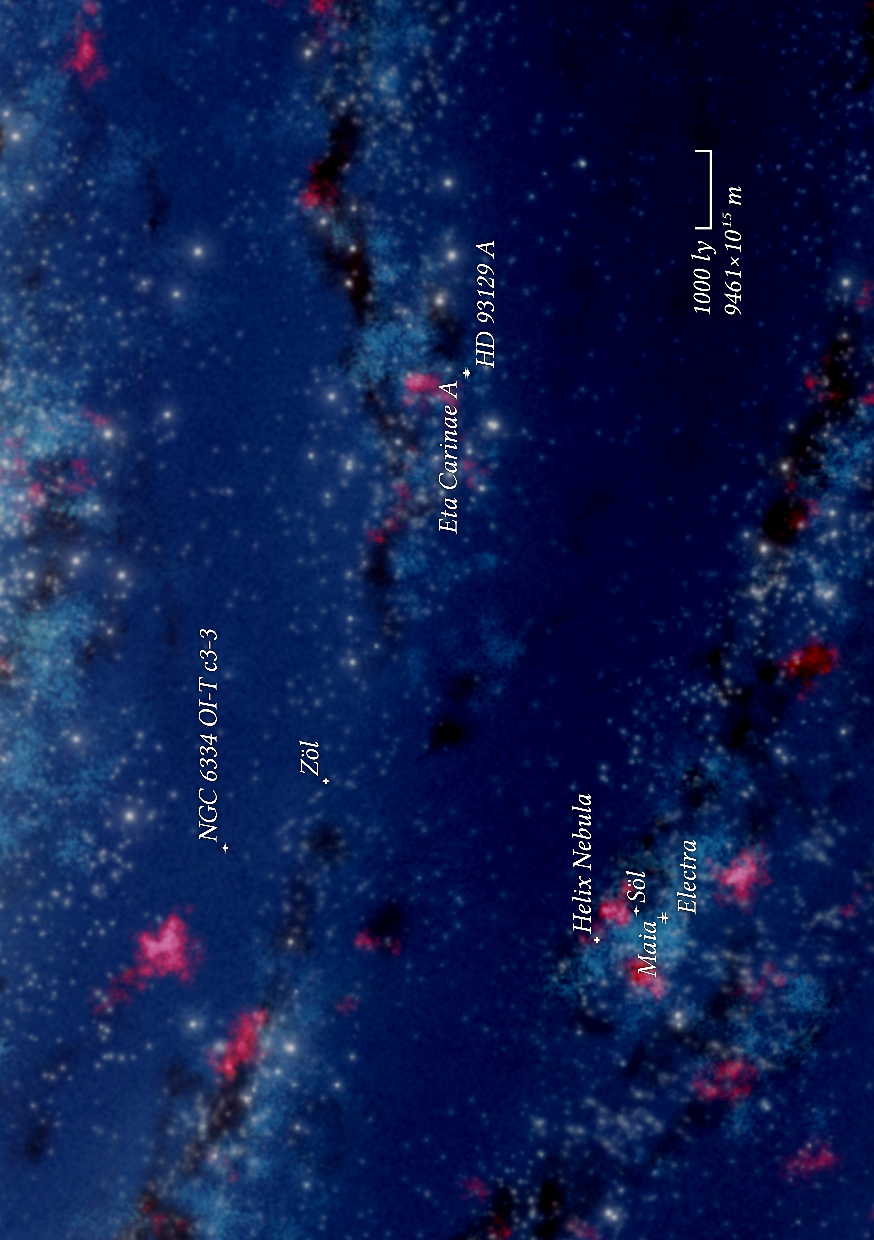
\includepdf[pages=-]{z-include-galaxyzoom-a5.pdf}


\chapter{Titelmelodie}

\begin{figure}[p]
    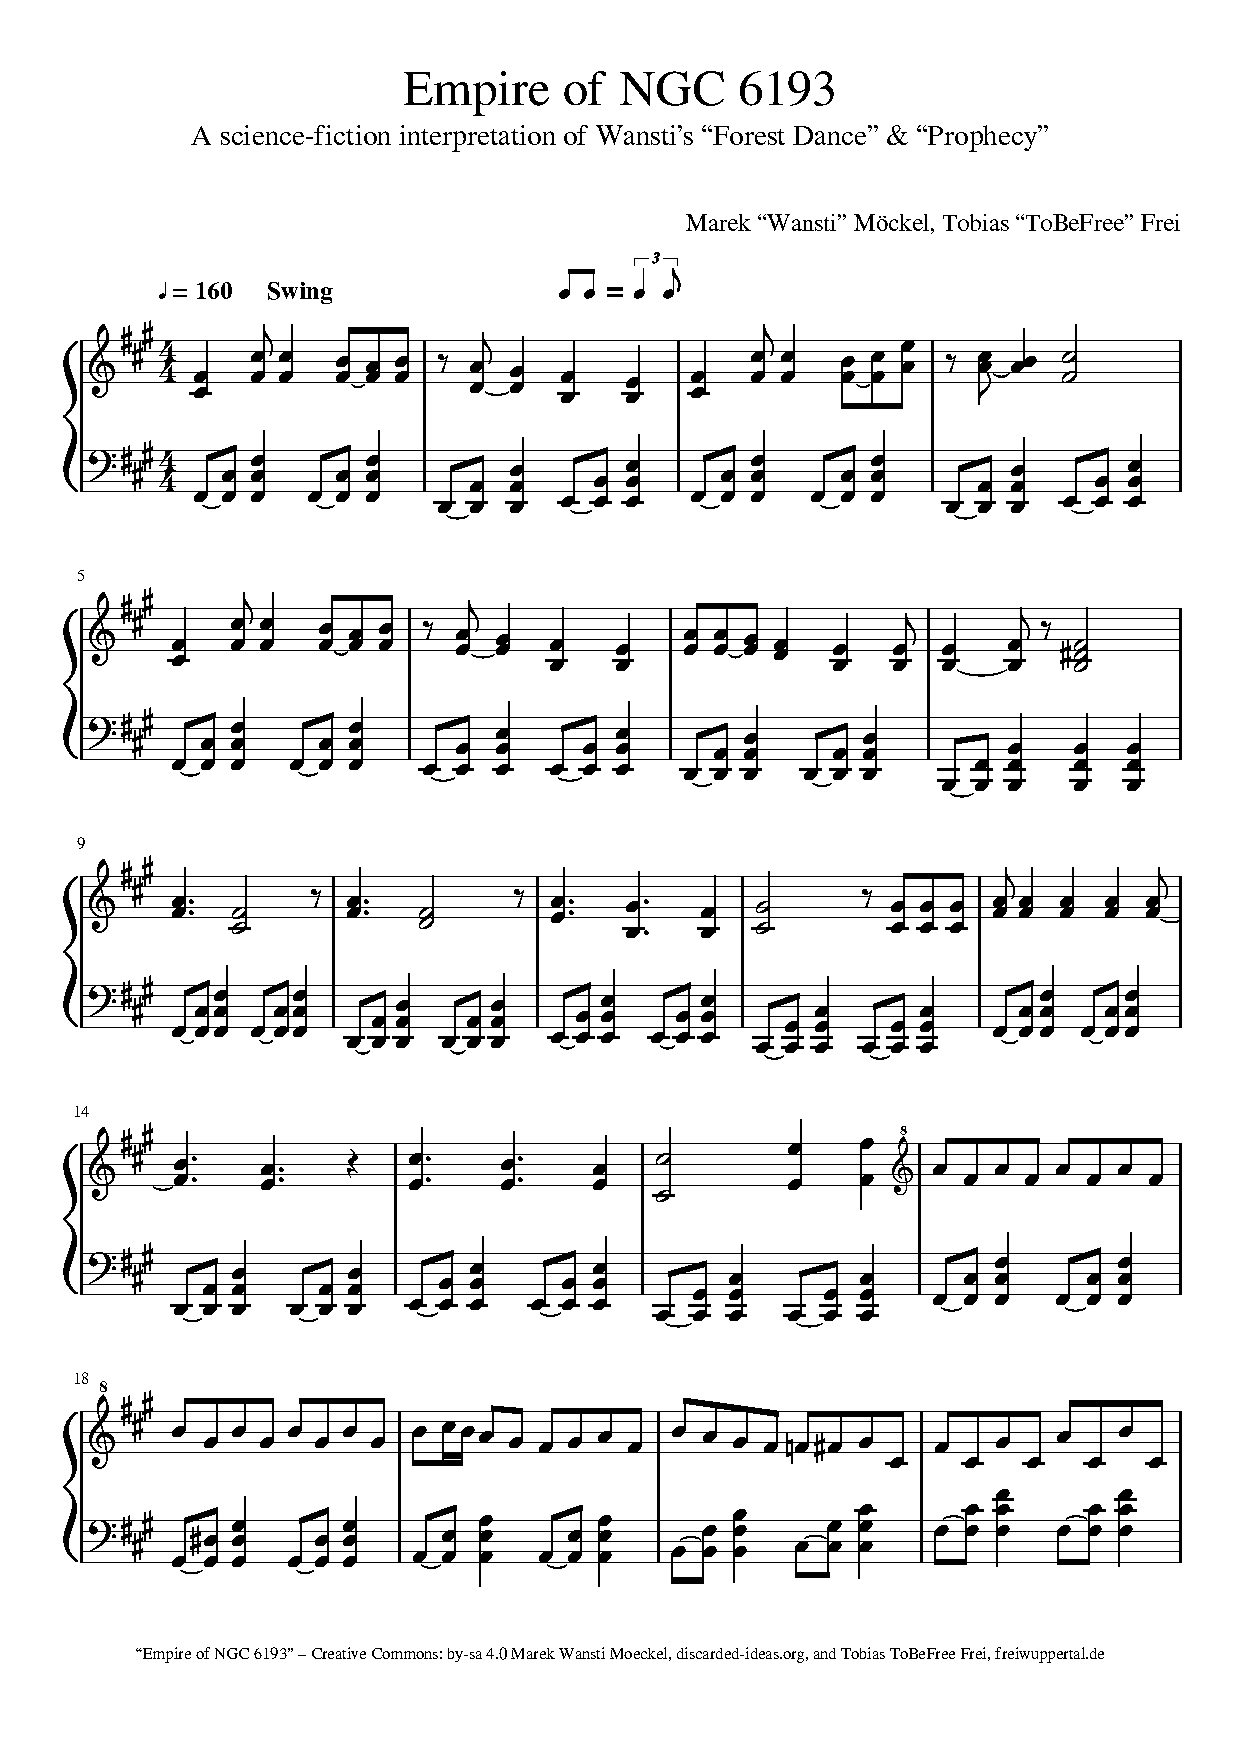
\includegraphics[width=\textwidth, page=1]{z-include-ia3theme.pdf}
\end{figure}

\begin{figure}[p]
    \includegraphics[width=\textwidth, page=2]{z-include-ia3theme.pdf}
\end{figure}

\begin{figure}[p]
    \includegraphics[width=\textwidth, page=3]{z-include-ia3theme.pdf}
\end{figure}


\chapter{Musikliste}

\textbf{Für Filmproduzenten, Träumer und Multitasking-Genies.}

\begin{itemize}
    \item Falls Du ernsthaft einen Film zu diesem Buch drehen möchtest.
    \item Falls Du das gesamte Buch bereits ausgelesen hast und die genannten Lieder vielleicht noch nicht kennst. Höre die Lieder und stelle Dir dabei die Szenen vor. Wenn es schon keinen IA-Film gibt, kannst Du wenigstens einen Film in deinem Kopf laufen lassen.
    \item Falls Du beim Lesen Musik hören möchtest, die zur aktuellen Szene passt.
\end{itemize}

Diese Liste wurde von Tobias Frei zusammengestellt und impliziert keinerlei Unterstützung oder Befürwortung durch die Komponisten der Lieder. Eines Tages wird jedes dieser Lieder in die Gemeinfreiheit übergehen; der genaue Zeitpunkt hängt von verschiedenen Gesetzen ab.

\begin{enumerate}
    \item Titelmelodie:\\ »Empire of NGC 6193«\\ Tobias »ToBeFree« Frei, Marek »Wansti« Möckel
    \item \textbf{Teil 1: Krieg im Carinanebel.}\\ Intromelodie / Prolog:\\ »Running Wild«~– Airbourne
    \item Wiedersehen mit den vier Abenteurern:\\ »Shoog Shoog«~– The Hu
    \item Relativistischer Asteroidenparcours:\\ »It’s My Life«~– Bon Jovi
    \item Trumpler 14 in Sicht:\\ »Stay Away«~– Nirvana
    \item Zwischen O-Sternen durch ein Strahlenmeer:\\ »Far Far Away«~– Battle Beast
    \item Kühlende Tauchstation:\\ »Azitmuth«~– Jason Shaw (Audionautix)
    \item Orakel lässt sich nicht aus der Ruhe bringen:\\ »Mountain Sun«~– Jason Shaw (Audionautix)
    \item Wasserflucht:\\ »Blue Boundary«~– World Order (die Band ist vor allem für ihre Tanzvideos bekannt)
    \item P-2255 am braunen Zwerg:\\ »My Prerogative«~– Robert Barisford Brown (Bobby Brown)
    \item Der Schlüssellochnebel:\\ »More«~– The Sisters of Mercy
    \item 2001:\\ »An der schönen blauen Donau«~– Johann Baptist Strauss II
    \item Kochsendung im Dunkeln:\\ »I’m Outta Love«~– Anastacia Lyn Newkirk
    \item Doppelkopf per Funk:\\ »Jolene«~– Dolly Rebecca Parton
    \item Reise zum Mittelpunkt des Nebels:\\ »Lucretia My Reflection«~– The Sisters of Mercy
    \item Kollisionsalarm:\\ »Hot Mess«~– Jason Shaw (Audionautix)
    \item Durchbruch mit Laserkraft:\\ »Up In Flames«~– Icon for Hire
    \item Allmächtiger Alderson:\\ »Salvation«~– In This Moment
    \item Jagd auf fünf Ameisen:\\ »Roots«~– In This Moment
    \item Licht über Lumina:\\ »Nightfall«~– Xandria
    \item Notruf in der Nacht:\\ »Stand My Ground«~– Within Temptation
    \item Sammlung der Untersuchungsflotte:\\ »Larger Than Life«~– Backstreet Boys, oder:\\ »Johnny Boy«~– Santiano
    \item Brückengespräche:\\ »Sonic~Robo~Blast~2~v2.2: Castle~Eggman~Zone, Act~1«~– DrTapeworm und CobaltBW, Sonic~Team~Junior
    \item Lagebesprechung beim Schachspiel:\\ »Ectoplasm«~– Jason Shaw (Audionautix)
    \item Historische Mutmaßungen:\\ »Cloud Nine«~– Evanescence
    \item Ankunft im Lux-System:\\ »In the Middle of the Night«~– Within Temptation
    \item Rettung und Flucht vom Lichtplaneten:\\ »The Silence«~– Manchester Orchestra
    \item Drei Wochen Strahlenschauer:\\ »Amigo«~– Bright White Lightning
    \item Mit Hoffnung durch den Felswall:\\ »Victoria’s Secret«~– Sonata Arctica
    \item Energiephysik:\\ »Guilt Is A Useless Emotion«~– New Order
    \item Erbsendose in der Funkstille:\\ »Too Close«~– Alex Clare
    \item Priorität 110:\\ »Life (12″ Mix)«~– Nestor Alexander Haddaway
    \item Nögnög unter Millionenbeschuss:\\ »Mechanicals«~– Rage of Light
    \item Letzte Besprechung vor dem Rückflug:\\ »Amaranth«~– Nightwish
    \item Berichte aus dem Helixnebel:\\ »Ohm«~– Jason Shaw (Audionautix)
    \item Die Mondlichtung:\\ »Silver Moonlight«~– Within Temptation
    \item Kritikstunde:\\ »Left Outside Alone«~– Anastacia Lyn Newkirk
    \item Tisiphönes Feuerbefehl:\\ »Lady of Worlds«~– Miracle of Sound
    \item Riesige Weltraumschlacht gegen die Roboter:\\ »The Last Frontier«~– Keldian
    \item Dreizehntausend Kilometer Stapelstart:\\ »Irresistible«~– Fall Out Boy
    \item Das Ende von Nögnög Zwölf:\\ »The Angels Weep«~– Jason Shaw (Audionautix)
    \item Alexandras Abschiedsbrief:\\ »Believe«~– Arven
    \item Ausflug zur Erde:\\ »The Way I Live My Life«~– Iris
    \item Technologiesprung:\\ »Lullaby«~– Johannes Brahms
    \item Selbstentlassung aus einem leeren Krankenhaus:\\ »Sugar«~– Robin Schulz
    \item Straßenverkehr:\\ »Transportation«~– Jason Shaw (Audionautix)
    \item Schnitzeljagd im All:\\ »Saving Time«~– Iris
    \item Das Ende von Hönüktün Fünf:\\ »The Angels Weep«~– Jason Shaw (Audionautix)
    \item PHÖNIX-Titelmelodie:\\ »The Phoenix«~– Fall Out Boy
    \item Mit dem Türbö Tächyön 1033 in das Mechanische Reich:\\ »Ghost Love Score«~– Nightwish
    \item Wiedersehen auf einem Berg:\\ »Twilight«~– Iris
    \item Das verlassene Verwaltungsgebäude:\\ »Clouds«~– Hugo Kant featuring Astrid Engberg
    \item Archäologiekritik:\\ »This Must Be The Place I Waited Years To Leave«~– Pet Shop Boys
    \item Erkunderische Ziellosigkeit:\\ »Oriental Haze«~– Tangerine Dream
    \item Die Geisterstadt:\\ »Ride on the Ray«~– Tangerine Dream
    \item Treppenlauf in Hochhaus 32:\\ »Sonic~Robo~Blast~2~v2.2: Techno~Hill~Zone, Act~2«~– Stuf und CobaltBW, Sonic~Team~Junior
    \item Kalte Rache:\\ »Marian«~– The Sisters Of Mercy
    \item Etage 67:\\ »The Catalyst«~– Linkin Park
    \item Flucht und hohe Rückkehr:\\ »Whisper«~– Evanescence
    \item Moralische Nachbetrachtung:\\ »If Everyone Cared«~– Nickelback
    \item Etage 103:\\ »Push the Button«~– Amy Lee
    \item Einsamer Passagierbahnhof:\\ »Time«~– Pink Floyd
    \item Leerfahrt:\\ »Barrel of a Gun«~– Depeche Mode
    \item Abrechnung:\\ »Milk and Honey«~– Delain
    \item Willkommen im Dunkelwald:\\ »Ohm«~– Jason Shaw (Audionautix)
    \item Zusammenbruch und Paradies:\\ »Sonic~Robo~Blast~2~v2.2: Black~Hole~Zone«~– RedXVI und CobaltBW, Sonic~Team~Junior
    \item Lagebetrachtung zwischen Ruinen:\\ »Sonic~Robo~Blast~2~v2.2: Aerial~Garden~Zone«~– RedXVI und CobaltBW, Sonic~Team~Junior
    \item Rückflug:\\ »Castle of Glass«~– Linkin Park
    \item \textbf{Teil 2: Die Zeitreise.}\\ Intromelodie / Prolog:\\ »Act Three«~– Jason Shaw (Audionautix)
    \item Ungeladener Gast:\\ »Walking in My Shoes«~– Depeche Mode
    \item Rückkehr nach Örz:\\ »Back In The Game«~– Airbourne
    \item Wiedersehensfest im Park:\\ »Counting Stars«~– OneRepublic
    \item Regenbogen:\\ »Nothing Like The Rain«~– 2 Unlimited
    \item Der Wanderer:\\ »The Visitors«~– ABBA
    \item Auf Wiedersehen, orangener Stern:\\ »Slow Farewell«~– Raphael Lake and Royal Baggs
    \item SETI und SOTI:\\ »Könnt ihr mich hören (MTV Unplugged)«~– Santiano
    \item Die Suche nach TMPE:\\ »Useless«~– Depeche Mode
    \item Beginn der Zeitreise:\\ »Flight of the Silverbird«~– Two Steps From Hell
    \item Der Weg zum Raumhafen:\\ »Way Down We Go«~– Kaleo
    \item Zwischenstopp Erde:\\ »Sleepwalkers Dream«~– Delain
    \item Eine Studie in Infrarot:\\ »Ribbons«~– The Sisters of Mercy
    \item Nüggäts letzte Flucht:\\ »My Favourite Game«~– The Cardigans
    \item Nüggät vor Gericht:\\ »Outlaw«~– The Phantoms
    \item Auf Bäumen in der Vergangenheit:\\ »The Voyage«~– Jason Shaw (Audionautix)
    \item Der Türbö Tächyön:\\ »True Faith«~– New Order
    \item Startvorbereitungen und Abflug von der Erde:\\ »Medley«~– Delain
    \item Das Archiv des Imperiums:\\ »See Me In Shadow«~– Delain
    \item Anflug auf Dönkwön II:\\ »Sometimes«~– Erasure
    \item Krönöhr Mäk:\\ »The Grey«~– Icon for Hire
    \item Wortgefecht zwischen yury und SOTI:\\ »Look Who’s Talking«~– Dr. Alban
    \item Urlaubsflug zu den Plejaden:\\ »Supernova«~– IMPP
    \item Kältephänomen im Hintergrund:\\ »When You Don't See Me«~– The Sisters of Mercy
    \item Elektra VI:\\ »United We Groove«~– Jason Shaw (Audionautix)
    \item Verlorenes Gold:\\ »Pech oder Glück«~– dArtagnan
    \item SOTI und SOTI:\\ »Life's What You Make It«~– Talk Talk
    \item Reset:\\ »Back In The Loop«~– E-Type
    \item Abschied von Toronto:\\ »C’est la vie«~– dArtagnan
    \item Ein alter Kamin:\\ »Primavera«~– Ludovico Einaudi
    \item Oldtimer aus dem Untergrund:\\ »Stronger Than You Think«~– Fireflight
    \item Rückkehr zum Helixnebel:\\ »Valhalla Calling«~– Miracle of Sound
    \item Eintritt zur Burg:\\ »Home«~– Depeche Mode
    \item Die Geschichte der Äöüzz, erster Gang:\\ »People Are People«~– Depeche Mode
    \item Die Geschichte der Äöüzz, zweiter Gang:\\ »Meer aus Tränen«~– Versengold
    \item Die Geschichte der Äöüzz, Nachtisch:\\ »Die wilde Jagd«~– Versengold
    \item Ankunft im Maia-System:\\ »Happy Now?«~– No Doubt
    \item Exzessive Gravitation:\\ »I Am All of Me«~– Crush 40
    \item Konfrontation der Giganten:\\ »They Catch Secrets«~– Camouflage
    \item Zerbrochene Träume:\\ »Deine Zweifel (Piano Version)«~– Max Giesinger
    \item Outro:\\ »Emerald«~– Zabutom
    \item \textbf{Teil 3: Bonusmaterial.}\\ Postskriptum:\\ »Freestate«~– Depeche Mode
    \item Zeitrechnung der Äöüzz:\\ »Time«~– Pink Floyd
    \item Das Python-Skript:\\ »Chiptune«~– Dubmood
    \item Kleines Lexikon und Bildquellen:\\ »Law and Order Theme«~– Mike Post
    \item Buchlizenz:\\ »Lieder der Freiheit (Live: Waldbühne Berlin 2016)«~– Santiano
\end{enumerate}


\chapter{Zeitrechnung der Äöüzz}

Die Zeitrechnung der Menschen auf Örs wird als UTC-Zeitrechnung (von »Coordinated Universal Time«) bezeichnet. Für die Abkürzung »UTC« haben sich die Menschen übrigens entschieden, um weder Französisch noch Örslängü zu bevorzugen. Außerhalb der Erde wird diese Zeitrechnung nicht genutzt.

Auf jedem Planeten der Äöüzz-Wirtschaftsvereinigung gilt die ÄÜC-Zeitrechnung. Es gibt keine Zeitzonen; der Zeitbegriff ist überall identisch. Die wissenschaftliche Definition wird nicht durch Schaltsekunden oder ähnliche Regelungen an historische Begriffsherkunften angepasst. Auf Örz und Planeten mit ähnlichen Rotationsgeschwindigkeiten orientieren sich die Arbeitszeiten am natürlichen Tageslicht; bei starker Abweichung verwendet die Bevölkerung künstliche Lichtquellen, um einen örzähnlichen Tagesrhythmus herzustellen. Die extremste Form solcher Abweichung ist die »gebundene Rotation« mancher Himmelskörper, auf denen keine natürlichen Tageszeiten existieren.

Der Name des Zeitsystems »ÄÜC« ist eine Abkürzung für »Ännö Ürbizz Cönditä«, abgeleitet aus dem lateinischen »anno urbis conditae«, »im Jahr der Stadtgründung«. Diese Abkürzung wird Jahreszahlen nachgestellt, beispielsweise als »1984 ÄÜC«.

Die vollständige Zeitdarstellung der Äöüzz für ÄÜC-Daten ist »Örzbit-Örzmön-Örzröt Örzklünk:Örzkläk:Örzklök ÄÜC«. Alle sechs Darstellungsfelder beginnen der mathematischen Einfachheit halber bei 0, anders als die mit 1 beginnende Monats- und Tagesnummerierung der UTC-Zeitrechnung. UTC-Daten werden als »JJJJ-MM-TT HH:MM:SS UTC« dargestellt. Kürzung an beiden Enden ist möglich, aber die Reihenfolge darf nie vertauscht werden.

Die ÄÜC-Begriffsdefinitionen lauten:

\begin{itemize}
    \item \textbf{Örzklök}, n., Plural Örzklöks, ugs. Klök/Klöks:\\ Ein Örzklök ist das 4×7¹¹-fache der Periodendauer der Strahlung, die beim Übergang zwischen den beiden Hyperfeinstrukturniveaus des Grundzustands eines Cäsium-133-Atoms entsteht. Es gilt daher:\\ 1 Örzklök = (7909306972 / 9192631770) Sekunden ≈ 0.8603 Sekunden.
    \item \textbf{Örzkläk}, n., Plural Örzkläks, ugs. Kläk/Kläks:\\ Ein Örzkläk entspricht\\ 7² Örzklöks = 49 Örzklöks. Es gilt daher:\\ 1 Örzkläk = 49 × (7909306972 / 9192631770) Sekunden ≈ 42 Sekunden ≈ 0.7027 Minuten.
    \item \textbf{Örzklünk}, n., Plural »Örzklünks«, ugs. Klünk/Klünks:\\ Ein Örzklünk entspricht\\ 7⁴ Örzklöks = 2401 Örzklöks = 7² Örzkläks. Es gilt daher:\\ 1 Örzklünk = 2401 × (7909306972 / 9192631770) Sekunden ≈ 2066 Sekunden ≈ 34 Minuten ≈ 0.5738 Stunden.
    \item \textbf{Örzröt}, n., Plural Örzröts, ugs. Röt/Röts:\\ Ein Örzröt entspricht\\ 7⁶ Örzklöks = 49 Örzklünks. Es gilt daher:\\ 1 Örzröt = 117649 × (7909306972 / 9192631770) Sekunden ≈ 101225 Sekunden ≈ 1687 Minuten ≈ 28 Stunden ≈ 1.1716 Tage.
    \item \textbf{Örzwök}, n., Plural Örzwöks, ugs. Wök/Wöks:\\ Ein Örzwök entspricht\\ 7⁷ Örzklöks = 7 Örzröts. Es gilt daher:\\ 1 Örzwök = 823543 × (7909306972 / 9192631770) Sekunden ≈ 708573 Sekunden ≈ 11810 Minuten ≈ 197 Stunden ≈ 8.201 Tage ≈ 1.1716 Wochen.
    \item \textbf{Örzmön}, n., Plural Örzmöns, ugs. Mön/Möns:\\ Ein Örzmön entspricht\\ 7⁸ Örzklöks = 7 Örzwöks = 49 Örzröts. Es gilt daher:\\ 1 Örzmön = 5764801 × (7909306972 / 9192631770) Sekunden ≈ 4960014 Sekunden ≈ 82667 Minuten ≈ 1378 Stunden ≈ 57.41 Tage ≈ 8.201 Wochen ≈ 1.9 × 30 Tage.
    \item \textbf{Örzbit}, n., Plural Örzbits:\\ Ein Örzbit entspricht\\ 7⁹ Örzklöks = 7 Örzmöns = 49 Örzwöks = 343 Örzröts. Es gilt daher:\\ 1 Örzbit = 40353607 × (7909306972 / 9192631770) Sekunden ≈ 34720097 Sekunden ≈ 578668 Minuten ≈ 9644 Stunden ≈ 402 Tage ≈ 1.1002 × 365.25 Tage.\\ Um eine Verwechslung mit binären Ziffern zu vermeiden, werden die Begriffe »Bit« und »Bits« nicht als Abkürzungen genutzt.
\end{itemize}

Der Beginn des ÄÜC-Kalenders ist definiert als der Beginn des irdischen Jahres »Minus 752« irdischer astronomischer Zeitrechnung. Es gilt daher grob:

\begin{itemize}
    \item Jahr x UTC\\ = (x+752)/(40353607×(7909306972/9192631770)/60/60/24/365.25) ÄÜC
    \item Jahr x ÄÜC\\ = x×40353607×(7909306972/9192631770)/60/60/24/365.25-752 UTC
\end{itemize}

Die sekundengenaue Umrechnung zwischen den beiden Datumsformaten wird durch Schaltjahre und unterschiedliche Monatslängen der irdischen Zeitrechnung verkompliziert: Wie viele Sekunden sind seit Beginn der Zeitrechnung vergangen? Für ÄÜC-Daten lässt sich diese Frage durch eine statische Formel beantworten, bei UTC-Angaben muss die Anzahl der Sekunden pro Jahr inklusive Schaltsekunden berechnet werden. Verzichtet man auf die Berücksichtigung der Schaltsekunden, kann zumindest ein einfacher Algorithmus die Schaltjahre berücksichtigen.

Beispieldaten:

\begin{itemize}
    \item -752-01-01, 00:00:00 UTC = -752 UTC\\ = 0 ÄÜC = 0000-00-00, 00:00:00 ÄÜC
    \item -047-01-01, 00:00:00 UTC = -47 UTC\\ ≈ 640.7716692 ÄÜC ≈ 640-5-19, 33:21:35 ÄÜC
    \item 1430-11-14, 07:08:34 UTC ≈ 1430.8693085 UTC\\ ≈ 1984.0000000 ÄÜC ≈ 1984-00-00, 00:00:00 ÄÜC
    \item 2012-07-09, 14:10:01 UTC ≈ 2012.5207385 UTC\\ ≈ 2512.6617424 ÄÜC ≈ 2512-04-30, 47:44:15 ÄÜC
    \item 2019-04-01, 00:00:00 UTC ≈ 2019.2465753 UTC\\ ≈ 2518.7744500 ÄÜC ≈ 2518-05-20, 31:08:42 ÄÜC
    \item 2021-04-01, 00:00:00 UTC ≈ 2021.2465753 UTC\\ ≈ 2520.5935232 ÄÜC ≈ 2520-04-07, 28:16:44 ÄÜC
    \item 2022-04-01, 00:00:00 UTC ≈ 2022.2465753 UTC\\ ≈ 2521.5018156 ÄÜC ≈ 2521-03-25, 06:00:37 ÄÜC
    \item 2046-06-09, 02:13:37 UTC ≈ 2046.4358707 UTC\\ ≈ 2543.4876995 ÄÜC ≈ 2543-03-20, 13:37:25 ÄÜC
    \item 4669-02-05, 00:07:01 UTC ≈ 4669.0959038 UTC\\ ≈ 4927.2125378 ÄÜC ≈ 4927-01-23, 44:06:00 ÄÜC
\end{itemize}

\section{Kalender mit Umrechnungshinweisen}

Ohne Computerskript ist die Umrechnung zwar aufwendig, aber durchführbar. Als klassisches Hilfsmittel kann ein Kalender dienen, in dem die Anzahl der Tage seit Jahresbeginn dargestellt wird.

\subsection{Irdischer UTC-Kalender}

Die Nachkommastellen der UTC-Jahreszahl sind »x/365« in Nicht-Schaltjahren und »x/366« in Schaltjahren, wobei x der Anzahl der seit Jahresbeginn vergangenen Tage entspricht. Diese Anzahl ergibt sich durch Addition der Tageszahl im Datum und der Anzahl der Tage aller vorhergehenden Monate. Zwei negativ wirkende Effekte sind zu beachten: Die Tageszahlen im aktuellen Monat beginnen mit 1 statt 0, und der erste Tag des Jahres ist der »erste« Januar. Auf eine März-Tageszahl muss daher in einem Nicht-Schaltjahr 31+28-1-1 = 57 addiert werden, um die Anzahl der bis dahin vergangenen Tage zu errechnen. Am 15. März sind 31+28+15-1-1 = 73 Tage im laufenden Jahr vergangen. Der Beginn des 15. März 2019 UTC ist exakt »2019.2 UTC«.

\begin{itemize}
\item \textbf{Januar} (+0 Tage):\\ xxxx-01-01 UTC bis xxxx-01-31 UTC
\item \textbf{Februar} (+31 Tage):\\ xxxx-02-01 UTC bis xxxx-02-28 UTC (Nicht-Schaltjahr), oder\\ xxxx-02-01 UTC bis xxxx-02-29 UTC (Schaltjahr)
\item \textbf{März} (+59/+60 Tage):\\ xxxx-03-01 UTC bis xxxx-03-31 UTC
\item \textbf{April} (+90/+91 Tage):\\ xxxx-04-01 UTC bis xxxx-04-30 UTC
\item \textbf{Mai} (+120/+121 Tage):\\ xxxx-05-01 UTC bis xxxx-05-31 UTC
\item \textbf{Juni} (+151/+152 Tage):\\ xxxx-06-01 UTC bis xxxx-06-30 UTC
\item \textbf{Juli} (+181/+182 Tage):\\ xxxx-07-01 UTC bis xxxx-07-31 UTC
\item \textbf{August} (+212/+213 Tage):\\ xxxx-08-01 UTC bis xxxx-08-31 UTC
\item \textbf{September} (+243/+244 Tage):\\ xxxx-09-01 UTC bis xxxx-09-30 UTC
\item \textbf{Oktober} (+273/+274 Tage):\\ xxxx-10-01 UTC bis xxxx-10-31 UTC
\item \textbf{November} (+304/+305 Tage):\\ xxxx-11-01 UTC bis xxxx-11-30 UTC
\item \textbf{Dezember} (+334/+335 Tage):\\ xxxx-12-01 UTC bis xxxx-12-31 UTC
\end{itemize}

\subsection{Äöüzz-ÄÜC-Kalender}

Der Kalender der Äöüzz ist dankenswerterweise deutlich simpler gehalten. Da die Tageszahlen bei Null beginnen, ist keine Subtraktion erforderlich. Auf eine Tageszahl im dritten Örzmön muss daher nur 49+49 addiert werden, um die Anzahl der bis dahin vergangenen Tage zu berechnen.

\begin{itemize}
\item Örzmön 0 (+0 Tage):\\ xxxx-00-00 ÄÜC bis xxxx-00-48 ÄÜC
\item Örzmön 1 (+49 Tage):\\ xxxx-01-00 ÄÜC bis xxxx-01-48 ÄÜC
\item Örzmön 2 (+98 Tage):\\ xxxx-02-00 ÄÜC bis xxxx-02-48 ÄÜC
\item Örzmön 3 (+147 Tage):\\ xxxx-03-00 ÄÜC bis xxxx-03-48 ÄÜC
\item Örzmön 4 (+196 Tage):\\ xxxx-04-00 ÄÜC bis xxxx-04-48 ÄÜC
\item Örzmön 5 (+245 Tage):\\ xxxx-05-00 ÄÜC bis xxxx-05-48 ÄÜC
\item Örzmön 6 (+294 Tage):\\ xxxx-06-00 ÄÜC bis xxxx-06-48 ÄÜC
\end{itemize}

\section{Skript zur Umrechnung}

Geschrieben in Python 3.9, ohne Berücksichtigung von Schaltsekunden.

\begin{tiny}
\begin{ttfamily}
\begin{verbatim}
#!/bin/python3
# AeUeCalendar, urspruenglich erstellt fuer die Infinite Adventures
# Dieses Python-Skript ist gemeinfrei / public domain / CC0.
# Tobias Frei, 2022

# This is free and unencumbered software released into the public domain.

# THE SOFTWARE IS PROVIDED "AS IS", WITHOUT WARRANTY OF ANY KIND,
# EXPRESS OR IMPLIED, INCLUDING BUT NOT LIMITED TO THE WARRANTIES OF
# MERCHANTABILITY, FITNESS FOR A PARTICULAR PURPOSE AND NONINFRINGEMENT.
# IN NO EVENT SHALL THE AUTHORS BE LIABLE FOR ANY CLAIM, DAMAGES OR
# OTHER LIABILITY, WHETHER IN AN ACTION OF CONTRACT, TORT OR OTHERWISE,
# ARISING FROM, OUT OF OR IN CONNECTION WITH THE SOFTWARE OR THE USE OR
# OTHER DEALINGS IN THE SOFTWARE.

TF_SECONDS_PER_OERZKLOEK: float = 7909306972 / 9192631770
TF_SECONDS_PER_OERZBIT: float = 343 * 49 * 49 * 49 * TF_SECONDS_PER_OERZKLOEK


def tf_convert_utc_auc(tf_in_date: dict) -> dict:
    # UTC -> AUC
    tf_out_date: dict[str, int] = {
        "year": -5000,
        "month": 1,
        "day": 1,
        "hour": 0,
        "minute": 0,
        "second": 0
    }

    if (((tf_in_date["year"] % 4 == 0)
        and (tf_in_date["year"] % 100 != 0))
            or (tf_in_date["year"] % 400 == 0)):
        # leap year
        tf_calendar: list[int] = [31, 29, 31, 30, 31, 30, 31, 31, 30, 31, 30, 31]
        tf_current_year_days: int = 366
    else:
        tf_calendar: list[int] = [31, 28, 31, 30, 31, 30, 31, 31, 30, 31, 30, 31]
        tf_current_year_days: int = 365
    tf_current_year_hours: int = tf_current_year_days * 24
    tf_current_year_minutes: int = tf_current_year_hours * 60
    tf_current_year_seconds: int = tf_current_year_minutes * 60
    tf_past_days: int = 0
    # Months start at 1, so "1" means no month has passed and "12" means 11 have passed
    tf_past_months: int = tf_in_date["month"] - 1
    for x in tf_calendar:
        if tf_past_months < 1:
            break
        tf_past_days += x
        tf_past_months -= 1

    # Days start at 1 as well
    tf_in_year_decimal: float = tf_in_date["year"]
    tf_in_year_decimal += (tf_past_days + tf_in_date["day"] - 1) / tf_current_year_days
    tf_in_year_decimal += tf_in_date["hour"] / tf_current_year_hours
    tf_in_year_decimal += tf_in_date["minute"] / tf_current_year_minutes
    tf_in_year_decimal += tf_in_date["second"] / tf_current_year_seconds
    tf_out_year_decimal: float = tf_seconds_ab_urbe_condita(tf_in_date["year"])
    tf_out_year_decimal += (tf_past_days + tf_in_date["day"] - 1) * 24 * 60 * 60
    tf_out_year_decimal += tf_in_date["hour"] * 60 * 60
    tf_out_year_decimal += tf_in_date["minute"] * 60
    tf_out_year_decimal += tf_in_date["second"]
    tf_out_year_decimal /= TF_SECONDS_PER_OERZBIT

    # Exporting to AUC is simple as there are no leap years,
    # each month has the same length and all fields start at 0.
    tf_rest = tf_out_year_decimal  # e.g. 2033.4029528
    tf_out_date["year"] = int(tf_out_year_decimal // 1)  # e.g. 2033
    tf_rest -= tf_out_date["year"]  # e.g. 0.4029528
    tf_out_date["month"] = int((tf_rest * 7) // 1)  # AUC y = 7 M
    tf_rest -= tf_out_date["month"] / 7
    tf_out_date["day"] = int((tf_rest * 343) // 1)  # AUC y = 343 d
    tf_rest -= tf_out_date["day"] / 343
    tf_out_date["hour"] = int((tf_rest * 343 * 49) // 1)  # AUC d = 49 h
    tf_rest -= tf_out_date["hour"] / (343 * 49)
    tf_out_date["minute"] = int((tf_rest * 343 * 49 * 49) // 1)  # AUC h = 49 m
    tf_rest -= tf_out_date["minute"] / (343 * 49 * 49)
    tf_out_date["second"] = int((tf_rest * 343 * 49 * 49 * 49) // 1)  # AUC m = 49 s
    tf_rest -= tf_out_date["second"] / (343 * 49 * 49 * 49)

    return tf_out_date


def tf_seconds_ab_urbe_condita(tf_in_year: int) -> int:
    # How many seconds have passed
    # between the start of "-752" and the start of the current year?
    tf_out_seconds: int = 0
    tf_loop_begin: int = min(tf_in_year, (-752))
    tf_loop_end: int = max(tf_in_year, (-752))
    tf_loop_sign: int = (tf_in_year > (-752)) - (tf_in_year < (-752))
    for y in range(tf_loop_begin, tf_loop_end):
        if ((y % 4 == 0) and (y % 100 != 0)) or (y % 400 == 0):
            # leap year
            tf_out_seconds += 366 * 24 * 60 * 60
        else:
            tf_out_seconds += 365 * 24 * 60 * 60
    return tf_loop_sign * tf_out_seconds


def main() -> None:
    tf_calendar_main: list[int] = [31, 29, 31, 30, 31, 30, 31, 31, 30, 31, 30, 31]
    tf_in_date: dict[str, int] = {
        "year": -999,
        "month": 1,
        "day": 1,
        "hour": 0,
        "minute": 0,
        "second": 0
    }

    while tf_in_date["year"] <= 3000:
        tf_out_date = tf_convert_utc_auc(tf_in_date)
        tf_out_string = str(int(tf_in_date["year"])).zfill(4) + "-"
        tf_out_string += str(int(tf_in_date["month"])).zfill(2) + "-"
        tf_out_string += str(int(tf_in_date["day"])).zfill(2) + ", "
        tf_out_string += str(int(tf_in_date["hour"])).zfill(2) + ":"
        tf_out_string += str(int(tf_in_date["minute"])).zfill(2) + ":"
        tf_out_string += str(int(tf_in_date["second"])).zfill(2) + " UTC = "
        tf_out_string += str(int(tf_out_date["year"])).zfill(4) + "-"
        tf_out_string += str(int(tf_out_date["month"])).zfill(2) + "-"
        tf_out_string += str(int(tf_out_date["day"])).zfill(2) + ", "
        tf_out_string += str(int(tf_out_date["hour"])).zfill(2) + ":"
        tf_out_string += str(int(tf_out_date["minute"])).zfill(2) + ":"
        tf_out_string += str(int(tf_out_date["second"])).zfill(2) + " ÄÜC"
        print(tf_out_string)

        if (((tf_in_date["year"] % 4 == 0)
            and (tf_in_date["year"] % 100 != 0))
                or (tf_in_date["year"] % 400 == 0)):
            # leap year
            tf_calendar_main[1] = 29
        else:
            tf_calendar_main[1] = 28

        tf_in_date["hour"] += 1
        if tf_in_date["hour"] > 23:
            tf_in_date["hour"] = 0
            tf_in_date["day"] += 1
        if tf_in_date["day"] > tf_calendar_main[tf_in_date["month"] - 1]:
            tf_in_date["day"] = 1
            tf_in_date["month"] += 1
        if tf_in_date["month"] > 12:
            tf_in_date["month"] = 1
            tf_in_date["year"] += 1


if __name__ == "__main__":
    main()
\end{verbatim}
\end{ttfamily}
\end{tiny}


\chapter{Kleines Lexikon}

\begin{itemize}
    \item \textbf{15 Prozent:}\\ Lorentzfaktor der halben Lichtgeschwindigkeit (ca. 1.155 bei 0.5~c) minus Lorentzfaktor der Ruhe (1). Der Lorentzfaktor ist der Kehrwert der Wurzel von X, wenn man X als »1 minus quadrierte Geschwindigkeit-Lichtgeschwindigkeitstel« definiert. Er gibt an, wie stark sich die Zeitdilatation bei einer bestimmten Geschwindigkeit auswirkt. Zur Lichtgeschwindigkeit hin wird er unendlich groß.
    \item \textbf{4.6692:}\\ Feigenbaum-Konstante (Chaoskonstante) δ ≈ 4.6692016091
    \item \textbf{(16. Dezember) 1971:}\\ Annahme der Biowaffenkonvention durch die Vollversammlung der Vereinten Nationen
    \item \textbf{343:}\\ 7³
    \item \textbf{2401:}\\ 7⁴
    \item \textbf{3087:}\\ 7⁴+2×7³
    \item \textbf{ÄÜC:}\\ »Ännö Ürbizz Cönditä«. Siehe Bonus-Kapitel »Zeitrechnung der Äöüzz«.
    \item \textbf{ISG:}\\ IntärStällär Gräm, InterStellare Gewichtseinheit.\\ 1 ISG ist die Masse von 3×7²⁹ Silicium-28-Atomen. Daher gilt:\\ 1 ISG ≈ 0.4487593 Kilogramm.
    \item \textbf{Meter:}\\ Die Länge der Strecke, die das Licht im Vakuum während der Dauer von\\ 93802365/24195414063392012 Örzklöks\\ zurücklegt. Daher gilt:\\ 1 Lichtjahr = 9460730472580800 Meter.
    \item \textbf{»Mir ist kalt.«:}\\ Anspielung auf »Mir wird kalt«, die letzte Zeile des Liedes »Major~Tom« von Peter~Schilling.
    \item \textbf{Örzklök:}\\ Das 4×7¹¹-fache der Periodendauer der Strahlung, die beim Übergang zwischen den beiden Hyperfeinstrukturniveaus des Grundzustands eines Cäsium-133-Atoms entsteht. Daher gilt:\\ 1 Örzklök = (7909306972 / 9192631770) Sekunden,\\1 Örzklök ≈ 0.8603 Sekunden.
    \begin{itemize}
        \item \textbf{Örzkläk:}\\ 7² Örzklöks, ca. 42 Sekunden, ca. 0.7027 Minuten.
        \item \textbf{Örzklünk:}\\ 7⁴ Örzklöks, ca. 34 Minuten, ca. 0.5738 Stunden.
        \item \textbf{Örzröt:}\\ 7⁶ Örzklöks, ca. 28 Stunden, ca. 1.1716 Tage.
        \item \textbf{Örzwök:}\\ 7⁷ Örzklöks, ca. 8.201 Tage, ca. 1.1716 Wochen.
        \item \textbf{Örzmön:}\\ 7⁸ Örzklöks, ca. 57.41 Tage, ca. 8.201 Wochen, ca. 1.9 × 30 Tage.
        \item \textbf{Örzbit:}\\ 7⁹ Örzklöks, ca. 402 Tage, ca. 1.1002 × 365.25 Tage.
    \end{itemize}
    \item \textbf{Örztemp:}\\ Absolute Temperaturskala der Äöüzz. 1 Örztemp ist die thermodynamische Temperatur des Tripelpunktes des Wassers geteilt durch 7³. Daher gilt:\\ 1 Örztemp = (343/273.16) Kelvin.
    \item \textbf{»Wie eine Blume am Winterbeginn«:}\\ Zitat der ersten Zeile des Liedes »Ein bisschen Frieden« von Nicole~Hohloch.
\end{itemize}


\chapter{Bildquellen}

Alle verwendeten Bilder sind gemeinfrei. Die Verwendung der Bilder in diesem Roman impliziert keinerlei Unterstützung oder Befürwortung durch ihre Schöpfer.

\begin{itemize}
    \item \textbf{Blauer Carinanebel (Buchcover):} CC0-Lizenz / Public Domain.\\ Dylan O'Donnell, deography.com\\ »That means it’s free for you to use, now and forever. You don’t even have to credit me for it. […] Photography is not my job and I’d rather not kill any enthusiasm I have for it by accepting money for the obligation to take photos. So use them, by all means. You don’t have to credit me if you don’t want to, but I love seeing my work out there in the wild being used, mixed and remixed. Send me a link, I’d love to see what you do!« (https://deography.com/yes-its-free/\#, Abruf 2022-01-01)
    \item \textbf{Galaktische Karte:} CC0-Lizenz / Public Domain.\\ Alle galaktischen Kartenbilder basieren auf einem Bild von\\ NASA/JPL-Caltech/R. Hurt (SSC/Caltech). Abruf über Wikimedia Commons 2022-02-02.\\ https://commons.wikimedia.org/w/index.php?title=\\File:Ssc2008-10a1.tif\\\&oldid=481274511
    \item \textbf{Detailansichten des Carinanebels:} CC0-Lizenz / Public Domain.\\ NASA, ESA, N. Smith (University of California, Berkeley), and The Hubble Heritage Team (STScI/AURA); CTIO Image: N. Smith (University of California, Berkeley) and NOAO/AURA/NSF. Veröffentlicht 2007-04-27. Abruf über Wikimedia Commons 2022-02-02.\\ https://commons.wikimedia.org/w/index.php?title=\\File:NGC\_3372a-full.jpg\\\&oldid=598394981
    \item \textbf{Helixnebel:} CC0-Lizenz / Public Domain.\\ NASA/JPL-Caltech.\\ Veröffentlicht 2012-10-02. Abruf über Wikimedia Commons 2017-12-30.\\ https://commons.wikimedia.org/w/index.php?title=\\File:Helix\_Nebula\_-\_Unraveling\_at\_the\_Seams.jpg\\\&oldid=224022245
    \item \textbf{Homunkulusnebel:} CC0-Lizenz / Public Domain.\\ Eine gemeinfreie Kombination zweier gemeinfreier Bilder, zusammengestellt von Sumanch. Veröffentlicht 2008-04-24T22:36:07. Abruf über Wikimedia Commons 2022-02-02.\\ https://commons.wikimedia.org/w/index.php?title=\\File:EtaCarinae.jpg\\\&oldid=606714129
    \item \textbf{Homunkulusnebel, Teilbild 1:} CC0-Lizenz / Public Domain.\\ Jon Morse (University of Colorado) \& NASA Hubble Space Telescope. Veröffentlicht 1996-06-10. Abruf über Wikimedia Commons 2022-02-02.\\ https://commons.wikimedia.org/w/index.php?title=\\File:Eta\_Carinae.jpg\\\&oldid=614332543
    \item \textbf{Homunkulusnebel, Teilbild 2:} CC0-Lizenz / Public Domain.\\ J. Hester/Arizona state University \& NASA Hubble Space Telescope. Veröffentlicht 1994-01-14. Abruf über Wikimedia Commons 2022-02-02.\\ https://commons.wikimedia.org/w/index.php?title=\\File:Etacarinae-001.jpg\\\&oldid=139305478
    \item \textbf{Plejaden:} CC0-Lizenz / Public Domain.\\ NASA, ESA, AURA/Caltech, Palomar Observatory. Veröffentlicht 2007-04-27. Abruf über Wikimedia Commons 2022-02-02.\\ https://commons.wikimedia.org/w/index.php?title=\\File:Pleiades\_large.png\\\&oldid=620262214
\end{itemize}

Bei den Bildern in diesem Roman handelt es sich nicht um die exakten Originalbilder, sondern um Abwandlungen (Weißabgleich, Helligkeit, Kontrast, Sättigung, Schärfung, Zuschnitt etc.) erstellt durch Tobias Frei.

Für die Infinite Adventures erstellte Abwandlungen frei lizenzierter Werke wurden auf Wikimedia Commons hochgeladen und auf diese Weise an die Gemeinschaft zurückgegeben.


\chapter{Lizenz des Buchinhalts}

\textbf{Infinite Adventures 3 © by\\ Tobias Frei, infiniteadventures.de}

Dies ist eine offizielle Ausgabe der Infinite Adventures 3, herausgegeben von Tobias Frei. Veränderte Versionen und unautorisierte Nachdrucke müssen deutlich als solche erkennbar sein. Auch das Impressum muss angepasst werden, wenn das Dokument verändert wird.

Falls Du die Rechte in dieser Lizenz nutzen möchtest, musst Du sie vollständig gelesen und verstanden haben. Es genügt nicht, nur eine Zusammenfassung zu lesen. Aus diesem Grund wird in diesem Buch keine Zusammenfassung angeboten.

This novel is licensed under a Creative Commons Attribution-ShareAlike 4.0 International License.

You should have received a copy of the license along with this work. If not, see\\
https://creativecommons.org/licenses/by-sa/4.0/legalcode

You are required to actually read and understand the full text of the license, not a summary.

\begin{center}
    \large{\textbf{Creative Commons Attribution-ShareAlike 4.0 International Public License}}
\end{center}

By exercising the Licensed Rights (defined below), You accept and agree to be bound by the terms and conditions of this Creative Commons Attribution-ShareAlike 4.0 International Public License ("Public License"). To the extent this Public License may be interpreted as a contract, You are granted the Licensed Rights in consideration of Your acceptance of these terms and conditions, and the Licensor grants You such rights in consideration of benefits the Licensor receives from making the Licensed Material available under these terms and conditions.

\begin{center}
    \textbf{Section 1 -- Definitions.}
\end{center}

\begin{itemize}
    \item[a.] \textbf{Adapted Material} means material subject to Copyright and Similar Rights that is derived from or based upon the Licensed Material and in which the Licensed Material is translated, altered, arranged, transformed, or otherwise modified in a manner requiring permission under the Copyright and Similar Rights held by the Licensor. For purposes of this Public License, where the Licensed Material is a musical work, performance, or sound recording, Adapted Material is always produced where the Licensed Material is synched in timed relation with a moving image.
    \item[b.] \textbf{Adapter's License} means the license You apply to Your Copyright and Similar Rights in Your contributions to Adapted Material in accordance with the terms and conditions of this Public License.
    \item[c.] \textbf{BY-SA Compatible License} means a license listed at creativecommons.org/compatiblelicenses, approved by Creative Commons as essentially the equivalent of this Public License.
    \item[d.] \textbf{Copyright and Similar Rights} means copyright and/or similar rights closely related to copyright including, without limitation, performance, broadcast, sound recording, and Sui Generis Database Rights, without regard to how the rights are labeled or categorized. For purposes of this Public License, the rights specified in Section 2(b)(1)-(2) are not Copyright and Similar Rights.
    \item[e.] \textbf{Effective Technological Measures} means those measures that, in the absence of proper authority, may not be circumvented under laws fulfilling obligations under Article 11 of the WIPO Copyright Treaty adopted on December 20, 1996, and/or similar international agreements.
    \item[f.] \textbf{Exceptions and Limitations} means fair use, fair dealing, and/or any other exception or limitation to Copyright and Similar Rights that applies to Your use of the Licensed Material.
    \item[g.] \textbf{License Elements} means the license attributes listed in the name of a Creative Commons Public License. The License Elements of this Public License are Attribution and ShareAlike.
    \item[h.] \textbf{Licensed Material} means the artistic or literary work, database, or other material to which the Licensor applied this Public License.
    \item[i.] \textbf{Licensed Rights} means the rights granted to You subject to the terms and conditions of this Public License, which are limited to all Copyright and Similar Rights that apply to Your use of the Licensed Material and that the Licensor has authority to license.
    \item[j.] \textbf{Licensor} means the individual(s) or entity(ies) granting rights under this Public License.
    \item[k.] \textbf{Share} means to provide material to the public by any means or process that requires permission under the Licensed Rights, such as reproduction, public display, public performance, distribution, dissemination, communication, or importation, and to make material available to the public including in ways that members of the public may access the material from a place and at a time individually chosen by them.
    \item[l.] \textbf{Sui Generis Database Rights} means rights other than copyright resulting from Directive 96/9/EC of the European Parliament and of the Council of 11 March 1996 on the legal protection of databases, as amended and/or succeeded, as well as other essentially equivalent rights anywhere in the world.
    \item[m.] \textbf{You} means the individual or entity exercising the Licensed Rights under this Public License. Your has a corresponding meaning.
\end{itemize}

\begin{center}
    \textbf{Section 2 -- Scope.}
\end{center}

\begin{itemize}
    \item[a.] \textbf{License grant.}
    \begin{itemize}
        \item[1.] Subject to the terms and conditions of this Public License, the Licensor hereby grants You a worldwide, royalty-free, non-sublicensable, non-exclusive, irrevocable license to exercise the Licensed Rights in the Licensed Material to:
        \begin{itemize}
            \item[A.] reproduce and Share the Licensed Material, in whole or in part; and
            \item[B.] produce, reproduce, and Share Adapted Material.
        \end{itemize}
        \item[2.] \underline{Exceptions and Limitations}. For the avoidance of doubt, where Exceptions and Limitations apply to Your use, this Public License does not apply, and You do not need to comply with its terms and conditions.
        \item[3.] \underline{Term}. The term of this Public License is specified in Section 6(a).
        \item[4.] \underline{Media and formats; technical modifications allowed}. The Licensor authorizes You to exercise the Licensed Rights in all media and formats whether now known or hereafter created, and to make technical modifications necessary to do so. The Licensor waives and/or agrees not to assert any right or authority to forbid You from making technical modifications necessary to exercise the Licensed Rights, including technical modifications necessary to circumvent Effective Technological Measures. For purposes of this Public License, simply making modifications authorized by this Section 2(a)(4) never produces Adapted Material.
        \item[5.] \underline{Downstream recipients}.
        \begin{itshape}\begin{itemize}
            \item[A.] \underline{Offer from the Licensor -- Licensed Material}. Every recipient of the Licensed Material automatically receives an offer from the Licensor to exercise the Licensed Rights under the terms and conditions of this Public License.
            \item[B.] \underline{Additional offer from the Licensor -- Adapted Material}. Every recipient of Adapted Material from You automatically receives an offer from the Licensor to exercise the Licensed Rights in the Adapted Material under the conditions of the Adapter's License You apply.
            \item[C.] \underline{No downstream restrictions}. You may not offer or impose any additional or different terms or conditions on, or apply any Effective Technological Measures to, the Licensed Material if doing so restricts exercise of the Licensed Rights by any recipient of the Licensed Material.
        \end{itemize}\end{itshape}
        \item[6.] \underline{No endorsement}. Nothing in this Public License constitutes or may be construed as permission to assert or imply that You are, or that Your use of the Licensed Material is, connected with, or sponsored, endorsed, or granted official status by, the Licensor or others designated to receive attribution as provided in Section 3(a)(1)(A)(i).
    \end{itemize}
    \item[b.] \textbf{Other rights.}
    \begin{itemize}
        \item[1.] Moral rights, such as the right of integrity, are not licensed under this Public License, nor are publicity,
          privacy, and/or other similar personality rights; however, to the extent possible, the Licensor waives and/or agrees not to assert any such rights held by the Licensor to the limited extent necessary to allow You to exercise the Licensed Rights, but not otherwise.
        \item[2.] Patent and trademark rights are not licensed under this Public License.
        \item[3.] To the extent possible, the Licensor waives any right to collect royalties from You for the exercise of the Licensed Rights, whether directly or through a collecting society under any voluntary or waivable statutory or compulsory licensing scheme. In all other cases the Licensor expressly reserves any right to collect such royalties.
    \end{itemize}
\end{itemize}

\begin{center}
    \textbf{Section 3 -- License Conditions.}
\end{center}

Your exercise of the Licensed Rights is expressly made subject to the following conditions.

\begin{itemize}
    \item[a.] \textbf{Attribution.}
    \begin{itemize}
        \item[1.] If You Share the Licensed Material (including in modified form), You must:
        \begin{itemize}
            \item[A.] retain the following if it is supplied by the Licensor with the Licensed Material:
            \begin{itemize}
                \item[i.] identification of the creator(s) of the Licensed Material and any others designated to receive attribution, in any reasonable manner requested by the Licensor (including by pseudonym if designated);
                \item[ii.] a copyright notice;
                \item[iii.] a notice that refers to this Public License;
                \item[iv.] a notice that refers to the disclaimer of warranties;
                \item[v.] a URI or hyperlink to the Licensed Material to the extent reasonably practicable;
            \end{itemize}
            \item[B.] indicate if You modified the Licensed Material and retain an indication of any previous modifications; and
            \item[C.] indicate the Licensed Material is licensed under this Public License, and include the text of, or the URI or hyperlink to, this Public License.
        \end{itemize}
        \item[2.] You may satisfy the conditions in Section 3(a)(1) in any reasonable manner based on the medium, means, and context in which You Share the Licensed Material. For example, it may be reasonable to satisfy the conditions by providing a URI or hyperlink to a resource that includes the required information.
        \item[3.] If requested by the Licensor, You must remove any of the information required by Section 3(a)(1)(A) to the extent reasonably practicable.
    \end{itemize}
    \item[b.] \textbf{ShareAlike.}

     In addition to the conditions in Section 3(a), if You Share Adapted Material You produce, the following conditions also apply.

    \begin{itemize}
        \item[1.] The Adapter's License You apply must be a Creative Commons license with the same License Elements, this version or later, or a BY-SA Compatible License.
        \item[2.] You must include the text of, or the URI or hyperlink to, the Adapter's License You apply. You may satisfy this condition in any reasonable manner based on the medium, means, and context in which You Share Adapted Material.
        \item[3.] You may not offer or impose any additional or different terms or conditions on, or apply any Effective Technological Measures to, Adapted Material that restrict exercise of the rights granted under the Adapter's License You apply.
    \end{itemize}
\end{itemize}

\begin{center}
    \textbf{Section 4 -- Sui Generis Database Rights.}
\end{center}

Where the Licensed Rights include Sui Generis Database Rights that apply to Your use of the Licensed Material:

\begin{itemize}
    \item[a.] for the avoidance of doubt, Section 2(a)(1) grants You the right to extract, reuse, reproduce, and Share all or a substantial portion of the contents of the database;
    \item[b.] if You include all or a substantial portion of the database contents in a database in which You have Sui Generis Database Rights, then the database in which You have Sui Generis Database Rights (but not its individual contents) is Adapted Material, including for purposes of Section 3(b); and
    \item[c.] You must comply with the conditions in Section 3(a) if You Share all or a substantial portion of the contents of the database.
\end{itemize}

For the avoidance of doubt, this Section 4 supplements and does not replace Your obligations under this Public License where the Licensed Rights include other Copyright and Similar Rights.

\begin{center}
    \textbf{Section 5 -- Disclaimer of Warranties and Limitation of Liability.}
\end{center}

\begin{itemize}
    \item[\textbf{a.}] \textbf{Unless otherwise separately undertaken by the Licensor, to the extent possible, the Licensor offers the Licensed Material as-is and as-available, and makes no representations or warranties of any kind concerning the Licensed Material, whether express, implied, statutory, or other. This includes, without limitation, warranties of title, merchantability, fitness for a particular purpose, non-infringement, absence of latent or other defects, accuracy, or the presence or absence of errors, whether or not known or discoverable. Where disclaimers of warranties are not allowed in full or in part, this disclaimer may not apply to You.}
    \item[\textbf{b.}] \textbf{To the extent possible, in no event will the Licensor be liable to You on any legal theory (including, without limitation, negligence) or otherwise for any direct, special, indirect, incidental, consequential, punitive, exemplary, or other losses, costs, expenses, or damages arising out of this Public License or use of the Licensed Material, even if the Licensor has been advised of the possibility of such losses, costs, expenses, or damages. Where a limitation of liability is not allowed in full or in part, this limitation may not apply to You.}
    \item[c.] The disclaimer of warranties and limitation of liability provided above shall be interpreted in a manner that, to the extent possible, most closely approximates an absolute disclaimer and waiver of all liability.
\end{itemize}

\begin{center}
    \textbf{Section 6 -- Term and Termination.}
\end{center}

\begin{itemize}
    \item[a.] This Public License applies for the term of the Copyright and Similar Rights licensed here. However, if You fail to comply with this Public License, then Your rights under this Public License terminate automatically.
    \item[b.] Where Your right to use the Licensed Material has terminated under Section 6(a), it reinstates:
    \begin{itemize}
        \item[1.] automatically as of the date the violation is cured, provided it is cured within 30 days of Your discovery of the violation; or
        \item[2.] upon express reinstatement by the Licensor.
    \end{itemize}

     For the avoidance of doubt, this Section 6(b) does not affect any right the Licensor may have to seek remedies for Your violations of this Public License.

    \item[c.] For the avoidance of doubt, the Licensor may also offer the Licensed Material under separate terms or conditions or stop distributing the Licensed Material at any time; however, doing so will not terminate this Public License.
    \item[d.] Sections 1, 5, 6, 7, and 8 survive termination of this Public License.
\end{itemize}

\begin{center}
    \textbf{Section 7 -- Other Terms and Conditions.}
\end{center}

\begin{itemize}
    \item[a.] The Licensor shall not be bound by any additional or different terms or conditions communicated by You unless expressly agreed.
    \item[b.] Any arrangements, understandings, or agreements regarding the Licensed Material not stated herein are separate from and independent of the terms and conditions of this Public License.
\end{itemize}

\begin{center}
    \textbf{Section 8 -- Interpretation.}
\end{center}

\begin{itemize}
    \item[a.] For the avoidance of doubt, this Public License does not, and shall not be interpreted to, reduce, limit, restrict, or impose conditions on any use of the Licensed Material that could lawfully be made without permission under this Public License.
    \item[b.] To the extent possible, if any provision of this Public License is deemed unenforceable, it shall be automatically reformed to the minimum extent necessary to make it enforceable. If the provision cannot be reformed, it shall be severed from this Public License without affecting the enforceability of the remaining terms and conditions.
    \item[c.] No term or condition of this Public License will be waived and no failure to comply consented to unless expressly agreed to by the Licensor.
    \item[d.] Nothing in this Public License constitutes or may be interpreted as a limitation upon, or waiver of, any privileges and immunities that apply to the Licensor or You, including from the legal processes of any jurisdiction or authority.
\end{itemize}

\end{document}
